\documentclass[10pt]{scrreprt}
\usepackage[a4paper, top=30mm, left=25mm, right=25mm, bottom=30mm]{geometry}
\usepackage[utf8]{inputenc}

\usepackage[Bjornstrup]{fncychap}
%\usepackage{ngerman}
\usepackage{graphicx}
\usepackage{epstopdf}
\usepackage{etoolbox}
\usepackage{enumitem}
\usepackage{url}
\usepackage{numprint}
\usepackage{longtable}
\usepackage{caption}
 \usepackage{rotating}
\usepackage{array}
\usepackage{listings}
\usepackage{amssymb}
\usepackage{multirow}
\usepackage{textcomp}
\usepackage{calc}
\usepackage{../doc/doxygen}
\usepackage[table]{xcolor}
\usepackage{hyperref}
\hypersetup{%
  colorlinks=true,%
  linkcolor=blue,%
  citecolor=blue,%
  unicode%
}
\usepackage[T1]{fontenc}
\usepackage{mathptmx}
\usepackage[scaled=.90]{helvet}
\usepackage{courier}
\usepackage{amssymb}
\usepackage{sectsty}
\renewcommand{\familydefault}{\sfdefault}
\allsectionsfont{%
  \fontseries{bc}\selectfont%
  \color{darkgray}%
}
\renewcommand{\DoxyLabelFont}{%
  \fontseries{bc}\selectfont%
  \color{darkgray}%
}


\makeatletter
\patchcmd{\@makechapterhead}{\vspace*{50\p@}}{\vspace*{-20\p@}}{}{}
\patchcmd{\@makeschapterhead}{\vspace*{50\p@}}{\vspace*{7\p@}}{}{}
\patchcmd{\DOTIS}{\vskip 40\p@}{\vskip -12\p@} 
\makeatother
  
\captionsetup[figure]{labelfont={sf,bf},textfont={sf}}
\deffootnotemark{[\thefootnotemark]}
\deffootnote{1.5em}{1em}{[\thefootnotemark] }
\setlength{\parindent}{0pt}
\renewcommand{\labelitemi}{ \raisebox{0.3ex}{\small$\blacktriangleright$} }
\renewcommand{\labelitemii}{ \raisebox{0.3ex}{\small$\triangleright$} }
\lstset{language=Java}

\newcommand{\sfbf}[1]{\textbf{\sffamily #1}}
\newcommand{\sfit}[1]{\textit{\sffamily #1}}
\newcommand{\W}{\sfbf{W}}
\newcommand{\ziel}[1]{{\fontsize{9.5}{11}\textsf{/#1/}}}
\newcommand{\ziellabel}{Z}
\newcommand{\muss}{\renewcommand{\labelenumi}{\textbf{\ziel{\ziellabel\numprint{\theenumi}0}}}}
\newcommand{\wunsch}{\renewcommand{\labelenumi}{\textbf{\ziel{\ziellabel\numprint{\theenumi}0W}}}}
\newcommand{\JoglEarth}{\raisebox{-1.2mm}{
\includegraphics[scale=0.33]{Logo-Text.eps}} }
\newcommand{\textref}[1]{\mbox{\raisebox{0.1ex}{\small$\rightarrow$ }\textit{#1}}}

\newenvironment{details}[1][6pt]{%
  \parskip#1 \parindent6mm \raggedright%
  \def\item{\par\ignorespaces\hangindent=5mm \hangafter1}}{%
  \par\ignorespaces} 
  

\begin{document}

\thispagestyle{empty}
\sffamily
 
\title{Spezifikation}

\begin{figure}
\begin{flushright}
	
\includegraphics[scale=0.4]{uniLogo.eps}
\vspace{2.0 cm}
\end{flushright}
\end{figure}

\begin{center}
\vspace{2.0 cm}
{\LARGE SEP – Wintersemester 2013/14}

\vspace{1.0 cm}
\textbf{{\Huge Spezifikation}}

\vspace{0.4 cm}
\begin{figure}[!htb]
\begin{center}
	%
\includegraphics[scale=1.0]{projektLogo.eps}
	
\includegraphics[scale=1.5]{Logo-Print.eps}
\end{center}
\end{figure}

\vspace{0.2 cm}
\textbf{{\huge OpenStreetMap: Die Welt in 3D}}

\vspace{1.5 cm}
22.11.2013

\vspace{0.5 cm}
Version: 1.0

\vspace{1.5 cm}
{\Large Projektbetreuer: Peter Barth}

\vspace{1.5 cm}
\begin{tabular}{|c|c|c|}
\hline 
\rule[-1ex]{0pt}{4ex} \textbf{Phase} & \textbf{Verantwortlicher} & \textbf{E-Mail Adresse} \\ 
\hline  \hline
\rule[-1ex]{0pt}{4ex} Pflichtenheft & Gabriele Haas & haasgab@fim.uni-passau.de \\ 
\hline  \hline
\rule[-1ex]{0pt}{4ex} Entwurf & Thomas Eder & ederthom@fim.uni-passau.de \\ 
\hline  \hline
\rule[-1ex]{0pt}{4ex} Spezifikation & Christof Blauberger & blauberg@fim.uni-passau.de \\ 
\hline  \hline
\rule[-1ex]{0pt}{4ex} Implementierung & Fabian Knorr & knorrfab@fim.uni-passau.de \\ 
\hline \hline 
\rule[-1ex]{0pt}{4ex} Testing & Constantin Wenger & wengerco@fim.uni-passau.de \\ 
\hline  \hline
\rule[-1ex]{0pt}{4ex} Präsentation & Sebastian Reichl & reichlse@fim.uni-passau.de \\ 
\hline 
\end{tabular}

\end{center}


\pagebreak
\rmfamily
\tableofcontents

\chapter{Einleitung}

\chapter{JavaDocs}


\chapter{Dokumentation der Namensbereiche}
\section{Paket de.\-joglearth}
\label{namespacede_1_1joglearth}\index{de.\-joglearth@{de.\-joglearth}}
\subsection*{Pakete}
\begin{DoxyCompactItemize}
\item 
package {\bf settings}
\end{DoxyCompactItemize}
\subsection*{Klassen}
\begin{DoxyCompactItemize}
\item 
class {\bf Jogl\-Earth}
\end{DoxyCompactItemize}


\subsection{Ausführliche Beschreibung}
Main package of the \doxyref{Jogl\-Earth}{S.}{classde_1_1joglearth_1_1_jogl_earth} application. It contains all other packages of this application. The class contained in this package is a untility class that contains the \doxyref{main}{S.}{classde_1_1joglearth_1_1_jogl_earth_a5ccf24fdd469fd100010c3778ad9cc31} method of this application. 
\section{Paket de.\-joglearth.\-geometry}
\label{namespacede_1_1joglearth_1_1geometry}\index{de.\-joglearth.\-geometry@{de.\-joglearth.\-geometry}}
\subsection*{Klassen}
\begin{DoxyCompactItemize}
\item 
class {\bf Camera}
\item 
interface {\bf Camera\-Listener}
\item 
class {\bf Geo\-Coordinates}
\item 
interface {\bf Geometry}
\item 
class {\bf Matrix4}
\item 
class {\bf Plane\-Geometry}
\item 
class {\bf Screen\-Coordinates}
\item 
class {\bf Sphere\-Geometry}
\item 
class {\bf Tile}
\item 
class {\bf Vector3}
\item 
class {\bf Vector4}
\end{DoxyCompactItemize}


\subsection{Ausführliche Beschreibung}
Provides classes and structures for geometric calculations. 
\section{Paket de.\-joglearth.\-settings}
\label{namespacede_1_1joglearth_1_1settings}\index{de.\-joglearth.\-settings@{de.\-joglearth.\-settings}}
\subsection*{Klassen}
\begin{DoxyCompactItemize}
\item 
class {\bf Settings}
\item 
class {\bf Settings\-Contract}
\item 
interface {\bf Settings\-Listener}
\end{DoxyCompactItemize}


\subsection{Ausführliche Beschreibung}
Provides classes and interfaces to store and monitor settings. 
\section{Paket de.\-joglearth.\-source}
\label{namespacede_1_1joglearth_1_1source}\index{de.\-joglearth.\-source@{de.\-joglearth.\-source}}
\subsection*{Pakete}
\begin{DoxyCompactItemize}
\item 
package {\bf caching}
\item 
package {\bf nominatim}
\item 
package {\bf opengl}
\item 
package {\bf osm}
\item 
package {\bf overpass}
\item 
package {\bf srtm}
\end{DoxyCompactItemize}
\subsection*{Klassen}
\begin{DoxyCompactItemize}
\item 
interface {\bf Progress\-Listener}
\item 
class {\bf Progress\-Manager}
\item 
interface {\bf Source$<$ Key, Value $>$}
\item 
interface {\bf Source\-Listener$<$ Key, Value $>$}
\item 
class {\bf Source\-Response$<$ Value $>$}
\item 
enum {\bf Source\-Response\-Type}
\end{DoxyCompactItemize}


\subsection{Ausführliche Beschreibung}
Contains classes and interfaces for acquiring remote data synchronously and asynchronously. 
\section{Paket de.\-joglearth.\-source.\-caching}
\label{namespacede_1_1joglearth_1_1source_1_1caching}\index{de.\-joglearth.\-source.\-caching@{de.\-joglearth.\-source.\-caching}}
\subsection*{Klassen}
\begin{DoxyCompactItemize}
\item 
class {\bf Byte\-Array\-Measure}
\item 
interface {\bf Cache$<$ Key, Value $>$}
\item 
class {\bf File\-System\-Cache$<$ Key $>$}
\item 
class {\bf Memory\-Cache$<$ Key, Value $>$}
\item 
interface {\bf Object\-Measure$<$ T $>$}
\item 
interface {\bf Path\-Translator$<$ Key $>$}
\item 
class {\bf Request\-Distributor$<$ Key, Value $>$}
\item 
class {\bf Unity\-Measure$<$ T $>$}
\end{DoxyCompactItemize}


\subsection{Ausführliche Beschreibung}
Provides classes and interfaces for cache-\/accelerated access to sources. 
\section{Paket de.\-joglearth.\-source.\-nominatim}
\label{namespacede_1_1joglearth_1_1source_1_1nominatim}\index{de.\-joglearth.\-source.\-nominatim@{de.\-joglearth.\-source.\-nominatim}}
\subsection*{Klassen}
\begin{DoxyCompactItemize}
\item 
class {\bf Nominatim\-Manager}
\item 
class {\bf Nominatim\-Query}
\item 
class {\bf Nominatim\-Source}
\end{DoxyCompactItemize}


\subsection{Ausführliche Beschreibung}
\begin{DoxyAuthor}{Autor}
trion 
\end{DoxyAuthor}

\section{Paket de.\-joglearth.\-source.\-opengl}
\label{namespacede_1_1joglearth_1_1source_1_1opengl}\index{de.\-joglearth.\-source.\-opengl@{de.\-joglearth.\-source.\-opengl}}
\subsection*{Klassen}
\begin{DoxyCompactItemize}
\item 
class {\bf Texture\-Cache}
\item 
class {\bf Tile\-Mesh\-Source}
\item 
class {\bf Tile\-Texture\-Source}
\item 
class {\bf Vertex\-Buffer\-Cache}
\end{DoxyCompactItemize}


\subsection{Ausführliche Beschreibung}
Contains source-\/cache pairs for loading data into Open\-G\-L and removing it after use. 
\section{Paket de.\-joglearth.\-source.\-osm}
\label{namespacede_1_1joglearth_1_1source_1_1osm}\index{de.\-joglearth.\-source.\-osm@{de.\-joglearth.\-source.\-osm}}
\subsection*{Klassen}
\begin{DoxyCompactItemize}
\item 
class {\bf O\-S\-M\-Path\-Translator}
\item 
class {\bf O\-S\-M\-Tile}
\item 
class {\bf O\-S\-M\-Tile\-Manager}
\item 
class {\bf O\-S\-M\-Tile\-Source}
\end{DoxyCompactItemize}


\subsection{Ausführliche Beschreibung}
\begin{DoxyAuthor}{Autor}
trion 
\end{DoxyAuthor}

\section{Paket de.\-joglearth.\-source.\-overpass}
\label{namespacede_1_1joglearth_1_1source_1_1overpass}\index{de.\-joglearth.\-source.\-overpass@{de.\-joglearth.\-source.\-overpass}}
\subsection*{Klassen}
\begin{DoxyCompactItemize}
\item 
class {\bf Overpass\-Manager}
\item 
class {\bf Overpass\-Query}
\item 
class {\bf Overpass\-Source}
\end{DoxyCompactItemize}


\subsection{Ausführliche Beschreibung}
Contains classes for accessing Open\-Street\-Map's Overpass\-A\-P\-I. 
\section{Paket de.\-joglearth.\-source.\-srtm}
\label{namespacede_1_1joglearth_1_1source_1_1srtm}\index{de.\-joglearth.\-source.\-srtm@{de.\-joglearth.\-source.\-srtm}}
\subsection*{Klassen}
\begin{DoxyCompactItemize}
\item 
class {\bf S\-R\-T\-M\-Binary\-Source}
\item 
class {\bf S\-R\-T\-M\-Path\-Translator}
\item 
class {\bf S\-R\-T\-M\-Tile}
\item 
class {\bf S\-R\-T\-M\-Tile\-Index}
\item 
class {\bf S\-R\-T\-M\-Tile\-Manager}
\item 
class {\bf S\-R\-T\-M\-Tile\-Source}
\end{DoxyCompactItemize}


\subsection{Ausführliche Beschreibung}
\begin{DoxyAuthor}{Autor}
trion 
\end{DoxyAuthor}

\section{Paket de.\-joglearth.\-surface}
\label{namespacede_1_1joglearth_1_1surface}\index{de.\-joglearth.\-surface@{de.\-joglearth.\-surface}}
\subsection*{Klassen}
\begin{DoxyCompactItemize}
\item 
class {\bf Height\-Map}
\item 
class {\bf Location}
\item 
interface {\bf Location\-Listener}
\item 
class {\bf Location\-Manager}
\item 
enum {\bf Location\-Type}
\item 
enum {\bf Map\-Layout}
\item 
enum {\bf Single\-Map\-Type}
\item 
interface {\bf Surface\-Listener}
\item 
class {\bf Texture\-Manager}
\item 
enum {\bf Tiled\-Map\-Type}
\item 
class {\bf Tile\-Mesh\-Manager}
\end{DoxyCompactItemize}


\subsection{Ausführliche Beschreibung}
Provides classes and interface for objects and resources on the map model surface. 
\section{Paket de.\-joglearth.\-ui}
\label{namespacede_1_1joglearth_1_1ui}\index{de.\-joglearth.\-ui@{de.\-joglearth.\-ui}}
\subsection*{Klassen}
\begin{DoxyCompactItemize}
\item 
class {\bf About\-Box}
\item 
class {\bf Iconized\-Item$<$ E $>$}
\item 
class {\bf Icon\-List\-Cell\-Renderer$<$ E $>$}
\item 
class {\bf Location\-Edit\-Dialog}
\item 
class {\bf Main\-Window}
\item 
class {\bf Named\-Item$<$ E $>$}
\item 
class {\bf View\-Event\-Listener}
\end{DoxyCompactItemize}


\subsection{Ausführliche Beschreibung}
Provides classes and interfaces for \doxyref{Jogl\-Earth}{S.}{classde_1_1joglearth_1_1_jogl_earth}'s graphical user interface. 
\section{Paket de.\-joglearth.\-util}
\label{namespacede_1_1joglearth_1_1util}\index{de.\-joglearth.\-util@{de.\-joglearth.\-util}}
\subsection*{Klassen}
\begin{DoxyCompactItemize}
\item 
class {\bf H\-T\-T\-P}
\item 
interface {\bf Predicate$<$ T $>$}
\item 
class {\bf Resource}
\end{DoxyCompactItemize}


\subsection{Ausführliche Beschreibung}
Contains static utility classes used throughout the program. 
\chapter{Klassen-\/\-Dokumentation}
\section{de.\-joglearth.\-ui.\-About\-Box \-Klassenreferenz}
\label{classde_1_1joglearth_1_1ui_1_1_about_box}\index{de.\-joglearth.\-ui.\-About\-Box@{de.\-joglearth.\-ui.\-About\-Box}}


\-Abgeleitet von \-J\-Dialog.

\subsection*{Öffentliche \-Methoden}
\begin{DoxyCompactItemize}
\item 
{\bf \-About\-Box} ()
\end{DoxyCompactItemize}
\subsection*{Öffentliche, statische \-Methoden}
\begin{DoxyCompactItemize}
\item 
static void {\bf main} (\-String[$\,$] args)
\end{DoxyCompactItemize}


\subsection{\-Beschreibung der \-Konstruktoren und \-Destruktoren}
\index{de\-::joglearth\-::ui\-::\-About\-Box@{de\-::joglearth\-::ui\-::\-About\-Box}!\-About\-Box@{\-About\-Box}}
\index{\-About\-Box@{\-About\-Box}!de::joglearth::ui::AboutBox@{de\-::joglearth\-::ui\-::\-About\-Box}}
\subsubsection[{\-About\-Box}]{\setlength{\rightskip}{0pt plus 5cm}{\bf de.\-joglearth.\-ui.\-About\-Box.\-About\-Box} (
\begin{DoxyParamCaption}
{}
\end{DoxyParamCaption}
)}\label{classde_1_1joglearth_1_1ui_1_1_about_box_a268b386bc6ac3539b04bd21b648583e7}
\-Create the dialog. 

\subsection{\-Dokumentation der \-Elementfunktionen}
\index{de\-::joglearth\-::ui\-::\-About\-Box@{de\-::joglearth\-::ui\-::\-About\-Box}!main@{main}}
\index{main@{main}!de::joglearth::ui::AboutBox@{de\-::joglearth\-::ui\-::\-About\-Box}}
\subsubsection[{main}]{\setlength{\rightskip}{0pt plus 5cm}static void {\bf de.\-joglearth.\-ui.\-About\-Box.\-main} (
\begin{DoxyParamCaption}
\item[{\-String[$\,$]}]{args}
\end{DoxyParamCaption}
)\hspace{0.3cm}{\ttfamily  [static]}}\label{classde_1_1joglearth_1_1ui_1_1_about_box_acd6271c94dbfd72f14a6f1a263953f72}
\-Launch the application. 
\section{de.\-joglearth.\-source.\-caching.\-Byte\-Array\-Measure Klassenreferenz}
\label{classde_1_1joglearth_1_1source_1_1caching_1_1_byte_array_measure}\index{de.\-joglearth.\-source.\-caching.\-Byte\-Array\-Measure@{de.\-joglearth.\-source.\-caching.\-Byte\-Array\-Measure}}
\subsection*{Öffentliche Methoden}
\begin{DoxyCompactItemize}
\item 
int {\bfseries get\-Size} (byte[$\,$] t)\label{classde_1_1joglearth_1_1source_1_1caching_1_1_byte_array_measure_a637b140ddd22755079baf47401d8fa7f}

\end{DoxyCompactItemize}


\subsection{Ausführliche Beschreibung}
Implements the Object\-Measure interface for byte arrays, treating the array length as the size. 
\section{de.\-joglearth.\-source.\-caching.\-Cache$<$ Key, Value $>$ Schnittstellenreferenz}
\label{interfacede_1_1joglearth_1_1source_1_1caching_1_1_cache_3_01_key_00_01_value_01_4}\index{de.\-joglearth.\-source.\-caching.\-Cache$<$ Key, Value $>$@{de.\-joglearth.\-source.\-caching.\-Cache$<$ Key, Value $>$}}
Klassendiagramm für de.\-joglearth.\-source.\-caching.\-Cache$<$ Key, Value $>$\-:\begin{figure}[H]
\begin{center}
\leavevmode
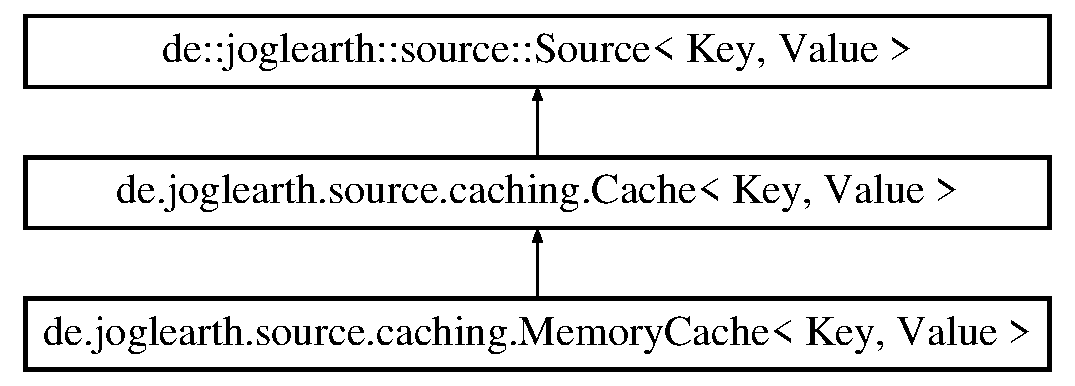
\includegraphics[height=2.000000cm]{interfacede_1_1joglearth_1_1source_1_1caching_1_1_cache_3_01_key_00_01_value_01_4}
\end{center}
\end{figure}
\subsection*{Öffentliche Methoden}
\begin{DoxyCompactItemize}
\item 
void {\bf put\-Object} (Key k, Value v)
\item 
void {\bf drop\-Object} (Key k)
\item 
Iterable$<$ Key $>$ {\bf get\-Existing\-Objects} ()
\item 
void {\bf drop\-All} ()
\end{DoxyCompactItemize}


\subsection{Ausführliche Beschreibung}
Stores objects of type {\ttfamily Value} with an identifier {\ttfamily Key} and returns them on request according to their I\-D. 

\subsection{Dokumentation der Elementfunktionen}
\index{de\-::joglearth\-::source\-::caching\-::\-Cache$<$ Key, Value $>$@{de\-::joglearth\-::source\-::caching\-::\-Cache$<$ Key, Value $>$}!drop\-All@{drop\-All}}
\index{drop\-All@{drop\-All}!de::joglearth::source::caching::Cache< Key, Value >@{de\-::joglearth\-::source\-::caching\-::\-Cache$<$ Key, Value $>$}}
\subsubsection[{drop\-All}]{\setlength{\rightskip}{0pt plus 5cm}void de.\-joglearth.\-source.\-caching.\-Cache$<$ Key, Value $>$.drop\-All (
\begin{DoxyParamCaption}
{}
\end{DoxyParamCaption}
)}\label{interfacede_1_1joglearth_1_1source_1_1caching_1_1_cache_3_01_key_00_01_value_01_4_a5f80139900d2147330955a4bfd865581}
Drops all objects contained in a cache. 

Implementiert in {\bf de.\-joglearth.\-source.\-caching.\-Memory\-Cache$<$ Key, Value $>$} \doxyref{}{S.}{classde_1_1joglearth_1_1source_1_1caching_1_1_memory_cache_3_01_key_00_01_value_01_4_a704e4bb8f34123141f5175f4a22386d0}.

\index{de\-::joglearth\-::source\-::caching\-::\-Cache$<$ Key, Value $>$@{de\-::joglearth\-::source\-::caching\-::\-Cache$<$ Key, Value $>$}!drop\-Object@{drop\-Object}}
\index{drop\-Object@{drop\-Object}!de::joglearth::source::caching::Cache< Key, Value >@{de\-::joglearth\-::source\-::caching\-::\-Cache$<$ Key, Value $>$}}
\subsubsection[{drop\-Object}]{\setlength{\rightskip}{0pt plus 5cm}void de.\-joglearth.\-source.\-caching.\-Cache$<$ Key, Value $>$.drop\-Object (
\begin{DoxyParamCaption}
\item[{Key}]{k}
\end{DoxyParamCaption}
)}\label{interfacede_1_1joglearth_1_1source_1_1caching_1_1_cache_3_01_key_00_01_value_01_4_a8489bd44c6848442a8aa8cc7c4a13cb0}
Erases the reference to an object if the {\ttfamily Key} is a valid I\-D of a stored object.


\begin{DoxyParams}{Parameter}
{\em k} & The I\-D of the object to be dropped \\
\hline
\end{DoxyParams}


Implementiert in {\bf de.\-joglearth.\-source.\-caching.\-Memory\-Cache$<$ Key, Value $>$} \doxyref{}{S.}{classde_1_1joglearth_1_1source_1_1caching_1_1_memory_cache_3_01_key_00_01_value_01_4_a33c591b306da4105b8703321c5765618}.

\index{de\-::joglearth\-::source\-::caching\-::\-Cache$<$ Key, Value $>$@{de\-::joglearth\-::source\-::caching\-::\-Cache$<$ Key, Value $>$}!get\-Existing\-Objects@{get\-Existing\-Objects}}
\index{get\-Existing\-Objects@{get\-Existing\-Objects}!de::joglearth::source::caching::Cache< Key, Value >@{de\-::joglearth\-::source\-::caching\-::\-Cache$<$ Key, Value $>$}}
\subsubsection[{get\-Existing\-Objects}]{\setlength{\rightskip}{0pt plus 5cm}Iterable$<$Key$>$ de.\-joglearth.\-source.\-caching.\-Cache$<$ Key, Value $>$.get\-Existing\-Objects (
\begin{DoxyParamCaption}
{}
\end{DoxyParamCaption}
)}\label{interfacede_1_1joglearth_1_1source_1_1caching_1_1_cache_3_01_key_00_01_value_01_4_a482408fd3c7be507f7d51b421889a725}
Can be used to get the objects that already exist when the cache is initialized. \begin{DoxyReturn}{Rückgabe}
All stored objects 
\end{DoxyReturn}


Implementiert in {\bf de.\-joglearth.\-source.\-caching.\-Memory\-Cache$<$ Key, Value $>$} \doxyref{}{S.}{classde_1_1joglearth_1_1source_1_1caching_1_1_memory_cache_3_01_key_00_01_value_01_4_a98e5a449b0ced05c622c782a8aa1f1ec}.

\index{de\-::joglearth\-::source\-::caching\-::\-Cache$<$ Key, Value $>$@{de\-::joglearth\-::source\-::caching\-::\-Cache$<$ Key, Value $>$}!put\-Object@{put\-Object}}
\index{put\-Object@{put\-Object}!de::joglearth::source::caching::Cache< Key, Value >@{de\-::joglearth\-::source\-::caching\-::\-Cache$<$ Key, Value $>$}}
\subsubsection[{put\-Object}]{\setlength{\rightskip}{0pt plus 5cm}void de.\-joglearth.\-source.\-caching.\-Cache$<$ Key, Value $>$.put\-Object (
\begin{DoxyParamCaption}
\item[{Key}]{k, }
\item[{Value}]{v}
\end{DoxyParamCaption}
)}\label{interfacede_1_1joglearth_1_1source_1_1caching_1_1_cache_3_01_key_00_01_value_01_4_ad2c805820ba476907fd53b4dcb255d50}
Stores object identified by a {\ttfamily Key}. An existing object with that {\ttfamily Key} may be overwritten.


\begin{DoxyParams}{Parameter}
{\em k} & I\-D of the object \\
\hline
{\em v} & The object to be stored \\
\hline
\end{DoxyParams}


Implementiert in {\bf de.\-joglearth.\-source.\-caching.\-Memory\-Cache$<$ Key, Value $>$} \doxyref{}{S.}{classde_1_1joglearth_1_1source_1_1caching_1_1_memory_cache_3_01_key_00_01_value_01_4_a1c757dc21fa73d5318867db45002aae2}.


\section{de.\-joglearth.\-geometry.\-Camera Klassenreferenz}
\label{classde_1_1joglearth_1_1geometry_1_1_camera}\index{de.\-joglearth.\-geometry.\-Camera@{de.\-joglearth.\-geometry.\-Camera}}
\subsection*{Klassen}
\begin{DoxyCompactItemize}
\item 
class {\bfseries Surface\-Height\-Listener}
\end{DoxyCompactItemize}
\subsection*{Öffentliche Methoden}
\begin{DoxyCompactItemize}
\item 
{\bf Camera} ()
\item 
void {\bf set\-Geometry} ({\bf Geometry} g)
\item 
void {\bf set\-Position} ({\bf Geo\-Coordinates} coords)
\item 
void {\bf set\-Distance} (double distance)
\item 
void {\bf set\-Perspective} (double fov, double aspect\-Ratio, double near, double far)
\item 
void {\bf reset\-Tilt} ()
\item 
void {\bf set\-Tilt} (double x, double y)
\item 
void {\bf tilt} (double delta\-X, double delta\-Y)
\item 
void {\bf move} (double delta\-Lon, double delta\-Lat)
\item 
boolean {\bf is\-Point\-Visible} ({\bf Geo\-Coordinates} geo)
\item 
{\bf Screen\-Coordinates} {\bf get\-Screen\-Coordinates} ({\bf Geo\-Coordinates} geo)
\item 
{\bf Geo\-Coordinates} {\bf get\-Geo\-Coordinates} ({\bf Screen\-Coordinates} screen)
\item 
{\bf Tile}[$\,$] {\bf get\-Visible\-Tiles} ()
\item 
{\bf Matrix4} {\bf get\-Projection\-Matrix} ()
\item 
void {\bf add\-Camera\-Listener} ({\bf Camera\-Listener} l)
\item 
void {\bf remove\-Camera\-Listener} ({\bf Camera\-Listener} l)
\end{DoxyCompactItemize}


\subsection{Ausführliche Beschreibung}
Administers geometric calculations for the viewport perspective. 

\subsection{Beschreibung der Konstruktoren und Destruktoren}
\index{de\-::joglearth\-::geometry\-::\-Camera@{de\-::joglearth\-::geometry\-::\-Camera}!Camera@{Camera}}
\index{Camera@{Camera}!de::joglearth::geometry::Camera@{de\-::joglearth\-::geometry\-::\-Camera}}
\subsubsection[{Camera}]{\setlength{\rightskip}{0pt plus 5cm}de.\-joglearth.\-geometry.\-Camera.\-Camera (
\begin{DoxyParamCaption}
{}
\end{DoxyParamCaption}
)}\label{classde_1_1joglearth_1_1geometry_1_1_camera_a29f1c52c4bd14ccbea2b4d6c9413924a}
Constructor.

Creates a \doxyref{de.\-joglearth.\-geometry.\-Camera}{S.}{} with F\-O\-V 90°, aspect ratio 1\-:1, z\-Near=0.\-1 and z\-Far=1000. 

\subsection{Dokumentation der Elementfunktionen}
\index{de\-::joglearth\-::geometry\-::\-Camera@{de\-::joglearth\-::geometry\-::\-Camera}!add\-Camera\-Listener@{add\-Camera\-Listener}}
\index{add\-Camera\-Listener@{add\-Camera\-Listener}!de::joglearth::geometry::Camera@{de\-::joglearth\-::geometry\-::\-Camera}}
\subsubsection[{add\-Camera\-Listener}]{\setlength{\rightskip}{0pt plus 5cm}void de.\-joglearth.\-geometry.\-Camera.\-add\-Camera\-Listener (
\begin{DoxyParamCaption}
\item[{{\bf Camera\-Listener}}]{l}
\end{DoxyParamCaption}
)}\label{classde_1_1joglearth_1_1geometry_1_1_camera_a2f06e1d4b555f4d96f1016e5611568ea}
Adds a new \doxyref{de.\-joglearth.\-geometry.\-Camera\-Listener}{S.}{interfacede_1_1joglearth_1_1geometry_1_1_camera_listener}.


\begin{DoxyParams}{Parameter}
{\em l} & The new {\ttfamily \doxyref{Camera\-Listener}{S.}{interfacede_1_1joglearth_1_1geometry_1_1_camera_listener}} \\
\hline
\end{DoxyParams}
\index{de\-::joglearth\-::geometry\-::\-Camera@{de\-::joglearth\-::geometry\-::\-Camera}!get\-Geo\-Coordinates@{get\-Geo\-Coordinates}}
\index{get\-Geo\-Coordinates@{get\-Geo\-Coordinates}!de::joglearth::geometry::Camera@{de\-::joglearth\-::geometry\-::\-Camera}}
\subsubsection[{get\-Geo\-Coordinates}]{\setlength{\rightskip}{0pt plus 5cm}{\bf Geo\-Coordinates} de.\-joglearth.\-geometry.\-Camera.\-get\-Geo\-Coordinates (
\begin{DoxyParamCaption}
\item[{{\bf Screen\-Coordinates}}]{screen}
\end{DoxyParamCaption}
)}\label{classde_1_1joglearth_1_1geometry_1_1_camera_afe9082eba345c6836dcee5d87ac3d046}
Calculates the longitude and latitude coordinates of the point underneath a point on the screen.


\begin{DoxyParams}{Parameter}
{\em screen} & The screen coordinates \\
\hline
\end{DoxyParams}
\begin{DoxyReturn}{Rückgabe}
The surface coordinates if the point maps to the surface, {\ttfamily null} if it points outside the plane or globe (\char`\"{}space\char`\"{}) 
\end{DoxyReturn}
\index{de\-::joglearth\-::geometry\-::\-Camera@{de\-::joglearth\-::geometry\-::\-Camera}!get\-Projection\-Matrix@{get\-Projection\-Matrix}}
\index{get\-Projection\-Matrix@{get\-Projection\-Matrix}!de::joglearth::geometry::Camera@{de\-::joglearth\-::geometry\-::\-Camera}}
\subsubsection[{get\-Projection\-Matrix}]{\setlength{\rightskip}{0pt plus 5cm}{\bf Matrix4} de.\-joglearth.\-geometry.\-Camera.\-get\-Projection\-Matrix (
\begin{DoxyParamCaption}
{}
\end{DoxyParamCaption}
)}\label{classde_1_1joglearth_1_1geometry_1_1_camera_acddc48206fc1c2374010be00f23e0ef7}
Returns the projection matrix derived from the current camera settings.

The result may be directly passed to Open\-G\-L as a projection matrix, and is guaranteed to produce a picture corresponding to whatever results the camera visibility and projection methods produced for these settings.

\begin{DoxyReturn}{Rückgabe}
The projection matrix 
\end{DoxyReturn}
\index{de\-::joglearth\-::geometry\-::\-Camera@{de\-::joglearth\-::geometry\-::\-Camera}!get\-Screen\-Coordinates@{get\-Screen\-Coordinates}}
\index{get\-Screen\-Coordinates@{get\-Screen\-Coordinates}!de::joglearth::geometry::Camera@{de\-::joglearth\-::geometry\-::\-Camera}}
\subsubsection[{get\-Screen\-Coordinates}]{\setlength{\rightskip}{0pt plus 5cm}{\bf Screen\-Coordinates} de.\-joglearth.\-geometry.\-Camera.\-get\-Screen\-Coordinates (
\begin{DoxyParamCaption}
\item[{{\bf Geo\-Coordinates}}]{geo}
\end{DoxyParamCaption}
)}\label{classde_1_1joglearth_1_1geometry_1_1_camera_a5dcfda10174ad76c0b414afe6478029c}
Calculates the screen coordinates of a visible point given in longitude and latitude coordinates. If the point is not visible, the result is unspecified.


\begin{DoxyParams}{Parameter}
{\em geo} & The point's coordinates \\
\hline
\end{DoxyParams}
\begin{DoxyReturn}{Rückgabe}
The coordinates of the point on the screen 
\end{DoxyReturn}
\index{de\-::joglearth\-::geometry\-::\-Camera@{de\-::joglearth\-::geometry\-::\-Camera}!get\-Visible\-Tiles@{get\-Visible\-Tiles}}
\index{get\-Visible\-Tiles@{get\-Visible\-Tiles}!de::joglearth::geometry::Camera@{de\-::joglearth\-::geometry\-::\-Camera}}
\subsubsection[{get\-Visible\-Tiles}]{\setlength{\rightskip}{0pt plus 5cm}{\bf Tile} [$\,$] de.\-joglearth.\-geometry.\-Camera.\-get\-Visible\-Tiles (
\begin{DoxyParamCaption}
{}
\end{DoxyParamCaption}
)}\label{classde_1_1joglearth_1_1geometry_1_1_camera_aa4704ce2be569a3551d3f43cf5a44646}
Returns an array of tiles visible or partially visible by the \doxyref{de.\-joglearth.\-geometry.\-Camera}{S.}{}.

All tiles have the same detail level, which is calculated from the distance and number of visible tiles.

\begin{DoxyReturn}{Rückgabe}
The array of visible tiles 
\end{DoxyReturn}
\index{de\-::joglearth\-::geometry\-::\-Camera@{de\-::joglearth\-::geometry\-::\-Camera}!is\-Point\-Visible@{is\-Point\-Visible}}
\index{is\-Point\-Visible@{is\-Point\-Visible}!de::joglearth::geometry::Camera@{de\-::joglearth\-::geometry\-::\-Camera}}
\subsubsection[{is\-Point\-Visible}]{\setlength{\rightskip}{0pt plus 5cm}boolean de.\-joglearth.\-geometry.\-Camera.\-is\-Point\-Visible (
\begin{DoxyParamCaption}
\item[{{\bf Geo\-Coordinates}}]{geo}
\end{DoxyParamCaption}
)}\label{classde_1_1joglearth_1_1geometry_1_1_camera_abe19e71f42da5fe01d3515b3efdf5153}
Determines whether a surface point is visible by the \doxyref{de.\-joglearth.\-geometry.\-Camera}{S.}{}. The visibility is limited by both the viewport (the clipping planes) and parts of the scene closer to the camera that might shadow others (the back of the globe, for example).


\begin{DoxyParams}{Parameter}
{\em geo} & The coordinates to check for \\
\hline
\end{DoxyParams}
\begin{DoxyReturn}{Rückgabe}
Whether the point is visible 
\end{DoxyReturn}
\index{de\-::joglearth\-::geometry\-::\-Camera@{de\-::joglearth\-::geometry\-::\-Camera}!move@{move}}
\index{move@{move}!de::joglearth::geometry::Camera@{de\-::joglearth\-::geometry\-::\-Camera}}
\subsubsection[{move}]{\setlength{\rightskip}{0pt plus 5cm}void de.\-joglearth.\-geometry.\-Camera.\-move (
\begin{DoxyParamCaption}
\item[{double}]{delta\-Lon, }
\item[{double}]{delta\-Lat}
\end{DoxyParamCaption}
)}\label{classde_1_1joglearth_1_1geometry_1_1_camera_a69f1e07991f1f7e95e9b3d336a28eeb6}
Changes the surface position of the \doxyref{de.\-joglearth.\-geometry.\-Camera}{S.}{} by difference values.


\begin{DoxyParams}{Parameter}
{\em delta\-Lon} & The angular distance to move in longitude direction \\
\hline
{\em delta\-Lat} & The angular distance to move in latitude direction \\
\hline
\end{DoxyParams}
\index{de\-::joglearth\-::geometry\-::\-Camera@{de\-::joglearth\-::geometry\-::\-Camera}!remove\-Camera\-Listener@{remove\-Camera\-Listener}}
\index{remove\-Camera\-Listener@{remove\-Camera\-Listener}!de::joglearth::geometry::Camera@{de\-::joglearth\-::geometry\-::\-Camera}}
\subsubsection[{remove\-Camera\-Listener}]{\setlength{\rightskip}{0pt plus 5cm}void de.\-joglearth.\-geometry.\-Camera.\-remove\-Camera\-Listener (
\begin{DoxyParamCaption}
\item[{{\bf Camera\-Listener}}]{l}
\end{DoxyParamCaption}
)}\label{classde_1_1joglearth_1_1geometry_1_1_camera_a961ca081f11f43f651e6691c953efb79}
Removes a given \doxyref{de.\-joglearth.\-geometry.\-Camera\-Listener}{S.}{interfacede_1_1joglearth_1_1geometry_1_1_camera_listener}.


\begin{DoxyParams}{Parameter}
{\em l} & The {\ttfamily \doxyref{Camera\-Listener}{S.}{interfacede_1_1joglearth_1_1geometry_1_1_camera_listener}} that should be removed \\
\hline
\end{DoxyParams}
\index{de\-::joglearth\-::geometry\-::\-Camera@{de\-::joglearth\-::geometry\-::\-Camera}!reset\-Tilt@{reset\-Tilt}}
\index{reset\-Tilt@{reset\-Tilt}!de::joglearth::geometry::Camera@{de\-::joglearth\-::geometry\-::\-Camera}}
\subsubsection[{reset\-Tilt}]{\setlength{\rightskip}{0pt plus 5cm}void de.\-joglearth.\-geometry.\-Camera.\-reset\-Tilt (
\begin{DoxyParamCaption}
{}
\end{DoxyParamCaption}
)}\label{classde_1_1joglearth_1_1geometry_1_1_camera_ab06fa6de4a7d086eea9d11ed94936b8c}
Resets the \doxyref{de.\-joglearth.\-geometry.\-Camera}{S.}{} tilt to x=y=0. \index{de\-::joglearth\-::geometry\-::\-Camera@{de\-::joglearth\-::geometry\-::\-Camera}!set\-Distance@{set\-Distance}}
\index{set\-Distance@{set\-Distance}!de::joglearth::geometry::Camera@{de\-::joglearth\-::geometry\-::\-Camera}}
\subsubsection[{set\-Distance}]{\setlength{\rightskip}{0pt plus 5cm}void de.\-joglearth.\-geometry.\-Camera.\-set\-Distance (
\begin{DoxyParamCaption}
\item[{double}]{distance}
\end{DoxyParamCaption}
)}\label{classde_1_1joglearth_1_1geometry_1_1_camera_a6aeda520b06ed43cd8cd322cad50b5e5}
Sets the \doxyref{de.\-joglearth.\-geometry.\-Camera}{S.}{}'s distance to the surface.


\begin{DoxyParams}{Parameter}
{\em distance} & The distance \\
\hline
\end{DoxyParams}
\index{de\-::joglearth\-::geometry\-::\-Camera@{de\-::joglearth\-::geometry\-::\-Camera}!set\-Geometry@{set\-Geometry}}
\index{set\-Geometry@{set\-Geometry}!de::joglearth::geometry::Camera@{de\-::joglearth\-::geometry\-::\-Camera}}
\subsubsection[{set\-Geometry}]{\setlength{\rightskip}{0pt plus 5cm}void de.\-joglearth.\-geometry.\-Camera.\-set\-Geometry (
\begin{DoxyParamCaption}
\item[{{\bf Geometry}}]{g}
\end{DoxyParamCaption}
)}\label{classde_1_1joglearth_1_1geometry_1_1_camera_a7a517b53cbcfabacfeaed8fd6c8b5b63}
Sets a new \doxyref{de.\-joglearth.\-geometry.\-Geometry}{S.}{interfacede_1_1joglearth_1_1geometry_1_1_geometry} object for model-\/specific computations.


\begin{DoxyParams}{Parameter}
{\em g} & The new \doxyref{Geometry}{S.}{interfacede_1_1joglearth_1_1geometry_1_1_geometry} object \\
\hline
\end{DoxyParams}
\index{de\-::joglearth\-::geometry\-::\-Camera@{de\-::joglearth\-::geometry\-::\-Camera}!set\-Perspective@{set\-Perspective}}
\index{set\-Perspective@{set\-Perspective}!de::joglearth::geometry::Camera@{de\-::joglearth\-::geometry\-::\-Camera}}
\subsubsection[{set\-Perspective}]{\setlength{\rightskip}{0pt plus 5cm}void de.\-joglearth.\-geometry.\-Camera.\-set\-Perspective (
\begin{DoxyParamCaption}
\item[{double}]{fov, }
\item[{double}]{aspect\-Ratio, }
\item[{double}]{near, }
\item[{double}]{far}
\end{DoxyParamCaption}
)}\label{classde_1_1joglearth_1_1geometry_1_1_camera_adb41b643cb5880cb93b32744ffaee1a1}
Sets the parameters for the perspective transformation done by the projection matrix.


\begin{DoxyParams}{Parameter}
{\em fov} & The field of view, in radians. This is the angular distance of the left and right clipping plane. 90° (P\-I/2) by default \\
\hline
{\em aspect\-Ratio} & The aspect ratio, i.\-e. the width-\/to-\/height ratio. 1 by default \\
\hline
{\em near} & The distance of the near clipping plane to the camera position. 0.\-1 by default \\
\hline
{\em far} & The distance of the far clipping plane to the camera position. 1000.\-0 by default \\
\hline
\end{DoxyParams}
\index{de\-::joglearth\-::geometry\-::\-Camera@{de\-::joglearth\-::geometry\-::\-Camera}!set\-Position@{set\-Position}}
\index{set\-Position@{set\-Position}!de::joglearth::geometry::Camera@{de\-::joglearth\-::geometry\-::\-Camera}}
\subsubsection[{set\-Position}]{\setlength{\rightskip}{0pt plus 5cm}void de.\-joglearth.\-geometry.\-Camera.\-set\-Position (
\begin{DoxyParamCaption}
\item[{{\bf Geo\-Coordinates}}]{coords}
\end{DoxyParamCaption}
)}\label{classde_1_1joglearth_1_1geometry_1_1_camera_accb57080d3b54b039dd2c319888456d0}
Sets the position the \doxyref{de.\-joglearth.\-geometry.\-Camera}{S.}{} is currently over.


\begin{DoxyParams}{Parameter}
{\em coords} & The {\ttfamily \doxyref{Geo\-Coordinates}{S.}{classde_1_1joglearth_1_1geometry_1_1_geo_coordinates}} of the camera's position \\
\hline
\end{DoxyParams}
\index{de\-::joglearth\-::geometry\-::\-Camera@{de\-::joglearth\-::geometry\-::\-Camera}!set\-Tilt@{set\-Tilt}}
\index{set\-Tilt@{set\-Tilt}!de::joglearth::geometry::Camera@{de\-::joglearth\-::geometry\-::\-Camera}}
\subsubsection[{set\-Tilt}]{\setlength{\rightskip}{0pt plus 5cm}void de.\-joglearth.\-geometry.\-Camera.\-set\-Tilt (
\begin{DoxyParamCaption}
\item[{double}]{x, }
\item[{double}]{y}
\end{DoxyParamCaption}
)}\label{classde_1_1joglearth_1_1geometry_1_1_camera_aae972a16bed0d01cebb14fd006ab16eb}
Sets the \doxyref{de.\-joglearth.\-geometry.\-Camera}{S.}{} tilt to a specific value.


\begin{DoxyParams}{Parameter}
{\em x} & The tilt around the x axis (\char`\"{}up and down\char`\"{}) \\
\hline
{\em y} & The tilt around the y axis (\char`\"{}left and right\char`\"{}) \\
\hline
\end{DoxyParams}
\index{de\-::joglearth\-::geometry\-::\-Camera@{de\-::joglearth\-::geometry\-::\-Camera}!tilt@{tilt}}
\index{tilt@{tilt}!de::joglearth::geometry::Camera@{de\-::joglearth\-::geometry\-::\-Camera}}
\subsubsection[{tilt}]{\setlength{\rightskip}{0pt plus 5cm}void de.\-joglearth.\-geometry.\-Camera.\-tilt (
\begin{DoxyParamCaption}
\item[{double}]{delta\-X, }
\item[{double}]{delta\-Y}
\end{DoxyParamCaption}
)}\label{classde_1_1joglearth_1_1geometry_1_1_camera_ad33f6da0b82dd367ecbd99dc98c3d4db}
Changes the tilt by a difference value.


\begin{DoxyParams}{Parameter}
{\em delta\-X} & The tilt difference around the x axis (\char`\"{}up and down\char`\"{}) \\
\hline
{\em delta\-Y} & The tilt difference around the y axis (\char`\"{}left and right\char`\"{}) \\
\hline
\end{DoxyParams}

\section{de.\-joglearth.\-geometry.\-Camera\-Listener Schnittstellenreferenz}
\label{interfacede_1_1joglearth_1_1geometry_1_1_camera_listener}\index{de.\-joglearth.\-geometry.\-Camera\-Listener@{de.\-joglearth.\-geometry.\-Camera\-Listener}}


Basisklasse für de.\-joglearth.\-ui.\-Main\-Window.\-U\-I\-Camera\-Listener.

\subsection*{Öffentliche Methoden}
\begin{DoxyCompactItemize}
\item 
void {\bf camera\-View\-Changed} ()
\end{DoxyCompactItemize}


\subsection{Ausführliche Beschreibung}
Listener interface notified when the view parameters of a \doxyref{de.\-joglearth.\-geometry.\-Camera}{S.}{classde_1_1joglearth_1_1geometry_1_1_camera} are changed. 

\subsection{Dokumentation der Elementfunktionen}
\index{de\-::joglearth\-::geometry\-::\-Camera\-Listener@{de\-::joglearth\-::geometry\-::\-Camera\-Listener}!camera\-View\-Changed@{camera\-View\-Changed}}
\index{camera\-View\-Changed@{camera\-View\-Changed}!de::joglearth::geometry::CameraListener@{de\-::joglearth\-::geometry\-::\-Camera\-Listener}}
\subsubsection[{camera\-View\-Changed}]{\setlength{\rightskip}{0pt plus 5cm}void de.\-joglearth.\-geometry.\-Camera\-Listener.\-camera\-View\-Changed (
\begin{DoxyParamCaption}
{}
\end{DoxyParamCaption}
)}\label{interfacede_1_1joglearth_1_1geometry_1_1_camera_listener_a960186d2b50619ee65dddcf5058ba608}
Is called whenever a setting of the \doxyref{de.\-joglearth.\-geometry.\-Camera}{S.}{classde_1_1joglearth_1_1geometry_1_1_camera} changes. 
\section{de.\-joglearth.\-rendering.\-Display\-Mode Enum-\/\-Referenz}
\label{enumde_1_1joglearth_1_1rendering_1_1_display_mode}\index{de.\-joglearth.\-rendering.\-Display\-Mode@{de.\-joglearth.\-rendering.\-Display\-Mode}}
\subsection*{Öffentliche Attribute}
\begin{DoxyCompactItemize}
\item 
{\bf S\-O\-L\-A\-R\-\_\-\-S\-Y\-S\-T\-E\-M}
\item 
{\bf G\-L\-O\-B\-E\-\_\-\-M\-A\-P}
\item 
{\bf P\-L\-A\-N\-E\-\_\-\-M\-A\-P}
\end{DoxyCompactItemize}


\subsection{Ausführliche Beschreibung}
Enumerates the display modes supported by the \doxyref{Renderer}{S.}{classde_1_1joglearth_1_1rendering_1_1_renderer}. 

\subsection{Dokumentation der Datenelemente}
\index{de\-::joglearth\-::rendering\-::\-Display\-Mode@{de\-::joglearth\-::rendering\-::\-Display\-Mode}!G\-L\-O\-B\-E\-\_\-\-M\-A\-P@{G\-L\-O\-B\-E\-\_\-\-M\-A\-P}}
\index{G\-L\-O\-B\-E\-\_\-\-M\-A\-P@{G\-L\-O\-B\-E\-\_\-\-M\-A\-P}!de::joglearth::rendering::DisplayMode@{de\-::joglearth\-::rendering\-::\-Display\-Mode}}
\subsubsection[{G\-L\-O\-B\-E\-\_\-\-M\-A\-P}]{\setlength{\rightskip}{0pt plus 5cm}de.\-joglearth.\-rendering.\-Display\-Mode.\-G\-L\-O\-B\-E\-\_\-\-M\-A\-P}\label{enumde_1_1joglearth_1_1rendering_1_1_display_mode_a90eb7b0d25f2366c39eb5c656fd1be43}
Shows maps on the globe's surface. \index{de\-::joglearth\-::rendering\-::\-Display\-Mode@{de\-::joglearth\-::rendering\-::\-Display\-Mode}!P\-L\-A\-N\-E\-\_\-\-M\-A\-P@{P\-L\-A\-N\-E\-\_\-\-M\-A\-P}}
\index{P\-L\-A\-N\-E\-\_\-\-M\-A\-P@{P\-L\-A\-N\-E\-\_\-\-M\-A\-P}!de::joglearth::rendering::DisplayMode@{de\-::joglearth\-::rendering\-::\-Display\-Mode}}
\subsubsection[{P\-L\-A\-N\-E\-\_\-\-M\-A\-P}]{\setlength{\rightskip}{0pt plus 5cm}de.\-joglearth.\-rendering.\-Display\-Mode.\-P\-L\-A\-N\-E\-\_\-\-M\-A\-P}\label{enumde_1_1joglearth_1_1rendering_1_1_display_mode_a9c02f1e286c8f73bae05b3c18c3b4773}
Shows maps on a plane surface. \index{de\-::joglearth\-::rendering\-::\-Display\-Mode@{de\-::joglearth\-::rendering\-::\-Display\-Mode}!S\-O\-L\-A\-R\-\_\-\-S\-Y\-S\-T\-E\-M@{S\-O\-L\-A\-R\-\_\-\-S\-Y\-S\-T\-E\-M}}
\index{S\-O\-L\-A\-R\-\_\-\-S\-Y\-S\-T\-E\-M@{S\-O\-L\-A\-R\-\_\-\-S\-Y\-S\-T\-E\-M}!de::joglearth::rendering::DisplayMode@{de\-::joglearth\-::rendering\-::\-Display\-Mode}}
\subsubsection[{S\-O\-L\-A\-R\-\_\-\-S\-Y\-S\-T\-E\-M}]{\setlength{\rightskip}{0pt plus 5cm}de.\-joglearth.\-rendering.\-Display\-Mode.\-S\-O\-L\-A\-R\-\_\-\-S\-Y\-S\-T\-E\-M}\label{enumde_1_1joglearth_1_1rendering_1_1_display_mode_a1de006693f755572b8b40ab9166da082}
Shows a solar system demo. 
\section{de.\-joglearth.\-source.\-caching.\-File\-System\-Cache$<$ Key $>$ Klassenreferenz}
\label{classde_1_1joglearth_1_1source_1_1caching_1_1_file_system_cache_3_01_key_01_4}\index{de.\-joglearth.\-source.\-caching.\-File\-System\-Cache$<$ Key $>$@{de.\-joglearth.\-source.\-caching.\-File\-System\-Cache$<$ Key $>$}}


Abgeleitet von Cache$<$ Key, byte[$\,$]$>$.

\subsection*{Öffentliche Methoden}
\begin{DoxyCompactItemize}
\item 
{\bf File\-System\-Cache} (String folder, Path\-Translator$<$ Key $>$ p)
\item 
Source\-Response$<$ byte[$\,$]$>$ {\bfseries request\-Object} (Key key, Source\-Listener$<$ Key, byte[$\,$]$>$ sender)\label{classde_1_1joglearth_1_1source_1_1caching_1_1_file_system_cache_3_01_key_01_4_ae40d9dd9583027c14e4468e183cf48da}

\item 
void {\bfseries put\-Object} (Key k, byte[$\,$] v)\label{classde_1_1joglearth_1_1source_1_1caching_1_1_file_system_cache_3_01_key_01_4_a0dcec50e30bb7f6356c7bf56ed386428}

\item 
void {\bfseries drop\-Object} (Key k)\label{classde_1_1joglearth_1_1source_1_1caching_1_1_file_system_cache_3_01_key_01_4_ae118a62fab9e478561d9a5ec7077901d}

\item 
Iterable$<$ Key $>$ {\bfseries get\-Existing\-Objects} ()\label{classde_1_1joglearth_1_1source_1_1caching_1_1_file_system_cache_3_01_key_01_4_a3b91ae313313eb6306e7af7997ab3dda}

\item 
void {\bfseries drop\-All} ()\label{classde_1_1joglearth_1_1source_1_1caching_1_1_file_system_cache_3_01_key_01_4_a433d8c26ced086c0cda87ebd1a072765}

\end{DoxyCompactItemize}


\subsection{Ausführliche Beschreibung}
Implements the \doxyref{de.\-jogl\-Earth.\-source.\-caching.\-Cache}{S.}{} interface in such way that it stores objects in the file system. 

\subsection{Beschreibung der Konstruktoren und Destruktoren}
\index{de\-::joglearth\-::source\-::caching\-::\-File\-System\-Cache$<$ Key $>$@{de\-::joglearth\-::source\-::caching\-::\-File\-System\-Cache$<$ Key $>$}!File\-System\-Cache@{File\-System\-Cache}}
\index{File\-System\-Cache@{File\-System\-Cache}!de::joglearth::source::caching::FileSystemCache< Key >@{de\-::joglearth\-::source\-::caching\-::\-File\-System\-Cache$<$ Key $>$}}
\subsubsection[{File\-System\-Cache}]{\setlength{\rightskip}{0pt plus 5cm}de.\-joglearth.\-source.\-caching.\-File\-System\-Cache$<$ Key $>$.File\-System\-Cache (
\begin{DoxyParamCaption}
\item[{String}]{folder, }
\item[{Path\-Translator$<$ Key $>$}]{p}
\end{DoxyParamCaption}
)}\label{classde_1_1joglearth_1_1source_1_1caching_1_1_file_system_cache_3_01_key_01_4_aa15baef0f6d76f03f3b24a2b26217251}
Constructor.\-Initializes a {\ttfamily File\-System\-Cache} as it assigns values to the {\ttfamily folder} value and the \doxyref{de.\-jogl\-Earth.\-source.\-caching.\-Path\-Translator}{S.}{}.


\begin{DoxyParams}{Parameter}
{\em folder} & The name of the folder where the objects should be stored \\
\hline
{\em p} & The {\ttfamily Path\-Translator} that is used by the {\ttfamily File\-System\-Cache} to convert a path to a string and vice versa \\
\hline
\end{DoxyParams}

\section{de.\-joglearth.\-geometry.\-Geo\-Coordinates Klassenreferenz}
\label{classde_1_1joglearth_1_1geometry_1_1_geo_coordinates}\index{de.\-joglearth.\-geometry.\-Geo\-Coordinates@{de.\-joglearth.\-geometry.\-Geo\-Coordinates}}
\subsection*{Öffentliche Methoden}
\begin{DoxyCompactItemize}
\item 
{\bf Geo\-Coordinates} (double lon, double lat)
\item 
{\bf Geo\-Coordinates} {\bfseries clone} ()\label{classde_1_1joglearth_1_1geometry_1_1_geo_coordinates_a22d4ebdf5eb872c5a9f20bf204cf036c}

\item 
double {\bf get\-Longitude} ()
\item 
double {\bf get\-Latitude} ()
\item 
String {\bf get\-Longitude\-String} ()
\item 
String {\bf get\-Latitude\-String} ()
\item 
String {\bfseries to\-String} ()\label{classde_1_1joglearth_1_1geometry_1_1_geo_coordinates_aeff694f70cbb07e5185ec3caa30ec632}

\item 
int {\bfseries hash\-Code} ()\label{classde_1_1joglearth_1_1geometry_1_1_geo_coordinates_a788cc2e0c94e6c7d1b614a63b30c1c98}

\item 
boolean {\bfseries equals} (Object obj)\label{classde_1_1joglearth_1_1geometry_1_1_geo_coordinates_ac5c4def2c19cd4a32dc90a77158ba9c1}

\end{DoxyCompactItemize}
\subsection*{Öffentliche, statische Methoden}
\begin{DoxyCompactItemize}
\item 
static double {\bfseries rad\-To\-Deg} (double rad)\label{classde_1_1joglearth_1_1geometry_1_1_geo_coordinates_ab337427f199f610f13d503b71e9731f1}

\item 
static double {\bfseries limit\-Rad} (double rad)\label{classde_1_1joglearth_1_1geometry_1_1_geo_coordinates_ac2bf9ff7e17192132ec0af9add1d7cb6}

\item 
static {\bf Geo\-Coordinates} {\bf parse\-Coordinates} (String lon, String lat)
\end{DoxyCompactItemize}


\subsection{Ausführliche Beschreibung}
Structure holding longitude and latitude coordinates. 

\subsection{Beschreibung der Konstruktoren und Destruktoren}
\index{de\-::joglearth\-::geometry\-::\-Geo\-Coordinates@{de\-::joglearth\-::geometry\-::\-Geo\-Coordinates}!Geo\-Coordinates@{Geo\-Coordinates}}
\index{Geo\-Coordinates@{Geo\-Coordinates}!de::joglearth::geometry::GeoCoordinates@{de\-::joglearth\-::geometry\-::\-Geo\-Coordinates}}
\subsubsection[{Geo\-Coordinates}]{\setlength{\rightskip}{0pt plus 5cm}de.\-joglearth.\-geometry.\-Geo\-Coordinates.\-Geo\-Coordinates (
\begin{DoxyParamCaption}
\item[{double}]{lon, }
\item[{double}]{lat}
\end{DoxyParamCaption}
)}\label{classde_1_1joglearth_1_1geometry_1_1_geo_coordinates_ab85b161624d8f1715b7ceb2d1fff1627}
Constructor. Initializes coordinates by their values in radians.


\begin{DoxyParams}{Parameter}
{\em lon} & Longitude, in the interval [0, 2pi) \\
\hline
{\em lat} & Latitude, in the interval [-\/pi/2, pi/2] \\
\hline
\end{DoxyParams}


\subsection{Dokumentation der Elementfunktionen}
\index{de\-::joglearth\-::geometry\-::\-Geo\-Coordinates@{de\-::joglearth\-::geometry\-::\-Geo\-Coordinates}!get\-Latitude@{get\-Latitude}}
\index{get\-Latitude@{get\-Latitude}!de::joglearth::geometry::GeoCoordinates@{de\-::joglearth\-::geometry\-::\-Geo\-Coordinates}}
\subsubsection[{get\-Latitude}]{\setlength{\rightskip}{0pt plus 5cm}double de.\-joglearth.\-geometry.\-Geo\-Coordinates.\-get\-Latitude (
\begin{DoxyParamCaption}
{}
\end{DoxyParamCaption}
)}\label{classde_1_1joglearth_1_1geometry_1_1_geo_coordinates_aab194fa19c1cd0278a0a46593d02f491}
Returns the latitude, in radians. \begin{DoxyReturn}{Rückgabe}
The latitude 
\end{DoxyReturn}
\index{de\-::joglearth\-::geometry\-::\-Geo\-Coordinates@{de\-::joglearth\-::geometry\-::\-Geo\-Coordinates}!get\-Latitude\-String@{get\-Latitude\-String}}
\index{get\-Latitude\-String@{get\-Latitude\-String}!de::joglearth::geometry::GeoCoordinates@{de\-::joglearth\-::geometry\-::\-Geo\-Coordinates}}
\subsubsection[{get\-Latitude\-String}]{\setlength{\rightskip}{0pt plus 5cm}String de.\-joglearth.\-geometry.\-Geo\-Coordinates.\-get\-Latitude\-String (
\begin{DoxyParamCaption}
{}
\end{DoxyParamCaption}
)}\label{classde_1_1joglearth_1_1geometry_1_1_geo_coordinates_acc254db595ec834590276598ba933962}
Returns a string describing the latitude. \begin{DoxyReturn}{Rückgabe}
The latitude in string representation 
\end{DoxyReturn}
\index{de\-::joglearth\-::geometry\-::\-Geo\-Coordinates@{de\-::joglearth\-::geometry\-::\-Geo\-Coordinates}!get\-Longitude@{get\-Longitude}}
\index{get\-Longitude@{get\-Longitude}!de::joglearth::geometry::GeoCoordinates@{de\-::joglearth\-::geometry\-::\-Geo\-Coordinates}}
\subsubsection[{get\-Longitude}]{\setlength{\rightskip}{0pt plus 5cm}double de.\-joglearth.\-geometry.\-Geo\-Coordinates.\-get\-Longitude (
\begin{DoxyParamCaption}
{}
\end{DoxyParamCaption}
)}\label{classde_1_1joglearth_1_1geometry_1_1_geo_coordinates_a0131884b84fd9c888ebfea83d106213b}
Returns the longitude, in radians. \begin{DoxyReturn}{Rückgabe}
The longitude 
\end{DoxyReturn}
\index{de\-::joglearth\-::geometry\-::\-Geo\-Coordinates@{de\-::joglearth\-::geometry\-::\-Geo\-Coordinates}!get\-Longitude\-String@{get\-Longitude\-String}}
\index{get\-Longitude\-String@{get\-Longitude\-String}!de::joglearth::geometry::GeoCoordinates@{de\-::joglearth\-::geometry\-::\-Geo\-Coordinates}}
\subsubsection[{get\-Longitude\-String}]{\setlength{\rightskip}{0pt plus 5cm}String de.\-joglearth.\-geometry.\-Geo\-Coordinates.\-get\-Longitude\-String (
\begin{DoxyParamCaption}
{}
\end{DoxyParamCaption}
)}\label{classde_1_1joglearth_1_1geometry_1_1_geo_coordinates_ae1efcb3ef78bc9c724677c18e479df9f}
Returns a string describing the longitude. \begin{DoxyReturn}{Rückgabe}
The longitude in string representation 
\end{DoxyReturn}
\index{de\-::joglearth\-::geometry\-::\-Geo\-Coordinates@{de\-::joglearth\-::geometry\-::\-Geo\-Coordinates}!parse\-Coordinates@{parse\-Coordinates}}
\index{parse\-Coordinates@{parse\-Coordinates}!de::joglearth::geometry::GeoCoordinates@{de\-::joglearth\-::geometry\-::\-Geo\-Coordinates}}
\subsubsection[{parse\-Coordinates}]{\setlength{\rightskip}{0pt plus 5cm}static {\bf Geo\-Coordinates} de.\-joglearth.\-geometry.\-Geo\-Coordinates.\-parse\-Coordinates (
\begin{DoxyParamCaption}
\item[{String}]{lon, }
\item[{String}]{lat}
\end{DoxyParamCaption}
)\hspace{0.3cm}{\ttfamily [static]}}\label{classde_1_1joglearth_1_1geometry_1_1_geo_coordinates_a51b1d3e2b1645918bf77e9162dab8008}
Parses two coordinate strings, returning the \doxyref{Geo\-Coordinates}{S.}{classde_1_1joglearth_1_1geometry_1_1_geo_coordinates}.


\begin{DoxyParams}{Parameter}
{\em lon} & The longitude, e.\-g. 55° 17' 48.\-2\char`\"{} E
@param lat The latitude, e.\-g. 55° 17' 48.\-2\char`\"{} N \\
\hline
\end{DoxyParams}
\begin{DoxyReturn}{Rückgabe}
The coordinate structure 
\end{DoxyReturn}

\begin{DoxyExceptions}{Ausnahmebehandlung}
{\em Number\-Format\-Exception} & One of the parameters was not a valid coordinate \\
\hline
\end{DoxyExceptions}

\section{de.\-joglearth.\-geometry.\-Geometry Schnittstellenreferenz}
\label{interfacede_1_1joglearth_1_1geometry_1_1_geometry}\index{de.\-joglearth.\-geometry.\-Geometry@{de.\-joglearth.\-geometry.\-Geometry}}
Klassendiagramm für de.\-joglearth.\-geometry.\-Geometry\-:\begin{figure}[H]
\begin{center}
\leavevmode
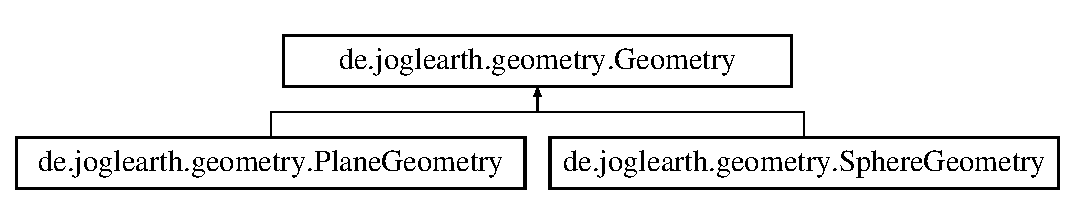
\includegraphics[height=2.000000cm]{interfacede_1_1joglearth_1_1geometry_1_1_geometry}
\end{center}
\end{figure}
\subsection*{Öffentliche Methoden}
\begin{DoxyCompactItemize}
\item 
boolean {\bf is\-Point\-Visible} ({\bf Geo\-Coordinates} geo)
\item 
{\bf Vector3} {\bf get\-Space\-Position} ({\bf Geo\-Coordinates} geo)
\item 
{\bf Screen\-Coordinates} {\bf get\-Surface\-Coordinates} ({\bf Vector3} camera\-Position, {\bf Vector3} view\-Vector)
\item 
{\bf Matrix4} {\bf get\-View\-Matrix} ()
\end{DoxyCompactItemize}


\subsection{Ausführliche Beschreibung}
Abstracts geometric calculations dependent on the map model (plane or sphere). 

\subsection{Dokumentation der Elementfunktionen}
\index{de\-::joglearth\-::geometry\-::\-Geometry@{de\-::joglearth\-::geometry\-::\-Geometry}!get\-Space\-Position@{get\-Space\-Position}}
\index{get\-Space\-Position@{get\-Space\-Position}!de::joglearth::geometry::Geometry@{de\-::joglearth\-::geometry\-::\-Geometry}}
\subsubsection[{get\-Space\-Position}]{\setlength{\rightskip}{0pt plus 5cm}{\bf Vector3} de.\-joglearth.\-geometry.\-Geometry.\-get\-Space\-Position (
\begin{DoxyParamCaption}
\item[{{\bf Geo\-Coordinates}}]{geo}
\end{DoxyParamCaption}
)}\label{interfacede_1_1joglearth_1_1geometry_1_1_geometry_a8fa1da4fcc3f99eb998a5db2f22cb2eb}
Determines the three-\/dimensional position of a surface point in model space. The height map is ignored.


\begin{DoxyParams}{Parameter}
{\em geo} & The surface point \\
\hline
\end{DoxyParams}
\begin{DoxyReturn}{Rückgabe}
The position 
\end{DoxyReturn}


Implementiert in {\bf de.\-joglearth.\-geometry.\-Plane\-Geometry} \doxyref{}{S.}{classde_1_1joglearth_1_1geometry_1_1_plane_geometry_a1ea89c7fd032ef989112538321d0c91d} und {\bf de.\-joglearth.\-geometry.\-Sphere\-Geometry} \doxyref{}{S.}{classde_1_1joglearth_1_1geometry_1_1_sphere_geometry_a058f9d046e2c3d7dd26747eec134d0a1}.

\index{de\-::joglearth\-::geometry\-::\-Geometry@{de\-::joglearth\-::geometry\-::\-Geometry}!get\-Surface\-Coordinates@{get\-Surface\-Coordinates}}
\index{get\-Surface\-Coordinates@{get\-Surface\-Coordinates}!de::joglearth::geometry::Geometry@{de\-::joglearth\-::geometry\-::\-Geometry}}
\subsubsection[{get\-Surface\-Coordinates}]{\setlength{\rightskip}{0pt plus 5cm}{\bf Screen\-Coordinates} de.\-joglearth.\-geometry.\-Geometry.\-get\-Surface\-Coordinates (
\begin{DoxyParamCaption}
\item[{{\bf Vector3}}]{camera\-Position, }
\item[{{\bf Vector3}}]{view\-Vector}
\end{DoxyParamCaption}
)}\label{interfacede_1_1joglearth_1_1geometry_1_1_geometry_a9d4503c3c7e6fab0fd6535864105d155}
Calculates the surface coordinates of the intersection from a straight line between a given point and the model center (The globes center or infinity for the map plane) and the map surface.


\begin{DoxyParams}{Parameter}
{\em view\-Vector} & The origin point \\
\hline
\end{DoxyParams}
\begin{DoxyReturn}{Rückgabe}
The surface coordinates 
\end{DoxyReturn}


Implementiert in {\bf de.\-joglearth.\-geometry.\-Plane\-Geometry} \doxyref{}{S.}{classde_1_1joglearth_1_1geometry_1_1_plane_geometry_a3a410f67e2a77dd0a9010ce00af7781e} und {\bf de.\-joglearth.\-geometry.\-Sphere\-Geometry} \doxyref{}{S.}{classde_1_1joglearth_1_1geometry_1_1_sphere_geometry_a0647b58a7956281dbe3cdd6aa84cc497}.

\index{de\-::joglearth\-::geometry\-::\-Geometry@{de\-::joglearth\-::geometry\-::\-Geometry}!get\-View\-Matrix@{get\-View\-Matrix}}
\index{get\-View\-Matrix@{get\-View\-Matrix}!de::joglearth::geometry::Geometry@{de\-::joglearth\-::geometry\-::\-Geometry}}
\subsubsection[{get\-View\-Matrix}]{\setlength{\rightskip}{0pt plus 5cm}{\bf Matrix4} de.\-joglearth.\-geometry.\-Geometry.\-get\-View\-Matrix (
\begin{DoxyParamCaption}
{}
\end{DoxyParamCaption}
)}\label{interfacede_1_1joglearth_1_1geometry_1_1_geometry_a30f45d30257e8fc7e9d6f91cf846cdda}
Returns the view matrix performing translations and rotations incurred by the camera position.

\begin{DoxyReturn}{Rückgabe}
The view matrix 
\end{DoxyReturn}


Implementiert in {\bf de.\-joglearth.\-geometry.\-Plane\-Geometry} \doxyref{}{S.}{classde_1_1joglearth_1_1geometry_1_1_plane_geometry_a27f961bb318adbeec26f5cb930a35877} und {\bf de.\-joglearth.\-geometry.\-Sphere\-Geometry} \doxyref{}{S.}{classde_1_1joglearth_1_1geometry_1_1_sphere_geometry_adaebcd9cc9c9e5c6146dd699c701cdba}.

\index{de\-::joglearth\-::geometry\-::\-Geometry@{de\-::joglearth\-::geometry\-::\-Geometry}!is\-Point\-Visible@{is\-Point\-Visible}}
\index{is\-Point\-Visible@{is\-Point\-Visible}!de::joglearth::geometry::Geometry@{de\-::joglearth\-::geometry\-::\-Geometry}}
\subsubsection[{is\-Point\-Visible}]{\setlength{\rightskip}{0pt plus 5cm}boolean de.\-joglearth.\-geometry.\-Geometry.\-is\-Point\-Visible (
\begin{DoxyParamCaption}
\item[{{\bf Geo\-Coordinates}}]{geo}
\end{DoxyParamCaption}
)}\label{interfacede_1_1joglearth_1_1geometry_1_1_geometry_a1bca475164a399431f9f6238dd292b6a}
Returns whether a point, given by longitude and latitude coordinates, could be visible provided that the field of view and distance are large enough.


\begin{DoxyParams}{Parameter}
{\em geo} & The surface point \\
\hline
\end{DoxyParams}
\begin{DoxyReturn}{Rückgabe}
Whether the point might be visible 
\end{DoxyReturn}


Implementiert in {\bf de.\-joglearth.\-geometry.\-Plane\-Geometry} \doxyref{}{S.}{classde_1_1joglearth_1_1geometry_1_1_plane_geometry_acd7ef9b8485c8be9056583ab441976e2} und {\bf de.\-joglearth.\-geometry.\-Sphere\-Geometry} \doxyref{}{S.}{classde_1_1joglearth_1_1geometry_1_1_sphere_geometry_a224b024410063b95a3ec51fcc983effb}.


\section{de.\-joglearth.\-surface.\-Height\-Map Klassenreferenz}
\label{classde_1_1joglearth_1_1surface_1_1_height_map}\index{de.\-joglearth.\-surface.\-Height\-Map@{de.\-joglearth.\-surface.\-Height\-Map}}
\subsection*{Öffentliche, statische Methoden}
\begin{DoxyCompactItemize}
\item 
static double {\bf get\-Height} ({\bf Geo\-Coordinates} coords)
\item 
static void {\bf add\-Surface\-Listener} ({\bf Surface\-Listener} l)
\item 
static void {\bf remove\-Surface\-Listener} ({\bf Surface\-Listener} l)
\end{DoxyCompactItemize}


\subsection{Ausführliche Beschreibung}
Singleton class for interpolation of informations about the height of points displayed on the map. For that purpose S\-R\-T\-M height data is used. A \doxyref{de.\-joglearth.\-rendering.\-Tessellator}{S.}{interfacede_1_1joglearth_1_1rendering_1_1_tessellator} uses this class to generate a map surface by the \doxyref{Height\-Map}{S.}{classde_1_1joglearth_1_1surface_1_1_height_map}. 

\subsection{Dokumentation der Elementfunktionen}
\index{de\-::joglearth\-::surface\-::\-Height\-Map@{de\-::joglearth\-::surface\-::\-Height\-Map}!add\-Surface\-Listener@{add\-Surface\-Listener}}
\index{add\-Surface\-Listener@{add\-Surface\-Listener}!de::joglearth::surface::HeightMap@{de\-::joglearth\-::surface\-::\-Height\-Map}}
\subsubsection[{add\-Surface\-Listener}]{\setlength{\rightskip}{0pt plus 5cm}static void de.\-joglearth.\-surface.\-Height\-Map.\-add\-Surface\-Listener (
\begin{DoxyParamCaption}
\item[{{\bf Surface\-Listener}}]{l}
\end{DoxyParamCaption}
)\hspace{0.3cm}{\ttfamily [static]}}\label{classde_1_1joglearth_1_1surface_1_1_height_map_ab99f9c338e6668046a074e71213a87e7}
Adds a \doxyref{Surface\-Listener}{S.}{interfacede_1_1joglearth_1_1surface_1_1_surface_listener} that distributes a notification if the surface was changed.


\begin{DoxyParams}{Parameter}
{\em l} & The new listener \\
\hline
\end{DoxyParams}
\index{de\-::joglearth\-::surface\-::\-Height\-Map@{de\-::joglearth\-::surface\-::\-Height\-Map}!get\-Height@{get\-Height}}
\index{get\-Height@{get\-Height}!de::joglearth::surface::HeightMap@{de\-::joglearth\-::surface\-::\-Height\-Map}}
\subsubsection[{get\-Height}]{\setlength{\rightskip}{0pt plus 5cm}static double de.\-joglearth.\-surface.\-Height\-Map.\-get\-Height (
\begin{DoxyParamCaption}
\item[{{\bf Geo\-Coordinates}}]{coords}
\end{DoxyParamCaption}
)\hspace{0.3cm}{\ttfamily [static]}}\label{classde_1_1joglearth_1_1surface_1_1_height_map_a7e21e9890662d98427dc6504b33c2d46}
Tries to determine the height of a point using the S\-R\-T\-M data that contains its \doxyref{Geo\-Coordinates}{S.}{} or returns default {\ttfamily 0} if no value was found.


\begin{DoxyParams}{Parameter}
{\em coords} & The {\ttfamily Geo\-Coordinates} of the point \\
\hline
\end{DoxyParams}
\begin{DoxyReturn}{Rückgabe}
The height of the wanted point, {\ttfamily 0} if the height of the point is not yet in the cache 
\end{DoxyReturn}
\index{de\-::joglearth\-::surface\-::\-Height\-Map@{de\-::joglearth\-::surface\-::\-Height\-Map}!remove\-Surface\-Listener@{remove\-Surface\-Listener}}
\index{remove\-Surface\-Listener@{remove\-Surface\-Listener}!de::joglearth::surface::HeightMap@{de\-::joglearth\-::surface\-::\-Height\-Map}}
\subsubsection[{remove\-Surface\-Listener}]{\setlength{\rightskip}{0pt plus 5cm}static void de.\-joglearth.\-surface.\-Height\-Map.\-remove\-Surface\-Listener (
\begin{DoxyParamCaption}
\item[{{\bf Surface\-Listener}}]{l}
\end{DoxyParamCaption}
)\hspace{0.3cm}{\ttfamily [static]}}\label{classde_1_1joglearth_1_1surface_1_1_height_map_abe176c5507898a6116d6c36952d996fc}
Removes a specific \doxyref{Surface\-Listener}{S.}{interfacede_1_1joglearth_1_1surface_1_1_surface_listener}.


\begin{DoxyParams}{Parameter}
{\em l} & The listener that should be removed \\
\hline
\end{DoxyParams}

\section{de.\-joglearth.\-util.\-H\-T\-T\-P Klassenreferenz}
\label{classde_1_1joglearth_1_1util_1_1_h_t_t_p}\index{de.\-joglearth.\-util.\-H\-T\-T\-P@{de.\-joglearth.\-util.\-H\-T\-T\-P}}
\subsection*{Öffentliche, statische Methoden}
\begin{DoxyCompactItemize}
\item 
static byte[$\,$] {\bf get} (String url)
\item 
static byte[$\,$] {\bf post} (String url, String request)
\end{DoxyCompactItemize}


\subsection{Ausführliche Beschreibung}
Provides the communication via \doxyref{H\-T\-T\-P}{S.}{classde_1_1joglearth_1_1util_1_1_h_t_t_p} to get the Open\-Street\-Map data, N\-A\-S\-A S\-R\-T\-M data etc.; offers two static methods (G\-E\-T, P\-O\-S\-T) for \doxyref{H\-T\-T\-P}{S.}{classde_1_1joglearth_1_1util_1_1_h_t_t_p} queries. 

\subsection{Dokumentation der Elementfunktionen}
\index{de\-::joglearth\-::util\-::\-H\-T\-T\-P@{de\-::joglearth\-::util\-::\-H\-T\-T\-P}!get@{get}}
\index{get@{get}!de::joglearth::util::HTTP@{de\-::joglearth\-::util\-::\-H\-T\-T\-P}}
\subsubsection[{get}]{\setlength{\rightskip}{0pt plus 5cm}static byte [$\,$] de.\-joglearth.\-util.\-H\-T\-T\-P.\-get (
\begin{DoxyParamCaption}
\item[{String}]{url}
\end{DoxyParamCaption}
)\hspace{0.3cm}{\ttfamily [static]}}\label{classde_1_1joglearth_1_1util_1_1_h_t_t_p_aad9b93de69cd25f5356c20693df50eba}
Gathers information via a \doxyref{H\-T\-T\-P}{S.}{classde_1_1joglearth_1_1util_1_1_h_t_t_p} get-\/request and is used for synchronous \doxyref{H\-T\-T\-P}{S.}{classde_1_1joglearth_1_1util_1_1_h_t_t_p} queries.


\begin{DoxyParams}{Parameter}
{\em url} & Address of a server \\
\hline
\end{DoxyParams}
\begin{DoxyReturn}{Rückgabe}
Content of the \doxyref{H\-T\-T\-P}{S.}{classde_1_1joglearth_1_1util_1_1_h_t_t_p} response 
\end{DoxyReturn}
\index{de\-::joglearth\-::util\-::\-H\-T\-T\-P@{de\-::joglearth\-::util\-::\-H\-T\-T\-P}!post@{post}}
\index{post@{post}!de::joglearth::util::HTTP@{de\-::joglearth\-::util\-::\-H\-T\-T\-P}}
\subsubsection[{post}]{\setlength{\rightskip}{0pt plus 5cm}static byte [$\,$] de.\-joglearth.\-util.\-H\-T\-T\-P.\-post (
\begin{DoxyParamCaption}
\item[{String}]{url, }
\item[{String}]{request}
\end{DoxyParamCaption}
)\hspace{0.3cm}{\ttfamily [static]}}\label{classde_1_1joglearth_1_1util_1_1_h_t_t_p_a776fb30ee7ecc3fd615c69366e76cb45}
Creates a \doxyref{H\-T\-T\-P}{S.}{classde_1_1joglearth_1_1util_1_1_h_t_t_p} post-\/request and is used for synchronous \doxyref{H\-T\-T\-P}{S.}{classde_1_1joglearth_1_1util_1_1_h_t_t_p} queries.


\begin{DoxyParams}{Parameter}
{\em url} & Address of a server \\
\hline
{\em request} & Post request \\
\hline
\end{DoxyParams}
\begin{DoxyReturn}{Rückgabe}
Content of the \doxyref{H\-T\-T\-P}{S.}{classde_1_1joglearth_1_1util_1_1_h_t_t_p} response 
\end{DoxyReturn}

\section{de.\-joglearth.\-ui.\-Iconized\-Item$<$ E $>$ Klassenreferenz}
\label{classde_1_1joglearth_1_1ui_1_1_iconized_item_3_01_e_01_4}\index{de.\-joglearth.\-ui.\-Iconized\-Item$<$ E $>$@{de.\-joglearth.\-ui.\-Iconized\-Item$<$ E $>$}}
Klassendiagramm für de.\-joglearth.\-ui.\-Iconized\-Item$<$ E $>$\-:\begin{figure}[H]
\begin{center}
\leavevmode
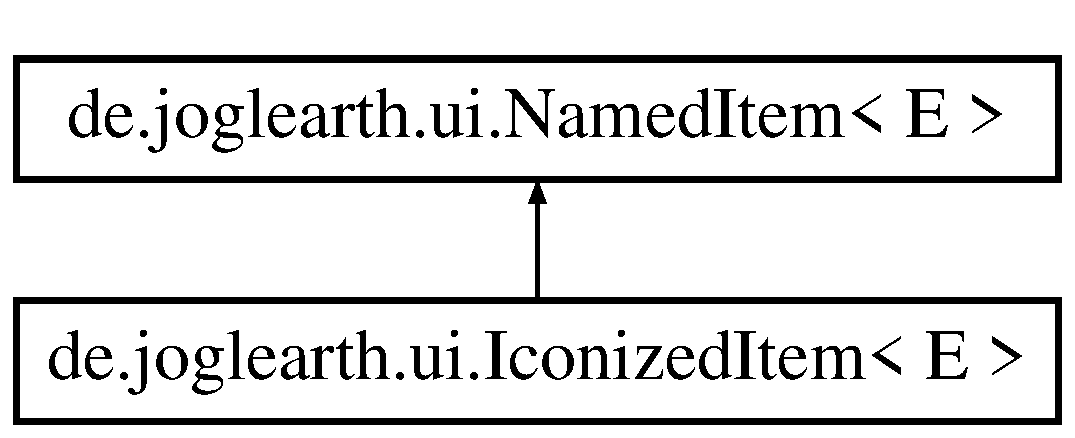
\includegraphics[height=2.000000cm]{classde_1_1joglearth_1_1ui_1_1_iconized_item_3_01_e_01_4}
\end{center}
\end{figure}
\subsection*{Öffentliche Methoden}
\begin{DoxyCompactItemize}
\item 
{\bfseries Iconized\-Item} (String name, Icon icon)\label{classde_1_1joglearth_1_1ui_1_1_iconized_item_3_01_e_01_4_a5136753310485d97e5fdb7ca28cccb9b}

\item 
{\bfseries Iconized\-Item} (String name, Icon icon, E value)\label{classde_1_1joglearth_1_1ui_1_1_iconized_item_3_01_e_01_4_a577dd778a6b303e1f82c78f81e5d2e26}

\item 
Icon {\bfseries get\-Icon} ()\label{classde_1_1joglearth_1_1ui_1_1_iconized_item_3_01_e_01_4_a595020855ba5c660c1f9925d293e8f08}

\end{DoxyCompactItemize}

\section{de.\-joglearth.\-ui.\-Icon\-List\-Cell\-Renderer$<$ E $>$ Klassenreferenz}
\label{classde_1_1joglearth_1_1ui_1_1_icon_list_cell_renderer_3_01_e_01_4}\index{de.\-joglearth.\-ui.\-Icon\-List\-Cell\-Renderer$<$ E $>$@{de.\-joglearth.\-ui.\-Icon\-List\-Cell\-Renderer$<$ E $>$}}
Klassendiagramm für de.\-joglearth.\-ui.\-Icon\-List\-Cell\-Renderer$<$ E $>$\-:\begin{figure}[H]
\begin{center}
\leavevmode
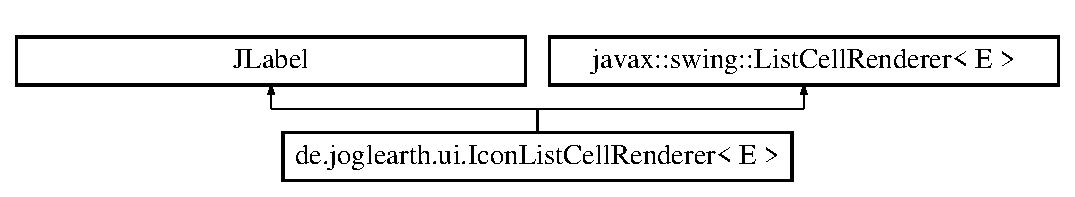
\includegraphics[height=2.000000cm]{classde_1_1joglearth_1_1ui_1_1_icon_list_cell_renderer_3_01_e_01_4}
\end{center}
\end{figure}
\subsection*{Öffentliche Methoden}
\begin{DoxyCompactItemize}
\item 
Component {\bfseries get\-List\-Cell\-Renderer\-Component} (J\-List$<$?extends E $>$ list, E value, int index, boolean is\-Selected, boolean cell\-Has\-Focus)\label{classde_1_1joglearth_1_1ui_1_1_icon_list_cell_renderer_3_01_e_01_4_ac613890106639359ca31c02e1ea0b09b}

\end{DoxyCompactItemize}

\section{de.\-joglearth.\-Jogl\-Earth Klassenreferenz}
\label{classde_1_1joglearth_1_1_jogl_earth}\index{de.\-joglearth.\-Jogl\-Earth@{de.\-joglearth.\-Jogl\-Earth}}
\subsection*{Öffentliche, statische Methoden}
\begin{DoxyCompactItemize}
\item 
static void {\bf main} (String[$\,$] args)
\end{DoxyCompactItemize}
\subsection*{Statische öffentliche Attribute}
\begin{DoxyCompactItemize}
\item 
static String {\bfseries P\-R\-O\-D\-U\-C\-T\-\_\-\-N\-A\-M\-E} = \char`\"{}Jogl Earth\char`\"{}\label{classde_1_1joglearth_1_1_jogl_earth_ac5eb2830ab27b702143759de25579f2b}

\item 
static String {\bfseries P\-R\-O\-D\-U\-C\-T\-\_\-\-V\-E\-R\-S\-I\-O\-N} = \char`\"{}0.\-1\char`\"{}\label{classde_1_1joglearth_1_1_jogl_earth_a989b83b1b12fa31076b4b6fe8dbff557}

\end{DoxyCompactItemize}


\subsection{Ausführliche Beschreibung}
Utility Class that contains the main method of \doxyref{Jogl\-Earth}{S.}{classde_1_1joglearth_1_1_jogl_earth}. 

\subsection{Dokumentation der Elementfunktionen}
\index{de\-::joglearth\-::\-Jogl\-Earth@{de\-::joglearth\-::\-Jogl\-Earth}!main@{main}}
\index{main@{main}!de::joglearth::JoglEarth@{de\-::joglearth\-::\-Jogl\-Earth}}
\subsubsection[{main}]{\setlength{\rightskip}{0pt plus 5cm}static void de.\-joglearth.\-Jogl\-Earth.\-main (
\begin{DoxyParamCaption}
\item[{String[$\,$]}]{args}
\end{DoxyParamCaption}
)\hspace{0.3cm}{\ttfamily [static]}}\label{classde_1_1joglearth_1_1_jogl_earth_a5ccf24fdd469fd100010c3778ad9cc31}
Initializes the \doxyref{Jogl\-Earth}{S.}{classde_1_1joglearth_1_1_jogl_earth} Application. There are no valid command line arguments. 
\begin{DoxyParams}{Parameter}
{\em args} & the command line arguments \\
\hline
\end{DoxyParams}

\section{de.\-joglearth.\-rendering.\-Level\-Of\-Detail Enum-\/\-Referenz}
\label{enumde_1_1joglearth_1_1rendering_1_1_level_of_detail}\index{de.\-joglearth.\-rendering.\-Level\-Of\-Detail@{de.\-joglearth.\-rendering.\-Level\-Of\-Detail}}
\subsection*{Öffentliche Attribute}
\begin{DoxyCompactItemize}
\item 
{\bfseries L\-O\-W}\label{enumde_1_1joglearth_1_1rendering_1_1_level_of_detail_aa31d78c2de0d480bb26f64494f50bc90}

\item 
{\bfseries M\-E\-D\-I\-U\-M}\label{enumde_1_1joglearth_1_1rendering_1_1_level_of_detail_a7f393f63040837c1cbdb72702734af23}

\item 
{\bfseries H\-I\-G\-H}\label{enumde_1_1joglearth_1_1rendering_1_1_level_of_detail_ae2979a91da15545e8392dcfea05cc126}

\end{DoxyCompactItemize}

\section{de.\-joglearth.\-surface.\-Location Klassenreferenz}
\label{classde_1_1joglearth_1_1surface_1_1_location}\index{de.\-joglearth.\-surface.\-Location@{de.\-joglearth.\-surface.\-Location}}
\subsection*{Öffentliche Methoden}
\begin{DoxyCompactItemize}
\item 
{\bf Location} ({\bf Geo\-Coordinates} {\bf point}, {\bf Location\-Type} {\bf type}, String {\bf details}, String {\bf name})
\end{DoxyCompactItemize}
\subsection*{Öffentliche Attribute}
\begin{DoxyCompactItemize}
\item 
{\bf Geo\-Coordinates} {\bf point}
\item 
{\bf Location\-Type} {\bf type}
\item 
String {\bf details}
\item 
String {\bf name}
\end{DoxyCompactItemize}


\subsection{Ausführliche Beschreibung}
Saves a points longitude, latitude and details. Is used by \doxyref{Location\-Manager}{S.}{classde_1_1joglearth_1_1surface_1_1_location_manager} to administer all kinds of points on a map. 

\subsection{Beschreibung der Konstruktoren und Destruktoren}
\index{de\-::joglearth\-::surface\-::\-Location@{de\-::joglearth\-::surface\-::\-Location}!Location@{Location}}
\index{Location@{Location}!de::joglearth::surface::Location@{de\-::joglearth\-::surface\-::\-Location}}
\subsubsection[{Location}]{\setlength{\rightskip}{0pt plus 5cm}de.\-joglearth.\-surface.\-Location.\-Location (
\begin{DoxyParamCaption}
\item[{{\bf Geo\-Coordinates}}]{point, }
\item[{{\bf Location\-Type}}]{type, }
\item[{String}]{details, }
\item[{String}]{name}
\end{DoxyParamCaption}
)}\label{classde_1_1joglearth_1_1surface_1_1_location_a9854c8c679be7283ce57751466cb9b62}
Assigns values to the local variables point, type and details.


\begin{DoxyParams}{Parameter}
{\em point} & The {\ttfamily Geo\-Coordinates} of a point \\
\hline
{\em type} & The {\ttfamily \doxyref{Location\-Type}{S.}{enumde_1_1joglearth_1_1surface_1_1_location_type}} of that specific point \\
\hline
{\em details} & A string containing gathered details about that point \\
\hline
{\em name} & A string containing the name of the {\ttfamily \doxyref{Location}{S.}{classde_1_1joglearth_1_1surface_1_1_location}} this should be used to display it in short form \\
\hline
\end{DoxyParams}


\subsection{Dokumentation der Datenelemente}
\index{de\-::joglearth\-::surface\-::\-Location@{de\-::joglearth\-::surface\-::\-Location}!details@{details}}
\index{details@{details}!de::joglearth::surface::Location@{de\-::joglearth\-::surface\-::\-Location}}
\subsubsection[{details}]{\setlength{\rightskip}{0pt plus 5cm}String de.\-joglearth.\-surface.\-Location.\-details}\label{classde_1_1joglearth_1_1surface_1_1_location_a97b49a9980f0a6efb44980fa499047e1}
Details of the location. \index{de\-::joglearth\-::surface\-::\-Location@{de\-::joglearth\-::surface\-::\-Location}!name@{name}}
\index{name@{name}!de::joglearth::surface::Location@{de\-::joglearth\-::surface\-::\-Location}}
\subsubsection[{name}]{\setlength{\rightskip}{0pt plus 5cm}String de.\-joglearth.\-surface.\-Location.\-name}\label{classde_1_1joglearth_1_1surface_1_1_location_aad9880d86e0d9e1bb062db174f6733a4}
Name of the location. \index{de\-::joglearth\-::surface\-::\-Location@{de\-::joglearth\-::surface\-::\-Location}!point@{point}}
\index{point@{point}!de::joglearth::surface::Location@{de\-::joglearth\-::surface\-::\-Location}}
\subsubsection[{point}]{\setlength{\rightskip}{0pt plus 5cm}{\bf Geo\-Coordinates} de.\-joglearth.\-surface.\-Location.\-point}\label{classde_1_1joglearth_1_1surface_1_1_location_ae13132f2481931170b4047309ad2b664}
Coordinates of the location. \index{de\-::joglearth\-::surface\-::\-Location@{de\-::joglearth\-::surface\-::\-Location}!type@{type}}
\index{type@{type}!de::joglearth::surface::Location@{de\-::joglearth\-::surface\-::\-Location}}
\subsubsection[{type}]{\setlength{\rightskip}{0pt plus 5cm}{\bf Location\-Type} de.\-joglearth.\-surface.\-Location.\-type}\label{classde_1_1joglearth_1_1surface_1_1_location_aa2a1b66692da2eea85a9f3a0e1f9f3ba}
Type of the location. 
\section{de.\-joglearth.\-ui.\-Location\-Edit\-Dialog Klassenreferenz}
\label{classde_1_1joglearth_1_1ui_1_1_location_edit_dialog}\index{de.\-joglearth.\-ui.\-Location\-Edit\-Dialog@{de.\-joglearth.\-ui.\-Location\-Edit\-Dialog}}


Abgeleitet von J\-Dialog.

\subsection*{Öffentliche Methoden}
\begin{DoxyCompactItemize}
\item 
{\bf Location\-Edit\-Dialog} ({\bf Location} location)
\end{DoxyCompactItemize}
\subsection*{Öffentliche, statische Methoden}
\begin{DoxyCompactItemize}
\item 
static void {\bfseries main} (String[$\,$] args)\label{classde_1_1joglearth_1_1ui_1_1_location_edit_dialog_aead6ae48da94fe7e0bf9d8a0477f59b2}

\end{DoxyCompactItemize}


\subsection{Ausführliche Beschreibung}
Dialog for entering information about a location. You can add a {\ttfamily Window\-Listener} to this dialog reaction to it closing. The given {\ttfamily Location} object will be manipulated before closing to represent the users input. 

\subsection{Beschreibung der Konstruktoren und Destruktoren}
\index{de\-::joglearth\-::ui\-::\-Location\-Edit\-Dialog@{de\-::joglearth\-::ui\-::\-Location\-Edit\-Dialog}!Location\-Edit\-Dialog@{Location\-Edit\-Dialog}}
\index{Location\-Edit\-Dialog@{Location\-Edit\-Dialog}!de::joglearth::ui::LocationEditDialog@{de\-::joglearth\-::ui\-::\-Location\-Edit\-Dialog}}
\subsubsection[{Location\-Edit\-Dialog}]{\setlength{\rightskip}{0pt plus 5cm}de.\-joglearth.\-ui.\-Location\-Edit\-Dialog.\-Location\-Edit\-Dialog (
\begin{DoxyParamCaption}
\item[{{\bf Location}}]{location}
\end{DoxyParamCaption}
)}\label{classde_1_1joglearth_1_1ui_1_1_location_edit_dialog_afedcdd11e1eeee316b0cd6b0447e58f3}
Create the dialog for entering information about a location.


\begin{DoxyParams}{Parameter}
{\em location} & The {\ttfamily Location} object will be changed before closing \\
\hline
\end{DoxyParams}

\section{de.\-joglearth.\-surface.\-Location\-Listener Schnittstellenreferenz}
\label{interfacede_1_1joglearth_1_1surface_1_1_location_listener}\index{de.\-joglearth.\-surface.\-Location\-Listener@{de.\-joglearth.\-surface.\-Location\-Listener}}


Basisklasse für de.\-joglearth.\-ui.\-Main\-Window.\-U\-I\-Location\-Listener.

\subsection*{Öffentliche Methoden}
\begin{DoxyCompactItemize}
\item 
void {\bf search\-Results\-Available} (Collection$<$ {\bf Location} $>$ results)
\end{DoxyCompactItemize}


\subsection{Ausführliche Beschreibung}
Classes implementing this interface receive asynchronous answers from the \doxyref{de.\-joglearth.\-surface.\-Location\-Mananger}{S.}{} such as search results. 

\subsection{Dokumentation der Elementfunktionen}
\index{de\-::joglearth\-::surface\-::\-Location\-Listener@{de\-::joglearth\-::surface\-::\-Location\-Listener}!search\-Results\-Available@{search\-Results\-Available}}
\index{search\-Results\-Available@{search\-Results\-Available}!de::joglearth::surface::LocationListener@{de\-::joglearth\-::surface\-::\-Location\-Listener}}
\subsubsection[{search\-Results\-Available}]{\setlength{\rightskip}{0pt plus 5cm}void de.\-joglearth.\-surface.\-Location\-Listener.\-search\-Results\-Available (
\begin{DoxyParamCaption}
\item[{Collection$<$ {\bf Location} $>$}]{results}
\end{DoxyParamCaption}
)}\label{interfacede_1_1joglearth_1_1surface_1_1_location_listener_a50be5db98471c99d17d39432b8588aad}
Is called as a notification that the results are available simultaneously to a \doxyref{Location}{S.}{classde_1_1joglearth_1_1surface_1_1_location} collection containing the results.


\begin{DoxyParams}{Parameter}
{\em results} & A collection of {\ttfamily Locations} with results of the search \\
\hline
\end{DoxyParams}

\section{de.\-joglearth.\-surface.\-Location\-Manager \-Klassenreferenz}
\label{classde_1_1joglearth_1_1surface_1_1_location_manager}\index{de.\-joglearth.\-surface.\-Location\-Manager@{de.\-joglearth.\-surface.\-Location\-Manager}}
\-Klassendiagramm für de.\-joglearth.\-surface.\-Location\-Manager\-:\begin{figure}[H]
\begin{center}
\leavevmode
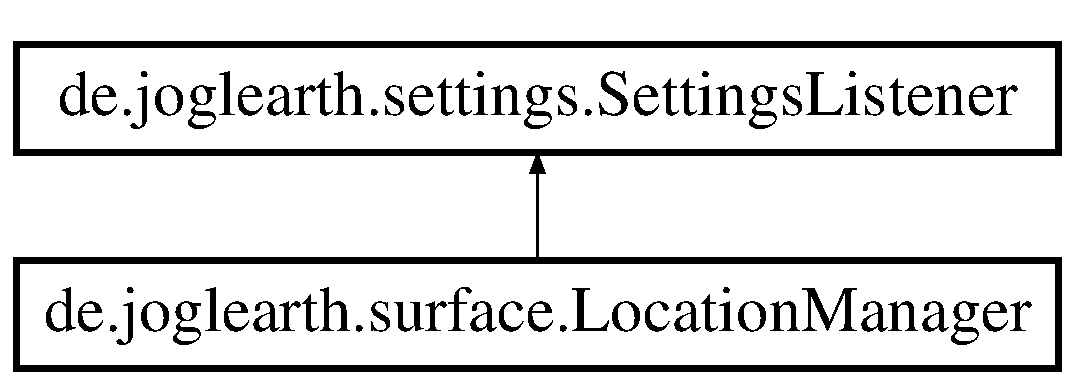
\includegraphics[height=2.000000cm]{classde_1_1joglearth_1_1surface_1_1_location_manager}
\end{center}
\end{figure}
\subsection*{Öffentliche \-Methoden}
\begin{DoxyCompactItemize}
\item 
{\bf \-Location\-Manager} ()
\item 
void {\bf show\-Location} ({\bf \-Location} location, boolean show)
\item 
void {\bf search\-Global} (\-String query)
\item 
void {\bf search\-Local} (\-String query, {\bf \-Tile}[$\,$] area)
\item 
{\bf \-Location} {\bf get\-Details} ({\bf \-Screen\-Coordinates} coordinates)
\item 
void {\bf settings\-Changed} (\-String key, \-Object val\-Old, \-Object val\-New)
\item 
void {\bf add\-Surface\-Listener} ({\bf \-Surface\-Listener} l)
\item 
void {\bf remove\-Surface\-Listener} ({\bf \-Surface\-Listener} l)
\item 
void {\bf add\-Location\-Listener} ({\bf \-Location\-Listener} l)
\item 
void {\bf remove\-Location\-Listener} ({\bf \-Location\-Listener} l)
\end{DoxyCompactItemize}


\subsection{\-Ausführliche \-Beschreibung}
\-Administers the visibility of particular points gathered from \doxyref{\-Overpass\-Source}{\-S.}{} and \doxyref{\-Nominatim\-Source}{\-S.}{}, and user marks from \doxyref{\-Settings}{\-S.}{}. 

\subsection{\-Beschreibung der \-Konstruktoren und \-Destruktoren}
\index{de\-::joglearth\-::surface\-::\-Location\-Manager@{de\-::joglearth\-::surface\-::\-Location\-Manager}!\-Location\-Manager@{\-Location\-Manager}}
\index{\-Location\-Manager@{\-Location\-Manager}!de::joglearth::surface::LocationManager@{de\-::joglearth\-::surface\-::\-Location\-Manager}}
\subsubsection[{\-Location\-Manager}]{\setlength{\rightskip}{0pt plus 5cm}{\bf de.\-joglearth.\-surface.\-Location\-Manager.\-Location\-Manager} (
\begin{DoxyParamCaption}
{}
\end{DoxyParamCaption}
)}\label{classde_1_1joglearth_1_1surface_1_1_location_manager_adfcd05b2a4cdbbccec1d664c8535dc00}
\-Constructor. \-Initializes the \doxyref{\-Location\-Manager}{\-S.}{classde_1_1joglearth_1_1surface_1_1_location_manager} and its underlying caches. 

\subsection{\-Dokumentation der \-Elementfunktionen}
\index{de\-::joglearth\-::surface\-::\-Location\-Manager@{de\-::joglearth\-::surface\-::\-Location\-Manager}!add\-Location\-Listener@{add\-Location\-Listener}}
\index{add\-Location\-Listener@{add\-Location\-Listener}!de::joglearth::surface::LocationManager@{de\-::joglearth\-::surface\-::\-Location\-Manager}}
\subsubsection[{add\-Location\-Listener}]{\setlength{\rightskip}{0pt plus 5cm}void {\bf de.\-joglearth.\-surface.\-Location\-Manager.\-add\-Location\-Listener} (
\begin{DoxyParamCaption}
\item[{{\bf \-Location\-Listener}}]{l}
\end{DoxyParamCaption}
)}\label{classde_1_1joglearth_1_1surface_1_1_location_manager_aaf3939f788ea9bffd8f188c429f2b796}
\-Adds a new \doxyref{\-Location\-Listener}{\-S.}{interfacede_1_1joglearth_1_1surface_1_1_location_listener} that is called when the search results are available.


\begin{DoxyParams}{\-Parameter}
{\em l} & \-The new {\ttfamily \doxyref{\-Location\-Listener}{\-S.}{interfacede_1_1joglearth_1_1surface_1_1_location_listener}} \\
\hline
\end{DoxyParams}
\index{de\-::joglearth\-::surface\-::\-Location\-Manager@{de\-::joglearth\-::surface\-::\-Location\-Manager}!add\-Surface\-Listener@{add\-Surface\-Listener}}
\index{add\-Surface\-Listener@{add\-Surface\-Listener}!de::joglearth::surface::LocationManager@{de\-::joglearth\-::surface\-::\-Location\-Manager}}
\subsubsection[{add\-Surface\-Listener}]{\setlength{\rightskip}{0pt plus 5cm}void {\bf de.\-joglearth.\-surface.\-Location\-Manager.\-add\-Surface\-Listener} (
\begin{DoxyParamCaption}
\item[{{\bf \-Surface\-Listener}}]{l}
\end{DoxyParamCaption}
)}\label{classde_1_1joglearth_1_1surface_1_1_location_manager_a4fb6df51c96474cb8ab082f6d41e2a29}
\-Adds a new \doxyref{\-Surface\-Listener}{\-S.}{interfacede_1_1joglearth_1_1surface_1_1_surface_listener} that is called on every change of the surface.


\begin{DoxyParams}{\-Parameter}
{\em l} & \-The new {\ttfamily \doxyref{\-Surface\-Listener}{\-S.}{interfacede_1_1joglearth_1_1surface_1_1_surface_listener}} \\
\hline
\end{DoxyParams}
\index{de\-::joglearth\-::surface\-::\-Location\-Manager@{de\-::joglearth\-::surface\-::\-Location\-Manager}!get\-Details@{get\-Details}}
\index{get\-Details@{get\-Details}!de::joglearth::surface::LocationManager@{de\-::joglearth\-::surface\-::\-Location\-Manager}}
\subsubsection[{get\-Details}]{\setlength{\rightskip}{0pt plus 5cm}{\bf \-Location} {\bf de.\-joglearth.\-surface.\-Location\-Manager.\-get\-Details} (
\begin{DoxyParamCaption}
\item[{{\bf \-Screen\-Coordinates}}]{coordinates}
\end{DoxyParamCaption}
)}\label{classde_1_1joglearth_1_1surface_1_1_location_manager_a5a37434c3d2bfd665f9915dd9d1690c7}
\-Gets the details of a point with given \doxyref{\-Screen\-Coordinates}{\-S.}{}. \-To achieve that it asks the \doxyref{\-Request\-Distributor}{\-S.}{}.


\begin{DoxyParams}{\-Parameter}
{\em coordinates} & \-The {\ttfamily \-Screen\-Coordinates} of the point \\
\hline
\end{DoxyParams}
\begin{DoxyReturn}{\-Rückgabe}
\-The {\ttfamily \doxyref{\-Location}{\-S.}{classde_1_1joglearth_1_1surface_1_1_location}} with details that is located on the given point or a {\ttfamily \doxyref{\-Location}{\-S.}{classde_1_1joglearth_1_1surface_1_1_location}} without details if the details are not yet loaded. 
\end{DoxyReturn}
\index{de\-::joglearth\-::surface\-::\-Location\-Manager@{de\-::joglearth\-::surface\-::\-Location\-Manager}!remove\-Location\-Listener@{remove\-Location\-Listener}}
\index{remove\-Location\-Listener@{remove\-Location\-Listener}!de::joglearth::surface::LocationManager@{de\-::joglearth\-::surface\-::\-Location\-Manager}}
\subsubsection[{remove\-Location\-Listener}]{\setlength{\rightskip}{0pt plus 5cm}void {\bf de.\-joglearth.\-surface.\-Location\-Manager.\-remove\-Location\-Listener} (
\begin{DoxyParamCaption}
\item[{{\bf \-Location\-Listener}}]{l}
\end{DoxyParamCaption}
)}\label{classde_1_1joglearth_1_1surface_1_1_location_manager_a4e2c63aff73eb0e1d84a878d28ea4806}
\-Removes a specific \doxyref{\-Location\-Listener}{\-S.}{interfacede_1_1joglearth_1_1surface_1_1_location_listener}.


\begin{DoxyParams}{\-Parameter}
{\em l} & \-The {\ttfamily \doxyref{\-Location\-Listener}{\-S.}{interfacede_1_1joglearth_1_1surface_1_1_location_listener}} that should be removed \\
\hline
\end{DoxyParams}
\index{de\-::joglearth\-::surface\-::\-Location\-Manager@{de\-::joglearth\-::surface\-::\-Location\-Manager}!remove\-Surface\-Listener@{remove\-Surface\-Listener}}
\index{remove\-Surface\-Listener@{remove\-Surface\-Listener}!de::joglearth::surface::LocationManager@{de\-::joglearth\-::surface\-::\-Location\-Manager}}
\subsubsection[{remove\-Surface\-Listener}]{\setlength{\rightskip}{0pt plus 5cm}void {\bf de.\-joglearth.\-surface.\-Location\-Manager.\-remove\-Surface\-Listener} (
\begin{DoxyParamCaption}
\item[{{\bf \-Surface\-Listener}}]{l}
\end{DoxyParamCaption}
)}\label{classde_1_1joglearth_1_1surface_1_1_location_manager_ad789dd615685883b93701d8a443d5eab}
\-Removes a specific \doxyref{\-Surface\-Listener}{\-S.}{interfacede_1_1joglearth_1_1surface_1_1_surface_listener}.


\begin{DoxyParams}{\-Parameter}
{\em l} & \-The {\ttfamily \doxyref{\-Surface\-Listener}{\-S.}{interfacede_1_1joglearth_1_1surface_1_1_surface_listener}} that should be removed \\
\hline
\end{DoxyParams}
\index{de\-::joglearth\-::surface\-::\-Location\-Manager@{de\-::joglearth\-::surface\-::\-Location\-Manager}!search\-Global@{search\-Global}}
\index{search\-Global@{search\-Global}!de::joglearth::surface::LocationManager@{de\-::joglearth\-::surface\-::\-Location\-Manager}}
\subsubsection[{search\-Global}]{\setlength{\rightskip}{0pt plus 5cm}void {\bf de.\-joglearth.\-surface.\-Location\-Manager.\-search\-Global} (
\begin{DoxyParamCaption}
\item[{\-String}]{query}
\end{DoxyParamCaption}
)}\label{classde_1_1joglearth_1_1surface_1_1_location_manager_ab63d6eadbd5c39558bbac1e81409b902}
\-Searches on the whole globe/map after a query string.


\begin{DoxyParams}{\-Parameter}
{\em query} & \-The query string \\
\hline
\end{DoxyParams}
\index{de\-::joglearth\-::surface\-::\-Location\-Manager@{de\-::joglearth\-::surface\-::\-Location\-Manager}!search\-Local@{search\-Local}}
\index{search\-Local@{search\-Local}!de::joglearth::surface::LocationManager@{de\-::joglearth\-::surface\-::\-Location\-Manager}}
\subsubsection[{search\-Local}]{\setlength{\rightskip}{0pt plus 5cm}void {\bf de.\-joglearth.\-surface.\-Location\-Manager.\-search\-Local} (
\begin{DoxyParamCaption}
\item[{\-String}]{query, }
\item[{{\bf \-Tile}[$\,$]}]{area}
\end{DoxyParamCaption}
)}\label{classde_1_1joglearth_1_1surface_1_1_location_manager_abd861424864158ced5760a5d74ceddd9}
\-Searches after a query string on the visible part of the map/globe.


\begin{DoxyParams}{\-Parameter}
{\em query} & \-The query string \\
\hline
{\em area} & \-An array of visible tiles where the search should be performed on \\
\hline
\end{DoxyParams}
\index{de\-::joglearth\-::surface\-::\-Location\-Manager@{de\-::joglearth\-::surface\-::\-Location\-Manager}!settings\-Changed@{settings\-Changed}}
\index{settings\-Changed@{settings\-Changed}!de::joglearth::surface::LocationManager@{de\-::joglearth\-::surface\-::\-Location\-Manager}}
\subsubsection[{settings\-Changed}]{\setlength{\rightskip}{0pt plus 5cm}void {\bf de.\-joglearth.\-surface.\-Location\-Manager.\-settings\-Changed} (
\begin{DoxyParamCaption}
\item[{\-String}]{key, }
\item[{\-Object}]{val\-Old, }
\item[{\-Object}]{val\-New}
\end{DoxyParamCaption}
)}\label{classde_1_1joglearth_1_1surface_1_1_location_manager_a5cb5a6e42aff0c82ee889c37ae72bfcc}
\-Invoked if a setting this listener has be registered on is changed.


\begin{DoxyParams}{\-Parameter}
{\em key} & \-The key of the changed setting \\
\hline
{\em val\-Old} & \-The old value of the setting, can be null if there wasn't any \\
\hline
{\em val\-New} & \-The new value of the setting, can be null \\
\hline
\end{DoxyParams}


\-Implementiert {\bf de.\-joglearth.\-settings.\-Settings\-Listener} \doxyref{}{\-S.}{interfacede_1_1joglearth_1_1settings_1_1_settings_listener_a77fca7f974574ac990a8ed54cb076aef}.

\index{de\-::joglearth\-::surface\-::\-Location\-Manager@{de\-::joglearth\-::surface\-::\-Location\-Manager}!show\-Location@{show\-Location}}
\index{show\-Location@{show\-Location}!de::joglearth::surface::LocationManager@{de\-::joglearth\-::surface\-::\-Location\-Manager}}
\subsubsection[{show\-Location}]{\setlength{\rightskip}{0pt plus 5cm}void {\bf de.\-joglearth.\-surface.\-Location\-Manager.\-show\-Location} (
\begin{DoxyParamCaption}
\item[{{\bf \-Location}}]{location, }
\item[{boolean}]{show}
\end{DoxyParamCaption}
)}\label{classde_1_1joglearth_1_1surface_1_1_location_manager_a1e143c25e71b58c056f22dbde5b55e64}
\-Changes the visibility of a given \doxyref{\-Location}{\-S.}{classde_1_1joglearth_1_1surface_1_1_location}.


\begin{DoxyParams}{\-Parameter}
{\em location} & \-The {\ttfamily \doxyref{\-Location}{\-S.}{classde_1_1joglearth_1_1surface_1_1_location}} that should be shown \\
\hline
{\em show} & \-Whether to show or hide the display \\
\hline
\end{DoxyParams}

\section{de.\-joglearth.\-surface.\-Location\-Type Enum-\/\-Referenz}
\label{enumde_1_1joglearth_1_1surface_1_1_location_type}\index{de.\-joglearth.\-surface.\-Location\-Type@{de.\-joglearth.\-surface.\-Location\-Type}}
\subsection*{Öffentliche Attribute}
\begin{DoxyCompactItemize}
\item 
{\bf R\-E\-S\-T\-A\-U\-R\-A\-N\-T}
\item 
{\bf N\-I\-G\-H\-T\-L\-I\-F\-E}
\item 
{\bf B\-A\-N\-K}
\item 
{\bf T\-O\-I\-L\-E\-T\-S}
\item 
{\bf G\-R\-O\-C\-E\-R\-Y\-\_\-\-S\-H\-O\-P\-S}
\item 
{\bf S\-H\-O\-P\-S}
\item 
{\bf A\-C\-T\-I\-V\-I\-T\-Y}
\item 
{\bf H\-I\-K\-I\-N\-G\-\_\-\-A\-N\-D\-\_\-\-C\-Y\-C\-L\-I\-N\-G}
\item 
{\bf E\-D\-U\-C\-A\-T\-I\-O\-N}
\item 
{\bf H\-E\-A\-L\-T\-H}
\item 
{\bf P\-O\-S\-T}
\item 
{\bf H\-O\-T\-E\-L\-S}
\item 
{\bf C\-I\-T\-Y}
\item 
{\bf T\-O\-W\-N}
\item 
{\bf V\-I\-L\-L\-A\-G\-E}
\item 
{\bf U\-S\-E\-R\-\_\-\-T\-A\-G}
\end{DoxyCompactItemize}


\subsection{Ausführliche Beschreibung}
Represents overlay types like P\-O\-Is, city names and points marked by the user. 

\subsection{Dokumentation der Datenelemente}
\index{de\-::joglearth\-::surface\-::\-Location\-Type@{de\-::joglearth\-::surface\-::\-Location\-Type}!A\-C\-T\-I\-V\-I\-T\-Y@{A\-C\-T\-I\-V\-I\-T\-Y}}
\index{A\-C\-T\-I\-V\-I\-T\-Y@{A\-C\-T\-I\-V\-I\-T\-Y}!de::joglearth::surface::LocationType@{de\-::joglearth\-::surface\-::\-Location\-Type}}
\subsubsection[{A\-C\-T\-I\-V\-I\-T\-Y}]{\setlength{\rightskip}{0pt plus 5cm}de.\-joglearth.\-surface.\-Location\-Type.\-A\-C\-T\-I\-V\-I\-T\-Y}\label{enumde_1_1joglearth_1_1surface_1_1_location_type_a28340970988e4afac0935d274f8db994}
Returns spare-\/time activities like amusement parks or museums, places for picnics and lookouts. \index{de\-::joglearth\-::surface\-::\-Location\-Type@{de\-::joglearth\-::surface\-::\-Location\-Type}!B\-A\-N\-K@{B\-A\-N\-K}}
\index{B\-A\-N\-K@{B\-A\-N\-K}!de::joglearth::surface::LocationType@{de\-::joglearth\-::surface\-::\-Location\-Type}}
\subsubsection[{B\-A\-N\-K}]{\setlength{\rightskip}{0pt plus 5cm}de.\-joglearth.\-surface.\-Location\-Type.\-B\-A\-N\-K}\label{enumde_1_1joglearth_1_1surface_1_1_location_type_a64d4431c5b47f2b9144cd6f9668688d9}
Returns banks. \index{de\-::joglearth\-::surface\-::\-Location\-Type@{de\-::joglearth\-::surface\-::\-Location\-Type}!C\-I\-T\-Y@{C\-I\-T\-Y}}
\index{C\-I\-T\-Y@{C\-I\-T\-Y}!de::joglearth::surface::LocationType@{de\-::joglearth\-::surface\-::\-Location\-Type}}
\subsubsection[{C\-I\-T\-Y}]{\setlength{\rightskip}{0pt plus 5cm}de.\-joglearth.\-surface.\-Location\-Type.\-C\-I\-T\-Y}\label{enumde_1_1joglearth_1_1surface_1_1_location_type_a88e58e3621d44e143dfecdfb6acb90f4}
Returns a city. \index{de\-::joglearth\-::surface\-::\-Location\-Type@{de\-::joglearth\-::surface\-::\-Location\-Type}!E\-D\-U\-C\-A\-T\-I\-O\-N@{E\-D\-U\-C\-A\-T\-I\-O\-N}}
\index{E\-D\-U\-C\-A\-T\-I\-O\-N@{E\-D\-U\-C\-A\-T\-I\-O\-N}!de::joglearth::surface::LocationType@{de\-::joglearth\-::surface\-::\-Location\-Type}}
\subsubsection[{E\-D\-U\-C\-A\-T\-I\-O\-N}]{\setlength{\rightskip}{0pt plus 5cm}de.\-joglearth.\-surface.\-Location\-Type.\-E\-D\-U\-C\-A\-T\-I\-O\-N}\label{enumde_1_1joglearth_1_1surface_1_1_location_type_a086c59190e0cf154fceb2da543fd7d54}
Returns educational institutions. \index{de\-::joglearth\-::surface\-::\-Location\-Type@{de\-::joglearth\-::surface\-::\-Location\-Type}!G\-R\-O\-C\-E\-R\-Y\-\_\-\-S\-H\-O\-P\-S@{G\-R\-O\-C\-E\-R\-Y\-\_\-\-S\-H\-O\-P\-S}}
\index{G\-R\-O\-C\-E\-R\-Y\-\_\-\-S\-H\-O\-P\-S@{G\-R\-O\-C\-E\-R\-Y\-\_\-\-S\-H\-O\-P\-S}!de::joglearth::surface::LocationType@{de\-::joglearth\-::surface\-::\-Location\-Type}}
\subsubsection[{G\-R\-O\-C\-E\-R\-Y\-\_\-\-S\-H\-O\-P\-S}]{\setlength{\rightskip}{0pt plus 5cm}de.\-joglearth.\-surface.\-Location\-Type.\-G\-R\-O\-C\-E\-R\-Y\-\_\-\-S\-H\-O\-P\-S}\label{enumde_1_1joglearth_1_1surface_1_1_location_type_a8c74d64e31a2e3f52a1005227782330b}
Returns supermarkets, bakeries, butchers and drug stores. \index{de\-::joglearth\-::surface\-::\-Location\-Type@{de\-::joglearth\-::surface\-::\-Location\-Type}!H\-E\-A\-L\-T\-H@{H\-E\-A\-L\-T\-H}}
\index{H\-E\-A\-L\-T\-H@{H\-E\-A\-L\-T\-H}!de::joglearth::surface::LocationType@{de\-::joglearth\-::surface\-::\-Location\-Type}}
\subsubsection[{H\-E\-A\-L\-T\-H}]{\setlength{\rightskip}{0pt plus 5cm}de.\-joglearth.\-surface.\-Location\-Type.\-H\-E\-A\-L\-T\-H}\label{enumde_1_1joglearth_1_1surface_1_1_location_type_a6874f836540b65238f8bf98e0a929f7e}
Returns doctors, hospitals, chemists and drug stores. \index{de\-::joglearth\-::surface\-::\-Location\-Type@{de\-::joglearth\-::surface\-::\-Location\-Type}!H\-I\-K\-I\-N\-G\-\_\-\-A\-N\-D\-\_\-\-C\-Y\-C\-L\-I\-N\-G@{H\-I\-K\-I\-N\-G\-\_\-\-A\-N\-D\-\_\-\-C\-Y\-C\-L\-I\-N\-G}}
\index{H\-I\-K\-I\-N\-G\-\_\-\-A\-N\-D\-\_\-\-C\-Y\-C\-L\-I\-N\-G@{H\-I\-K\-I\-N\-G\-\_\-\-A\-N\-D\-\_\-\-C\-Y\-C\-L\-I\-N\-G}!de::joglearth::surface::LocationType@{de\-::joglearth\-::surface\-::\-Location\-Type}}
\subsubsection[{H\-I\-K\-I\-N\-G\-\_\-\-A\-N\-D\-\_\-\-C\-Y\-C\-L\-I\-N\-G}]{\setlength{\rightskip}{0pt plus 5cm}de.\-joglearth.\-surface.\-Location\-Type.\-H\-I\-K\-I\-N\-G\-\_\-\-A\-N\-D\-\_\-\-C\-Y\-C\-L\-I\-N\-G}\label{enumde_1_1joglearth_1_1surface_1_1_location_type_a41999573598055d629bdbf47593ec7d6}
Returns outdoor pursuits for bikers and hikers like picnic places and lookouts, benches, rubbish bins and bike shops. \index{de\-::joglearth\-::surface\-::\-Location\-Type@{de\-::joglearth\-::surface\-::\-Location\-Type}!H\-O\-T\-E\-L\-S@{H\-O\-T\-E\-L\-S}}
\index{H\-O\-T\-E\-L\-S@{H\-O\-T\-E\-L\-S}!de::joglearth::surface::LocationType@{de\-::joglearth\-::surface\-::\-Location\-Type}}
\subsubsection[{H\-O\-T\-E\-L\-S}]{\setlength{\rightskip}{0pt plus 5cm}de.\-joglearth.\-surface.\-Location\-Type.\-H\-O\-T\-E\-L\-S}\label{enumde_1_1joglearth_1_1surface_1_1_location_type_a39659f87bbe5dfb75b466fadd1dc79f0}
Returns hotels and bed and breakfast places. \index{de\-::joglearth\-::surface\-::\-Location\-Type@{de\-::joglearth\-::surface\-::\-Location\-Type}!N\-I\-G\-H\-T\-L\-I\-F\-E@{N\-I\-G\-H\-T\-L\-I\-F\-E}}
\index{N\-I\-G\-H\-T\-L\-I\-F\-E@{N\-I\-G\-H\-T\-L\-I\-F\-E}!de::joglearth::surface::LocationType@{de\-::joglearth\-::surface\-::\-Location\-Type}}
\subsubsection[{N\-I\-G\-H\-T\-L\-I\-F\-E}]{\setlength{\rightskip}{0pt plus 5cm}de.\-joglearth.\-surface.\-Location\-Type.\-N\-I\-G\-H\-T\-L\-I\-F\-E}\label{enumde_1_1joglearth_1_1surface_1_1_location_type_a736c4265079449978596e044fe09e12a}
Returns bars, clubs, cinemas and solaria (tanning booths). \index{de\-::joglearth\-::surface\-::\-Location\-Type@{de\-::joglearth\-::surface\-::\-Location\-Type}!P\-O\-S\-T@{P\-O\-S\-T}}
\index{P\-O\-S\-T@{P\-O\-S\-T}!de::joglearth::surface::LocationType@{de\-::joglearth\-::surface\-::\-Location\-Type}}
\subsubsection[{P\-O\-S\-T}]{\setlength{\rightskip}{0pt plus 5cm}de.\-joglearth.\-surface.\-Location\-Type.\-P\-O\-S\-T}\label{enumde_1_1joglearth_1_1surface_1_1_location_type_a22abc1195ef2e8f2914ba0a5158ee350}
Returns post offices, mailboxes and freight stations. \index{de\-::joglearth\-::surface\-::\-Location\-Type@{de\-::joglearth\-::surface\-::\-Location\-Type}!R\-E\-S\-T\-A\-U\-R\-A\-N\-T@{R\-E\-S\-T\-A\-U\-R\-A\-N\-T}}
\index{R\-E\-S\-T\-A\-U\-R\-A\-N\-T@{R\-E\-S\-T\-A\-U\-R\-A\-N\-T}!de::joglearth::surface::LocationType@{de\-::joglearth\-::surface\-::\-Location\-Type}}
\subsubsection[{R\-E\-S\-T\-A\-U\-R\-A\-N\-T}]{\setlength{\rightskip}{0pt plus 5cm}de.\-joglearth.\-surface.\-Location\-Type.\-R\-E\-S\-T\-A\-U\-R\-A\-N\-T}\label{enumde_1_1joglearth_1_1surface_1_1_location_type_ad903ebec28ff7e057351456986386318}
Returns cafes, restaurants and beer gardens. \index{de\-::joglearth\-::surface\-::\-Location\-Type@{de\-::joglearth\-::surface\-::\-Location\-Type}!S\-H\-O\-P\-S@{S\-H\-O\-P\-S}}
\index{S\-H\-O\-P\-S@{S\-H\-O\-P\-S}!de::joglearth::surface::LocationType@{de\-::joglearth\-::surface\-::\-Location\-Type}}
\subsubsection[{S\-H\-O\-P\-S}]{\setlength{\rightskip}{0pt plus 5cm}de.\-joglearth.\-surface.\-Location\-Type.\-S\-H\-O\-P\-S}\label{enumde_1_1joglearth_1_1surface_1_1_location_type_a9b23db87e93e3d314054967a608d8e51}
Returns a variety of shops. \index{de\-::joglearth\-::surface\-::\-Location\-Type@{de\-::joglearth\-::surface\-::\-Location\-Type}!T\-O\-I\-L\-E\-T\-S@{T\-O\-I\-L\-E\-T\-S}}
\index{T\-O\-I\-L\-E\-T\-S@{T\-O\-I\-L\-E\-T\-S}!de::joglearth::surface::LocationType@{de\-::joglearth\-::surface\-::\-Location\-Type}}
\subsubsection[{T\-O\-I\-L\-E\-T\-S}]{\setlength{\rightskip}{0pt plus 5cm}de.\-joglearth.\-surface.\-Location\-Type.\-T\-O\-I\-L\-E\-T\-S}\label{enumde_1_1joglearth_1_1surface_1_1_location_type_a858d26e00ba81fb9df0f5c50a528528f}
Returns public toilets. \index{de\-::joglearth\-::surface\-::\-Location\-Type@{de\-::joglearth\-::surface\-::\-Location\-Type}!T\-O\-W\-N@{T\-O\-W\-N}}
\index{T\-O\-W\-N@{T\-O\-W\-N}!de::joglearth::surface::LocationType@{de\-::joglearth\-::surface\-::\-Location\-Type}}
\subsubsection[{T\-O\-W\-N}]{\setlength{\rightskip}{0pt plus 5cm}de.\-joglearth.\-surface.\-Location\-Type.\-T\-O\-W\-N}\label{enumde_1_1joglearth_1_1surface_1_1_location_type_a7ba1bddcaa4afb274dc98310501a11d8}
Returns a town. \index{de\-::joglearth\-::surface\-::\-Location\-Type@{de\-::joglearth\-::surface\-::\-Location\-Type}!U\-S\-E\-R\-\_\-\-T\-A\-G@{U\-S\-E\-R\-\_\-\-T\-A\-G}}
\index{U\-S\-E\-R\-\_\-\-T\-A\-G@{U\-S\-E\-R\-\_\-\-T\-A\-G}!de::joglearth::surface::LocationType@{de\-::joglearth\-::surface\-::\-Location\-Type}}
\subsubsection[{U\-S\-E\-R\-\_\-\-T\-A\-G}]{\setlength{\rightskip}{0pt plus 5cm}de.\-joglearth.\-surface.\-Location\-Type.\-U\-S\-E\-R\-\_\-\-T\-A\-G}\label{enumde_1_1joglearth_1_1surface_1_1_location_type_a21a7496394cbc7e7865d5b9580805210}
Returns a point marked by the user. \index{de\-::joglearth\-::surface\-::\-Location\-Type@{de\-::joglearth\-::surface\-::\-Location\-Type}!V\-I\-L\-L\-A\-G\-E@{V\-I\-L\-L\-A\-G\-E}}
\index{V\-I\-L\-L\-A\-G\-E@{V\-I\-L\-L\-A\-G\-E}!de::joglearth::surface::LocationType@{de\-::joglearth\-::surface\-::\-Location\-Type}}
\subsubsection[{V\-I\-L\-L\-A\-G\-E}]{\setlength{\rightskip}{0pt plus 5cm}de.\-joglearth.\-surface.\-Location\-Type.\-V\-I\-L\-L\-A\-G\-E}\label{enumde_1_1joglearth_1_1surface_1_1_location_type_a7ec83c09367dd0fbdb2dba1d38138625}
Returns a village. 
\section{de.\-joglearth.\-ui.\-Main\-Window Klassenreferenz}
\label{classde_1_1joglearth_1_1ui_1_1_main_window}\index{de.\-joglearth.\-ui.\-Main\-Window@{de.\-joglearth.\-ui.\-Main\-Window}}
Klassendiagramm für de.\-joglearth.\-ui.\-Main\-Window\-:\begin{figure}[H]
\begin{center}
\leavevmode
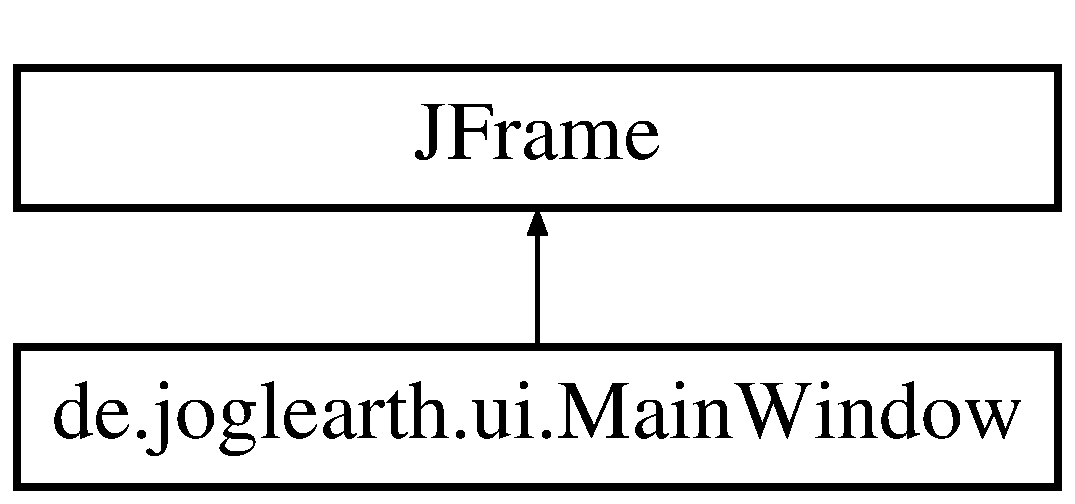
\includegraphics[height=2.000000cm]{classde_1_1joglearth_1_1ui_1_1_main_window}
\end{center}
\end{figure}
\subsection*{Öffentliche Methoden}
\begin{DoxyCompactItemize}
\item 
{\bf Main\-Window} (final {\bf Location\-Manager} location\-Manager, final {\bf Camera} camera)
\item 
final G\-L\-Canvas {\bf get\-G\-L\-Canvas} ()
\end{DoxyCompactItemize}
\subsection*{Öffentliche, statische Methoden}
\begin{DoxyCompactItemize}
\item 
static void {\bf main} (String[$\,$] args)
\end{DoxyCompactItemize}


\subsection{Ausführliche Beschreibung}
This class is used to create the main ui window for joglearth. 

\subsection{Beschreibung der Konstruktoren und Destruktoren}
\index{de\-::joglearth\-::ui\-::\-Main\-Window@{de\-::joglearth\-::ui\-::\-Main\-Window}!Main\-Window@{Main\-Window}}
\index{Main\-Window@{Main\-Window}!de::joglearth::ui::MainWindow@{de\-::joglearth\-::ui\-::\-Main\-Window}}
\subsubsection[{Main\-Window}]{\setlength{\rightskip}{0pt plus 5cm}de.\-joglearth.\-ui.\-Main\-Window.\-Main\-Window (
\begin{DoxyParamCaption}
\item[{final {\bf Location\-Manager}}]{location\-Manager, }
\item[{final {\bf Camera}}]{camera}
\end{DoxyParamCaption}
)}\label{classde_1_1joglearth_1_1ui_1_1_main_window_ad4f0ff0452ee258031d69bd1704f842b}
Constructor to create he window out of a given \doxyref{Location\-Manager}{S.}{} and \doxyref{Camera}{S.}{}.


\begin{DoxyParams}{Parameter}
{\em location\-Manager} & the {\ttfamily Location\-Manager} used by this window \\
\hline
{\em camera} & the {\ttfamily Camera} used by this window \\
\hline
\end{DoxyParams}


\subsection{Dokumentation der Elementfunktionen}
\index{de\-::joglearth\-::ui\-::\-Main\-Window@{de\-::joglearth\-::ui\-::\-Main\-Window}!get\-G\-L\-Canvas@{get\-G\-L\-Canvas}}
\index{get\-G\-L\-Canvas@{get\-G\-L\-Canvas}!de::joglearth::ui::MainWindow@{de\-::joglearth\-::ui\-::\-Main\-Window}}
\subsubsection[{get\-G\-L\-Canvas}]{\setlength{\rightskip}{0pt plus 5cm}final G\-L\-Canvas de.\-joglearth.\-ui.\-Main\-Window.\-get\-G\-L\-Canvas (
\begin{DoxyParamCaption}
{}
\end{DoxyParamCaption}
)}\label{classde_1_1joglearth_1_1ui_1_1_main_window_a3d82ce375de7cdd88323b6f1cd9bda05}
Gets the {\ttfamily G\-L\-Canvas} that is displayed in the left half of the window.

\begin{DoxyReturn}{Rückgabe}
the G\-L\-Canvas used in this window 
\end{DoxyReturn}
\index{de\-::joglearth\-::ui\-::\-Main\-Window@{de\-::joglearth\-::ui\-::\-Main\-Window}!main@{main}}
\index{main@{main}!de::joglearth::ui::MainWindow@{de\-::joglearth\-::ui\-::\-Main\-Window}}
\subsubsection[{main}]{\setlength{\rightskip}{0pt plus 5cm}static void de.\-joglearth.\-ui.\-Main\-Window.\-main (
\begin{DoxyParamCaption}
\item[{String[$\,$]}]{args}
\end{DoxyParamCaption}
)\hspace{0.3cm}{\ttfamily [static]}}\label{classde_1_1joglearth_1_1ui_1_1_main_window_a6655d08b45d09fdfa1b5229560e79608}
Launch the application. 
\section{de.\-joglearth.\-surface.\-Map\-Layout Enum-\/\-Referenz}
\label{enumde_1_1joglearth_1_1surface_1_1_map_layout}\index{de.\-joglearth.\-surface.\-Map\-Layout@{de.\-joglearth.\-surface.\-Map\-Layout}}
\subsection*{Öffentliche Attribute}
\begin{DoxyCompactItemize}
\item 
{\bf S\-I\-N\-G\-L\-E}
\item 
{\bf T\-I\-L\-E\-D}
\end{DoxyCompactItemize}


\subsection{Ausführliche Beschreibung}
Enumerates types of map texture layouts handled by a \doxyref{de.\-joglearth.\-rendering.\-Renderer}{S.}{classde_1_1joglearth_1_1rendering_1_1_renderer}. 

\subsection{Dokumentation der Datenelemente}
\index{de\-::joglearth\-::surface\-::\-Map\-Layout@{de\-::joglearth\-::surface\-::\-Map\-Layout}!S\-I\-N\-G\-L\-E@{S\-I\-N\-G\-L\-E}}
\index{S\-I\-N\-G\-L\-E@{S\-I\-N\-G\-L\-E}!de::joglearth::surface::MapLayout@{de\-::joglearth\-::surface\-::\-Map\-Layout}}
\subsubsection[{S\-I\-N\-G\-L\-E}]{\setlength{\rightskip}{0pt plus 5cm}de.\-joglearth.\-surface.\-Map\-Layout.\-S\-I\-N\-G\-L\-E}\label{enumde_1_1joglearth_1_1surface_1_1_map_layout_aaf8ac710f3eea275826fd076c50fc8d7}
The map is a single texture covering the whole earth. A single sphere or plane must be rendered to display it. \index{de\-::joglearth\-::surface\-::\-Map\-Layout@{de\-::joglearth\-::surface\-::\-Map\-Layout}!T\-I\-L\-E\-D@{T\-I\-L\-E\-D}}
\index{T\-I\-L\-E\-D@{T\-I\-L\-E\-D}!de::joglearth::surface::MapLayout@{de\-::joglearth\-::surface\-::\-Map\-Layout}}
\subsubsection[{T\-I\-L\-E\-D}]{\setlength{\rightskip}{0pt plus 5cm}de.\-joglearth.\-surface.\-Map\-Layout.\-T\-I\-L\-E\-D}\label{enumde_1_1joglearth_1_1surface_1_1_map_layout_a34fb5878c3f2ced5cde314ba468d7d7f}
The map is splitted into power-\/of-\/two subdivisions along both axes and exists in multiple zoom levels as defined by Open\-Street\-Map. 
\section{de.\-joglearth.\-geometry.\-Matrix4 \-Klassenreferenz}
\label{classde_1_1joglearth_1_1geometry_1_1_matrix4}\index{de.\-joglearth.\-geometry.\-Matrix4@{de.\-joglearth.\-geometry.\-Matrix4}}
\subsection*{Öffentliche \-Methoden}
\begin{DoxyCompactItemize}
\item 
{\bf \-Matrix4} ()
\item 
{\bf \-Matrix4} {\bf clone} ()
\item 
{\bf \-Matrix4} (double[$\,$] init)
\item 
void {\bf mult} (double[$\,$] rhs)
\item 
void {\bf mult} ({\bf \-Matrix4} rhs)
\item 
void {\bf add} (double[$\,$] rhs)
\item 
void {\bf add} ({\bf \-Matrix4} rhs)
\item 
double[$\,$] {\bf doubles} ()
\item 
void {\bf translate} (double x, double y, double z)
\item 
void {\bf translate} ({\bf \-Vector3} v)
\item 
void {\bf rotate\-X} (double rad)
\item 
void {\bf rotate\-Y} (double rad)
\item 
void {\bf rotate\-Z} (double rad)
\item 
void {\bf scale} (double x, double y, double z)
\item 
void {\bf scale} ({\bf \-Vector3} v)
\item 
{\bf \-Matrix4} {\bf inverse} ()
\item 
\-String {\bf to\-String} ()
\item 
{\bf \-Vector4} {\bf transform} ({\bf \-Vector3} v3)
\item 
int {\bfseries hash\-Code} ()\label{classde_1_1joglearth_1_1geometry_1_1_matrix4_a7299aaf8de4c8734194fe0573c5976d2}

\item 
boolean {\bfseries equals} (\-Object obj)\label{classde_1_1joglearth_1_1geometry_1_1_matrix4_a607b1abe61ca18c63b9a794fb95f1207}

\end{DoxyCompactItemize}


\subsection{\-Ausführliche \-Beschreibung}
\-A class for 4x4 matrices used in rendering contexts.

\-Provides methods for translation, rotation and scaling of transformed vectors. 

\subsection{\-Beschreibung der \-Konstruktoren und \-Destruktoren}
\index{de\-::joglearth\-::geometry\-::\-Matrix4@{de\-::joglearth\-::geometry\-::\-Matrix4}!\-Matrix4@{\-Matrix4}}
\index{\-Matrix4@{\-Matrix4}!de::joglearth::geometry::Matrix4@{de\-::joglearth\-::geometry\-::\-Matrix4}}
\subsubsection[{\-Matrix4}]{\setlength{\rightskip}{0pt plus 5cm}{\bf de.\-joglearth.\-geometry.\-Matrix4.\-Matrix4} (
\begin{DoxyParamCaption}
{}
\end{DoxyParamCaption}
)}\label{classde_1_1joglearth_1_1geometry_1_1_matrix4_a5eeb6e4b635c609742684718afa65392}
\-Constructor. \-Initializes an identity matrix. \index{de\-::joglearth\-::geometry\-::\-Matrix4@{de\-::joglearth\-::geometry\-::\-Matrix4}!\-Matrix4@{\-Matrix4}}
\index{\-Matrix4@{\-Matrix4}!de::joglearth::geometry::Matrix4@{de\-::joglearth\-::geometry\-::\-Matrix4}}
\subsubsection[{\-Matrix4}]{\setlength{\rightskip}{0pt plus 5cm}{\bf de.\-joglearth.\-geometry.\-Matrix4.\-Matrix4} (
\begin{DoxyParamCaption}
\item[{double[$\,$]}]{init}
\end{DoxyParamCaption}
)}\label{classde_1_1joglearth_1_1geometry_1_1_matrix4_ab0d63393664b2da5dec3dc4665719009}
\-Creates a matrix from a double value array.


\begin{DoxyParams}{\-Parameter}
{\em init} & \-The matrix cells in column-\/first ordering. \\
\hline
\end{DoxyParams}


\subsection{\-Dokumentation der \-Elementfunktionen}
\index{de\-::joglearth\-::geometry\-::\-Matrix4@{de\-::joglearth\-::geometry\-::\-Matrix4}!add@{add}}
\index{add@{add}!de::joglearth::geometry::Matrix4@{de\-::joglearth\-::geometry\-::\-Matrix4}}
\subsubsection[{add}]{\setlength{\rightskip}{0pt plus 5cm}void {\bf de.\-joglearth.\-geometry.\-Matrix4.\-add} (
\begin{DoxyParamCaption}
\item[{double[$\,$]}]{rhs}
\end{DoxyParamCaption}
)}\label{classde_1_1joglearth_1_1geometry_1_1_matrix4_a5f706c1125df92eee29d5d8491a8c600}
\-Adds another matrix, given by a double value array, to itself component-\/wise.


\begin{DoxyParams}{\-Parameter}
{\em rhs} & \-The matrix to add. \\
\hline
\end{DoxyParams}
\index{de\-::joglearth\-::geometry\-::\-Matrix4@{de\-::joglearth\-::geometry\-::\-Matrix4}!add@{add}}
\index{add@{add}!de::joglearth::geometry::Matrix4@{de\-::joglearth\-::geometry\-::\-Matrix4}}
\subsubsection[{add}]{\setlength{\rightskip}{0pt plus 5cm}void {\bf de.\-joglearth.\-geometry.\-Matrix4.\-add} (
\begin{DoxyParamCaption}
\item[{{\bf \-Matrix4}}]{rhs}
\end{DoxyParamCaption}
)}\label{classde_1_1joglearth_1_1geometry_1_1_matrix4_a9a610175655fe78222dc250ed739adc3}
\-Adds another matrix to itself component-\/wise.


\begin{DoxyParams}{\-Parameter}
{\em rhs} & \-The matrix to add. \\
\hline
\end{DoxyParams}
\index{de\-::joglearth\-::geometry\-::\-Matrix4@{de\-::joglearth\-::geometry\-::\-Matrix4}!clone@{clone}}
\index{clone@{clone}!de::joglearth::geometry::Matrix4@{de\-::joglearth\-::geometry\-::\-Matrix4}}
\subsubsection[{clone}]{\setlength{\rightskip}{0pt plus 5cm}{\bf \-Matrix4} {\bf de.\-joglearth.\-geometry.\-Matrix4.\-clone} (
\begin{DoxyParamCaption}
{}
\end{DoxyParamCaption}
)}\label{classde_1_1joglearth_1_1geometry_1_1_matrix4_aa44458a7c508a2a890212ce0e6572315}
\-Creates a deep copy of the matrix.

\begin{DoxyReturn}{\-Rückgabe}
\-The copied matrix. 
\end{DoxyReturn}
\index{de\-::joglearth\-::geometry\-::\-Matrix4@{de\-::joglearth\-::geometry\-::\-Matrix4}!doubles@{doubles}}
\index{doubles@{doubles}!de::joglearth::geometry::Matrix4@{de\-::joglearth\-::geometry\-::\-Matrix4}}
\subsubsection[{doubles}]{\setlength{\rightskip}{0pt plus 5cm}double [$\,$] {\bf de.\-joglearth.\-geometry.\-Matrix4.\-doubles} (
\begin{DoxyParamCaption}
{}
\end{DoxyParamCaption}
)}\label{classde_1_1joglearth_1_1geometry_1_1_matrix4_a7f8ec207b65c24b1927b8b27306cb686}
\-Returns the double value array for the matrix.

\begin{DoxyReturn}{\-Rückgabe}
\-The matrix values in column-\/first ordering. 
\end{DoxyReturn}
\index{de\-::joglearth\-::geometry\-::\-Matrix4@{de\-::joglearth\-::geometry\-::\-Matrix4}!inverse@{inverse}}
\index{inverse@{inverse}!de::joglearth::geometry::Matrix4@{de\-::joglearth\-::geometry\-::\-Matrix4}}
\subsubsection[{inverse}]{\setlength{\rightskip}{0pt plus 5cm}{\bf \-Matrix4} {\bf de.\-joglearth.\-geometry.\-Matrix4.\-inverse} (
\begin{DoxyParamCaption}
{}
\end{DoxyParamCaption}
)}\label{classde_1_1joglearth_1_1geometry_1_1_matrix4_ae7275dcd8bb2a23d708b5c679262529a}
\-Inverts the matrix.

\-This may be used to create a projection matrix from a camera matrix.

\begin{DoxyReturn}{\-Rückgabe}
\-The inverse of the matrix. 
\end{DoxyReturn}
\index{de\-::joglearth\-::geometry\-::\-Matrix4@{de\-::joglearth\-::geometry\-::\-Matrix4}!mult@{mult}}
\index{mult@{mult}!de::joglearth::geometry::Matrix4@{de\-::joglearth\-::geometry\-::\-Matrix4}}
\subsubsection[{mult}]{\setlength{\rightskip}{0pt plus 5cm}void {\bf de.\-joglearth.\-geometry.\-Matrix4.\-mult} (
\begin{DoxyParamCaption}
\item[{double[$\,$]}]{rhs}
\end{DoxyParamCaption}
)}\label{classde_1_1joglearth_1_1geometry_1_1_matrix4_a8f8243ec2ee032bb1b9ccd7d419e4ffd}
\-Multiplies the matrix with another matrix, given by a double value array.

\-Mathematical equivalent\-: this' \-:= this $\ast$ rhs


\begin{DoxyParams}{\-Parameter}
{\em rhs} & \-The matrix to multiply with. \\
\hline
\end{DoxyParams}
\index{de\-::joglearth\-::geometry\-::\-Matrix4@{de\-::joglearth\-::geometry\-::\-Matrix4}!mult@{mult}}
\index{mult@{mult}!de::joglearth::geometry::Matrix4@{de\-::joglearth\-::geometry\-::\-Matrix4}}
\subsubsection[{mult}]{\setlength{\rightskip}{0pt plus 5cm}void {\bf de.\-joglearth.\-geometry.\-Matrix4.\-mult} (
\begin{DoxyParamCaption}
\item[{{\bf \-Matrix4}}]{rhs}
\end{DoxyParamCaption}
)}\label{classde_1_1joglearth_1_1geometry_1_1_matrix4_a3f97caf39b3ecd5e083e86025887dd8c}
\-Multiplies the matrix with another matrix.

\-Mathematical equivalent\-: this' \-:= this $\ast$ rhs


\begin{DoxyParams}{\-Parameter}
{\em rhs} & \-The matrix to multiply with. \\
\hline
\end{DoxyParams}
\index{de\-::joglearth\-::geometry\-::\-Matrix4@{de\-::joglearth\-::geometry\-::\-Matrix4}!rotate\-X@{rotate\-X}}
\index{rotate\-X@{rotate\-X}!de::joglearth::geometry::Matrix4@{de\-::joglearth\-::geometry\-::\-Matrix4}}
\subsubsection[{rotate\-X}]{\setlength{\rightskip}{0pt plus 5cm}void {\bf de.\-joglearth.\-geometry.\-Matrix4.\-rotate\-X} (
\begin{DoxyParamCaption}
\item[{double}]{rad}
\end{DoxyParamCaption}
)}\label{classde_1_1joglearth_1_1geometry_1_1_matrix4_a4d514abdc8c913bba7181b5b594fa090}
\-Multiplies itself with a rotation matrix rotating around the \-X (first) axis.

\-Points transformed with this matrix will thereafter be rotated by the given angle.


\begin{DoxyParams}{\-Parameter}
{\em rad} & \-The rotation angle, in radians. \\
\hline
\end{DoxyParams}
\index{de\-::joglearth\-::geometry\-::\-Matrix4@{de\-::joglearth\-::geometry\-::\-Matrix4}!rotate\-Y@{rotate\-Y}}
\index{rotate\-Y@{rotate\-Y}!de::joglearth::geometry::Matrix4@{de\-::joglearth\-::geometry\-::\-Matrix4}}
\subsubsection[{rotate\-Y}]{\setlength{\rightskip}{0pt plus 5cm}void {\bf de.\-joglearth.\-geometry.\-Matrix4.\-rotate\-Y} (
\begin{DoxyParamCaption}
\item[{double}]{rad}
\end{DoxyParamCaption}
)}\label{classde_1_1joglearth_1_1geometry_1_1_matrix4_a34c873e6a5d9db379bbef0092d634a1d}
\-Multiplies itself with a rotation matrix rotating around the \-Y (second) axis.

\-Points transformed with this matrix will thereafter be rotated by the given angle.


\begin{DoxyParams}{\-Parameter}
{\em rad} & \-The rotation angle, in radians. \\
\hline
\end{DoxyParams}
\index{de\-::joglearth\-::geometry\-::\-Matrix4@{de\-::joglearth\-::geometry\-::\-Matrix4}!rotate\-Z@{rotate\-Z}}
\index{rotate\-Z@{rotate\-Z}!de::joglearth::geometry::Matrix4@{de\-::joglearth\-::geometry\-::\-Matrix4}}
\subsubsection[{rotate\-Z}]{\setlength{\rightskip}{0pt plus 5cm}void {\bf de.\-joglearth.\-geometry.\-Matrix4.\-rotate\-Z} (
\begin{DoxyParamCaption}
\item[{double}]{rad}
\end{DoxyParamCaption}
)}\label{classde_1_1joglearth_1_1geometry_1_1_matrix4_a86a58f8d78b7e1ca25720e4cc75483f7}
\-Multiplies itself with a rotation matrix rotating around the \-Z (third) axis.

\-Points transformed with this matrix will thereafter be rotated by the given angle.


\begin{DoxyParams}{\-Parameter}
{\em rad} & \-The rotation angle, in radians. \\
\hline
\end{DoxyParams}
\index{de\-::joglearth\-::geometry\-::\-Matrix4@{de\-::joglearth\-::geometry\-::\-Matrix4}!scale@{scale}}
\index{scale@{scale}!de::joglearth::geometry::Matrix4@{de\-::joglearth\-::geometry\-::\-Matrix4}}
\subsubsection[{scale}]{\setlength{\rightskip}{0pt plus 5cm}void {\bf de.\-joglearth.\-geometry.\-Matrix4.\-scale} (
\begin{DoxyParamCaption}
\item[{double}]{x, }
\item[{double}]{y, }
\item[{double}]{z}
\end{DoxyParamCaption}
)}\label{classde_1_1joglearth_1_1geometry_1_1_matrix4_a0eeece6391da15b76dec1053b054c5fa}
\-Multiplies itself with a scale matrix.

\-Points transformed with this matrix will thereafter be scaled relative to the point of origin.


\begin{DoxyParams}{\-Parameter}
{\em x} & \-The scale in \-X direction (\-The first axis). \\
\hline
{\em y} & \-The scale in \-Y direction (\-The second axis). \\
\hline
{\em z} & \-The scale in \-Z direction (\-The third axis). \\
\hline
\end{DoxyParams}
\index{de\-::joglearth\-::geometry\-::\-Matrix4@{de\-::joglearth\-::geometry\-::\-Matrix4}!scale@{scale}}
\index{scale@{scale}!de::joglearth::geometry::Matrix4@{de\-::joglearth\-::geometry\-::\-Matrix4}}
\subsubsection[{scale}]{\setlength{\rightskip}{0pt plus 5cm}void {\bf de.\-joglearth.\-geometry.\-Matrix4.\-scale} (
\begin{DoxyParamCaption}
\item[{{\bf \-Vector3}}]{v}
\end{DoxyParamCaption}
)}\label{classde_1_1joglearth_1_1geometry_1_1_matrix4_ade18d4cf61a2570565c4b91357689b24}
\-Multiplies itself with a scale matrix.

\-Points transformed with this matrix will thereafter be scaled relative to the point of origin.


\begin{DoxyParams}{\-Parameter}
{\em v} & \-The scale in all three dimensions. \\
\hline
\end{DoxyParams}
\index{de\-::joglearth\-::geometry\-::\-Matrix4@{de\-::joglearth\-::geometry\-::\-Matrix4}!to\-String@{to\-String}}
\index{to\-String@{to\-String}!de::joglearth::geometry::Matrix4@{de\-::joglearth\-::geometry\-::\-Matrix4}}
\subsubsection[{to\-String}]{\setlength{\rightskip}{0pt plus 5cm}\-String {\bf de.\-joglearth.\-geometry.\-Matrix4.\-to\-String} (
\begin{DoxyParamCaption}
{}
\end{DoxyParamCaption}
)}\label{classde_1_1joglearth_1_1geometry_1_1_matrix4_a3661a2d8474123b9fca80d578173a176}
\-Creates a string representation of the matrix.

\begin{DoxyReturn}{\-Rückgabe}
\-The matrix in a human-\/readable string. 
\end{DoxyReturn}
\index{de\-::joglearth\-::geometry\-::\-Matrix4@{de\-::joglearth\-::geometry\-::\-Matrix4}!transform@{transform}}
\index{transform@{transform}!de::joglearth::geometry::Matrix4@{de\-::joglearth\-::geometry\-::\-Matrix4}}
\subsubsection[{transform}]{\setlength{\rightskip}{0pt plus 5cm}{\bf \-Vector4} {\bf de.\-joglearth.\-geometry.\-Matrix4.\-transform} (
\begin{DoxyParamCaption}
\item[{{\bf \-Vector3}}]{v3}
\end{DoxyParamCaption}
)}\label{classde_1_1joglearth_1_1geometry_1_1_matrix4_a978c11c3a4d89259b0ddda1868828e15}
\-Transforms a three-\/dimensional vector of \-Cartesian coordinates into a four-\/dimensional vector of homogeneous coordinates by matrix-\/vector multiplication.


\begin{DoxyParams}{\-Parameter}
{\em v3} & \-The vector to transform. \\
\hline
\end{DoxyParams}
\begin{DoxyReturn}{\-Rückgabe}
\-The transformed vector. 
\end{DoxyReturn}
\index{de\-::joglearth\-::geometry\-::\-Matrix4@{de\-::joglearth\-::geometry\-::\-Matrix4}!translate@{translate}}
\index{translate@{translate}!de::joglearth::geometry::Matrix4@{de\-::joglearth\-::geometry\-::\-Matrix4}}
\subsubsection[{translate}]{\setlength{\rightskip}{0pt plus 5cm}void {\bf de.\-joglearth.\-geometry.\-Matrix4.\-translate} (
\begin{DoxyParamCaption}
\item[{double}]{x, }
\item[{double}]{y, }
\item[{double}]{z}
\end{DoxyParamCaption}
)}\label{classde_1_1joglearth_1_1geometry_1_1_matrix4_a570355cfea2937b867d90af13f19a145}
\-Multiplies itself by a translation matrix.

\-Points transformed with this matrix will thereafter be translated by the given extents.


\begin{DoxyParams}{\-Parameter}
{\em x} & \-Translation by the \-X (first) coordinate. \\
\hline
{\em y} & \-Translation by the \-Y (second) coordinate. \\
\hline
{\em z} & \-Translation by the \-Z (third) coordinate. \\
\hline
\end{DoxyParams}
\index{de\-::joglearth\-::geometry\-::\-Matrix4@{de\-::joglearth\-::geometry\-::\-Matrix4}!translate@{translate}}
\index{translate@{translate}!de::joglearth::geometry::Matrix4@{de\-::joglearth\-::geometry\-::\-Matrix4}}
\subsubsection[{translate}]{\setlength{\rightskip}{0pt plus 5cm}void {\bf de.\-joglearth.\-geometry.\-Matrix4.\-translate} (
\begin{DoxyParamCaption}
\item[{{\bf \-Vector3}}]{v}
\end{DoxyParamCaption}
)}\label{classde_1_1joglearth_1_1geometry_1_1_matrix4_a6f87dbae7e80768f002d5c4274cb9015}
\-Multiplies itself by a translation matrix.

\-Points transformed with this matrix will thereafter be translated by the given extents.


\begin{DoxyParams}{\-Parameter}
{\em v} & \-Translation for all three coordinates. \\
\hline
\end{DoxyParams}

\section{de.\-joglearth.\-source.\-caching.\-Memory\-Cache$<$ Key, Value $>$ Klassenreferenz}
\label{classde_1_1joglearth_1_1source_1_1caching_1_1_memory_cache_3_01_key_00_01_value_01_4}\index{de.\-joglearth.\-source.\-caching.\-Memory\-Cache$<$ Key, Value $>$@{de.\-joglearth.\-source.\-caching.\-Memory\-Cache$<$ Key, Value $>$}}
Klassendiagramm für de.\-joglearth.\-source.\-caching.\-Memory\-Cache$<$ Key, Value $>$\-:\begin{figure}[H]
\begin{center}
\leavevmode
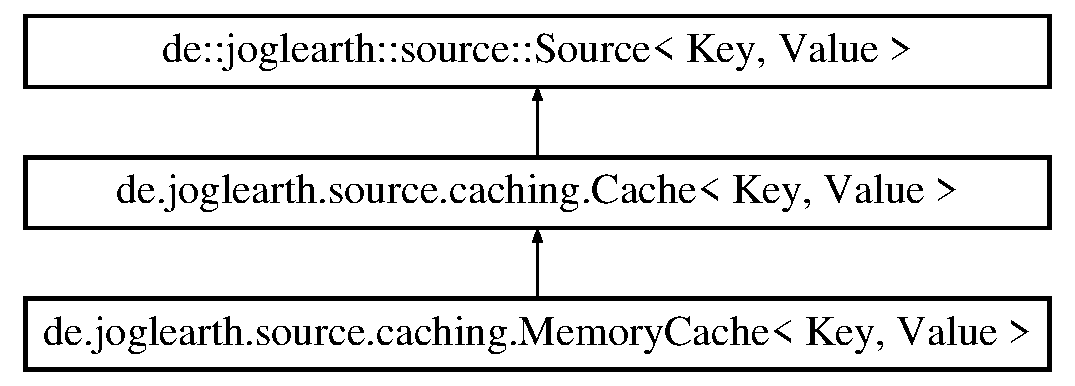
\includegraphics[height=2.000000cm]{classde_1_1joglearth_1_1source_1_1caching_1_1_memory_cache_3_01_key_00_01_value_01_4}
\end{center}
\end{figure}
\subsection*{Öffentliche Methoden}
\begin{DoxyCompactItemize}
\item 
Source\-Response$<$ Value $>$ {\bfseries request\-Object} (Key key, Source\-Listener$<$ Key, Value $>$ sender)\label{classde_1_1joglearth_1_1source_1_1caching_1_1_memory_cache_3_01_key_00_01_value_01_4_a29833385da6c6b96c56544425dc78d52}

\item 
void {\bf put\-Object} (Key key, Value value)
\item 
void {\bf drop\-Object} (Key key)
\item 
Iterable$<$ Key $>$ {\bf get\-Existing\-Objects} ()
\item 
void {\bf drop\-All} ()
\end{DoxyCompactItemize}


\subsection{Ausführliche Beschreibung}
Implements the \doxyref{Cache}{S.}{} interface in such way that it stores objects in the memory. 

\subsection{Dokumentation der Elementfunktionen}
\index{de\-::joglearth\-::source\-::caching\-::\-Memory\-Cache$<$ Key, Value $>$@{de\-::joglearth\-::source\-::caching\-::\-Memory\-Cache$<$ Key, Value $>$}!drop\-All@{drop\-All}}
\index{drop\-All@{drop\-All}!de::joglearth::source::caching::MemoryCache< Key, Value >@{de\-::joglearth\-::source\-::caching\-::\-Memory\-Cache$<$ Key, Value $>$}}
\subsubsection[{drop\-All}]{\setlength{\rightskip}{0pt plus 5cm}void de.\-joglearth.\-source.\-caching.\-Memory\-Cache$<$ Key, Value $>$.drop\-All (
\begin{DoxyParamCaption}
{}
\end{DoxyParamCaption}
)}\label{classde_1_1joglearth_1_1source_1_1caching_1_1_memory_cache_3_01_key_00_01_value_01_4_a704e4bb8f34123141f5175f4a22386d0}
Drops all objects contained in a cache. 

Implementiert {\bf de.\-joglearth.\-source.\-caching.\-Cache$<$ Key, Value $>$} \doxyref{}{S.}{interfacede_1_1joglearth_1_1source_1_1caching_1_1_cache_3_01_key_00_01_value_01_4_a5f80139900d2147330955a4bfd865581}.

\index{de\-::joglearth\-::source\-::caching\-::\-Memory\-Cache$<$ Key, Value $>$@{de\-::joglearth\-::source\-::caching\-::\-Memory\-Cache$<$ Key, Value $>$}!drop\-Object@{drop\-Object}}
\index{drop\-Object@{drop\-Object}!de::joglearth::source::caching::MemoryCache< Key, Value >@{de\-::joglearth\-::source\-::caching\-::\-Memory\-Cache$<$ Key, Value $>$}}
\subsubsection[{drop\-Object}]{\setlength{\rightskip}{0pt plus 5cm}void de.\-joglearth.\-source.\-caching.\-Memory\-Cache$<$ Key, Value $>$.drop\-Object (
\begin{DoxyParamCaption}
\item[{Key}]{k}
\end{DoxyParamCaption}
)}\label{classde_1_1joglearth_1_1source_1_1caching_1_1_memory_cache_3_01_key_00_01_value_01_4_a33c591b306da4105b8703321c5765618}
Erases the reference to an object if the {\ttfamily Key} is a valid I\-D of a stored object.


\begin{DoxyParams}{Parameter}
{\em k} & The I\-D of object to be dropped \\
\hline
\end{DoxyParams}


Implementiert {\bf de.\-joglearth.\-source.\-caching.\-Cache$<$ Key, Value $>$} \doxyref{}{S.}{interfacede_1_1joglearth_1_1source_1_1caching_1_1_cache_3_01_key_00_01_value_01_4_a8489bd44c6848442a8aa8cc7c4a13cb0}.

\index{de\-::joglearth\-::source\-::caching\-::\-Memory\-Cache$<$ Key, Value $>$@{de\-::joglearth\-::source\-::caching\-::\-Memory\-Cache$<$ Key, Value $>$}!get\-Existing\-Objects@{get\-Existing\-Objects}}
\index{get\-Existing\-Objects@{get\-Existing\-Objects}!de::joglearth::source::caching::MemoryCache< Key, Value >@{de\-::joglearth\-::source\-::caching\-::\-Memory\-Cache$<$ Key, Value $>$}}
\subsubsection[{get\-Existing\-Objects}]{\setlength{\rightskip}{0pt plus 5cm}Iterable$<$Key$>$ de.\-joglearth.\-source.\-caching.\-Memory\-Cache$<$ Key, Value $>$.get\-Existing\-Objects (
\begin{DoxyParamCaption}
{}
\end{DoxyParamCaption}
)}\label{classde_1_1joglearth_1_1source_1_1caching_1_1_memory_cache_3_01_key_00_01_value_01_4_a98e5a449b0ced05c622c782a8aa1f1ec}
Can be used to get the objects that already exist when the cache is initialized. \begin{DoxyReturn}{Rückgabe}
All stored objects 
\end{DoxyReturn}


Implementiert {\bf de.\-joglearth.\-source.\-caching.\-Cache$<$ Key, Value $>$} \doxyref{}{S.}{interfacede_1_1joglearth_1_1source_1_1caching_1_1_cache_3_01_key_00_01_value_01_4_a482408fd3c7be507f7d51b421889a725}.

\index{de\-::joglearth\-::source\-::caching\-::\-Memory\-Cache$<$ Key, Value $>$@{de\-::joglearth\-::source\-::caching\-::\-Memory\-Cache$<$ Key, Value $>$}!put\-Object@{put\-Object}}
\index{put\-Object@{put\-Object}!de::joglearth::source::caching::MemoryCache< Key, Value >@{de\-::joglearth\-::source\-::caching\-::\-Memory\-Cache$<$ Key, Value $>$}}
\subsubsection[{put\-Object}]{\setlength{\rightskip}{0pt plus 5cm}void de.\-joglearth.\-source.\-caching.\-Memory\-Cache$<$ Key, Value $>$.put\-Object (
\begin{DoxyParamCaption}
\item[{Key}]{k, }
\item[{Value}]{v}
\end{DoxyParamCaption}
)}\label{classde_1_1joglearth_1_1source_1_1caching_1_1_memory_cache_3_01_key_00_01_value_01_4_a1c757dc21fa73d5318867db45002aae2}
Stores object identified by a {\ttfamily Key}. An existing object with that {\ttfamily Key} may be overwritten.


\begin{DoxyParams}{Parameter}
{\em k} & I\-D of object \\
\hline
{\em v} & The object to be stored \\
\hline
\end{DoxyParams}


Implementiert {\bf de.\-joglearth.\-source.\-caching.\-Cache$<$ Key, Value $>$} \doxyref{}{S.}{interfacede_1_1joglearth_1_1source_1_1caching_1_1_cache_3_01_key_00_01_value_01_4_ad2c805820ba476907fd53b4dcb255d50}.


\section{de.\-joglearth.\-rendering.\-Mesh Klassenreferenz}
\label{classde_1_1joglearth_1_1rendering_1_1_mesh}\index{de.\-joglearth.\-rendering.\-Mesh@{de.\-joglearth.\-rendering.\-Mesh}}
\subsection*{Öffentliche Methoden}
\begin{DoxyCompactItemize}
\item 
{\bf Mesh} (float[$\,$] {\bf vertices}, int {\bf gl\-Vertex\-Format}, int[$\,$] {\bf indices})
\item 
{\bf Mesh} ()
\end{DoxyCompactItemize}
\subsection*{Öffentliche Attribute}
\begin{DoxyCompactItemize}
\item 
float[$\,$] {\bf vertices} = null
\item 
int {\bf gl\-Vertex\-Format} = G\-L2.\-G\-L\-\_\-\-T2\-F\-\_\-\-N3\-F\-\_\-\-V3\-F
\item 
int[$\,$] {\bf indices} = null
\end{DoxyCompactItemize}


\subsection{Ausführliche Beschreibung}
Container class to save vertices, normals and texture coordinates and other parameters to build a tile. 

\subsection{Beschreibung der Konstruktoren und Destruktoren}
\index{de\-::joglearth\-::rendering\-::\-Mesh@{de\-::joglearth\-::rendering\-::\-Mesh}!Mesh@{Mesh}}
\index{Mesh@{Mesh}!de::joglearth::rendering::Mesh@{de\-::joglearth\-::rendering\-::\-Mesh}}
\subsubsection[{Mesh}]{\setlength{\rightskip}{0pt plus 5cm}de.\-joglearth.\-rendering.\-Mesh.\-Mesh (
\begin{DoxyParamCaption}
\item[{float[$\,$]}]{vertices, }
\item[{int}]{gl\-Vertex\-Format, }
\item[{int[$\,$]}]{indices}
\end{DoxyParamCaption}
)}\label{classde_1_1joglearth_1_1rendering_1_1_mesh_ad96a6527669ee20829cfcb14998af60d}
Constructor. Initializes the \doxyref{Mesh}{S.}{classde_1_1joglearth_1_1rendering_1_1_mesh}


\begin{DoxyParams}{Parameter}
{\em vertices} & The array of vertices, normals and texture coordinates according to the vertex format. \\
\hline
{\em gl\-Vertex\-Format} & The Open\-G\-L vertex format used. Describes the layout of the vertex array. \\
\hline
{\em indices} & The array of indices. \\
\hline
\end{DoxyParams}
\index{de\-::joglearth\-::rendering\-::\-Mesh@{de\-::joglearth\-::rendering\-::\-Mesh}!Mesh@{Mesh}}
\index{Mesh@{Mesh}!de::joglearth::rendering::Mesh@{de\-::joglearth\-::rendering\-::\-Mesh}}
\subsubsection[{Mesh}]{\setlength{\rightskip}{0pt plus 5cm}de.\-joglearth.\-rendering.\-Mesh.\-Mesh (
\begin{DoxyParamCaption}
{}
\end{DoxyParamCaption}
)}\label{classde_1_1joglearth_1_1rendering_1_1_mesh_a2497af1e7a6a39fc0d7ca63e24a5bed7}
Default constructor. Initializes an empty \doxyref{Mesh}{S.}{classde_1_1joglearth_1_1rendering_1_1_mesh}. 

\subsection{Dokumentation der Datenelemente}
\index{de\-::joglearth\-::rendering\-::\-Mesh@{de\-::joglearth\-::rendering\-::\-Mesh}!gl\-Vertex\-Format@{gl\-Vertex\-Format}}
\index{gl\-Vertex\-Format@{gl\-Vertex\-Format}!de::joglearth::rendering::Mesh@{de\-::joglearth\-::rendering\-::\-Mesh}}
\subsubsection[{gl\-Vertex\-Format}]{\setlength{\rightskip}{0pt plus 5cm}int de.\-joglearth.\-rendering.\-Mesh.\-gl\-Vertex\-Format = G\-L2.\-G\-L\-\_\-\-T2\-F\-\_\-\-N3\-F\-\_\-\-V3\-F}\label{classde_1_1joglearth_1_1rendering_1_1_mesh_a355e6a00994dc073710ace1cb59b67ae}
The vertex format, as specified by Open\-G\-L. \index{de\-::joglearth\-::rendering\-::\-Mesh@{de\-::joglearth\-::rendering\-::\-Mesh}!indices@{indices}}
\index{indices@{indices}!de::joglearth::rendering::Mesh@{de\-::joglearth\-::rendering\-::\-Mesh}}
\subsubsection[{indices}]{\setlength{\rightskip}{0pt plus 5cm}int [$\,$] de.\-joglearth.\-rendering.\-Mesh.\-indices = null}\label{classde_1_1joglearth_1_1rendering_1_1_mesh_a7aa6d61511c82f451c9b75b8b7bf1cf6}
The array of indices used to iterate over the vertex array. \index{de\-::joglearth\-::rendering\-::\-Mesh@{de\-::joglearth\-::rendering\-::\-Mesh}!vertices@{vertices}}
\index{vertices@{vertices}!de::joglearth::rendering::Mesh@{de\-::joglearth\-::rendering\-::\-Mesh}}
\subsubsection[{vertices}]{\setlength{\rightskip}{0pt plus 5cm}float [$\,$] de.\-joglearth.\-rendering.\-Mesh.\-vertices = null}\label{classde_1_1joglearth_1_1rendering_1_1_mesh_a78c0fca31a542fc6d7261bdd9428643a}
The array of vertices. Elements are treated as dictated by the {\ttfamily gl\-Vertex\-Format}. 
\section{de.\-joglearth.\-ui.\-Named\-Item$<$ E $>$ Klassenreferenz}
\label{classde_1_1joglearth_1_1ui_1_1_named_item_3_01_e_01_4}\index{de.\-joglearth.\-ui.\-Named\-Item$<$ E $>$@{de.\-joglearth.\-ui.\-Named\-Item$<$ E $>$}}
Klassendiagramm für de.\-joglearth.\-ui.\-Named\-Item$<$ E $>$\-:\begin{figure}[H]
\begin{center}
\leavevmode
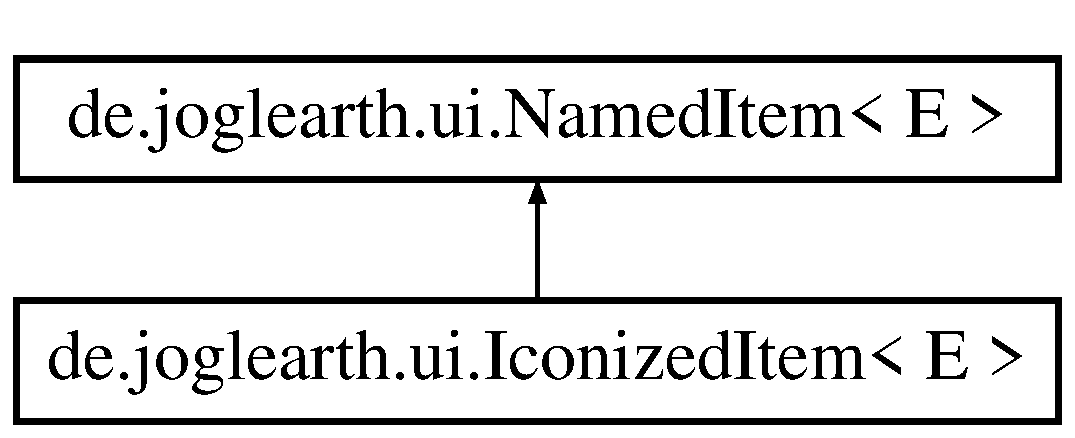
\includegraphics[height=2.000000cm]{classde_1_1joglearth_1_1ui_1_1_named_item_3_01_e_01_4}
\end{center}
\end{figure}
\subsection*{Öffentliche Methoden}
\begin{DoxyCompactItemize}
\item 
{\bf Named\-Item} (String caption, E value)
\item 
String {\bf to\-String} ()
\item 
E {\bf get\-Value} ()
\end{DoxyCompactItemize}


\subsection{Ausführliche Beschreibung}
Aggregation of a string caption and a generic value used to map values to captions inside Combo\-Boxes or Lists.


\begin{DoxyParams}{Parameter}
{\em E} & The generic type. \\
\hline
\end{DoxyParams}


\subsection{Beschreibung der Konstruktoren und Destruktoren}
\index{de\-::joglearth\-::ui\-::\-Named\-Item$<$ E $>$@{de\-::joglearth\-::ui\-::\-Named\-Item$<$ E $>$}!Named\-Item@{Named\-Item}}
\index{Named\-Item@{Named\-Item}!de::joglearth::ui::NamedItem< E >@{de\-::joglearth\-::ui\-::\-Named\-Item$<$ E $>$}}
\subsubsection[{Named\-Item}]{\setlength{\rightskip}{0pt plus 5cm}de.\-joglearth.\-ui.\-Named\-Item$<$ E $>$.Named\-Item (
\begin{DoxyParamCaption}
\item[{String}]{caption, }
\item[{E}]{value}
\end{DoxyParamCaption}
)}\label{classde_1_1joglearth_1_1ui_1_1_named_item_3_01_e_01_4_a7a4c9c32286b665eeadbac079cb43390}
Constructor.


\begin{DoxyParams}{Parameter}
{\em caption} & The caption, later returned by {\ttfamily \doxyref{to\-String()}{S.}{classde_1_1joglearth_1_1ui_1_1_named_item_3_01_e_01_4_aad33c70bdfe3d07be8df933a9ad7dc2f}} \\
\hline
{\em value} & The value to map to \\
\hline
\end{DoxyParams}


\subsection{Dokumentation der Elementfunktionen}
\index{de\-::joglearth\-::ui\-::\-Named\-Item$<$ E $>$@{de\-::joglearth\-::ui\-::\-Named\-Item$<$ E $>$}!get\-Value@{get\-Value}}
\index{get\-Value@{get\-Value}!de::joglearth::ui::NamedItem< E >@{de\-::joglearth\-::ui\-::\-Named\-Item$<$ E $>$}}
\subsubsection[{get\-Value}]{\setlength{\rightskip}{0pt plus 5cm}E de.\-joglearth.\-ui.\-Named\-Item$<$ E $>$.get\-Value (
\begin{DoxyParamCaption}
{}
\end{DoxyParamCaption}
)}\label{classde_1_1joglearth_1_1ui_1_1_named_item_3_01_e_01_4_a2303af63ccfccf5617c5cbc5658ca36d}
Returns the item's svalue. \index{de\-::joglearth\-::ui\-::\-Named\-Item$<$ E $>$@{de\-::joglearth\-::ui\-::\-Named\-Item$<$ E $>$}!to\-String@{to\-String}}
\index{to\-String@{to\-String}!de::joglearth::ui::NamedItem< E >@{de\-::joglearth\-::ui\-::\-Named\-Item$<$ E $>$}}
\subsubsection[{to\-String}]{\setlength{\rightskip}{0pt plus 5cm}String de.\-joglearth.\-ui.\-Named\-Item$<$ E $>$.to\-String (
\begin{DoxyParamCaption}
{}
\end{DoxyParamCaption}
)}\label{classde_1_1joglearth_1_1ui_1_1_named_item_3_01_e_01_4_aad33c70bdfe3d07be8df933a9ad7dc2f}
Returns the caption. 
\section{de.\-joglearth.\-source.\-nominatim.\-Nominatim\-Manager Klassenreferenz}
\label{classde_1_1joglearth_1_1source_1_1nominatim_1_1_nominatim_manager}\index{de.\-joglearth.\-source.\-nominatim.\-Nominatim\-Manager@{de.\-joglearth.\-source.\-nominatim.\-Nominatim\-Manager}}


Abgeleitet von Source$<$ Nominatim\-Query, Collection$<$ Location $>$ $>$.

\subsection*{Öffentliche Methoden}
\begin{DoxyCompactItemize}
\item 
Source\-Response$<$ Collection\\*
$<$ {\bf Location} $>$ $>$ {\bfseries request\-Object} ({\bf Nominatim\-Query} key, Source\-Listener$<$ {\bf Nominatim\-Query}, Collection$<$ {\bf Location} $>$$>$ sender)\label{classde_1_1joglearth_1_1source_1_1nominatim_1_1_nominatim_manager_ae292fe5eeddb395ffda6a6922d759733}

\item 
void {\bf set\-Cache\-Size} (int cache\-Size)
\end{DoxyCompactItemize}
\subsection*{Öffentliche, statische Methoden}
\begin{DoxyCompactItemize}
\item 
static {\bf Nominatim\-Manager} {\bf get\-Instance} ()
\end{DoxyCompactItemize}


\subsection{Ausführliche Beschreibung}
Singleton class that retrieves data from the \doxyref{Nominatim\-Source}{S.}{classde_1_1joglearth_1_1source_1_1nominatim_1_1_nominatim_source}. 

\subsection{Dokumentation der Elementfunktionen}
\index{de\-::joglearth\-::source\-::nominatim\-::\-Nominatim\-Manager@{de\-::joglearth\-::source\-::nominatim\-::\-Nominatim\-Manager}!get\-Instance@{get\-Instance}}
\index{get\-Instance@{get\-Instance}!de::joglearth::source::nominatim::NominatimManager@{de\-::joglearth\-::source\-::nominatim\-::\-Nominatim\-Manager}}
\subsubsection[{get\-Instance}]{\setlength{\rightskip}{0pt plus 5cm}static {\bf Nominatim\-Manager} de.\-joglearth.\-source.\-nominatim.\-Nominatim\-Manager.\-get\-Instance (
\begin{DoxyParamCaption}
{}
\end{DoxyParamCaption}
)\hspace{0.3cm}{\ttfamily [static]}}\label{classde_1_1joglearth_1_1source_1_1nominatim_1_1_nominatim_manager_aaa7bdec62233b4724949821bd1f4add8}
Returns the instance of the class or creates it, if it does not exist yet.

\begin{DoxyReturn}{Rückgabe}
The instance of {\ttfamily \doxyref{Nominatim\-Manager}{S.}{classde_1_1joglearth_1_1source_1_1nominatim_1_1_nominatim_manager}} 
\end{DoxyReturn}
\index{de\-::joglearth\-::source\-::nominatim\-::\-Nominatim\-Manager@{de\-::joglearth\-::source\-::nominatim\-::\-Nominatim\-Manager}!set\-Cache\-Size@{set\-Cache\-Size}}
\index{set\-Cache\-Size@{set\-Cache\-Size}!de::joglearth::source::nominatim::NominatimManager@{de\-::joglearth\-::source\-::nominatim\-::\-Nominatim\-Manager}}
\subsubsection[{set\-Cache\-Size}]{\setlength{\rightskip}{0pt plus 5cm}void de.\-joglearth.\-source.\-nominatim.\-Nominatim\-Manager.\-set\-Cache\-Size (
\begin{DoxyParamCaption}
\item[{int}]{cache\-Size}
\end{DoxyParamCaption}
)}\label{classde_1_1joglearth_1_1source_1_1nominatim_1_1_nominatim_manager_ae2a43b7a49f6d0cf9040380396f91169}
Sets the size of a \doxyref{Cache}{S.}{}. 
\begin{DoxyParams}{Parameter}
{\em cache\-Size} & The new size of the {\ttfamily Cache} \\
\hline
\end{DoxyParams}

\section{de.\-joglearth.\-source.\-nominatim.\-Nominatim\-Query Klassenreferenz}
\label{classde_1_1joglearth_1_1source_1_1nominatim_1_1_nominatim_query}\index{de.\-joglearth.\-source.\-nominatim.\-Nominatim\-Query@{de.\-joglearth.\-source.\-nominatim.\-Nominatim\-Query}}
\subsection*{Klassen}
\begin{DoxyCompactItemize}
\item 
enum {\bf Type}
\end{DoxyCompactItemize}
\subsection*{Öffentliche Methoden}
\begin{DoxyCompactItemize}
\item 
{\bf Nominatim\-Query} ({\bf Type} type)
\end{DoxyCompactItemize}
\subsection*{Öffentliche Attribute}
\begin{DoxyCompactItemize}
\item 
{\bf Type} {\bfseries type}\label{classde_1_1joglearth_1_1source_1_1nominatim_1_1_nominatim_query_a2ab5853d020ddc79a7e449ca244d0a0a}

\item 
{\bf Tile} {\bfseries area}\label{classde_1_1joglearth_1_1source_1_1nominatim_1_1_nominatim_query_a3c119db248acd431d576569f03ff52de}

\item 
{\bf Screen\-Coordinates} {\bfseries point}\label{classde_1_1joglearth_1_1source_1_1nominatim_1_1_nominatim_query_acd9afaaed849fd0eb140183f9fa63d9d}

\item 
String {\bfseries query}\label{classde_1_1joglearth_1_1source_1_1nominatim_1_1_nominatim_query_a445192f97ae082bfbf076d4231e75755}

\end{DoxyCompactItemize}


\subsection{Ausführliche Beschreibung}
Supports a query to Nominatim. There are three types of queries\-: G\-L\-O\-B\-A\-L, L\-O\-C\-A\-L, P\-O\-I\-N\-T. 

\subsection{Beschreibung der Konstruktoren und Destruktoren}
\index{de\-::joglearth\-::source\-::nominatim\-::\-Nominatim\-Query@{de\-::joglearth\-::source\-::nominatim\-::\-Nominatim\-Query}!Nominatim\-Query@{Nominatim\-Query}}
\index{Nominatim\-Query@{Nominatim\-Query}!de::joglearth::source::nominatim::NominatimQuery@{de\-::joglearth\-::source\-::nominatim\-::\-Nominatim\-Query}}
\subsubsection[{Nominatim\-Query}]{\setlength{\rightskip}{0pt plus 5cm}de.\-joglearth.\-source.\-nominatim.\-Nominatim\-Query.\-Nominatim\-Query (
\begin{DoxyParamCaption}
\item[{{\bf Type}}]{type}
\end{DoxyParamCaption}
)}\label{classde_1_1joglearth_1_1source_1_1nominatim_1_1_nominatim_query_a7c61c89b5c7c2416a52eb0222cac0978}
Constructor. Assigns a value to a \doxyref{Type}{S.}{enumde_1_1joglearth_1_1source_1_1nominatim_1_1_nominatim_query_1_1_type}.


\begin{DoxyParams}{Parameter}
{\em type} & The {\ttfamily \doxyref{Type}{S.}{enumde_1_1joglearth_1_1source_1_1nominatim_1_1_nominatim_query_1_1_type}} of the query \\
\hline
\end{DoxyParams}

\section{de.\-joglearth.\-source.\-nominatim.\-Nominatim\-Source Klassenreferenz}
\label{classde_1_1joglearth_1_1source_1_1nominatim_1_1_nominatim_source}\index{de.\-joglearth.\-source.\-nominatim.\-Nominatim\-Source@{de.\-joglearth.\-source.\-nominatim.\-Nominatim\-Source}}


Abgeleitet von Source$<$ Nominatim\-Query, Location[$\,$]$>$.

\subsection*{Öffentliche Methoden}
\begin{DoxyCompactItemize}
\item 
{\bf Nominatim\-Source} ()
\item 
Source\-Response$<$ {\bf Location}[$\,$]$>$ {\bfseries request\-Object} ({\bf Nominatim\-Query} key, Source\-Listener$<$ {\bf Nominatim\-Query}, {\bf Location}[$\,$]$>$ sender)\label{classde_1_1joglearth_1_1source_1_1nominatim_1_1_nominatim_source_aaf769f044078b055bbe251220e2a89e5}

\end{DoxyCompactItemize}


\subsection{Ausführliche Beschreibung}
Provides responses of search requests, for e.\-g. search requests for places or detailed information to a point. The response will be prepared for the \doxyref{Location\-Manager}{S.}{}; uses the \doxyref{H\-T\-T\-P}{S.}{} for the search request. 

\subsection{Beschreibung der Konstruktoren und Destruktoren}
\index{de\-::joglearth\-::source\-::nominatim\-::\-Nominatim\-Source@{de\-::joglearth\-::source\-::nominatim\-::\-Nominatim\-Source}!Nominatim\-Source@{Nominatim\-Source}}
\index{Nominatim\-Source@{Nominatim\-Source}!de::joglearth::source::nominatim::NominatimSource@{de\-::joglearth\-::source\-::nominatim\-::\-Nominatim\-Source}}
\subsubsection[{Nominatim\-Source}]{\setlength{\rightskip}{0pt plus 5cm}de.\-joglearth.\-source.\-nominatim.\-Nominatim\-Source.\-Nominatim\-Source (
\begin{DoxyParamCaption}
{}
\end{DoxyParamCaption}
)}\label{classde_1_1joglearth_1_1source_1_1nominatim_1_1_nominatim_source_ad34f141b072b420a7849228a3b9287d5}
Constructor. Initializes the \doxyref{Nominatim\-Source}{S.}{classde_1_1joglearth_1_1source_1_1nominatim_1_1_nominatim_source}. 
\section{de.\-joglearth.\-source.\-caching.\-Object\-Measure$<$ T $>$ Schnittstellenreferenz}
\label{interfacede_1_1joglearth_1_1source_1_1caching_1_1_object_measure_3_01_t_01_4}\index{de.\-joglearth.\-source.\-caching.\-Object\-Measure$<$ T $>$@{de.\-joglearth.\-source.\-caching.\-Object\-Measure$<$ T $>$}}
Klassendiagramm für de.\-joglearth.\-source.\-caching.\-Object\-Measure$<$ T $>$\-:\begin{figure}[H]
\begin{center}
\leavevmode
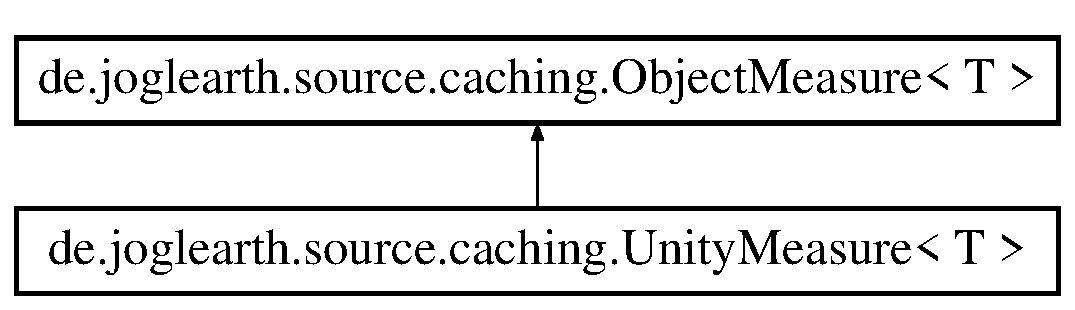
\includegraphics[height=2.000000cm]{interfacede_1_1joglearth_1_1source_1_1caching_1_1_object_measure_3_01_t_01_4}
\end{center}
\end{figure}
\subsection*{Öffentliche Methoden}
\begin{DoxyCompactItemize}
\item 
int {\bf get\-Size} (T object)
\end{DoxyCompactItemize}


\subsection{Ausführliche Beschreibung}
Interface for classes assigning sizes to objects. 
\begin{DoxyParams}{Parameter}
{\em $<$\-T$>$} & The type to measure \\
\hline
\end{DoxyParams}


\subsection{Dokumentation der Elementfunktionen}
\index{de\-::joglearth\-::source\-::caching\-::\-Object\-Measure$<$ T $>$@{de\-::joglearth\-::source\-::caching\-::\-Object\-Measure$<$ T $>$}!get\-Size@{get\-Size}}
\index{get\-Size@{get\-Size}!de::joglearth::source::caching::ObjectMeasure< T >@{de\-::joglearth\-::source\-::caching\-::\-Object\-Measure$<$ T $>$}}
\subsubsection[{get\-Size}]{\setlength{\rightskip}{0pt plus 5cm}int de.\-joglearth.\-source.\-caching.\-Object\-Measure$<$ T $>$.get\-Size (
\begin{DoxyParamCaption}
\item[{T}]{object}
\end{DoxyParamCaption}
)}\label{interfacede_1_1joglearth_1_1source_1_1caching_1_1_object_measure_3_01_t_01_4_a1d7e082d696fb43f94fbade17deb9f2c}
Determines the size of an object in a unit specific to the implementing class. 
\begin{DoxyParams}{Parameter}
{\em object} & The object to measure \\
\hline
\end{DoxyParams}
\begin{DoxyReturn}{Rückgabe}
The size, in units. Must be greater or equal 1 
\end{DoxyReturn}


Implementiert in {\bf de.\-joglearth.\-source.\-caching.\-Unity\-Measure$<$ T $>$} \doxyref{}{S.}{classde_1_1joglearth_1_1source_1_1caching_1_1_unity_measure_3_01_t_01_4_a2fe8769ef6b5b550d83169ef02eebb90}.


\section{de.\-joglearth.\-source.\-osm.\-O\-S\-M\-Path\-Translator Klassenreferenz}
\label{classde_1_1joglearth_1_1source_1_1osm_1_1_o_s_m_path_translator}\index{de.\-joglearth.\-source.\-osm.\-O\-S\-M\-Path\-Translator@{de.\-joglearth.\-source.\-osm.\-O\-S\-M\-Path\-Translator}}
Klassendiagramm für de.\-joglearth.\-source.\-osm.\-O\-S\-M\-Path\-Translator\-:\begin{figure}[H]
\begin{center}
\leavevmode
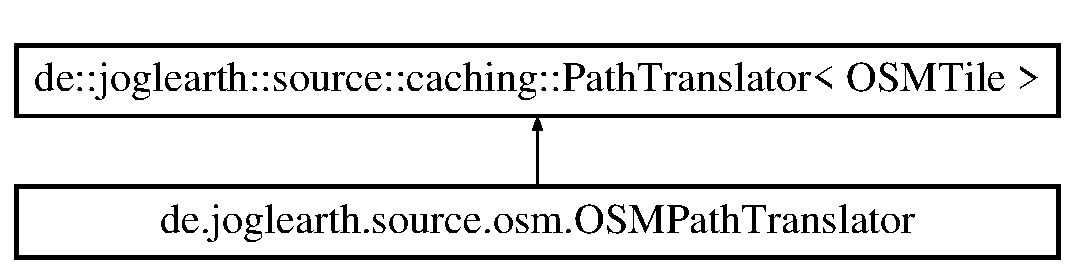
\includegraphics[height=2.000000cm]{classde_1_1joglearth_1_1source_1_1osm_1_1_o_s_m_path_translator}
\end{center}
\end{figure}
\subsection*{Öffentliche Methoden}
\begin{DoxyCompactItemize}
\item 
String {\bfseries to\-File\-System\-Path} ({\bf O\-S\-M\-Tile} k)\label{classde_1_1joglearth_1_1source_1_1osm_1_1_o_s_m_path_translator_a2bd303d6f40581fd5409047569441725}

\item 
{\bf O\-S\-M\-Tile} {\bfseries from\-File\-System\-Path} (String s)\label{classde_1_1joglearth_1_1source_1_1osm_1_1_o_s_m_path_translator_a9b1c06866ae1e7c1def9a535d0dda798}

\end{DoxyCompactItemize}


\subsection{Ausführliche Beschreibung}
Implements the \doxyref{Path\-Translator}{S.}{} interface \doxyref{O\-S\-M\-Tile}{S.}{classde_1_1joglearth_1_1source_1_1osm_1_1_o_s_m_tile}s. 
\section{de.\-joglearth.\-source.\-osm.\-O\-S\-M\-Tile Klassenreferenz}
\label{classde_1_1joglearth_1_1source_1_1osm_1_1_o_s_m_tile}\index{de.\-joglearth.\-source.\-osm.\-O\-S\-M\-Tile@{de.\-joglearth.\-source.\-osm.\-O\-S\-M\-Tile}}
\subsection*{Öffentliche Attribute}
\begin{DoxyCompactItemize}
\item 
{\bf Tile} {\bfseries tile}\label{classde_1_1joglearth_1_1source_1_1osm_1_1_o_s_m_tile_a1397a0f96b9d8f5e60c3a5edab46b2f3}

\item 
{\bf Tiled\-Map\-Type} {\bfseries type}\label{classde_1_1joglearth_1_1source_1_1osm_1_1_o_s_m_tile_a90c20737534ceb4ccc2438d6fe3d96dd}

\end{DoxyCompactItemize}

\section{de.\-joglearth.\-source.\-osm.\-O\-S\-M\-Tile\-Manager Klassenreferenz}
\label{classde_1_1joglearth_1_1source_1_1osm_1_1_o_s_m_tile_manager}\index{de.\-joglearth.\-source.\-osm.\-O\-S\-M\-Tile\-Manager@{de.\-joglearth.\-source.\-osm.\-O\-S\-M\-Tile\-Manager}}
Klassendiagramm für de.\-joglearth.\-source.\-osm.\-O\-S\-M\-Tile\-Manager\-:\begin{figure}[H]
\begin{center}
\leavevmode
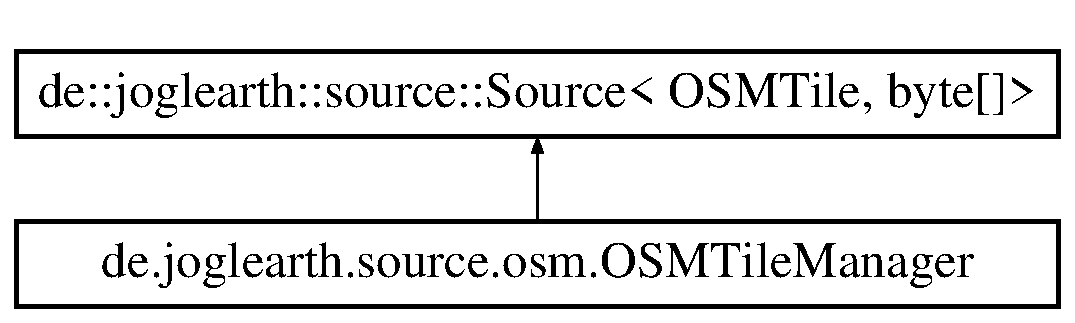
\includegraphics[height=2.000000cm]{classde_1_1joglearth_1_1source_1_1osm_1_1_o_s_m_tile_manager}
\end{center}
\end{figure}
\subsection*{Öffentliche Methoden}
\begin{DoxyCompactItemize}
\item 
Source\-Response$<$ byte[$\,$]$>$ {\bfseries request\-Object} ({\bf O\-S\-M\-Tile} key, Source\-Listener$<$ {\bf O\-S\-M\-Tile}, byte[$\,$]$>$ sender)\label{classde_1_1joglearth_1_1source_1_1osm_1_1_o_s_m_tile_manager_acb86a61ab9d3572ed510b45bada76a26}

\item 
void {\bf set\-Cache\-Size} (int cache\-Size)
\end{DoxyCompactItemize}
\subsection*{Öffentliche, statische Methoden}
\begin{DoxyCompactItemize}
\item 
static {\bf O\-S\-M\-Tile\-Manager} {\bf get\-Instance} ()
\end{DoxyCompactItemize}


\subsection{Ausführliche Beschreibung}
Singleton class that retrieves data from the \doxyref{O\-S\-M\-Tile\-Source}{S.}{classde_1_1joglearth_1_1source_1_1osm_1_1_o_s_m_tile_source}. 

\subsection{Dokumentation der Elementfunktionen}
\index{de\-::joglearth\-::source\-::osm\-::\-O\-S\-M\-Tile\-Manager@{de\-::joglearth\-::source\-::osm\-::\-O\-S\-M\-Tile\-Manager}!get\-Instance@{get\-Instance}}
\index{get\-Instance@{get\-Instance}!de::joglearth::source::osm::OSMTileManager@{de\-::joglearth\-::source\-::osm\-::\-O\-S\-M\-Tile\-Manager}}
\subsubsection[{get\-Instance}]{\setlength{\rightskip}{0pt plus 5cm}static {\bf O\-S\-M\-Tile\-Manager} de.\-joglearth.\-source.\-osm.\-O\-S\-M\-Tile\-Manager.\-get\-Instance (
\begin{DoxyParamCaption}
{}
\end{DoxyParamCaption}
)\hspace{0.3cm}{\ttfamily [static]}}\label{classde_1_1joglearth_1_1source_1_1osm_1_1_o_s_m_tile_manager_a132bf30ed8003964deda8bb2214acc27}
Returns the instance of the class or creates it, if it does not exist yet.

\begin{DoxyReturn}{Rückgabe}
The instance of \doxyref{O\-S\-M\-Tile\-Manager}{S.}{classde_1_1joglearth_1_1source_1_1osm_1_1_o_s_m_tile_manager} 
\end{DoxyReturn}
\index{de\-::joglearth\-::source\-::osm\-::\-O\-S\-M\-Tile\-Manager@{de\-::joglearth\-::source\-::osm\-::\-O\-S\-M\-Tile\-Manager}!set\-Cache\-Size@{set\-Cache\-Size}}
\index{set\-Cache\-Size@{set\-Cache\-Size}!de::joglearth::source::osm::OSMTileManager@{de\-::joglearth\-::source\-::osm\-::\-O\-S\-M\-Tile\-Manager}}
\subsubsection[{set\-Cache\-Size}]{\setlength{\rightskip}{0pt plus 5cm}void de.\-joglearth.\-source.\-osm.\-O\-S\-M\-Tile\-Manager.\-set\-Cache\-Size (
\begin{DoxyParamCaption}
\item[{int}]{cache\-Size}
\end{DoxyParamCaption}
)}\label{classde_1_1joglearth_1_1source_1_1osm_1_1_o_s_m_tile_manager_aae8e7bab613b9504c1de76626ac87f8b}
Sets the size of a \doxyref{Cache}{S.}{}. 
\begin{DoxyParams}{Parameter}
{\em cache\-Size} & the new size of the {\ttfamily Cache} \\
\hline
\end{DoxyParams}

\section{de.\-joglearth.\-source.\-osm.\-O\-S\-M\-Tile\-Source Klassenreferenz}
\label{classde_1_1joglearth_1_1source_1_1osm_1_1_o_s_m_tile_source}\index{de.\-joglearth.\-source.\-osm.\-O\-S\-M\-Tile\-Source@{de.\-joglearth.\-source.\-osm.\-O\-S\-M\-Tile\-Source}}


Abgeleitet von Source$<$ O\-S\-M\-Tile, byte[$\,$]$>$.

\subsection*{Öffentliche Methoden}
\begin{DoxyCompactItemize}
\item 
{\bf O\-S\-M\-Tile\-Source} (String[$\,$] servers)
\item 
Source\-Response$<$ byte[$\,$]$>$ {\bfseries request\-Object} ({\bf O\-S\-M\-Tile} k, Source\-Listener$<$ {\bf O\-S\-M\-Tile}, byte[$\,$]$>$ sender)\label{classde_1_1joglearth_1_1source_1_1osm_1_1_o_s_m_tile_source_ad557ab5983704a9adbdf065e4d0affe4}

\item 
void {\bf set\-Tile\-Type} ({\bf Tiled\-Map\-Type} type)
\end{DoxyCompactItemize}


\subsection{Ausführliche Beschreibung}
Loads Open\-Street\-Map image tiles by their coordinates via H\-T\-T\-P. 

\subsection{Beschreibung der Konstruktoren und Destruktoren}
\index{de\-::joglearth\-::source\-::osm\-::\-O\-S\-M\-Tile\-Source@{de\-::joglearth\-::source\-::osm\-::\-O\-S\-M\-Tile\-Source}!O\-S\-M\-Tile\-Source@{O\-S\-M\-Tile\-Source}}
\index{O\-S\-M\-Tile\-Source@{O\-S\-M\-Tile\-Source}!de::joglearth::source::osm::OSMTileSource@{de\-::joglearth\-::source\-::osm\-::\-O\-S\-M\-Tile\-Source}}
\subsubsection[{O\-S\-M\-Tile\-Source}]{\setlength{\rightskip}{0pt plus 5cm}de.\-joglearth.\-source.\-osm.\-O\-S\-M\-Tile\-Source.\-O\-S\-M\-Tile\-Source (
\begin{DoxyParamCaption}
\item[{String[$\,$]}]{servers}
\end{DoxyParamCaption}
)}\label{classde_1_1joglearth_1_1source_1_1osm_1_1_o_s_m_tile_source_a04bfa05850c44b43978c898666225b3e}
Constructor. Initializes the \doxyref{de.\-joglearth.\-source.\-osm.\-O\-S\-M\-Tile\-Source}{S.}{}.


\begin{DoxyParams}{Parameter}
{\em servers} & An array containing the server strings \\
\hline
\end{DoxyParams}


\subsection{Dokumentation der Elementfunktionen}
\index{de\-::joglearth\-::source\-::osm\-::\-O\-S\-M\-Tile\-Source@{de\-::joglearth\-::source\-::osm\-::\-O\-S\-M\-Tile\-Source}!set\-Tile\-Type@{set\-Tile\-Type}}
\index{set\-Tile\-Type@{set\-Tile\-Type}!de::joglearth::source::osm::OSMTileSource@{de\-::joglearth\-::source\-::osm\-::\-O\-S\-M\-Tile\-Source}}
\subsubsection[{set\-Tile\-Type}]{\setlength{\rightskip}{0pt plus 5cm}void de.\-joglearth.\-source.\-osm.\-O\-S\-M\-Tile\-Source.\-set\-Tile\-Type (
\begin{DoxyParamCaption}
\item[{{\bf Tiled\-Map\-Type}}]{type}
\end{DoxyParamCaption}
)}\label{classde_1_1joglearth_1_1source_1_1osm_1_1_o_s_m_tile_source_a8ed4fb9e841804d2b86e0aca3f477465}
Sets the type of an Open\-Street\-Map tile.


\begin{DoxyParams}{Parameter}
{\em type} & {\ttfamily Tiled\-Map\-Type} of the tile \\
\hline
\end{DoxyParams}

\section{de.\-joglearth.\-source.\-overpass.\-Overpass\-Manager Klassenreferenz}
\label{classde_1_1joglearth_1_1source_1_1overpass_1_1_overpass_manager}\index{de.\-joglearth.\-source.\-overpass.\-Overpass\-Manager@{de.\-joglearth.\-source.\-overpass.\-Overpass\-Manager}}


Abgeleitet von Source$<$ Overpass\-Query, Collection$<$ Location $>$ $>$.

\subsection*{Öffentliche Methoden}
\begin{DoxyCompactItemize}
\item 
Source\-Response$<$ Collection\\*
$<$ {\bf Location} $>$ $>$ {\bfseries request\-Object} ({\bf Overpass\-Query} key, Source\-Listener$<$ {\bf Overpass\-Query}, Collection$<$ {\bf Location} $>$$>$ sender)\label{classde_1_1joglearth_1_1source_1_1overpass_1_1_overpass_manager_af73881132282fbd32dc854999ed30e31}

\end{DoxyCompactItemize}
\subsection*{Öffentliche, statische Methoden}
\begin{DoxyCompactItemize}
\item 
static {\bf Overpass\-Manager} {\bf get\-Instance} ()
\end{DoxyCompactItemize}


\subsection{Ausführliche Beschreibung}
Singleton class that retrieves data from the \doxyref{de.\-joglearth.\-source.\-overpass.\-Overpass\-Source}{S.}{classde_1_1joglearth_1_1source_1_1overpass_1_1_overpass_source}. 

\subsection{Dokumentation der Elementfunktionen}
\index{de\-::joglearth\-::source\-::overpass\-::\-Overpass\-Manager@{de\-::joglearth\-::source\-::overpass\-::\-Overpass\-Manager}!get\-Instance@{get\-Instance}}
\index{get\-Instance@{get\-Instance}!de::joglearth::source::overpass::OverpassManager@{de\-::joglearth\-::source\-::overpass\-::\-Overpass\-Manager}}
\subsubsection[{get\-Instance}]{\setlength{\rightskip}{0pt plus 5cm}static {\bf Overpass\-Manager} de.\-joglearth.\-source.\-overpass.\-Overpass\-Manager.\-get\-Instance (
\begin{DoxyParamCaption}
{}
\end{DoxyParamCaption}
)\hspace{0.3cm}{\ttfamily [static]}}\label{classde_1_1joglearth_1_1source_1_1overpass_1_1_overpass_manager_aada32fad7d72548be2044392e313ef78}
Returns the instance of the class or creates it, if it does not exist yet.

\begin{DoxyReturn}{Rückgabe}
The instance of {\ttfamily \doxyref{Overpass\-Manager}{S.}{classde_1_1joglearth_1_1source_1_1overpass_1_1_overpass_manager}} 
\end{DoxyReturn}

\section{de.\-joglearth.\-source.\-overpass.\-Overpass\-Query Klassenreferenz}
\label{classde_1_1joglearth_1_1source_1_1overpass_1_1_overpass_query}\index{de.\-joglearth.\-source.\-overpass.\-Overpass\-Query@{de.\-joglearth.\-source.\-overpass.\-Overpass\-Query}}
\subsection*{Öffentliche Methoden}
\begin{DoxyCompactItemize}
\item 
{\bf Overpass\-Query} ({\bf Location\-Type} query, {\bf Tile} area)
\end{DoxyCompactItemize}
\subsection*{Öffentliche Attribute}
\begin{DoxyCompactItemize}
\item 
{\bf Tile} {\bfseries area}\label{classde_1_1joglearth_1_1source_1_1overpass_1_1_overpass_query_a39ee33605e2fbd63d4e8bb7fabd31046}

\item 
{\bf Location\-Type} {\bfseries query}\label{classde_1_1joglearth_1_1source_1_1overpass_1_1_overpass_query_a3d9b2ad642331614b222854b128b7dfa}

\end{DoxyCompactItemize}


\subsection{Ausführliche Beschreibung}
Supplies a query to the Overpass\-A\-P\-I. All results, e.\-g. P\-O\-Is or city names are within the F\-O\-V. The size of the F\-O\-V (the associated tiles) must be part of the query. 

\subsection{Beschreibung der Konstruktoren und Destruktoren}
\index{de\-::joglearth\-::source\-::overpass\-::\-Overpass\-Query@{de\-::joglearth\-::source\-::overpass\-::\-Overpass\-Query}!Overpass\-Query@{Overpass\-Query}}
\index{Overpass\-Query@{Overpass\-Query}!de::joglearth::source::overpass::OverpassQuery@{de\-::joglearth\-::source\-::overpass\-::\-Overpass\-Query}}
\subsubsection[{Overpass\-Query}]{\setlength{\rightskip}{0pt plus 5cm}de.\-joglearth.\-source.\-overpass.\-Overpass\-Query.\-Overpass\-Query (
\begin{DoxyParamCaption}
\item[{{\bf Location\-Type}}]{query, }
\item[{{\bf Tile}}]{area}
\end{DoxyParamCaption}
)}\label{classde_1_1joglearth_1_1source_1_1overpass_1_1_overpass_query_aaafab2ae81406a45092a78d8fa297a3b}
Constructor for a query in a given area. Assigns a value to a \doxyref{Location\-Type}{S.}{} and a \doxyref{Tile}{S.}{}.


\begin{DoxyParams}{Parameter}
{\em query} & The {\ttfamily Location\-Type} of the query \\
\hline
{\em area} & The {\ttfamily Tile} that determines where the query should be performed \\
\hline
\end{DoxyParams}

\section{de.\-joglearth.\-source.\-overpass.\-Overpass\-Source Klassenreferenz}
\label{classde_1_1joglearth_1_1source_1_1overpass_1_1_overpass_source}\index{de.\-joglearth.\-source.\-overpass.\-Overpass\-Source@{de.\-joglearth.\-source.\-overpass.\-Overpass\-Source}}


Abgeleitet von Source$<$ Overpass\-Query, Collection$<$ Location $>$ $>$.

\subsection*{Öffentliche Methoden}
\begin{DoxyCompactItemize}
\item 
Source\-Response$<$ Collection\\*
$<$ {\bf Location} $>$ $>$ {\bfseries request\-Object} ({\bf Overpass\-Query} key, Source\-Listener$<$ {\bf Overpass\-Query}, Collection$<$ {\bf Location} $>$$>$ sender)\label{classde_1_1joglearth_1_1source_1_1overpass_1_1_overpass_source_aafcb678176107ca731b10b4c2198897b}

\end{DoxyCompactItemize}


\subsection{Ausführliche Beschreibung}
Provides responses from the Overpass\-A\-P\-I, for e.\-g. detailed information to a P\-O\-I or a place. 
\section{de.\-joglearth.\-source.\-caching.\-Path\-Translator$<$ Key $>$ Schnittstellenreferenz}
\label{interfacede_1_1joglearth_1_1source_1_1caching_1_1_path_translator_3_01_key_01_4}\index{de.\-joglearth.\-source.\-caching.\-Path\-Translator$<$ Key $>$@{de.\-joglearth.\-source.\-caching.\-Path\-Translator$<$ Key $>$}}
\subsection*{Öffentliche Methoden}
\begin{DoxyCompactItemize}
\item 
String {\bfseries to\-File\-System\-Path} (Key k)\label{interfacede_1_1joglearth_1_1source_1_1caching_1_1_path_translator_3_01_key_01_4_ac35bce7cdc48585d135c7ea2b55d9509}

\item 
Key {\bfseries from\-File\-System\-Path} (String s)\label{interfacede_1_1joglearth_1_1source_1_1caching_1_1_path_translator_3_01_key_01_4_a6fea337e909602766e8796884c3e969b}

\end{DoxyCompactItemize}

\section{de.\-joglearth.\-geometry.\-Plane\-Geometry \-Klassenreferenz}
\label{classde_1_1joglearth_1_1geometry_1_1_plane_geometry}\index{de.\-joglearth.\-geometry.\-Plane\-Geometry@{de.\-joglearth.\-geometry.\-Plane\-Geometry}}
\-Klassendiagramm für de.\-joglearth.\-geometry.\-Plane\-Geometry\-:\begin{figure}[H]
\begin{center}
\leavevmode
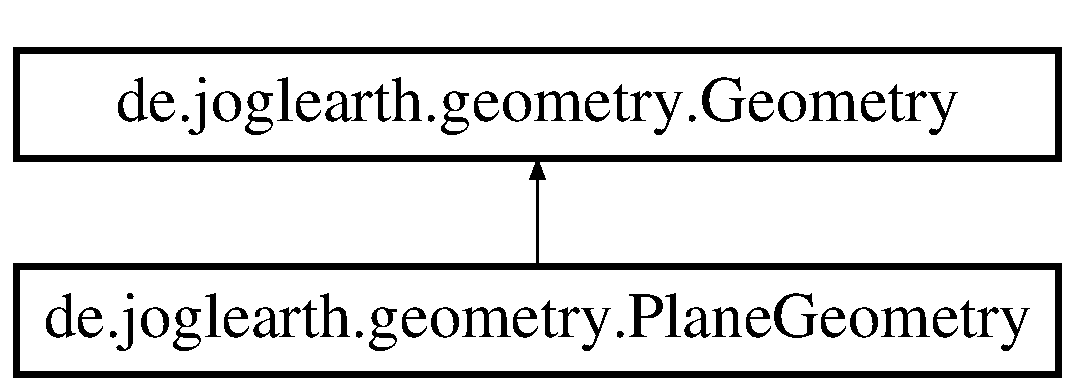
\includegraphics[height=2.000000cm]{classde_1_1joglearth_1_1geometry_1_1_plane_geometry}
\end{center}
\end{figure}
\subsection*{Öffentliche \-Methoden}
\begin{DoxyCompactItemize}
\item 
boolean {\bfseries is\-Point\-Visible} (float longitude, float latitude)\label{classde_1_1joglearth_1_1geometry_1_1_plane_geometry_a66a12f3965886a1488a658e046e726fd}

\item 
{\bf \-Vector3} {\bfseries get\-Space\-Position} (float longitude, float latitude)\label{classde_1_1joglearth_1_1geometry_1_1_plane_geometry_a14b781123b2815a789ed1120d2b4bdeb}

\item 
{\bf \-Screen\-Coordinates} {\bfseries get\-Surface\-Coordinates} ({\bf \-Vector3} view\-Vector)\label{classde_1_1joglearth_1_1geometry_1_1_plane_geometry_a75b2822c69800fb287274d37ec397784}

\item 
{\bf \-Matrix4} {\bfseries get\-View\-Matrix} ()\label{classde_1_1joglearth_1_1geometry_1_1_plane_geometry_a27f961bb318adbeec26f5cb930a35877}

\end{DoxyCompactItemize}

\section{de.\-joglearth.\-rendering.\-Plane\-Tessellator \-Klassenreferenz}
\label{classde_1_1joglearth_1_1rendering_1_1_plane_tessellator}\index{de.\-joglearth.\-rendering.\-Plane\-Tessellator@{de.\-joglearth.\-rendering.\-Plane\-Tessellator}}
\-Klassendiagramm für de.\-joglearth.\-rendering.\-Plane\-Tessellator\-:\begin{figure}[H]
\begin{center}
\leavevmode
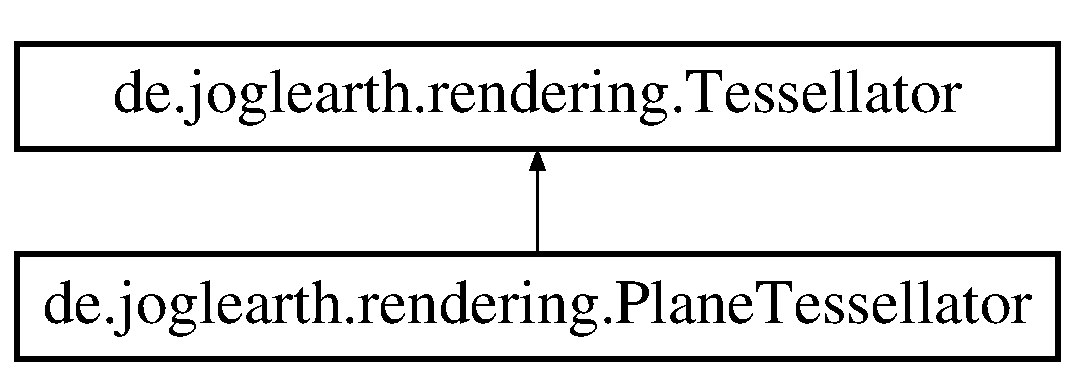
\includegraphics[height=2.000000cm]{classde_1_1joglearth_1_1rendering_1_1_plane_tessellator}
\end{center}
\end{figure}
\subsection*{Öffentliche \-Methoden}
\begin{DoxyCompactItemize}
\item 
{\bf \-Mesh} {\bf tessellate\-Tile} ({\bf \-Tile} tile, int subdivisions, {\bf \-Height\-Map\-Manager} height\-Map)
\end{DoxyCompactItemize}


\subsection{\-Ausführliche \-Beschreibung}
\-The {\ttfamily \-Plane\-Tesselator} calculates the \doxyref{\-Mesh}{\-S.}{classde_1_1joglearth_1_1rendering_1_1_mesh} for a \doxyref{de.\-joglearth.\-geometry.\-Tile}{\-S.}{classde_1_1joglearth_1_1geometry_1_1_tile} on a plane map. 

\subsection{\-Dokumentation der \-Elementfunktionen}
\index{de\-::joglearth\-::rendering\-::\-Plane\-Tessellator@{de\-::joglearth\-::rendering\-::\-Plane\-Tessellator}!tessellate\-Tile@{tessellate\-Tile}}
\index{tessellate\-Tile@{tessellate\-Tile}!de::joglearth::rendering::PlaneTessellator@{de\-::joglearth\-::rendering\-::\-Plane\-Tessellator}}
\subsubsection[{tessellate\-Tile}]{\setlength{\rightskip}{0pt plus 5cm}{\bf \-Mesh} {\bf de.\-joglearth.\-rendering.\-Plane\-Tessellator.\-tessellate\-Tile} (
\begin{DoxyParamCaption}
\item[{{\bf \-Tile}}]{tile, }
\item[{int}]{subdivisions, }
\item[{{\bf \-Height\-Map\-Manager}}]{height\-Map}
\end{DoxyParamCaption}
)}\label{classde_1_1joglearth_1_1rendering_1_1_plane_tessellator_ad8fb35a18af60f6285090669a6d41c52}

\begin{DoxyParams}{\-Parameter}
{\em tile} & \-The location where the \doxyref{\-Mesh}{\-S.}{classde_1_1joglearth_1_1rendering_1_1_mesh} should be rendered. \\
\hline
{\em subdivisions} & \-Number of times the \doxyref{\-Mesh}{\-S.}{classde_1_1joglearth_1_1rendering_1_1_mesh} is divided in both axis. \\
\hline
{\em height\-Map} & \-A \doxyref{de.\-joglearth.\-surface.\-Height\-Map\-Manager}{\-S.}{classde_1_1joglearth_1_1surface_1_1_height_map_manager} that provides the height data for the tile. \\
\hline
\end{DoxyParams}
\begin{DoxyReturn}{\-Rückgabe}
\-A \doxyref{\-Mesh}{\-S.}{classde_1_1joglearth_1_1rendering_1_1_mesh} with (subdivisions + 1)$^\wedge$2 squares, with each divided in two triangles. 
\end{DoxyReturn}


\-Implementiert {\bf de.\-joglearth.\-rendering.\-Tessellator} \doxyref{}{\-S.}{interfacede_1_1joglearth_1_1rendering_1_1_tessellator_a39d89f430ca5fab9912fe1db9c05e143}.


\section{de.\-joglearth.\-util.\-Predicate$<$ T $>$ Schnittstellenreferenz}
\label{interfacede_1_1joglearth_1_1util_1_1_predicate_3_01_t_01_4}\index{de.\-joglearth.\-util.\-Predicate$<$ T $>$@{de.\-joglearth.\-util.\-Predicate$<$ T $>$}}
\subsection*{Öffentliche Methoden}
\begin{DoxyCompactItemize}
\item 
boolean {\bfseries test} (T t)\label{interfacede_1_1joglearth_1_1util_1_1_predicate_3_01_t_01_4_ae9277408b5c3e3bab6ffe9f9c5064858}

\end{DoxyCompactItemize}

\section{de.\-joglearth.\-source.\-Progress\-Listener Schnittstellenreferenz}
\label{interfacede_1_1joglearth_1_1source_1_1_progress_listener}\index{de.\-joglearth.\-source.\-Progress\-Listener@{de.\-joglearth.\-source.\-Progress\-Listener}}
\subsection*{Öffentliche Methoden}
\begin{DoxyCompactItemize}
\item 
void {\bf update\-Progress} (double prog)
\item 
void {\bf abort\-Pending\-Requests} ()
\end{DoxyCompactItemize}


\subsection{Ausführliche Beschreibung}
Listener interface notified on \doxyref{Progress\-Manager}{S.}{classde_1_1joglearth_1_1source_1_1_progress_manager} events. 

\subsection{Dokumentation der Elementfunktionen}
\index{de\-::joglearth\-::source\-::\-Progress\-Listener@{de\-::joglearth\-::source\-::\-Progress\-Listener}!abort\-Pending\-Requests@{abort\-Pending\-Requests}}
\index{abort\-Pending\-Requests@{abort\-Pending\-Requests}!de::joglearth::source::ProgressListener@{de\-::joglearth\-::source\-::\-Progress\-Listener}}
\subsubsection[{abort\-Pending\-Requests}]{\setlength{\rightskip}{0pt plus 5cm}void de.\-joglearth.\-source.\-Progress\-Listener.\-abort\-Pending\-Requests (
\begin{DoxyParamCaption}
{}
\end{DoxyParamCaption}
)}\label{interfacede_1_1joglearth_1_1source_1_1_progress_listener_ae16476f3daec5f2d01844f2ff65738d9}
Is called when \doxyref{Progress\-Manager.\-abort\-Pending\-Requests()}{S.}{classde_1_1joglearth_1_1source_1_1_progress_manager_a1666689a11a8ed6d10605ece6bf4348d} is invoked. An implementation should attempt to stop any pending asynchronous request. \index{de\-::joglearth\-::source\-::\-Progress\-Listener@{de\-::joglearth\-::source\-::\-Progress\-Listener}!update\-Progress@{update\-Progress}}
\index{update\-Progress@{update\-Progress}!de::joglearth::source::ProgressListener@{de\-::joglearth\-::source\-::\-Progress\-Listener}}
\subsubsection[{update\-Progress}]{\setlength{\rightskip}{0pt plus 5cm}void de.\-joglearth.\-source.\-Progress\-Listener.\-update\-Progress (
\begin{DoxyParamCaption}
\item[{double}]{prog}
\end{DoxyParamCaption}
)}\label{interfacede_1_1joglearth_1_1source_1_1_progress_listener_a34023ed7363f7455d96e3a905c05f824}
Is called when the global loading progress changes.


\begin{DoxyParams}{Parameter}
{\em prog} & The progress, where 0.\-0 equals 0\% and 1.\-0 equals 100\% \\
\hline
\end{DoxyParams}

\section{de.\-joglearth.\-source.\-Progress\-Manager Klassenreferenz}
\label{classde_1_1joglearth_1_1source_1_1_progress_manager}\index{de.\-joglearth.\-source.\-Progress\-Manager@{de.\-joglearth.\-source.\-Progress\-Manager}}
\subsection*{Öffentliche Methoden}
\begin{DoxyCompactItemize}
\item 
synchronized void {\bf add\-Progress\-Listener} ({\bf Progress\-Listener} l)
\item 
synchronized void {\bf remove\-Progress\-Listener} ({\bf Progress\-Listener} l)
\item 
synchronized void {\bf abort\-Pending\-Requests} ()
\item 
synchronized void {\bf request\-Arrived} ()
\item 
synchronized void {\bf request\-Completed} ()
\end{DoxyCompactItemize}
\subsection*{Öffentliche, statische Methoden}
\begin{DoxyCompactItemize}
\item 
static synchronized {\bf Progress\-Manager} {\bf get\-Instance} ()
\end{DoxyCompactItemize}


\subsection{Ausführliche Beschreibung}
Singleton class managing the global progress of asynchronous requests handled by \doxyref{Request\-Distributor}{S.}{}s. 

\subsection{Dokumentation der Elementfunktionen}
\index{de\-::joglearth\-::source\-::\-Progress\-Manager@{de\-::joglearth\-::source\-::\-Progress\-Manager}!abort\-Pending\-Requests@{abort\-Pending\-Requests}}
\index{abort\-Pending\-Requests@{abort\-Pending\-Requests}!de::joglearth::source::ProgressManager@{de\-::joglearth\-::source\-::\-Progress\-Manager}}
\subsubsection[{abort\-Pending\-Requests}]{\setlength{\rightskip}{0pt plus 5cm}synchronized void de.\-joglearth.\-source.\-Progress\-Manager.\-abort\-Pending\-Requests (
\begin{DoxyParamCaption}
{}
\end{DoxyParamCaption}
)}\label{classde_1_1joglearth_1_1source_1_1_progress_manager_a1666689a11a8ed6d10605ece6bf4348d}
Removes all pending requests and notifies listeners that all remaining requests should be aborted. \index{de\-::joglearth\-::source\-::\-Progress\-Manager@{de\-::joglearth\-::source\-::\-Progress\-Manager}!add\-Progress\-Listener@{add\-Progress\-Listener}}
\index{add\-Progress\-Listener@{add\-Progress\-Listener}!de::joglearth::source::ProgressManager@{de\-::joglearth\-::source\-::\-Progress\-Manager}}
\subsubsection[{add\-Progress\-Listener}]{\setlength{\rightskip}{0pt plus 5cm}synchronized void de.\-joglearth.\-source.\-Progress\-Manager.\-add\-Progress\-Listener (
\begin{DoxyParamCaption}
\item[{{\bf Progress\-Listener}}]{l}
\end{DoxyParamCaption}
)}\label{classde_1_1joglearth_1_1source_1_1_progress_manager_af55cdcb08c0f04076d3d98ebdea11344}
Adds a new \doxyref{Progress\-Listener}{S.}{interfacede_1_1joglearth_1_1source_1_1_progress_listener} which is notified whenever the overall progress changes or the pending requests are to be aborted.


\begin{DoxyParams}{Parameter}
{\em l} & The listener to add. \\
\hline
\end{DoxyParams}
\index{de\-::joglearth\-::source\-::\-Progress\-Manager@{de\-::joglearth\-::source\-::\-Progress\-Manager}!get\-Instance@{get\-Instance}}
\index{get\-Instance@{get\-Instance}!de::joglearth::source::ProgressManager@{de\-::joglearth\-::source\-::\-Progress\-Manager}}
\subsubsection[{get\-Instance}]{\setlength{\rightskip}{0pt plus 5cm}static synchronized {\bf Progress\-Manager} de.\-joglearth.\-source.\-Progress\-Manager.\-get\-Instance (
\begin{DoxyParamCaption}
{}
\end{DoxyParamCaption}
)\hspace{0.3cm}{\ttfamily [static]}}\label{classde_1_1joglearth_1_1source_1_1_progress_manager_a31a505e4bbd05c02162356576b8dfae2}
Returns the instance of the singleton, creating it if it does not exist yet.

\begin{DoxyReturn}{Rückgabe}
The instance. 
\end{DoxyReturn}
\index{de\-::joglearth\-::source\-::\-Progress\-Manager@{de\-::joglearth\-::source\-::\-Progress\-Manager}!remove\-Progress\-Listener@{remove\-Progress\-Listener}}
\index{remove\-Progress\-Listener@{remove\-Progress\-Listener}!de::joglearth::source::ProgressManager@{de\-::joglearth\-::source\-::\-Progress\-Manager}}
\subsubsection[{remove\-Progress\-Listener}]{\setlength{\rightskip}{0pt plus 5cm}synchronized void de.\-joglearth.\-source.\-Progress\-Manager.\-remove\-Progress\-Listener (
\begin{DoxyParamCaption}
\item[{{\bf Progress\-Listener}}]{l}
\end{DoxyParamCaption}
)}\label{classde_1_1joglearth_1_1source_1_1_progress_manager_a4cffeb36cc57fbedad50b94c034924f5}
Removes an existing \doxyref{Progress\-Listener}{S.}{interfacede_1_1joglearth_1_1source_1_1_progress_listener} from the set of listeners.


\begin{DoxyParams}{Parameter}
{\em l} & The listener to remove. \\
\hline
\end{DoxyParams}
\index{de\-::joglearth\-::source\-::\-Progress\-Manager@{de\-::joglearth\-::source\-::\-Progress\-Manager}!request\-Arrived@{request\-Arrived}}
\index{request\-Arrived@{request\-Arrived}!de::joglearth::source::ProgressManager@{de\-::joglearth\-::source\-::\-Progress\-Manager}}
\subsubsection[{request\-Arrived}]{\setlength{\rightskip}{0pt plus 5cm}synchronized void de.\-joglearth.\-source.\-Progress\-Manager.\-request\-Arrived (
\begin{DoxyParamCaption}
{}
\end{DoxyParamCaption}
)}\label{classde_1_1joglearth_1_1source_1_1_progress_manager_a52cfde4a89f57ea4e446935c8e2a921f}
Adds a pending request, notifying all listeners of the change. \index{de\-::joglearth\-::source\-::\-Progress\-Manager@{de\-::joglearth\-::source\-::\-Progress\-Manager}!request\-Completed@{request\-Completed}}
\index{request\-Completed@{request\-Completed}!de::joglearth::source::ProgressManager@{de\-::joglearth\-::source\-::\-Progress\-Manager}}
\subsubsection[{request\-Completed}]{\setlength{\rightskip}{0pt plus 5cm}synchronized void de.\-joglearth.\-source.\-Progress\-Manager.\-request\-Completed (
\begin{DoxyParamCaption}
{}
\end{DoxyParamCaption}
)}\label{classde_1_1joglearth_1_1source_1_1_progress_manager_a930313dfc8f55932e8adc77cc7ad8615}
Marks a pending request as completed, notifying all listeners of the change. 
\section{de.\-joglearth.\-rendering.\-Renderer Klassenreferenz}
\label{classde_1_1joglearth_1_1rendering_1_1_renderer}\index{de.\-joglearth.\-rendering.\-Renderer@{de.\-joglearth.\-rendering.\-Renderer}}
\subsection*{Klassen}
\begin{DoxyCompactItemize}
\item 
class {\bfseries Graphics\-Settings\-Listener}
\item 
class {\bfseries Renderer\-Event\-Listener}
\item 
class {\bfseries Surface\-Validator}
\item 
class {\bfseries Worker}
\end{DoxyCompactItemize}
\subsection*{Öffentliche Methoden}
\begin{DoxyCompactItemize}
\item 
{\bf Renderer} (G\-L\-Canvas canv, {\bf Location\-Manager} location\-Manager, {\bf Camera} camera)
\item 
synchronized void {\bf post} ()
\item 
synchronized void {\bf start} ()
\item 
synchronized void {\bf stop} ()
\item 
void {\bf quit} ()
\item 
void {\bf set\-Display\-Mode} ({\bf Display\-Mode} m)
\item 
void {\bf set\-Map\-Type} ({\bf Single\-Map\-Type} t)
\item 
void {\bf set\-Map\-Type} ({\bf Tiled\-Map\-Type} t)
\end{DoxyCompactItemize}


\subsection{Ausführliche Beschreibung}
Handles the Open\-G\-L rendering. 

\subsection{Beschreibung der Konstruktoren und Destruktoren}
\index{de\-::joglearth\-::rendering\-::\-Renderer@{de\-::joglearth\-::rendering\-::\-Renderer}!Renderer@{Renderer}}
\index{Renderer@{Renderer}!de::joglearth::rendering::Renderer@{de\-::joglearth\-::rendering\-::\-Renderer}}
\subsubsection[{Renderer}]{\setlength{\rightskip}{0pt plus 5cm}de.\-joglearth.\-rendering.\-Renderer.\-Renderer (
\begin{DoxyParamCaption}
\item[{G\-L\-Canvas}]{canv, }
\item[{{\bf Location\-Manager}}]{location\-Manager, }
\item[{{\bf Camera}}]{camera}
\end{DoxyParamCaption}
)}\label{classde_1_1joglearth_1_1rendering_1_1_renderer_a0433a060d86ee3f69e0c204743bd6a50}
Constructor initializes the Open\-G\-L functionalities.


\begin{DoxyParams}{Parameter}
{\em canv} & G\-L\-Canvas object of the G\-U\-I \\
\hline
{\em height} & \doxyref{Height\-Map}{S.}{} that provides the height of a point \\
\hline
{\em location\-Manager} & \doxyref{Location\-Manager}{S.}{} that provides the information about Overlays to be displayed \\
\hline
{\em camera} & \doxyref{Camera}{S.}{} object \\
\hline
\end{DoxyParams}


\subsection{Dokumentation der Elementfunktionen}
\index{de\-::joglearth\-::rendering\-::\-Renderer@{de\-::joglearth\-::rendering\-::\-Renderer}!post@{post}}
\index{post@{post}!de::joglearth::rendering::Renderer@{de\-::joglearth\-::rendering\-::\-Renderer}}
\subsubsection[{post}]{\setlength{\rightskip}{0pt plus 5cm}synchronized void de.\-joglearth.\-rendering.\-Renderer.\-post (
\begin{DoxyParamCaption}
{}
\end{DoxyParamCaption}
)}\label{classde_1_1joglearth_1_1rendering_1_1_renderer_acdb2dda06a8744cb5f7975219a40a4f3}
Notifies the \doxyref{Renderer}{S.}{classde_1_1joglearth_1_1rendering_1_1_renderer} that a new frame should be rendered. If {\ttfamily \doxyref{start()}{S.}{classde_1_1joglearth_1_1rendering_1_1_renderer_ab112c71a1f00a287f343e896c950dc37}} is called this method may have no effect. Asynchronous method, does not wait until a frame is drawn. \index{de\-::joglearth\-::rendering\-::\-Renderer@{de\-::joglearth\-::rendering\-::\-Renderer}!quit@{quit}}
\index{quit@{quit}!de::joglearth::rendering::Renderer@{de\-::joglearth\-::rendering\-::\-Renderer}}
\subsubsection[{quit}]{\setlength{\rightskip}{0pt plus 5cm}void de.\-joglearth.\-rendering.\-Renderer.\-quit (
\begin{DoxyParamCaption}
{}
\end{DoxyParamCaption}
)}\label{classde_1_1joglearth_1_1rendering_1_1_renderer_afb25dedb47ab7ae5c0e326302c8e2a5c}
Quits the \doxyref{Renderer}{S.}{classde_1_1joglearth_1_1rendering_1_1_renderer} thread. \index{de\-::joglearth\-::rendering\-::\-Renderer@{de\-::joglearth\-::rendering\-::\-Renderer}!set\-Display\-Mode@{set\-Display\-Mode}}
\index{set\-Display\-Mode@{set\-Display\-Mode}!de::joglearth::rendering::Renderer@{de\-::joglearth\-::rendering\-::\-Renderer}}
\subsubsection[{set\-Display\-Mode}]{\setlength{\rightskip}{0pt plus 5cm}void de.\-joglearth.\-rendering.\-Renderer.\-set\-Display\-Mode (
\begin{DoxyParamCaption}
\item[{{\bf Display\-Mode}}]{m}
\end{DoxyParamCaption}
)}\label{classde_1_1joglearth_1_1rendering_1_1_renderer_a8ec4f320e1f8964b6569f37ff6ef42ba}
Sets the \doxyref{Display\-Mode}{S.}{enumde_1_1joglearth_1_1rendering_1_1_display_mode} to a given value.


\begin{DoxyParams}{Parameter}
{\em m} & The new {\ttfamily \doxyref{Display\-Mode}{S.}{enumde_1_1joglearth_1_1rendering_1_1_display_mode}} \\
\hline
\end{DoxyParams}
\index{de\-::joglearth\-::rendering\-::\-Renderer@{de\-::joglearth\-::rendering\-::\-Renderer}!set\-Map\-Type@{set\-Map\-Type}}
\index{set\-Map\-Type@{set\-Map\-Type}!de::joglearth::rendering::Renderer@{de\-::joglearth\-::rendering\-::\-Renderer}}
\subsubsection[{set\-Map\-Type}]{\setlength{\rightskip}{0pt plus 5cm}void de.\-joglearth.\-rendering.\-Renderer.\-set\-Map\-Type (
\begin{DoxyParamCaption}
\item[{{\bf Single\-Map\-Type}}]{t}
\end{DoxyParamCaption}
)}\label{classde_1_1joglearth_1_1rendering_1_1_renderer_a6dfc0ad658ba63b0eac647397aad7704}
Sets the \doxyref{Map\-Layout}{S.}{} to a given value. This type is a \doxyref{Single\-Map\-Type}{S.}{} as it is only one tile as a texture.


\begin{DoxyParams}{Parameter}
{\em t} & The new {\ttfamily Map\-Layout} \\
\hline
\end{DoxyParams}
\index{de\-::joglearth\-::rendering\-::\-Renderer@{de\-::joglearth\-::rendering\-::\-Renderer}!set\-Map\-Type@{set\-Map\-Type}}
\index{set\-Map\-Type@{set\-Map\-Type}!de::joglearth::rendering::Renderer@{de\-::joglearth\-::rendering\-::\-Renderer}}
\subsubsection[{set\-Map\-Type}]{\setlength{\rightskip}{0pt plus 5cm}void de.\-joglearth.\-rendering.\-Renderer.\-set\-Map\-Type (
\begin{DoxyParamCaption}
\item[{{\bf Tiled\-Map\-Type}}]{t}
\end{DoxyParamCaption}
)}\label{classde_1_1joglearth_1_1rendering_1_1_renderer_a968c90cff4efe05abcacf346fd3fd48d}
Sets the \doxyref{Map\-Layout}{S.}{} to a given value. This type is a \doxyref{Tiled\-Map\-Type}{S.}{} as the texture consists of multiple tiles.


\begin{DoxyParams}{Parameter}
{\em t} & The new {\ttfamily Map\-Layout} \\
\hline
\end{DoxyParams}
\index{de\-::joglearth\-::rendering\-::\-Renderer@{de\-::joglearth\-::rendering\-::\-Renderer}!start@{start}}
\index{start@{start}!de::joglearth::rendering::Renderer@{de\-::joglearth\-::rendering\-::\-Renderer}}
\subsubsection[{start}]{\setlength{\rightskip}{0pt plus 5cm}synchronized void de.\-joglearth.\-rendering.\-Renderer.\-start (
\begin{DoxyParamCaption}
{}
\end{DoxyParamCaption}
)}\label{classde_1_1joglearth_1_1rendering_1_1_renderer_ab112c71a1f00a287f343e896c950dc37}
Starts the render loop with 60 F\-P\-S. \index{de\-::joglearth\-::rendering\-::\-Renderer@{de\-::joglearth\-::rendering\-::\-Renderer}!stop@{stop}}
\index{stop@{stop}!de::joglearth::rendering::Renderer@{de\-::joglearth\-::rendering\-::\-Renderer}}
\subsubsection[{stop}]{\setlength{\rightskip}{0pt plus 5cm}synchronized void de.\-joglearth.\-rendering.\-Renderer.\-stop (
\begin{DoxyParamCaption}
{}
\end{DoxyParamCaption}
)}\label{classde_1_1joglearth_1_1rendering_1_1_renderer_abc1949c3ee8ccea9a14c299a969017cd}
Stops the render loop. When {\ttfamily \doxyref{post()}{S.}{classde_1_1joglearth_1_1rendering_1_1_renderer_acdb2dda06a8744cb5f7975219a40a4f3}} is called a new frame will be rendered. 
\section{de.\-joglearth.\-source.\-caching.\-Request\-Distributor$<$ Key, Value $>$ Klassenreferenz}
\label{classde_1_1joglearth_1_1source_1_1caching_1_1_request_distributor_3_01_key_00_01_value_01_4}\index{de.\-joglearth.\-source.\-caching.\-Request\-Distributor$<$ Key, Value $>$@{de.\-joglearth.\-source.\-caching.\-Request\-Distributor$<$ Key, Value $>$}}


Abgeleitet von Source$<$ Key, Value $>$.

\subsection*{Klassen}
\begin{DoxyCompactItemize}
\item 
class {\bfseries Cache\-Entry}
\item 
class {\bfseries Cache\-Handle}
\item 
class {\bfseries Cache\-Listener}
\end{DoxyCompactItemize}
\subsection*{Öffentliche Methoden}
\begin{DoxyCompactItemize}
\item 
void {\bf add\-Cache} (Cache$<$ Key, Value $>$ cache, int max\-Size)
\item 
void {\bf set\-Cache\-Size} (Cache$<$ Key, Value $>$ cache, int max\-Size)
\item 
void {\bf set\-Source} (Source$<$ Key, Value $>$ source)
\item 
Source\-Response$<$ Value $>$ {\bf request\-Object} (Key key, Source\-Listener$<$ Key, Value $>$ sender)
\item 
{\bf Request\-Distributor} (Object\-Measure$<$ Value $>$ m)
\item 
{\bf Request\-Distributor} ()
\item 
void {\bf drop\-All} ()
\item 
void {\bf drop\-All} (Predicate$<$ Key $>$ pred)
\item 
void {\bf drop\-Object} (Key k)
\end{DoxyCompactItemize}


\subsection{Ausführliche Beschreibung}
Dispatches requests for objects to a number of caches and an underlying source.

Retrieved objects are moved to faster caches after access, thus optimizing the response time for repeating queries. 

\subsection{Beschreibung der Konstruktoren und Destruktoren}
\index{de\-::joglearth\-::source\-::caching\-::\-Request\-Distributor$<$ Key, Value $>$@{de\-::joglearth\-::source\-::caching\-::\-Request\-Distributor$<$ Key, Value $>$}!Request\-Distributor@{Request\-Distributor}}
\index{Request\-Distributor@{Request\-Distributor}!de::joglearth::source::caching::RequestDistributor< Key, Value >@{de\-::joglearth\-::source\-::caching\-::\-Request\-Distributor$<$ Key, Value $>$}}
\subsubsection[{Request\-Distributor}]{\setlength{\rightskip}{0pt plus 5cm}de.\-joglearth.\-source.\-caching.\-Request\-Distributor$<$ Key, Value $>$.Request\-Distributor (
\begin{DoxyParamCaption}
\item[{Object\-Measure$<$ Value $>$}]{m}
\end{DoxyParamCaption}
)}\label{classde_1_1joglearth_1_1source_1_1caching_1_1_request_distributor_3_01_key_00_01_value_01_4_a356575251551009739db3a8b7a172eda}
Constructor.


\begin{DoxyParams}{Parameter}
{\em m} & The \doxyref{Object\-Measure}{S.}{} to use \\
\hline
\end{DoxyParams}
\index{de\-::joglearth\-::source\-::caching\-::\-Request\-Distributor$<$ Key, Value $>$@{de\-::joglearth\-::source\-::caching\-::\-Request\-Distributor$<$ Key, Value $>$}!Request\-Distributor@{Request\-Distributor}}
\index{Request\-Distributor@{Request\-Distributor}!de::joglearth::source::caching::RequestDistributor< Key, Value >@{de\-::joglearth\-::source\-::caching\-::\-Request\-Distributor$<$ Key, Value $>$}}
\subsubsection[{Request\-Distributor}]{\setlength{\rightskip}{0pt plus 5cm}de.\-joglearth.\-source.\-caching.\-Request\-Distributor$<$ Key, Value $>$.Request\-Distributor (
\begin{DoxyParamCaption}
{}
\end{DoxyParamCaption}
)}\label{classde_1_1joglearth_1_1source_1_1caching_1_1_request_distributor_3_01_key_00_01_value_01_4_a2951a2de7bb7e752b1570991d3419ad4}
Default constructor. Uses \doxyref{Unity\-Measure}{S.}{} as \doxyref{Object\-Measure}{S.}{}. 

\subsection{Dokumentation der Elementfunktionen}
\index{de\-::joglearth\-::source\-::caching\-::\-Request\-Distributor$<$ Key, Value $>$@{de\-::joglearth\-::source\-::caching\-::\-Request\-Distributor$<$ Key, Value $>$}!add\-Cache@{add\-Cache}}
\index{add\-Cache@{add\-Cache}!de::joglearth::source::caching::RequestDistributor< Key, Value >@{de\-::joglearth\-::source\-::caching\-::\-Request\-Distributor$<$ Key, Value $>$}}
\subsubsection[{add\-Cache}]{\setlength{\rightskip}{0pt plus 5cm}void de.\-joglearth.\-source.\-caching.\-Request\-Distributor$<$ Key, Value $>$.add\-Cache (
\begin{DoxyParamCaption}
\item[{Cache$<$ Key, Value $>$}]{cache, }
\item[{int}]{max\-Size}
\end{DoxyParamCaption}
)}\label{classde_1_1joglearth_1_1source_1_1caching_1_1_request_distributor_3_01_key_00_01_value_01_4_a18da9721a25e75be8bb654c461a4c45d}
Appends a new cache, which will have the lowest priority of any cache added so far.


\begin{DoxyParams}{Parameter}
{\em cache} & The cache \\
\hline
{\em max\-Size} & The maximum size in units defined by the Object\-Measure passed in the constructor, has to be greater than {\ttfamily 0} \\
\hline
\end{DoxyParams}
\index{de\-::joglearth\-::source\-::caching\-::\-Request\-Distributor$<$ Key, Value $>$@{de\-::joglearth\-::source\-::caching\-::\-Request\-Distributor$<$ Key, Value $>$}!drop\-All@{drop\-All}}
\index{drop\-All@{drop\-All}!de::joglearth::source::caching::RequestDistributor< Key, Value >@{de\-::joglearth\-::source\-::caching\-::\-Request\-Distributor$<$ Key, Value $>$}}
\subsubsection[{drop\-All}]{\setlength{\rightskip}{0pt plus 5cm}void de.\-joglearth.\-source.\-caching.\-Request\-Distributor$<$ Key, Value $>$.drop\-All (
\begin{DoxyParamCaption}
{}
\end{DoxyParamCaption}
)}\label{classde_1_1joglearth_1_1source_1_1caching_1_1_request_distributor_3_01_key_00_01_value_01_4_abf8c409b311e0888dd36dbca3c3dd6ae}
Drops all cached objects. \index{de\-::joglearth\-::source\-::caching\-::\-Request\-Distributor$<$ Key, Value $>$@{de\-::joglearth\-::source\-::caching\-::\-Request\-Distributor$<$ Key, Value $>$}!drop\-All@{drop\-All}}
\index{drop\-All@{drop\-All}!de::joglearth::source::caching::RequestDistributor< Key, Value >@{de\-::joglearth\-::source\-::caching\-::\-Request\-Distributor$<$ Key, Value $>$}}
\subsubsection[{drop\-All}]{\setlength{\rightskip}{0pt plus 5cm}void de.\-joglearth.\-source.\-caching.\-Request\-Distributor$<$ Key, Value $>$.drop\-All (
\begin{DoxyParamCaption}
\item[{Predicate$<$ Key $>$}]{pred}
\end{DoxyParamCaption}
)}\label{classde_1_1joglearth_1_1source_1_1caching_1_1_request_distributor_3_01_key_00_01_value_01_4_a9f5c4e8442dad9a5c1f2a9de21fcc13f}
Removes all objects from the \doxyref{cache}{S.}{}s that fulfill the \doxyref{Predicate}{S.}{}.


\begin{DoxyParams}{Parameter}
{\em pred} & Conformance with that {\ttfamily Predicate} leads to deletion of that object \\
\hline
\end{DoxyParams}
\index{de\-::joglearth\-::source\-::caching\-::\-Request\-Distributor$<$ Key, Value $>$@{de\-::joglearth\-::source\-::caching\-::\-Request\-Distributor$<$ Key, Value $>$}!drop\-Object@{drop\-Object}}
\index{drop\-Object@{drop\-Object}!de::joglearth::source::caching::RequestDistributor< Key, Value >@{de\-::joglearth\-::source\-::caching\-::\-Request\-Distributor$<$ Key, Value $>$}}
\subsubsection[{drop\-Object}]{\setlength{\rightskip}{0pt plus 5cm}void de.\-joglearth.\-source.\-caching.\-Request\-Distributor$<$ Key, Value $>$.drop\-Object (
\begin{DoxyParamCaption}
\item[{Key}]{k}
\end{DoxyParamCaption}
)}\label{classde_1_1joglearth_1_1source_1_1caching_1_1_request_distributor_3_01_key_00_01_value_01_4_a5e40a92cd0440bb2d6ab372e4c718cf4}
Removes an object stored under a {\ttfamily Key} from the \doxyref{Cache}{S.}{} that contains it.


\begin{DoxyParams}{Parameter}
{\em k} & The key identifying the object \\
\hline
\end{DoxyParams}
\index{de\-::joglearth\-::source\-::caching\-::\-Request\-Distributor$<$ Key, Value $>$@{de\-::joglearth\-::source\-::caching\-::\-Request\-Distributor$<$ Key, Value $>$}!request\-Object@{request\-Object}}
\index{request\-Object@{request\-Object}!de::joglearth::source::caching::RequestDistributor< Key, Value >@{de\-::joglearth\-::source\-::caching\-::\-Request\-Distributor$<$ Key, Value $>$}}
\subsubsection[{request\-Object}]{\setlength{\rightskip}{0pt plus 5cm}Source\-Response$<$Value$>$ de.\-joglearth.\-source.\-caching.\-Request\-Distributor$<$ Key, Value $>$.request\-Object (
\begin{DoxyParamCaption}
\item[{Key}]{key, }
\item[{Source\-Listener$<$ Key, Value $>$}]{sender}
\end{DoxyParamCaption}
)}\label{classde_1_1joglearth_1_1source_1_1caching_1_1_request_distributor_3_01_key_00_01_value_01_4_a0dddf19cb7d3f9a9664b7dad36816d89}
Tries to retrieve a requested object. Asks \doxyref{Cache}{S.}{}s in the order of their hierarchy, if the object is not in the {\ttfamily Caches} it asks its \doxyref{Source}{S.}{}. Objects that are not found in the primary {\ttfamily Cache}, but in another {\ttfamily Cache} or the {\ttfamily Source} are stored in the primary {\ttfamily Cache}. This may lead to displacements of other objects from the primary {\ttfamily Cache}.


\begin{DoxyParams}{Parameter}
{\em key} & Identifier of the requested object \\
\hline
{\em sender} & Entity to be notified when request is completed asynchronous \\
\hline
\end{DoxyParams}
\index{de\-::joglearth\-::source\-::caching\-::\-Request\-Distributor$<$ Key, Value $>$@{de\-::joglearth\-::source\-::caching\-::\-Request\-Distributor$<$ Key, Value $>$}!set\-Cache\-Size@{set\-Cache\-Size}}
\index{set\-Cache\-Size@{set\-Cache\-Size}!de::joglearth::source::caching::RequestDistributor< Key, Value >@{de\-::joglearth\-::source\-::caching\-::\-Request\-Distributor$<$ Key, Value $>$}}
\subsubsection[{set\-Cache\-Size}]{\setlength{\rightskip}{0pt plus 5cm}void de.\-joglearth.\-source.\-caching.\-Request\-Distributor$<$ Key, Value $>$.set\-Cache\-Size (
\begin{DoxyParamCaption}
\item[{Cache$<$ Key, Value $>$}]{cache, }
\item[{int}]{max\-Size}
\end{DoxyParamCaption}
)}\label{classde_1_1joglearth_1_1source_1_1caching_1_1_request_distributor_3_01_key_00_01_value_01_4_a9f434cffad6e2b3f6f085a3c42568e91}
Changes the maximum size of an existing cache, possibly dropping cached objects in the process.


\begin{DoxyParams}{Parameter}
{\em cache} & The cache to modify \\
\hline
{\em max\-Size} & The new maximum size, has to be greater than {\ttfamily 0} \\
\hline
\end{DoxyParams}
\index{de\-::joglearth\-::source\-::caching\-::\-Request\-Distributor$<$ Key, Value $>$@{de\-::joglearth\-::source\-::caching\-::\-Request\-Distributor$<$ Key, Value $>$}!set\-Source@{set\-Source}}
\index{set\-Source@{set\-Source}!de::joglearth::source::caching::RequestDistributor< Key, Value >@{de\-::joglearth\-::source\-::caching\-::\-Request\-Distributor$<$ Key, Value $>$}}
\subsubsection[{set\-Source}]{\setlength{\rightskip}{0pt plus 5cm}void de.\-joglearth.\-source.\-caching.\-Request\-Distributor$<$ Key, Value $>$.set\-Source (
\begin{DoxyParamCaption}
\item[{Source$<$ Key, Value $>$}]{source}
\end{DoxyParamCaption}
)}\label{classde_1_1joglearth_1_1source_1_1caching_1_1_request_distributor_3_01_key_00_01_value_01_4_a2961584cee25c3101f7bd849e3bfa6f0}
Replaces the \doxyref{Source}{S.}{}.


\begin{DoxyParams}{Parameter}
{\em source} & The new source \\
\hline
\end{DoxyParams}

\section{de.\-joglearth.\-util.\-Resource Klassenreferenz}
\label{classde_1_1joglearth_1_1util_1_1_resource}\index{de.\-joglearth.\-util.\-Resource@{de.\-joglearth.\-util.\-Resource}}
\subsection*{Öffentliche, statische Methoden}
\begin{DoxyCompactItemize}
\item 
static Image\-Icon {\bf load\-Icon} (String name)
\end{DoxyCompactItemize}


\subsection{Ausführliche Beschreibung}
Utility class for loading data from J\-A\-R resources file. 

\subsection{Dokumentation der Elementfunktionen}
\index{de\-::joglearth\-::util\-::\-Resource@{de\-::joglearth\-::util\-::\-Resource}!load\-Icon@{load\-Icon}}
\index{load\-Icon@{load\-Icon}!de::joglearth::util::Resource@{de\-::joglearth\-::util\-::\-Resource}}
\subsubsection[{load\-Icon}]{\setlength{\rightskip}{0pt plus 5cm}static Image\-Icon de.\-joglearth.\-util.\-Resource.\-load\-Icon (
\begin{DoxyParamCaption}
\item[{String}]{name}
\end{DoxyParamCaption}
)\hspace{0.3cm}{\ttfamily [static]}}\label{classde_1_1joglearth_1_1util_1_1_resource_a0a34e861a5a69284adae6f72c4d2f16e}
Loads a Swing {\ttfamily Image\-Icon} from an image resource. 
\begin{DoxyParams}{Parameter}
{\em name} & The resource file name \\
\hline
\end{DoxyParams}
\begin{DoxyReturn}{Rückgabe}
The icon if successfully loaded, else {\ttfamily null} 
\end{DoxyReturn}

\section{de.\-joglearth.\-geometry.\-Screen\-Coordinates \-Klassenreferenz}
\label{classde_1_1joglearth_1_1geometry_1_1_screen_coordinates}\index{de.\-joglearth.\-geometry.\-Screen\-Coordinates@{de.\-joglearth.\-geometry.\-Screen\-Coordinates}}
\subsection*{Öffentliche \-Methoden}
\begin{DoxyCompactItemize}
\item 
{\bfseries \-Screen\-Coordinates} (float x, float y)\label{classde_1_1joglearth_1_1geometry_1_1_screen_coordinates_afc87532187738efd163d3e42981c3aaa}

\item 
{\bf \-Screen\-Coordinates} {\bfseries clone} ()\label{classde_1_1joglearth_1_1geometry_1_1_screen_coordinates_a331deb737a91c46e453ea2ea1639ca0e}

\end{DoxyCompactItemize}
\subsection*{Öffentliche \-Attribute}
\begin{DoxyCompactItemize}
\item 
float {\bfseries x}\label{classde_1_1joglearth_1_1geometry_1_1_screen_coordinates_ac92e209f6e5cdc4576c2f78084429aed}

\item 
float {\bfseries y}\label{classde_1_1joglearth_1_1geometry_1_1_screen_coordinates_a3916869098772aa49552deae6aa0e1cc}

\end{DoxyCompactItemize}

\section{de.\-joglearth.\-settings.\-Settings Klassenreferenz}
\label{classde_1_1joglearth_1_1settings_1_1_settings}\index{de.\-joglearth.\-settings.\-Settings@{de.\-joglearth.\-settings.\-Settings}}
\subsection*{Öffentliche Methoden}
\begin{DoxyCompactItemize}
\item 
void {\bf add\-Settings\-Listener} (final String key, final {\bf Settings\-Listener} listener)
\item 
void {\bf remove\-Settings\-Listener} (final String key, final {\bf Settings\-Listener} listener)
\item 
synchronized void {\bf put\-Integer} (final String key, final Integer value)
\item 
synchronized void {\bf put\-Double} (final String key, final Double value)
\item 
synchronized void {\bf put\-Float} (final String key, final Float value)
\item 
synchronized void {\bf put\-Long} (final String key, final Long value)
\item 
synchronized void {\bf put\-Location} (final String key, final {\bf Location} value)
\item 
synchronized void {\bf drop\-Location} (final String key, final {\bf Location} value)
\item 
synchronized void {\bf put\-Boolean} (final String key, final Boolean value)
\item 
synchronized void {\bf put\-String} (final String key, final String value)
\item 
synchronized Boolean {\bf get\-Boolean} (final String key)
\item 
synchronized String {\bf get\-String} (final String key)
\item 
synchronized Long {\bf get\-Long} (final String key)
\item 
synchronized Float {\bf get\-Float} (final String key)
\item 
synchronized Double {\bf get\-Double} (final String key)
\item 
synchronized Integer {\bf get\-Integer} (final String key)
\item 
synchronized Set$<$ {\bf Location} $>$ {\bf get\-Locations} (final String key)
\end{DoxyCompactItemize}
\subsection*{Öffentliche, statische Methoden}
\begin{DoxyCompactItemize}
\item 
static synchronized {\bf Settings} {\bf get\-Instance} ()
\end{DoxyCompactItemize}


\subsection{Ausführliche Beschreibung}
Used to store settings of \doxyref{Jogl\-Earth}{S.}{classde_1_1joglearth_1_1_jogl_earth}. A key can only have one value, except for Locations where multiple can exist under the same key. If put a value of an other type under the same key it replaces the old value of the other type. For key the {\ttfamily null} object is not allowed. This class is thread-\/safe. 

\subsection{Dokumentation der Elementfunktionen}
\index{de\-::joglearth\-::settings\-::\-Settings@{de\-::joglearth\-::settings\-::\-Settings}!add\-Settings\-Listener@{add\-Settings\-Listener}}
\index{add\-Settings\-Listener@{add\-Settings\-Listener}!de::joglearth::settings::Settings@{de\-::joglearth\-::settings\-::\-Settings}}
\subsubsection[{add\-Settings\-Listener}]{\setlength{\rightskip}{0pt plus 5cm}void de.\-joglearth.\-settings.\-Settings.\-add\-Settings\-Listener (
\begin{DoxyParamCaption}
\item[{final String}]{key, }
\item[{final {\bf Settings\-Listener}}]{listener}
\end{DoxyParamCaption}
)}\label{classde_1_1joglearth_1_1settings_1_1_settings_acf7129cfcc147ae7729ce2bad966e04e}
Add a \doxyref{Settings\-Listener}{S.}{interfacede_1_1joglearth_1_1settings_1_1_settings_listener} to be called if the setting with the given name is changed.


\begin{DoxyParams}{Parameter}
{\em key} & The key of the setting \\
\hline
{\em listener} & The listener to be called \\
\hline
\end{DoxyParams}
\index{de\-::joglearth\-::settings\-::\-Settings@{de\-::joglearth\-::settings\-::\-Settings}!drop\-Location@{drop\-Location}}
\index{drop\-Location@{drop\-Location}!de::joglearth::settings::Settings@{de\-::joglearth\-::settings\-::\-Settings}}
\subsubsection[{drop\-Location}]{\setlength{\rightskip}{0pt plus 5cm}synchronized void de.\-joglearth.\-settings.\-Settings.\-drop\-Location (
\begin{DoxyParamCaption}
\item[{final String}]{key, }
\item[{final {\bf Location}}]{value}
\end{DoxyParamCaption}
)}\label{classde_1_1joglearth_1_1settings_1_1_settings_a93f664ab93cb83d852b98a400a1e4c11}
Removes the given \doxyref{Location}{S.}{} from the given key. The Location that is removed is found by the {\ttfamily this == value $|$$|$ this.\-equals(value)}


\begin{DoxyParams}{Parameter}
{\em key} & the key the {\ttfamily Location} should be removed from \\
\hline
{\em value} & the {\ttfamily Location} to remove \\
\hline
\end{DoxyParams}
\index{de\-::joglearth\-::settings\-::\-Settings@{de\-::joglearth\-::settings\-::\-Settings}!get\-Boolean@{get\-Boolean}}
\index{get\-Boolean@{get\-Boolean}!de::joglearth::settings::Settings@{de\-::joglearth\-::settings\-::\-Settings}}
\subsubsection[{get\-Boolean}]{\setlength{\rightskip}{0pt plus 5cm}synchronized Boolean de.\-joglearth.\-settings.\-Settings.\-get\-Boolean (
\begin{DoxyParamCaption}
\item[{final String}]{key}
\end{DoxyParamCaption}
)}\label{classde_1_1joglearth_1_1settings_1_1_settings_a6e3d0defd993ace2d60feaeb0bd11c85}
Retrieve the setting stored, using the given key, as {\ttfamily Boolean} .


\begin{DoxyParams}{Parameter}
{\em key} & The key of the setting \\
\hline
\end{DoxyParams}
\begin{DoxyReturn}{Rückgabe}
The setting stored under the given key as {\ttfamily Boolean} or {\ttfamily null} if no setting found with given name or the setting is no instance of {\ttfamily Boolean} 
\end{DoxyReturn}
\index{de\-::joglearth\-::settings\-::\-Settings@{de\-::joglearth\-::settings\-::\-Settings}!get\-Double@{get\-Double}}
\index{get\-Double@{get\-Double}!de::joglearth::settings::Settings@{de\-::joglearth\-::settings\-::\-Settings}}
\subsubsection[{get\-Double}]{\setlength{\rightskip}{0pt plus 5cm}synchronized Double de.\-joglearth.\-settings.\-Settings.\-get\-Double (
\begin{DoxyParamCaption}
\item[{final String}]{key}
\end{DoxyParamCaption}
)}\label{classde_1_1joglearth_1_1settings_1_1_settings_a8416ad653d1b524486c9f7af450535d6}
Retrieve the setting stored, using the given key, as {\ttfamily Double}.


\begin{DoxyParams}{Parameter}
{\em key} & The key of the setting \\
\hline
\end{DoxyParams}
\begin{DoxyReturn}{Rückgabe}
The setting stored under the given key as {\ttfamily Double} or {\ttfamily null} if no setting found with given name or the setting is no instance of {\ttfamily Double} 
\end{DoxyReturn}
\index{de\-::joglearth\-::settings\-::\-Settings@{de\-::joglearth\-::settings\-::\-Settings}!get\-Float@{get\-Float}}
\index{get\-Float@{get\-Float}!de::joglearth::settings::Settings@{de\-::joglearth\-::settings\-::\-Settings}}
\subsubsection[{get\-Float}]{\setlength{\rightskip}{0pt plus 5cm}synchronized Float de.\-joglearth.\-settings.\-Settings.\-get\-Float (
\begin{DoxyParamCaption}
\item[{final String}]{key}
\end{DoxyParamCaption}
)}\label{classde_1_1joglearth_1_1settings_1_1_settings_a7b9b4f224da094ed2c0e581953fbbbcf}
Retrieve the setting stored, using the given key, as {\ttfamily Float}.


\begin{DoxyParams}{Parameter}
{\em key} & The key of the setting \\
\hline
\end{DoxyParams}
\begin{DoxyReturn}{Rückgabe}
The setting stored under the given key as {\ttfamily Float} or {\ttfamily null} if no setting found with given name or the setting is no instance of {\ttfamily Float} 
\end{DoxyReturn}
\index{de\-::joglearth\-::settings\-::\-Settings@{de\-::joglearth\-::settings\-::\-Settings}!get\-Instance@{get\-Instance}}
\index{get\-Instance@{get\-Instance}!de::joglearth::settings::Settings@{de\-::joglearth\-::settings\-::\-Settings}}
\subsubsection[{get\-Instance}]{\setlength{\rightskip}{0pt plus 5cm}static synchronized {\bf Settings} de.\-joglearth.\-settings.\-Settings.\-get\-Instance (
\begin{DoxyParamCaption}
{}
\end{DoxyParamCaption}
)\hspace{0.3cm}{\ttfamily [static]}}\label{classde_1_1joglearth_1_1settings_1_1_settings_a58ca604701da037a83b9e455cb7dc1f9}
Get the instance of \doxyref{Settings}{S.}{classde_1_1joglearth_1_1settings_1_1_settings}.

\begin{DoxyReturn}{Rückgabe}
The settings 
\end{DoxyReturn}
\index{de\-::joglearth\-::settings\-::\-Settings@{de\-::joglearth\-::settings\-::\-Settings}!get\-Integer@{get\-Integer}}
\index{get\-Integer@{get\-Integer}!de::joglearth::settings::Settings@{de\-::joglearth\-::settings\-::\-Settings}}
\subsubsection[{get\-Integer}]{\setlength{\rightskip}{0pt plus 5cm}synchronized Integer de.\-joglearth.\-settings.\-Settings.\-get\-Integer (
\begin{DoxyParamCaption}
\item[{final String}]{key}
\end{DoxyParamCaption}
)}\label{classde_1_1joglearth_1_1settings_1_1_settings_ad29c8250467949616b226df5df249d69}
Retrieve the setting stored, using the given key, as {\ttfamily Integer} .


\begin{DoxyParams}{Parameter}
{\em key} & The key of the setting \\
\hline
\end{DoxyParams}
\begin{DoxyReturn}{Rückgabe}
The setting stored under the given key as {\ttfamily Integer} or {\ttfamily null} if no setting found with given name or the setting is no instance of {\ttfamily Integer} 
\end{DoxyReturn}
\index{de\-::joglearth\-::settings\-::\-Settings@{de\-::joglearth\-::settings\-::\-Settings}!get\-Locations@{get\-Locations}}
\index{get\-Locations@{get\-Locations}!de::joglearth::settings::Settings@{de\-::joglearth\-::settings\-::\-Settings}}
\subsubsection[{get\-Locations}]{\setlength{\rightskip}{0pt plus 5cm}synchronized Set$<${\bf Location}$>$ de.\-joglearth.\-settings.\-Settings.\-get\-Locations (
\begin{DoxyParamCaption}
\item[{final String}]{key}
\end{DoxyParamCaption}
)}\label{classde_1_1joglearth_1_1settings_1_1_settings_a08cb9e5ada6ae8604cf3b8030daedb4e}
Gets the \doxyref{Location}{S.}{} Objects stored using the given key.


\begin{DoxyParams}{Parameter}
{\em key} & the key to use \\
\hline
\end{DoxyParams}
\begin{DoxyReturn}{Rückgabe}
a {\ttfamily Set} of {\ttfamily Location} Objects stored under the given key or {\ttfamily null} if no {\ttfamily Location} Object is found using this key. 
\end{DoxyReturn}
\index{de\-::joglearth\-::settings\-::\-Settings@{de\-::joglearth\-::settings\-::\-Settings}!get\-Long@{get\-Long}}
\index{get\-Long@{get\-Long}!de::joglearth::settings::Settings@{de\-::joglearth\-::settings\-::\-Settings}}
\subsubsection[{get\-Long}]{\setlength{\rightskip}{0pt plus 5cm}synchronized Long de.\-joglearth.\-settings.\-Settings.\-get\-Long (
\begin{DoxyParamCaption}
\item[{final String}]{key}
\end{DoxyParamCaption}
)}\label{classde_1_1joglearth_1_1settings_1_1_settings_a4d6b91a5b97e08d0aa4e42c4c73c60d8}
Retrieve the setting stored, using the given key, as {\ttfamily Long}.


\begin{DoxyParams}{Parameter}
{\em key} & The key of the setting \\
\hline
\end{DoxyParams}
\begin{DoxyReturn}{Rückgabe}
The setting stored under the given key as {\ttfamily Long} or {\ttfamily null} if no setting found with given name or the setting is no instance of {\ttfamily Long} 
\end{DoxyReturn}
\index{de\-::joglearth\-::settings\-::\-Settings@{de\-::joglearth\-::settings\-::\-Settings}!get\-String@{get\-String}}
\index{get\-String@{get\-String}!de::joglearth::settings::Settings@{de\-::joglearth\-::settings\-::\-Settings}}
\subsubsection[{get\-String}]{\setlength{\rightskip}{0pt plus 5cm}synchronized String de.\-joglearth.\-settings.\-Settings.\-get\-String (
\begin{DoxyParamCaption}
\item[{final String}]{key}
\end{DoxyParamCaption}
)}\label{classde_1_1joglearth_1_1settings_1_1_settings_a2dd7edb036f43fc18c43abccf7dcc0dc}
Retrieve the setting stored, using the given key, as {\ttfamily String}.


\begin{DoxyParams}{Parameter}
{\em key} & The key of the setting \\
\hline
\end{DoxyParams}
\begin{DoxyReturn}{Rückgabe}
The setting stored under the given key as String or {\ttfamily null} if no setting found with given name or the setting is no instance of {\ttfamily String} 
\end{DoxyReturn}
\index{de\-::joglearth\-::settings\-::\-Settings@{de\-::joglearth\-::settings\-::\-Settings}!put\-Boolean@{put\-Boolean}}
\index{put\-Boolean@{put\-Boolean}!de::joglearth::settings::Settings@{de\-::joglearth\-::settings\-::\-Settings}}
\subsubsection[{put\-Boolean}]{\setlength{\rightskip}{0pt plus 5cm}synchronized void de.\-joglearth.\-settings.\-Settings.\-put\-Boolean (
\begin{DoxyParamCaption}
\item[{final String}]{key, }
\item[{final Boolean}]{value}
\end{DoxyParamCaption}
)}\label{classde_1_1joglearth_1_1settings_1_1_settings_a52cf6f91ba06047db3c6363d9869fca9}
Stores a setting of type {\ttfamily Boolean} using a given key.


\begin{DoxyParams}{Parameter}
{\em key} & The key of the setting \\
\hline
{\em value} & The value of the setting \\
\hline
\end{DoxyParams}
\index{de\-::joglearth\-::settings\-::\-Settings@{de\-::joglearth\-::settings\-::\-Settings}!put\-Double@{put\-Double}}
\index{put\-Double@{put\-Double}!de::joglearth::settings::Settings@{de\-::joglearth\-::settings\-::\-Settings}}
\subsubsection[{put\-Double}]{\setlength{\rightskip}{0pt plus 5cm}synchronized void de.\-joglearth.\-settings.\-Settings.\-put\-Double (
\begin{DoxyParamCaption}
\item[{final String}]{key, }
\item[{final Double}]{value}
\end{DoxyParamCaption}
)}\label{classde_1_1joglearth_1_1settings_1_1_settings_a1dd1824c7bd6dabfb3147126deb41ef8}
Stores a setting of type {\ttfamily Double} using a given key.


\begin{DoxyParams}{Parameter}
{\em key} & The key of the setting \\
\hline
{\em value} & The value of the setting \\
\hline
\end{DoxyParams}
\index{de\-::joglearth\-::settings\-::\-Settings@{de\-::joglearth\-::settings\-::\-Settings}!put\-Float@{put\-Float}}
\index{put\-Float@{put\-Float}!de::joglearth::settings::Settings@{de\-::joglearth\-::settings\-::\-Settings}}
\subsubsection[{put\-Float}]{\setlength{\rightskip}{0pt plus 5cm}synchronized void de.\-joglearth.\-settings.\-Settings.\-put\-Float (
\begin{DoxyParamCaption}
\item[{final String}]{key, }
\item[{final Float}]{value}
\end{DoxyParamCaption}
)}\label{classde_1_1joglearth_1_1settings_1_1_settings_a4e23b29a0077e3580d3b27e4f7c7a3c3}
Stores a setting of type {\ttfamily Float} using a given key.


\begin{DoxyParams}{Parameter}
{\em key} & The key of the setting \\
\hline
{\em value} & The value of the setting \\
\hline
\end{DoxyParams}
\index{de\-::joglearth\-::settings\-::\-Settings@{de\-::joglearth\-::settings\-::\-Settings}!put\-Integer@{put\-Integer}}
\index{put\-Integer@{put\-Integer}!de::joglearth::settings::Settings@{de\-::joglearth\-::settings\-::\-Settings}}
\subsubsection[{put\-Integer}]{\setlength{\rightskip}{0pt plus 5cm}synchronized void de.\-joglearth.\-settings.\-Settings.\-put\-Integer (
\begin{DoxyParamCaption}
\item[{final String}]{key, }
\item[{final Integer}]{value}
\end{DoxyParamCaption}
)}\label{classde_1_1joglearth_1_1settings_1_1_settings_a664900764447e5ae282e1aadf6f477e5}
Stores a setting of type {\ttfamily Integer} using a given key.


\begin{DoxyParams}{Parameter}
{\em key} & The key of the setting \\
\hline
{\em value} & The value of the setting \\
\hline
\end{DoxyParams}
\index{de\-::joglearth\-::settings\-::\-Settings@{de\-::joglearth\-::settings\-::\-Settings}!put\-Location@{put\-Location}}
\index{put\-Location@{put\-Location}!de::joglearth::settings::Settings@{de\-::joglearth\-::settings\-::\-Settings}}
\subsubsection[{put\-Location}]{\setlength{\rightskip}{0pt plus 5cm}synchronized void de.\-joglearth.\-settings.\-Settings.\-put\-Location (
\begin{DoxyParamCaption}
\item[{final String}]{key, }
\item[{final {\bf Location}}]{value}
\end{DoxyParamCaption}
)}\label{classde_1_1joglearth_1_1settings_1_1_settings_a19e0c64f8c310c990e13f7a00df3fc07}
Stores a \doxyref{Location}{S.}{} using a given key.


\begin{DoxyParams}{Parameter}
{\em key} & The locations key \\
\hline
{\em value} & The location to add to this key \\
\hline
\end{DoxyParams}
\index{de\-::joglearth\-::settings\-::\-Settings@{de\-::joglearth\-::settings\-::\-Settings}!put\-Long@{put\-Long}}
\index{put\-Long@{put\-Long}!de::joglearth::settings::Settings@{de\-::joglearth\-::settings\-::\-Settings}}
\subsubsection[{put\-Long}]{\setlength{\rightskip}{0pt plus 5cm}synchronized void de.\-joglearth.\-settings.\-Settings.\-put\-Long (
\begin{DoxyParamCaption}
\item[{final String}]{key, }
\item[{final Long}]{value}
\end{DoxyParamCaption}
)}\label{classde_1_1joglearth_1_1settings_1_1_settings_ac689b484b610d8d2916db783a64fa6c8}
Stores a setting of type {\ttfamily Long} using a given key.


\begin{DoxyParams}{Parameter}
{\em key} & The key of the setting \\
\hline
{\em value} & The value of the setting \\
\hline
\end{DoxyParams}
\index{de\-::joglearth\-::settings\-::\-Settings@{de\-::joglearth\-::settings\-::\-Settings}!put\-String@{put\-String}}
\index{put\-String@{put\-String}!de::joglearth::settings::Settings@{de\-::joglearth\-::settings\-::\-Settings}}
\subsubsection[{put\-String}]{\setlength{\rightskip}{0pt plus 5cm}synchronized void de.\-joglearth.\-settings.\-Settings.\-put\-String (
\begin{DoxyParamCaption}
\item[{final String}]{key, }
\item[{final String}]{value}
\end{DoxyParamCaption}
)}\label{classde_1_1joglearth_1_1settings_1_1_settings_ab8f3efb73b838d2ee2b85821e2e514b4}
Stores a setting of type {\ttfamily String} using a given key.


\begin{DoxyParams}{Parameter}
{\em key} & The key of the setting \\
\hline
{\em value} & The value of the setting \\
\hline
\end{DoxyParams}
\index{de\-::joglearth\-::settings\-::\-Settings@{de\-::joglearth\-::settings\-::\-Settings}!remove\-Settings\-Listener@{remove\-Settings\-Listener}}
\index{remove\-Settings\-Listener@{remove\-Settings\-Listener}!de::joglearth::settings::Settings@{de\-::joglearth\-::settings\-::\-Settings}}
\subsubsection[{remove\-Settings\-Listener}]{\setlength{\rightskip}{0pt plus 5cm}void de.\-joglearth.\-settings.\-Settings.\-remove\-Settings\-Listener (
\begin{DoxyParamCaption}
\item[{final String}]{key, }
\item[{final {\bf Settings\-Listener}}]{listener}
\end{DoxyParamCaption}
)}\label{classde_1_1joglearth_1_1settings_1_1_settings_a1a16b5c805da2753e09752b2d6434069}
Unregisters the given \doxyref{Settings\-Listener}{S.}{interfacede_1_1joglearth_1_1settings_1_1_settings_listener} from being called if the setting with the given name changes.


\begin{DoxyParams}{Parameter}
{\em key} & The key of the setting \\
\hline
{\em listener} & The listener to remove \\
\hline
\end{DoxyParams}

\section{de.\-joglearth.\-settings.\-Settings\-Contract Klassenreferenz}
\label{classde_1_1joglearth_1_1settings_1_1_settings_contract}\index{de.\-joglearth.\-settings.\-Settings\-Contract@{de.\-joglearth.\-settings.\-Settings\-Contract}}
\subsection*{Öffentliche, statische Methoden}
\begin{DoxyCompactItemize}
\item 
static void {\bf set\-Default\-Settings} ()
\item 
static void {\bf load\-Settings} ()
\item 
static void {\bf save\-Settings} ()
\end{DoxyCompactItemize}
\subsection*{Statische öffentliche Attribute}
\begin{DoxyCompactItemize}
\item 
static final String {\bf L\-A\-N\-G\-U\-A\-G\-E} = \char`\"{}Language\char`\"{}
\item 
static final String {\bf T\-E\-X\-T\-U\-R\-E\-\_\-\-F\-I\-L\-T\-E\-R} = \char`\"{}Texture\-Filter\char`\"{}
\item 
static final String {\bf L\-E\-V\-E\-L\-\_\-\-O\-F\-\_\-\-D\-E\-T\-A\-I\-L\-S} = \char`\"{}Level\-Of\-Detail\char`\"{}
\item 
static final String {\bf U\-S\-E\-R\-\_\-\-L\-O\-C\-A\-T\-I\-O\-N\-S} = \char`\"{}User\-Locations\char`\"{}
\item 
static final String {\bf A\-N\-T\-I\-A\-L\-I\-A\-S\-I\-N\-G} = \char`\"{}Antialiasing\char`\"{}
\item 
static final String {\bf C\-A\-C\-H\-E\-\_\-\-S\-I\-Z\-E\-\_\-\-M\-E\-M\-O\-R\-Y} = \char`\"{}Cache\-Size\-Memory\char`\"{}
\item 
static final String {\bf C\-A\-C\-H\-E\-\_\-\-S\-I\-Z\-E\-\_\-\-F\-I\-L\-E\-S\-Y\-S\-T\-E\-M} = \char`\"{}Cache\-Size\-File\-System\char`\"{}
\end{DoxyCompactItemize}


\subsection{Ausführliche Beschreibung}
Class that contains Constants and static methods to work with the \doxyref{Settings}{S.}{classde_1_1joglearth_1_1settings_1_1_settings} class. 

\subsection{Dokumentation der Elementfunktionen}
\index{de\-::joglearth\-::settings\-::\-Settings\-Contract@{de\-::joglearth\-::settings\-::\-Settings\-Contract}!load\-Settings@{load\-Settings}}
\index{load\-Settings@{load\-Settings}!de::joglearth::settings::SettingsContract@{de\-::joglearth\-::settings\-::\-Settings\-Contract}}
\subsubsection[{load\-Settings}]{\setlength{\rightskip}{0pt plus 5cm}static void de.\-joglearth.\-settings.\-Settings\-Contract.\-load\-Settings (
\begin{DoxyParamCaption}
{}
\end{DoxyParamCaption}
)\hspace{0.3cm}{\ttfamily [static]}}\label{classde_1_1joglearth_1_1settings_1_1_settings_contract_a029aa80984b32379894e80ddd9c0546f}
Loads the values for the settings defined in this contract from a file. This loads from the same files the \doxyref{save\-Settings()}{S.}{classde_1_1joglearth_1_1settings_1_1_settings_contract_a71467044a3a10197fe3afe630f96e556} saves to. \index{de\-::joglearth\-::settings\-::\-Settings\-Contract@{de\-::joglearth\-::settings\-::\-Settings\-Contract}!save\-Settings@{save\-Settings}}
\index{save\-Settings@{save\-Settings}!de::joglearth::settings::SettingsContract@{de\-::joglearth\-::settings\-::\-Settings\-Contract}}
\subsubsection[{save\-Settings}]{\setlength{\rightskip}{0pt plus 5cm}static void de.\-joglearth.\-settings.\-Settings\-Contract.\-save\-Settings (
\begin{DoxyParamCaption}
{}
\end{DoxyParamCaption}
)\hspace{0.3cm}{\ttfamily [static]}}\label{classde_1_1joglearth_1_1settings_1_1_settings_contract_a71467044a3a10197fe3afe630f96e556}
Saves the settings defined in this contract to a file. This saves to the same files the \doxyref{load\-Settings()}{S.}{classde_1_1joglearth_1_1settings_1_1_settings_contract_a029aa80984b32379894e80ddd9c0546f} loads them from. \index{de\-::joglearth\-::settings\-::\-Settings\-Contract@{de\-::joglearth\-::settings\-::\-Settings\-Contract}!set\-Default\-Settings@{set\-Default\-Settings}}
\index{set\-Default\-Settings@{set\-Default\-Settings}!de::joglearth::settings::SettingsContract@{de\-::joglearth\-::settings\-::\-Settings\-Contract}}
\subsubsection[{set\-Default\-Settings}]{\setlength{\rightskip}{0pt plus 5cm}static void de.\-joglearth.\-settings.\-Settings\-Contract.\-set\-Default\-Settings (
\begin{DoxyParamCaption}
{}
\end{DoxyParamCaption}
)\hspace{0.3cm}{\ttfamily [static]}}\label{classde_1_1joglearth_1_1settings_1_1_settings_contract_af5a35d0af53e859591a683b4c5b68661}
Inserts the default values for each of the settings defined in this contract. 

\subsection{Dokumentation der Datenelemente}
\index{de\-::joglearth\-::settings\-::\-Settings\-Contract@{de\-::joglearth\-::settings\-::\-Settings\-Contract}!A\-N\-T\-I\-A\-L\-I\-A\-S\-I\-N\-G@{A\-N\-T\-I\-A\-L\-I\-A\-S\-I\-N\-G}}
\index{A\-N\-T\-I\-A\-L\-I\-A\-S\-I\-N\-G@{A\-N\-T\-I\-A\-L\-I\-A\-S\-I\-N\-G}!de::joglearth::settings::SettingsContract@{de\-::joglearth\-::settings\-::\-Settings\-Contract}}
\subsubsection[{A\-N\-T\-I\-A\-L\-I\-A\-S\-I\-N\-G}]{\setlength{\rightskip}{0pt plus 5cm}final String de.\-joglearth.\-settings.\-Settings\-Contract.\-A\-N\-T\-I\-A\-L\-I\-A\-S\-I\-N\-G = \char`\"{}Antialiasing\char`\"{}\hspace{0.3cm}{\ttfamily [static]}}\label{classde_1_1joglearth_1_1settings_1_1_settings_contract_a521d324e29ce5575f5a675703f2668f5}
Name constant for Antialiasing. You should save a String of AntialiasingType.name using this key. \index{de\-::joglearth\-::settings\-::\-Settings\-Contract@{de\-::joglearth\-::settings\-::\-Settings\-Contract}!C\-A\-C\-H\-E\-\_\-\-S\-I\-Z\-E\-\_\-\-F\-I\-L\-E\-S\-Y\-S\-T\-E\-M@{C\-A\-C\-H\-E\-\_\-\-S\-I\-Z\-E\-\_\-\-F\-I\-L\-E\-S\-Y\-S\-T\-E\-M}}
\index{C\-A\-C\-H\-E\-\_\-\-S\-I\-Z\-E\-\_\-\-F\-I\-L\-E\-S\-Y\-S\-T\-E\-M@{C\-A\-C\-H\-E\-\_\-\-S\-I\-Z\-E\-\_\-\-F\-I\-L\-E\-S\-Y\-S\-T\-E\-M}!de::joglearth::settings::SettingsContract@{de\-::joglearth\-::settings\-::\-Settings\-Contract}}
\subsubsection[{C\-A\-C\-H\-E\-\_\-\-S\-I\-Z\-E\-\_\-\-F\-I\-L\-E\-S\-Y\-S\-T\-E\-M}]{\setlength{\rightskip}{0pt plus 5cm}final String de.\-joglearth.\-settings.\-Settings\-Contract.\-C\-A\-C\-H\-E\-\_\-\-S\-I\-Z\-E\-\_\-\-F\-I\-L\-E\-S\-Y\-S\-T\-E\-M = \char`\"{}Cache\-Size\-File\-System\char`\"{}\hspace{0.3cm}{\ttfamily [static]}}\label{classde_1_1joglearth_1_1settings_1_1_settings_contract_af9e74fa307fe19f1054503c0021aa5bb}
Name constant for the file system cache's size. You should save an integer using this key. \index{de\-::joglearth\-::settings\-::\-Settings\-Contract@{de\-::joglearth\-::settings\-::\-Settings\-Contract}!C\-A\-C\-H\-E\-\_\-\-S\-I\-Z\-E\-\_\-\-M\-E\-M\-O\-R\-Y@{C\-A\-C\-H\-E\-\_\-\-S\-I\-Z\-E\-\_\-\-M\-E\-M\-O\-R\-Y}}
\index{C\-A\-C\-H\-E\-\_\-\-S\-I\-Z\-E\-\_\-\-M\-E\-M\-O\-R\-Y@{C\-A\-C\-H\-E\-\_\-\-S\-I\-Z\-E\-\_\-\-M\-E\-M\-O\-R\-Y}!de::joglearth::settings::SettingsContract@{de\-::joglearth\-::settings\-::\-Settings\-Contract}}
\subsubsection[{C\-A\-C\-H\-E\-\_\-\-S\-I\-Z\-E\-\_\-\-M\-E\-M\-O\-R\-Y}]{\setlength{\rightskip}{0pt plus 5cm}final String de.\-joglearth.\-settings.\-Settings\-Contract.\-C\-A\-C\-H\-E\-\_\-\-S\-I\-Z\-E\-\_\-\-M\-E\-M\-O\-R\-Y = \char`\"{}Cache\-Size\-Memory\char`\"{}\hspace{0.3cm}{\ttfamily [static]}}\label{classde_1_1joglearth_1_1settings_1_1_settings_contract_a384b6c909a29e2446696ae3518c58ecf}
Name constant for the memory cache's size. You should save an integer using this key. \index{de\-::joglearth\-::settings\-::\-Settings\-Contract@{de\-::joglearth\-::settings\-::\-Settings\-Contract}!L\-A\-N\-G\-U\-A\-G\-E@{L\-A\-N\-G\-U\-A\-G\-E}}
\index{L\-A\-N\-G\-U\-A\-G\-E@{L\-A\-N\-G\-U\-A\-G\-E}!de::joglearth::settings::SettingsContract@{de\-::joglearth\-::settings\-::\-Settings\-Contract}}
\subsubsection[{L\-A\-N\-G\-U\-A\-G\-E}]{\setlength{\rightskip}{0pt plus 5cm}final String de.\-joglearth.\-settings.\-Settings\-Contract.\-L\-A\-N\-G\-U\-A\-G\-E = \char`\"{}Language\char`\"{}\hspace{0.3cm}{\ttfamily [static]}}\label{classde_1_1joglearth_1_1settings_1_1_settings_contract_acce9d63d02fb241bb52c6a6bae583c85}
Name constant for the Language setting. You should save a string to settings using this. \index{de\-::joglearth\-::settings\-::\-Settings\-Contract@{de\-::joglearth\-::settings\-::\-Settings\-Contract}!L\-E\-V\-E\-L\-\_\-\-O\-F\-\_\-\-D\-E\-T\-A\-I\-L\-S@{L\-E\-V\-E\-L\-\_\-\-O\-F\-\_\-\-D\-E\-T\-A\-I\-L\-S}}
\index{L\-E\-V\-E\-L\-\_\-\-O\-F\-\_\-\-D\-E\-T\-A\-I\-L\-S@{L\-E\-V\-E\-L\-\_\-\-O\-F\-\_\-\-D\-E\-T\-A\-I\-L\-S}!de::joglearth::settings::SettingsContract@{de\-::joglearth\-::settings\-::\-Settings\-Contract}}
\subsubsection[{L\-E\-V\-E\-L\-\_\-\-O\-F\-\_\-\-D\-E\-T\-A\-I\-L\-S}]{\setlength{\rightskip}{0pt plus 5cm}final String de.\-joglearth.\-settings.\-Settings\-Contract.\-L\-E\-V\-E\-L\-\_\-\-O\-F\-\_\-\-D\-E\-T\-A\-I\-L\-S = \char`\"{}Level\-Of\-Detail\char`\"{}\hspace{0.3cm}{\ttfamily [static]}}\label{classde_1_1joglearth_1_1settings_1_1_settings_contract_a57be34f7555a5463672084ceddd9897c}
Name constant for the level of details setting. You should save a String to settings using this. Use {\ttfamily name} of the Enum. \index{de\-::joglearth\-::settings\-::\-Settings\-Contract@{de\-::joglearth\-::settings\-::\-Settings\-Contract}!T\-E\-X\-T\-U\-R\-E\-\_\-\-F\-I\-L\-T\-E\-R@{T\-E\-X\-T\-U\-R\-E\-\_\-\-F\-I\-L\-T\-E\-R}}
\index{T\-E\-X\-T\-U\-R\-E\-\_\-\-F\-I\-L\-T\-E\-R@{T\-E\-X\-T\-U\-R\-E\-\_\-\-F\-I\-L\-T\-E\-R}!de::joglearth::settings::SettingsContract@{de\-::joglearth\-::settings\-::\-Settings\-Contract}}
\subsubsection[{T\-E\-X\-T\-U\-R\-E\-\_\-\-F\-I\-L\-T\-E\-R}]{\setlength{\rightskip}{0pt plus 5cm}final String de.\-joglearth.\-settings.\-Settings\-Contract.\-T\-E\-X\-T\-U\-R\-E\-\_\-\-F\-I\-L\-T\-E\-R = \char`\"{}Texture\-Filter\char`\"{}\hspace{0.3cm}{\ttfamily [static]}}\label{classde_1_1joglearth_1_1settings_1_1_settings_contract_a48c36ee0ad4cd33a26682ad3573f2445}
Name constant for the texture filter setting. You should save a String to settings using this key by using the name methode of the enum. \index{de\-::joglearth\-::settings\-::\-Settings\-Contract@{de\-::joglearth\-::settings\-::\-Settings\-Contract}!U\-S\-E\-R\-\_\-\-L\-O\-C\-A\-T\-I\-O\-N\-S@{U\-S\-E\-R\-\_\-\-L\-O\-C\-A\-T\-I\-O\-N\-S}}
\index{U\-S\-E\-R\-\_\-\-L\-O\-C\-A\-T\-I\-O\-N\-S@{U\-S\-E\-R\-\_\-\-L\-O\-C\-A\-T\-I\-O\-N\-S}!de::joglearth::settings::SettingsContract@{de\-::joglearth\-::settings\-::\-Settings\-Contract}}
\subsubsection[{U\-S\-E\-R\-\_\-\-L\-O\-C\-A\-T\-I\-O\-N\-S}]{\setlength{\rightskip}{0pt plus 5cm}final String de.\-joglearth.\-settings.\-Settings\-Contract.\-U\-S\-E\-R\-\_\-\-L\-O\-C\-A\-T\-I\-O\-N\-S = \char`\"{}User\-Locations\char`\"{}\hspace{0.3cm}{\ttfamily [static]}}\label{classde_1_1joglearth_1_1settings_1_1_settings_contract_aa3f933aafd1125f6bbff6867fec57efd}
Name constant for the users Locations. You should save \doxyref{de.\-joglearth.\-surface.\-Location}{S.}{classde_1_1joglearth_1_1surface_1_1_location} objects using this key. 
\section{de.\-joglearth.\-settings.\-Settings\-Listener Schnittstellenreferenz}
\label{interfacede_1_1joglearth_1_1settings_1_1_settings_listener}\index{de.\-joglearth.\-settings.\-Settings\-Listener@{de.\-joglearth.\-settings.\-Settings\-Listener}}


Basisklasse für de.\-joglearth.\-rendering.\-Renderer.\-Graphics\-Settings\-Listener, de.\-joglearth.\-surface.\-Location\-Manager.\-User\-Tags\-Listener und de.\-joglearth.\-ui.\-Main\-Window.\-U\-I\-Settings\-Listener.

\subsection*{Öffentliche Methoden}
\begin{DoxyCompactItemize}
\item 
void {\bf settings\-Changed} (String key, Object val\-Old, Object val\-New)
\end{DoxyCompactItemize}


\subsection{Ausführliche Beschreibung}
The listener interface to receive notification about a changed setting. The class interested in listening to settings changes implements this interface. The listener object created from that class can then be registered on a \doxyref{Settings}{S.}{classde_1_1joglearth_1_1settings_1_1_settings} object for a setting using \doxyref{Settings.\-add\-Settings\-Listener(\-String key, Settings\-Listener listener)}{S.}{}. 

\subsection{Dokumentation der Elementfunktionen}
\index{de\-::joglearth\-::settings\-::\-Settings\-Listener@{de\-::joglearth\-::settings\-::\-Settings\-Listener}!settings\-Changed@{settings\-Changed}}
\index{settings\-Changed@{settings\-Changed}!de::joglearth::settings::SettingsListener@{de\-::joglearth\-::settings\-::\-Settings\-Listener}}
\subsubsection[{settings\-Changed}]{\setlength{\rightskip}{0pt plus 5cm}void de.\-joglearth.\-settings.\-Settings\-Listener.\-settings\-Changed (
\begin{DoxyParamCaption}
\item[{String}]{key, }
\item[{Object}]{val\-Old, }
\item[{Object}]{val\-New}
\end{DoxyParamCaption}
)}\label{interfacede_1_1joglearth_1_1settings_1_1_settings_listener_a77fca7f974574ac990a8ed54cb076aef}
Invoked if a setting this listener has be registered on is changed.


\begin{DoxyParams}{Parameter}
{\em key} & The key of the changed setting \\
\hline
{\em val\-Old} & The old value of the setting, can be {\ttfamily null{\ttfamily  if there wasn't any }}\\
\hline
{\em val\-New} & {\ttfamily {\ttfamily The new value of the setting, can be {\ttfamily null} }}\\
\hline
\end{DoxyParams}

\section{de.\-joglearth.\-surface.\-Single\-Map\-Type Enum-\/\-Referenz}
\label{enumde_1_1joglearth_1_1surface_1_1_single_map_type}\index{de.\-joglearth.\-surface.\-Single\-Map\-Type@{de.\-joglearth.\-surface.\-Single\-Map\-Type}}
\subsection*{Öffentliche Attribute}
\begin{DoxyCompactItemize}
\item 
{\bfseries S\-A\-T\-E\-L\-L\-I\-T\-E}\label{enumde_1_1joglearth_1_1surface_1_1_single_map_type_a3469300dbf81c1be88648e86bac4a5bc}

\item 
{\bfseries C\-H\-I\-L\-D\-R\-E\-N}\label{enumde_1_1joglearth_1_1surface_1_1_single_map_type_a99a2050d224094c63d30584a3e65ac9f}

\end{DoxyCompactItemize}

\section{de.\-joglearth.\-source.\-Source$<$ Key, Value $>$ Schnittstellenreferenz}
\label{interfacede_1_1joglearth_1_1source_1_1_source_3_01_key_00_01_value_01_4}\index{de.\-joglearth.\-source.\-Source$<$ Key, Value $>$@{de.\-joglearth.\-source.\-Source$<$ Key, Value $>$}}
\subsection*{Öffentliche Methoden}
\begin{DoxyCompactItemize}
\item 
Source\-Response$<$ Value $>$ {\bf request\-Object} (Key key, Source\-Listener$<$ Key, Value $>$ sender)
\end{DoxyCompactItemize}


\subsection{Ausführliche Beschreibung}
Offers methods to get objects identified by a specific key; gets the results in a synchronous or an asynchronous way.


\begin{DoxyParams}{Parameter}
{\em Key} & Identifier for the objects \\
\hline
{\em Value} & The type of value retrieved by the {\ttfamily Source} \\
\hline
\end{DoxyParams}


\subsection{Dokumentation der Elementfunktionen}
\index{de\-::joglearth\-::source\-::\-Source$<$ Key, Value $>$@{de\-::joglearth\-::source\-::\-Source$<$ Key, Value $>$}!request\-Object@{request\-Object}}
\index{request\-Object@{request\-Object}!de::joglearth::source::Source< Key, Value >@{de\-::joglearth\-::source\-::\-Source$<$ Key, Value $>$}}
\subsubsection[{request\-Object}]{\setlength{\rightskip}{0pt plus 5cm}Source\-Response$<$Value$>$ de.\-joglearth.\-source.\-Source$<$ Key, Value $>$.request\-Object (
\begin{DoxyParamCaption}
\item[{Key}]{key, }
\item[{Source\-Listener$<$ Key, Value $>$}]{sender}
\end{DoxyParamCaption}
)}\label{interfacede_1_1joglearth_1_1source_1_1_source_3_01_key_00_01_value_01_4_a922a111fd66113ffbfd6f68cac893cf4}
Tries to load and return an object if it is available locally. Otherwise it is attempted to load the object in an asynchronous way.


\begin{DoxyParams}{Parameter}
{\em key} & Identifier for the objects \\
\hline
{\em sender} & Receiver of the response \\
\hline
\end{DoxyParams}
\begin{DoxyReturn}{Rückgabe}
A {\ttfamily Source\-Response} that contains either {\ttfamily A\-S\-Y\-N\-C\-H\-R\-O\-N\-O\-U\-S} or {\ttfamily S\-Y\-N\-C\-H\-R\-O\-N\-O\-U\-S} or {\ttfamily M\-I\-S\-S\-I\-N\-G} 
\end{DoxyReturn}

\section{de.\-joglearth.\-source.\-Source\-Listener$<$ \-Key, \-Value $>$ \-Schnittstellenreferenz}
\label{interfacede_1_1joglearth_1_1source_1_1_source_listener_3_01_key_00_01_value_01_4}\index{de.\-joglearth.\-source.\-Source\-Listener$<$ Key, Value $>$@{de.\-joglearth.\-source.\-Source\-Listener$<$ Key, Value $>$}}
\subsection*{Öffentliche \-Methoden}
\begin{DoxyCompactItemize}
\item 
void {\bf request\-Completed} (\-Key key, \-Value v)
\end{DoxyCompactItemize}


\subsection{\-Ausführliche \-Beschreibung}
\-The interface \-Source\-Listener offers methods to get asynchronous requests of a source.


\begin{DoxyParams}{\-Parameter}
{\em \-Key} & identifier for the objects \\
\hline
{\em \-Value} & \-The type of value retrieved by the \doxyref{\-Source}{\-S.}{} \\
\hline
\end{DoxyParams}


\subsection{\-Dokumentation der \-Elementfunktionen}
\index{de\-::joglearth\-::source\-::\-Source\-Listener$<$ Key, Value $>$@{de\-::joglearth\-::source\-::\-Source\-Listener$<$ Key, Value $>$}!request\-Completed@{request\-Completed}}
\index{request\-Completed@{request\-Completed}!de::joglearth::source::SourceListener< Key, Value >@{de\-::joglearth\-::source\-::\-Source\-Listener$<$ Key, Value $>$}}
\subsubsection[{request\-Completed}]{\setlength{\rightskip}{0pt plus 5cm}void de.\-joglearth.\-source.\-Source\-Listener$<$ \-Key, \-Value $>$.{\bf request\-Completed} (
\begin{DoxyParamCaption}
\item[{\-Key}]{key, }
\item[{\-Value}]{v}
\end{DoxyParamCaption}
)}\label{interfacede_1_1joglearth_1_1source_1_1_source_listener_3_01_key_00_01_value_01_4_ad00dc450adef665051ed133cafebcdda}
\-Asynchronous request of a source to the web.


\begin{DoxyParams}{\-Parameter}
{\em key} & identifier for the objects \\
\hline
{\em v} & \-Value of the response \\
\hline
\end{DoxyParams}

\section{de.\-joglearth.\-source.\-Source\-Response$<$ Value $>$ Klassenreferenz}
\label{classde_1_1joglearth_1_1source_1_1_source_response_3_01_value_01_4}\index{de.\-joglearth.\-source.\-Source\-Response$<$ Value $>$@{de.\-joglearth.\-source.\-Source\-Response$<$ Value $>$}}
\subsection*{Öffentliche Methoden}
\begin{DoxyCompactItemize}
\item 
{\bf Source\-Response} ({\bf Source\-Response\-Type} r, Value v)
\end{DoxyCompactItemize}


\subsection{Ausführliche Beschreibung}
Gets the responses of a \doxyref{Source}{S.}{}.


\begin{DoxyParams}{Parameter}
{\em Value} & The \doxyref{Source\-Response\-Type}{S.}{enumde_1_1joglearth_1_1source_1_1_source_response_type} of the value retrieved by the Source \\
\hline
\end{DoxyParams}


\subsection{Beschreibung der Konstruktoren und Destruktoren}
\index{de\-::joglearth\-::source\-::\-Source\-Response$<$ Value $>$@{de\-::joglearth\-::source\-::\-Source\-Response$<$ Value $>$}!Source\-Response@{Source\-Response}}
\index{Source\-Response@{Source\-Response}!de::joglearth::source::SourceResponse< Value >@{de\-::joglearth\-::source\-::\-Source\-Response$<$ Value $>$}}
\subsubsection[{Source\-Response}]{\setlength{\rightskip}{0pt plus 5cm}de.\-joglearth.\-source.\-Source\-Response$<$ Value $>$.Source\-Response (
\begin{DoxyParamCaption}
\item[{{\bf Source\-Response\-Type}}]{r, }
\item[{Value}]{v}
\end{DoxyParamCaption}
)}\label{classde_1_1joglearth_1_1source_1_1_source_response_3_01_value_01_4_a8cd4797a9c5698dd8baa8d0b7fa76eb8}
Constructor. Initializes the \doxyref{Source\-Response}{S.}{classde_1_1joglearth_1_1source_1_1_source_response_3_01_value_01_4_a8cd4797a9c5698dd8baa8d0b7fa76eb8}.


\begin{DoxyParams}{Parameter}
{\em r} & \doxyref{Source\-Response\-Type}{S.}{enumde_1_1joglearth_1_1source_1_1_source_response_type} of the response of a source \\
\hline
{\em v} & Value of the response (Only necessary, when the {\ttfamily \doxyref{Source\-Response\-Type}{S.}{enumde_1_1joglearth_1_1source_1_1_source_response_type}} of the response is {\ttfamily S\-Y\-N\-C\-H\-R\-O\-N\-O\-U\-S}) \\
\hline
\end{DoxyParams}

\section{de.\-joglearth.\-source.\-Source\-Response\-Type Enum-\/\-Referenz}
\label{enumde_1_1joglearth_1_1source_1_1_source_response_type}\index{de.\-joglearth.\-source.\-Source\-Response\-Type@{de.\-joglearth.\-source.\-Source\-Response\-Type}}
\subsection*{Öffentliche Attribute}
\begin{DoxyCompactItemize}
\item 
{\bf S\-Y\-N\-C\-H\-R\-O\-N\-O\-U\-S}
\item 
{\bf A\-S\-Y\-N\-C\-H\-R\-O\-N\-O\-U\-S}
\item 
{\bf M\-I\-S\-S\-I\-N\-G}
\end{DoxyCompactItemize}


\subsection{Ausführliche Beschreibung}
Type of the response of the source. 

\subsection{Dokumentation der Datenelemente}
\index{de\-::joglearth\-::source\-::\-Source\-Response\-Type@{de\-::joglearth\-::source\-::\-Source\-Response\-Type}!A\-S\-Y\-N\-C\-H\-R\-O\-N\-O\-U\-S@{A\-S\-Y\-N\-C\-H\-R\-O\-N\-O\-U\-S}}
\index{A\-S\-Y\-N\-C\-H\-R\-O\-N\-O\-U\-S@{A\-S\-Y\-N\-C\-H\-R\-O\-N\-O\-U\-S}!de::joglearth::source::SourceResponseType@{de\-::joglearth\-::source\-::\-Source\-Response\-Type}}
\subsubsection[{A\-S\-Y\-N\-C\-H\-R\-O\-N\-O\-U\-S}]{\setlength{\rightskip}{0pt plus 5cm}de.\-joglearth.\-source.\-Source\-Response\-Type.\-A\-S\-Y\-N\-C\-H\-R\-O\-N\-O\-U\-S}\label{enumde_1_1joglearth_1_1source_1_1_source_response_type_a9f4d95a2364580ef0bc7a6862d3d91ca}
The requested value is temporarily not available. It must be loaded via internet. \index{de\-::joglearth\-::source\-::\-Source\-Response\-Type@{de\-::joglearth\-::source\-::\-Source\-Response\-Type}!M\-I\-S\-S\-I\-N\-G@{M\-I\-S\-S\-I\-N\-G}}
\index{M\-I\-S\-S\-I\-N\-G@{M\-I\-S\-S\-I\-N\-G}!de::joglearth::source::SourceResponseType@{de\-::joglearth\-::source\-::\-Source\-Response\-Type}}
\subsubsection[{M\-I\-S\-S\-I\-N\-G}]{\setlength{\rightskip}{0pt plus 5cm}de.\-joglearth.\-source.\-Source\-Response\-Type.\-M\-I\-S\-S\-I\-N\-G}\label{enumde_1_1joglearth_1_1source_1_1_source_response_type_a700f09d51b496e9d5e16277207dbb6f9}
The requested value is not available. It could not be loaded via internet. \index{de\-::joglearth\-::source\-::\-Source\-Response\-Type@{de\-::joglearth\-::source\-::\-Source\-Response\-Type}!S\-Y\-N\-C\-H\-R\-O\-N\-O\-U\-S@{S\-Y\-N\-C\-H\-R\-O\-N\-O\-U\-S}}
\index{S\-Y\-N\-C\-H\-R\-O\-N\-O\-U\-S@{S\-Y\-N\-C\-H\-R\-O\-N\-O\-U\-S}!de::joglearth::source::SourceResponseType@{de\-::joglearth\-::source\-::\-Source\-Response\-Type}}
\subsubsection[{S\-Y\-N\-C\-H\-R\-O\-N\-O\-U\-S}]{\setlength{\rightskip}{0pt plus 5cm}de.\-joglearth.\-source.\-Source\-Response\-Type.\-S\-Y\-N\-C\-H\-R\-O\-N\-O\-U\-S}\label{enumde_1_1joglearth_1_1source_1_1_source_response_type_a9b13a891ce57550885a15767249bb3e7}
Shows if the response includes the requested value. 
\section{de.\-joglearth.\-geometry.\-Sphere\-Geometry \-Klassenreferenz}
\label{classde_1_1joglearth_1_1geometry_1_1_sphere_geometry}\index{de.\-joglearth.\-geometry.\-Sphere\-Geometry@{de.\-joglearth.\-geometry.\-Sphere\-Geometry}}
\-Klassendiagramm für de.\-joglearth.\-geometry.\-Sphere\-Geometry\-:\begin{figure}[H]
\begin{center}
\leavevmode
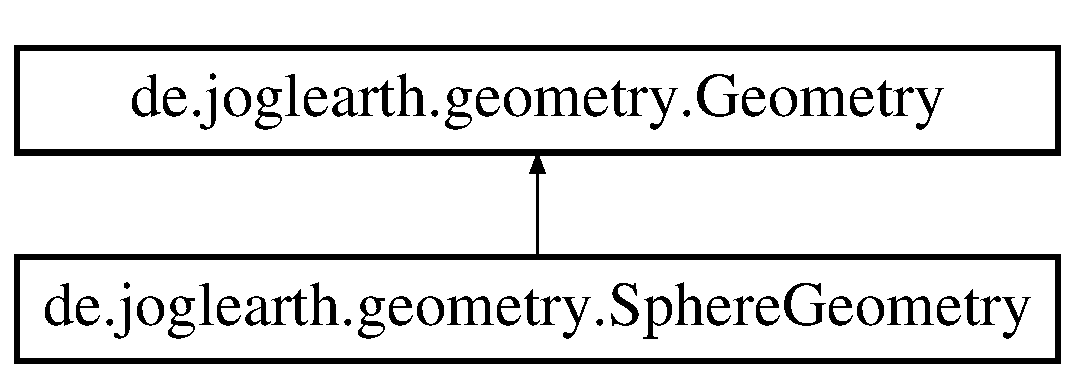
\includegraphics[height=2.000000cm]{classde_1_1joglearth_1_1geometry_1_1_sphere_geometry}
\end{center}
\end{figure}
\subsection*{Öffentliche \-Methoden}
\begin{DoxyCompactItemize}
\item 
boolean {\bf is\-Point\-Visible} ({\bf \-Geo\-Coordinates} geo)
\item 
{\bf \-Vector3} {\bf get\-Space\-Position} ({\bf \-Geo\-Coordinates} geo)
\item 
{\bf \-Screen\-Coordinates} {\bf get\-Surface\-Coordinates} ({\bf \-Vector3} view\-Vector)
\item 
{\bf \-Matrix4} {\bf get\-View\-Matrix} ()
\end{DoxyCompactItemize}


\subsection{\-Dokumentation der \-Elementfunktionen}
\index{de\-::joglearth\-::geometry\-::\-Sphere\-Geometry@{de\-::joglearth\-::geometry\-::\-Sphere\-Geometry}!get\-Space\-Position@{get\-Space\-Position}}
\index{get\-Space\-Position@{get\-Space\-Position}!de::joglearth::geometry::SphereGeometry@{de\-::joglearth\-::geometry\-::\-Sphere\-Geometry}}
\subsubsection[{get\-Space\-Position}]{\setlength{\rightskip}{0pt plus 5cm}{\bf \-Vector3} {\bf de.\-joglearth.\-geometry.\-Sphere\-Geometry.\-get\-Space\-Position} (
\begin{DoxyParamCaption}
\item[{{\bf \-Geo\-Coordinates}}]{geo}
\end{DoxyParamCaption}
)}\label{classde_1_1joglearth_1_1geometry_1_1_sphere_geometry_a058f9d046e2c3d7dd26747eec134d0a1}
\-Determines the three-\/dimensional position of a surface point in model space. \-The height map is ignored.


\begin{DoxyParams}{\-Parameter}
{\em geo} & \-The surface point. \\
\hline
\end{DoxyParams}
\begin{DoxyReturn}{\-Rückgabe}
\-The position. 
\end{DoxyReturn}


\-Implementiert {\bf de.\-joglearth.\-geometry.\-Geometry} \doxyref{}{\-S.}{interfacede_1_1joglearth_1_1geometry_1_1_geometry_a8fa1da4fcc3f99eb998a5db2f22cb2eb}.

\index{de\-::joglearth\-::geometry\-::\-Sphere\-Geometry@{de\-::joglearth\-::geometry\-::\-Sphere\-Geometry}!get\-Surface\-Coordinates@{get\-Surface\-Coordinates}}
\index{get\-Surface\-Coordinates@{get\-Surface\-Coordinates}!de::joglearth::geometry::SphereGeometry@{de\-::joglearth\-::geometry\-::\-Sphere\-Geometry}}
\subsubsection[{get\-Surface\-Coordinates}]{\setlength{\rightskip}{0pt plus 5cm}{\bf \-Screen\-Coordinates} {\bf de.\-joglearth.\-geometry.\-Sphere\-Geometry.\-get\-Surface\-Coordinates} (
\begin{DoxyParamCaption}
\item[{{\bf \-Vector3}}]{view\-Vector}
\end{DoxyParamCaption}
)}\label{classde_1_1joglearth_1_1geometry_1_1_sphere_geometry_a59b8d62f478dde615bb2794e46fb64a7}
\-Calculates the surface coordinates of the intersection from a straight line between a given point and the model center (\-The globes center or infinity for the map plane) and the map surface.


\begin{DoxyParams}{\-Parameter}
{\em view\-Vector} & \-The origin point. \\
\hline
\end{DoxyParams}
\begin{DoxyReturn}{\-Rückgabe}
\-The surface coordinates. 
\end{DoxyReturn}


\-Implementiert {\bf de.\-joglearth.\-geometry.\-Geometry} \doxyref{}{\-S.}{interfacede_1_1joglearth_1_1geometry_1_1_geometry_a65efb18a90aeacc6ba446c3cbf9f4787}.

\index{de\-::joglearth\-::geometry\-::\-Sphere\-Geometry@{de\-::joglearth\-::geometry\-::\-Sphere\-Geometry}!get\-View\-Matrix@{get\-View\-Matrix}}
\index{get\-View\-Matrix@{get\-View\-Matrix}!de::joglearth::geometry::SphereGeometry@{de\-::joglearth\-::geometry\-::\-Sphere\-Geometry}}
\subsubsection[{get\-View\-Matrix}]{\setlength{\rightskip}{0pt plus 5cm}{\bf \-Matrix4} {\bf de.\-joglearth.\-geometry.\-Sphere\-Geometry.\-get\-View\-Matrix} (
\begin{DoxyParamCaption}
{}
\end{DoxyParamCaption}
)}\label{classde_1_1joglearth_1_1geometry_1_1_sphere_geometry_adaebcd9cc9c9e5c6146dd699c701cdba}
\-Returns the view matrix performing translations and rotations incurred by the camera position.

\begin{DoxyReturn}{\-Rückgabe}
\-The view matrix. 
\end{DoxyReturn}


\-Implementiert {\bf de.\-joglearth.\-geometry.\-Geometry} \doxyref{}{\-S.}{interfacede_1_1joglearth_1_1geometry_1_1_geometry_a30f45d30257e8fc7e9d6f91cf846cdda}.

\index{de\-::joglearth\-::geometry\-::\-Sphere\-Geometry@{de\-::joglearth\-::geometry\-::\-Sphere\-Geometry}!is\-Point\-Visible@{is\-Point\-Visible}}
\index{is\-Point\-Visible@{is\-Point\-Visible}!de::joglearth::geometry::SphereGeometry@{de\-::joglearth\-::geometry\-::\-Sphere\-Geometry}}
\subsubsection[{is\-Point\-Visible}]{\setlength{\rightskip}{0pt plus 5cm}boolean {\bf de.\-joglearth.\-geometry.\-Sphere\-Geometry.\-is\-Point\-Visible} (
\begin{DoxyParamCaption}
\item[{{\bf \-Geo\-Coordinates}}]{geo}
\end{DoxyParamCaption}
)}\label{classde_1_1joglearth_1_1geometry_1_1_sphere_geometry_a224b024410063b95a3ec51fcc983effb}
\-Returns whether a point, given by longitude and latitude coordinates, could be visible given that the field of view and distance is large enough.


\begin{DoxyParams}{\-Parameter}
{\em geo} & \-The surface point. \\
\hline
\end{DoxyParams}
\begin{DoxyReturn}{\-Rückgabe}
\-Whether the point might be visible. 
\end{DoxyReturn}


\-Implementiert {\bf de.\-joglearth.\-geometry.\-Geometry} \doxyref{}{\-S.}{interfacede_1_1joglearth_1_1geometry_1_1_geometry_a1bca475164a399431f9f6238dd292b6a}.


\section{de.\-joglearth.\-rendering.\-Sphere\-Tessellator Klassenreferenz}
\label{classde_1_1joglearth_1_1rendering_1_1_sphere_tessellator}\index{de.\-joglearth.\-rendering.\-Sphere\-Tessellator@{de.\-joglearth.\-rendering.\-Sphere\-Tessellator}}
Klassendiagramm für de.\-joglearth.\-rendering.\-Sphere\-Tessellator\-:\begin{figure}[H]
\begin{center}
\leavevmode
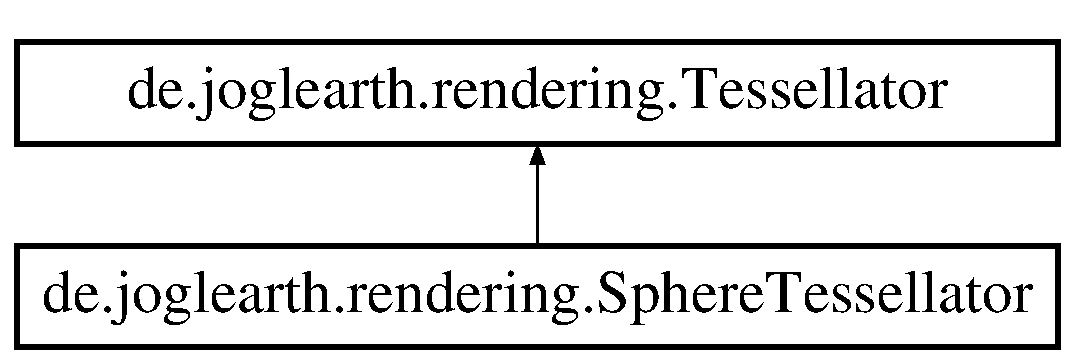
\includegraphics[height=2.000000cm]{classde_1_1joglearth_1_1rendering_1_1_sphere_tessellator}
\end{center}
\end{figure}
\subsection*{Öffentliche Methoden}
\begin{DoxyCompactItemize}
\item 
{\bf Mesh} {\bf tessellate\-Tile} ({\bf Tile} tile, int subdivisions, boolean height\-Map)
\end{DoxyCompactItemize}


\subsection{Ausführliche Beschreibung}
Generates \doxyref{Mesh}{S.}{classde_1_1joglearth_1_1rendering_1_1_mesh}es for tiles on the globe. 

\subsection{Dokumentation der Elementfunktionen}
\index{de\-::joglearth\-::rendering\-::\-Sphere\-Tessellator@{de\-::joglearth\-::rendering\-::\-Sphere\-Tessellator}!tessellate\-Tile@{tessellate\-Tile}}
\index{tessellate\-Tile@{tessellate\-Tile}!de::joglearth::rendering::SphereTessellator@{de\-::joglearth\-::rendering\-::\-Sphere\-Tessellator}}
\subsubsection[{tessellate\-Tile}]{\setlength{\rightskip}{0pt plus 5cm}{\bf Mesh} de.\-joglearth.\-rendering.\-Sphere\-Tessellator.\-tessellate\-Tile (
\begin{DoxyParamCaption}
\item[{{\bf Tile}}]{tile, }
\item[{int}]{subdivisions, }
\item[{boolean}]{height\-Map}
\end{DoxyParamCaption}
)}\label{classde_1_1joglearth_1_1rendering_1_1_sphere_tessellator_a2231f3dbde16ae862c5865fa3ddf253a}
Creates a \doxyref{Mesh}{S.}{classde_1_1joglearth_1_1rendering_1_1_mesh} for a  Tile with height data.


\begin{DoxyParams}{Parameter}
{\em tile} & The location where the {\ttfamily \doxyref{Mesh}{S.}{classde_1_1joglearth_1_1rendering_1_1_mesh}} should be rendered. \\
\hline
{\em subdivisions} & Number of times the {\ttfamily \doxyref{Mesh}{S.}{classde_1_1joglearth_1_1rendering_1_1_mesh}} is divided in both axis. Minimum {\ttfamily 0} divisions. \\
\hline
{\em height\-Map} & A \doxyref{de.\-joglearth.\-surface.\-Height\-Map}{S.}{classde_1_1joglearth_1_1surface_1_1_height_map} that provides the height data for the tile. \\
\hline
\end{DoxyParams}
\begin{DoxyReturn}{Rückgabe}
A {\ttfamily \doxyref{Mesh}{S.}{classde_1_1joglearth_1_1rendering_1_1_mesh}} with (subdivisions + 1)$^\wedge$2 squares, with each divided in two triangles. 
\end{DoxyReturn}


Implementiert {\bf de.\-joglearth.\-rendering.\-Tessellator} \doxyref{}{S.}{interfacede_1_1joglearth_1_1rendering_1_1_tessellator_a05a3cd23966d23fb0460f339aea496f0}.


\section{de.\-joglearth.\-source.\-srtm.\-S\-R\-T\-M\-Binary\-Source Klassenreferenz}
\label{classde_1_1joglearth_1_1source_1_1srtm_1_1_s_r_t_m_binary_source}\index{de.\-joglearth.\-source.\-srtm.\-S\-R\-T\-M\-Binary\-Source@{de.\-joglearth.\-source.\-srtm.\-S\-R\-T\-M\-Binary\-Source}}
Klassendiagramm für de.\-joglearth.\-source.\-srtm.\-S\-R\-T\-M\-Binary\-Source\-:\begin{figure}[H]
\begin{center}
\leavevmode
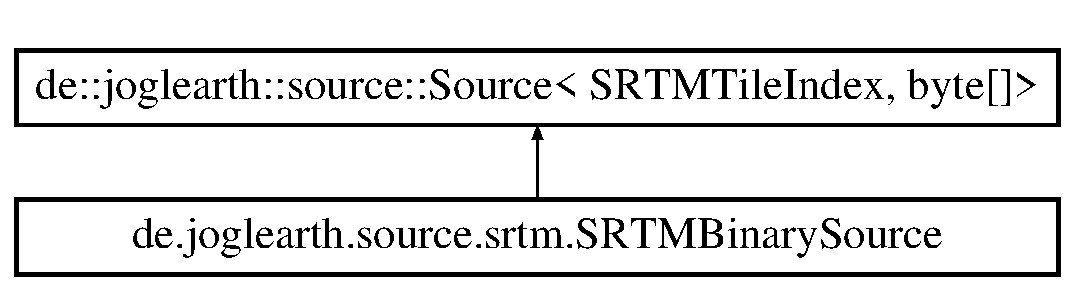
\includegraphics[height=2.000000cm]{classde_1_1joglearth_1_1source_1_1srtm_1_1_s_r_t_m_binary_source}
\end{center}
\end{figure}
\subsection*{Öffentliche Methoden}
\begin{DoxyCompactItemize}
\item 
{\bf S\-R\-T\-M\-Binary\-Source} ()
\item 
Source\-Response$<$ byte[$\,$]$>$ {\bfseries request\-Object} ({\bf S\-R\-T\-M\-Tile\-Index} key, Source\-Listener$<$ {\bf S\-R\-T\-M\-Tile\-Index}, byte[$\,$]$>$ sender)\label{classde_1_1joglearth_1_1source_1_1srtm_1_1_s_r_t_m_binary_source_ad64fc64f0d6adbd265a4dd15a9bf4c40}

\end{DoxyCompactItemize}


\subsection{Ausführliche Beschreibung}
Uses the \doxyref{H\-T\-T\-P}{S.}{} to get the S\-R\-T\-M data from N\-A\-S\-A servers. The size of the S\-R\-T\-M tiles is 90 x 90 meters. The S\-R\-T\-M tiles include all information of a required point about the height above the sea level. Only necessary if the Hight\-Profile is activated. 

\subsection{Beschreibung der Konstruktoren und Destruktoren}
\index{de\-::joglearth\-::source\-::srtm\-::\-S\-R\-T\-M\-Binary\-Source@{de\-::joglearth\-::source\-::srtm\-::\-S\-R\-T\-M\-Binary\-Source}!S\-R\-T\-M\-Binary\-Source@{S\-R\-T\-M\-Binary\-Source}}
\index{S\-R\-T\-M\-Binary\-Source@{S\-R\-T\-M\-Binary\-Source}!de::joglearth::source::srtm::SRTMBinarySource@{de\-::joglearth\-::source\-::srtm\-::\-S\-R\-T\-M\-Binary\-Source}}
\subsubsection[{S\-R\-T\-M\-Binary\-Source}]{\setlength{\rightskip}{0pt plus 5cm}de.\-joglearth.\-source.\-srtm.\-S\-R\-T\-M\-Binary\-Source.\-S\-R\-T\-M\-Binary\-Source (
\begin{DoxyParamCaption}
{}
\end{DoxyParamCaption}
)}\label{classde_1_1joglearth_1_1source_1_1srtm_1_1_s_r_t_m_binary_source_aa0da344b6f87942fdebd57d0139e5509}
Constructor. Initializes the \doxyref{S\-R\-T\-M\-Tile\-Source}{S.}{classde_1_1joglearth_1_1source_1_1srtm_1_1_s_r_t_m_tile_source}.


\begin{DoxyParams}{Parameter}
{\em servers} & An array of servers delivered as Strings \\
\hline
\end{DoxyParams}

\section{de.\-joglearth.\-source.\-srtm.\-S\-R\-T\-M\-Path\-Translator Klassenreferenz}
\label{classde_1_1joglearth_1_1source_1_1srtm_1_1_s_r_t_m_path_translator}\index{de.\-joglearth.\-source.\-srtm.\-S\-R\-T\-M\-Path\-Translator@{de.\-joglearth.\-source.\-srtm.\-S\-R\-T\-M\-Path\-Translator}}


Abgeleitet von Path\-Translator$<$ S\-R\-T\-M\-Tile\-Index $>$.

\subsection*{Öffentliche Methoden}
\begin{DoxyCompactItemize}
\item 
String {\bfseries to\-File\-System\-Path} ({\bf S\-R\-T\-M\-Tile\-Index} k)\label{classde_1_1joglearth_1_1source_1_1srtm_1_1_s_r_t_m_path_translator_a76ef87db7c98e35b4cf18c3a717f8312}

\item 
{\bf S\-R\-T\-M\-Tile\-Index} {\bfseries from\-File\-System\-Path} (String s)\label{classde_1_1joglearth_1_1source_1_1srtm_1_1_s_r_t_m_path_translator_a1d8d95cecaab190368a542b713fe671b}

\end{DoxyCompactItemize}


\subsection{Ausführliche Beschreibung}
Implements the \doxyref{Path\-Translator}{S.}{} interface for S\-R\-T\-M height data tiles. 
\section{de.\-joglearth.\-source.\-srtm.\-S\-R\-T\-M\-Tile Klassenreferenz}
\label{classde_1_1joglearth_1_1source_1_1srtm_1_1_s_r_t_m_tile}\index{de.\-joglearth.\-source.\-srtm.\-S\-R\-T\-M\-Tile@{de.\-joglearth.\-source.\-srtm.\-S\-R\-T\-M\-Tile}}
\subsection*{Öffentliche Methoden}
\begin{DoxyCompactItemize}
\item 
{\bf S\-R\-T\-M\-Tile} (byte[$\,$] raw)
\item 
short[$\,$][$\,$] {\bf get\-Tile} (int lod)
\end{DoxyCompactItemize}


\subsection{Ausführliche Beschreibung}
Provides access to two-\/dimensional S\-R\-T\-M height data. 

\subsection{Beschreibung der Konstruktoren und Destruktoren}
\index{de\-::joglearth\-::source\-::srtm\-::\-S\-R\-T\-M\-Tile@{de\-::joglearth\-::source\-::srtm\-::\-S\-R\-T\-M\-Tile}!S\-R\-T\-M\-Tile@{S\-R\-T\-M\-Tile}}
\index{S\-R\-T\-M\-Tile@{S\-R\-T\-M\-Tile}!de::joglearth::source::srtm::SRTMTile@{de\-::joglearth\-::source\-::srtm\-::\-S\-R\-T\-M\-Tile}}
\subsubsection[{S\-R\-T\-M\-Tile}]{\setlength{\rightskip}{0pt plus 5cm}de.\-joglearth.\-source.\-srtm.\-S\-R\-T\-M\-Tile.\-S\-R\-T\-M\-Tile (
\begin{DoxyParamCaption}
\item[{byte[$\,$]}]{raw}
\end{DoxyParamCaption}
)}\label{classde_1_1joglearth_1_1source_1_1srtm_1_1_s_r_t_m_tile_a54261af22b3e5def1269ec5d9e42416a}
Constructor. Decodes the height information from binary S\-R\-T\-M data.


\begin{DoxyParams}{Parameter}
{\em raw} & The binary data \\
\hline
\end{DoxyParams}


\subsection{Dokumentation der Elementfunktionen}
\index{de\-::joglearth\-::source\-::srtm\-::\-S\-R\-T\-M\-Tile@{de\-::joglearth\-::source\-::srtm\-::\-S\-R\-T\-M\-Tile}!get\-Tile@{get\-Tile}}
\index{get\-Tile@{get\-Tile}!de::joglearth::source::srtm::SRTMTile@{de\-::joglearth\-::source\-::srtm\-::\-S\-R\-T\-M\-Tile}}
\subsubsection[{get\-Tile}]{\setlength{\rightskip}{0pt plus 5cm}short [$\,$][$\,$] de.\-joglearth.\-source.\-srtm.\-S\-R\-T\-M\-Tile.\-get\-Tile (
\begin{DoxyParamCaption}
\item[{int}]{lod}
\end{DoxyParamCaption}
)}\label{classde_1_1joglearth_1_1source_1_1srtm_1_1_s_r_t_m_tile_aee10576cfcf9c6001e8eaaa668736e24}
Returns a two-\/dimensional array containing the height data interpolated to 1/(4$^\wedge$lod) the size.


\begin{DoxyParams}{Parameter}
{\em lod} & The \doxyref{de.\-joglearth.\-rendering.\-Level\-Of\-Detail}{S.}{enumde_1_1joglearth_1_1rendering_1_1_level_of_detail} of the data \\
\hline
\end{DoxyParams}
\begin{DoxyReturn}{Rückgabe}
Two-\/dimensional array containing the height data 
\end{DoxyReturn}

\section{de.\-joglearth.\-source.\-srtm.\-S\-R\-T\-M\-Tile\-Index Klassenreferenz}
\label{classde_1_1joglearth_1_1source_1_1srtm_1_1_s_r_t_m_tile_index}\index{de.\-joglearth.\-source.\-srtm.\-S\-R\-T\-M\-Tile\-Index@{de.\-joglearth.\-source.\-srtm.\-S\-R\-T\-M\-Tile\-Index}}
\subsection*{Öffentliche Methoden}
\begin{DoxyCompactItemize}
\item 
{\bfseries S\-R\-T\-M\-Tile\-Index} (int lon, int lat)\label{classde_1_1joglearth_1_1source_1_1srtm_1_1_s_r_t_m_tile_index_a180a33eeceb0625e2316fed667d814e7}

\item 
int {\bfseries hash\-Code} ()\label{classde_1_1joglearth_1_1source_1_1srtm_1_1_s_r_t_m_tile_index_a7e154c052887eb7034ecd6cbbc33f397}

\item 
boolean {\bfseries equals} (Object obj)\label{classde_1_1joglearth_1_1source_1_1srtm_1_1_s_r_t_m_tile_index_a52a8ebdf041830445c73ae272543e91a}

\item 
String {\bfseries to\-String} ()\label{classde_1_1joglearth_1_1source_1_1srtm_1_1_s_r_t_m_tile_index_a4c7b4e394776d048c9a2acf68de94638}

\end{DoxyCompactItemize}

\section{de.\-joglearth.\-source.\-srtm.\-S\-R\-T\-M\-Tile\-Manager Klassenreferenz}
\label{classde_1_1joglearth_1_1source_1_1srtm_1_1_s_r_t_m_tile_manager}\index{de.\-joglearth.\-source.\-srtm.\-S\-R\-T\-M\-Tile\-Manager@{de.\-joglearth.\-source.\-srtm.\-S\-R\-T\-M\-Tile\-Manager}}


Abgeleitet von Source$<$ S\-R\-T\-M\-Tile\-Index, S\-R\-T\-M\-Tile $>$.

\subsection*{Öffentliche Methoden}
\begin{DoxyCompactItemize}
\item 
Source\-Response$<$ {\bf S\-R\-T\-M\-Tile} $>$ {\bfseries request\-Object} ({\bf S\-R\-T\-M\-Tile\-Index} key, Source\-Listener$<$ {\bf S\-R\-T\-M\-Tile\-Index}, {\bf S\-R\-T\-M\-Tile} $>$ sender)\label{classde_1_1joglearth_1_1source_1_1srtm_1_1_s_r_t_m_tile_manager_a550623a000605af3dc7527d07bc74a74}

\item 
void {\bf add\-Surface\-Listener} ({\bf Surface\-Listener} l)
\item 
void {\bf remove\-Surface\-Listener} ({\bf Surface\-Listener} l)
\end{DoxyCompactItemize}
\subsection*{Öffentliche, statische Methoden}
\begin{DoxyCompactItemize}
\item 
static {\bf S\-R\-T\-M\-Tile\-Manager} {\bf get\-Instance} ()
\end{DoxyCompactItemize}


\subsection{Ausführliche Beschreibung}
Singleton class that retrieves data from the \doxyref{S\-R\-T\-M\-Tile\-Source}{S.}{classde_1_1joglearth_1_1source_1_1srtm_1_1_s_r_t_m_tile_source}. 

\subsection{Dokumentation der Elementfunktionen}
\index{de\-::joglearth\-::source\-::srtm\-::\-S\-R\-T\-M\-Tile\-Manager@{de\-::joglearth\-::source\-::srtm\-::\-S\-R\-T\-M\-Tile\-Manager}!add\-Surface\-Listener@{add\-Surface\-Listener}}
\index{add\-Surface\-Listener@{add\-Surface\-Listener}!de::joglearth::source::srtm::SRTMTileManager@{de\-::joglearth\-::source\-::srtm\-::\-S\-R\-T\-M\-Tile\-Manager}}
\subsubsection[{add\-Surface\-Listener}]{\setlength{\rightskip}{0pt plus 5cm}void de.\-joglearth.\-source.\-srtm.\-S\-R\-T\-M\-Tile\-Manager.\-add\-Surface\-Listener (
\begin{DoxyParamCaption}
\item[{{\bf Surface\-Listener}}]{l}
\end{DoxyParamCaption}
)}\label{classde_1_1joglearth_1_1source_1_1srtm_1_1_s_r_t_m_tile_manager_a89be1c30bb09cd331cb178832cbb65b3}
Adds a new \doxyref{Surface\-Listener}{S.}{}.


\begin{DoxyParams}{Parameter}
{\em l} & The new \doxyref{Surface\-Listener}{S.}{} \\
\hline
\end{DoxyParams}
\index{de\-::joglearth\-::source\-::srtm\-::\-S\-R\-T\-M\-Tile\-Manager@{de\-::joglearth\-::source\-::srtm\-::\-S\-R\-T\-M\-Tile\-Manager}!get\-Instance@{get\-Instance}}
\index{get\-Instance@{get\-Instance}!de::joglearth::source::srtm::SRTMTileManager@{de\-::joglearth\-::source\-::srtm\-::\-S\-R\-T\-M\-Tile\-Manager}}
\subsubsection[{get\-Instance}]{\setlength{\rightskip}{0pt plus 5cm}static {\bf S\-R\-T\-M\-Tile\-Manager} de.\-joglearth.\-source.\-srtm.\-S\-R\-T\-M\-Tile\-Manager.\-get\-Instance (
\begin{DoxyParamCaption}
{}
\end{DoxyParamCaption}
)\hspace{0.3cm}{\ttfamily [static]}}\label{classde_1_1joglearth_1_1source_1_1srtm_1_1_s_r_t_m_tile_manager_a35779b3791c0b99d85cbf28e7f9a3edd}
Returns the instance of the class or creates it, if it does not exist yet.

\begin{DoxyReturn}{Rückgabe}
The instance of \doxyref{S\-R\-T\-M\-Tile\-Manager}{S.}{classde_1_1joglearth_1_1source_1_1srtm_1_1_s_r_t_m_tile_manager} 
\end{DoxyReturn}
\index{de\-::joglearth\-::source\-::srtm\-::\-S\-R\-T\-M\-Tile\-Manager@{de\-::joglearth\-::source\-::srtm\-::\-S\-R\-T\-M\-Tile\-Manager}!remove\-Surface\-Listener@{remove\-Surface\-Listener}}
\index{remove\-Surface\-Listener@{remove\-Surface\-Listener}!de::joglearth::source::srtm::SRTMTileManager@{de\-::joglearth\-::source\-::srtm\-::\-S\-R\-T\-M\-Tile\-Manager}}
\subsubsection[{remove\-Surface\-Listener}]{\setlength{\rightskip}{0pt plus 5cm}void de.\-joglearth.\-source.\-srtm.\-S\-R\-T\-M\-Tile\-Manager.\-remove\-Surface\-Listener (
\begin{DoxyParamCaption}
\item[{{\bf Surface\-Listener}}]{l}
\end{DoxyParamCaption}
)}\label{classde_1_1joglearth_1_1source_1_1srtm_1_1_s_r_t_m_tile_manager_a669c41f02243b7fe3fba9e8176488b67}
Removes a given \doxyref{Surface\-Listener}{S.}{}.


\begin{DoxyParams}{Parameter}
{\em l} & The \doxyref{Surface\-Listener}{S.}{} that should be removed \\
\hline
\end{DoxyParams}

\section{de.\-joglearth.\-source.\-srtm.\-S\-R\-T\-M\-Tile\-Source Klassenreferenz}
\label{classde_1_1joglearth_1_1source_1_1srtm_1_1_s_r_t_m_tile_source}\index{de.\-joglearth.\-source.\-srtm.\-S\-R\-T\-M\-Tile\-Source@{de.\-joglearth.\-source.\-srtm.\-S\-R\-T\-M\-Tile\-Source}}


Abgeleitet von Source$<$ S\-R\-T\-M\-Tile\-Index, S\-R\-T\-M\-Tile $>$.

\subsection*{Öffentliche Methoden}
\begin{DoxyCompactItemize}
\item 
{\bf S\-R\-T\-M\-Tile\-Source} (Source$<$ {\bf S\-R\-T\-M\-Tile\-Index}, byte[$\,$]$>$ binary\-Source)
\item 
Source\-Response$<$ {\bf S\-R\-T\-M\-Tile} $>$ {\bfseries request\-Object} ({\bf S\-R\-T\-M\-Tile\-Index} k, Source\-Listener$<$ {\bf S\-R\-T\-M\-Tile\-Index}, {\bf S\-R\-T\-M\-Tile} $>$ sender)\label{classde_1_1joglearth_1_1source_1_1srtm_1_1_s_r_t_m_tile_source_a0d95e07ac6234f6740f85e7ba2e1b0fc}

\end{DoxyCompactItemize}


\subsection{Ausführliche Beschreibung}
Loads S\-R\-T\-M data from N\-A\-S\-A servers. The level of detail of a pixel in the S\-R\-T\-M tiles is 90 x 90 meters. The S\-R\-T\-M tiles include all information of a required point about the height. As 'standard elevation zero' the W\-G\-S84 spheroid is used. Necessary when the Height\-Profile is activated. Only necessary if the Hight\-Profile is activated. 

\subsection{Beschreibung der Konstruktoren und Destruktoren}
\index{de\-::joglearth\-::source\-::srtm\-::\-S\-R\-T\-M\-Tile\-Source@{de\-::joglearth\-::source\-::srtm\-::\-S\-R\-T\-M\-Tile\-Source}!S\-R\-T\-M\-Tile\-Source@{S\-R\-T\-M\-Tile\-Source}}
\index{S\-R\-T\-M\-Tile\-Source@{S\-R\-T\-M\-Tile\-Source}!de::joglearth::source::srtm::SRTMTileSource@{de\-::joglearth\-::source\-::srtm\-::\-S\-R\-T\-M\-Tile\-Source}}
\subsubsection[{S\-R\-T\-M\-Tile\-Source}]{\setlength{\rightskip}{0pt plus 5cm}de.\-joglearth.\-source.\-srtm.\-S\-R\-T\-M\-Tile\-Source.\-S\-R\-T\-M\-Tile\-Source (
\begin{DoxyParamCaption}
\item[{Source$<$ {\bf S\-R\-T\-M\-Tile\-Index}, byte[$\,$]$>$}]{binary\-Source}
\end{DoxyParamCaption}
)}\label{classde_1_1joglearth_1_1source_1_1srtm_1_1_s_r_t_m_tile_source_a92d4e677775f995de445953de408fac5}
Constructor. Initializes the \doxyref{S\-R\-T\-M\-Tile\-Source}{S.}{classde_1_1joglearth_1_1source_1_1srtm_1_1_s_r_t_m_tile_source} as it assigns a value to the \doxyref{Source}{S.}{} of {\ttfamily \doxyref{S\-R\-T\-M\-Tile\-Source}{S.}{classde_1_1joglearth_1_1source_1_1srtm_1_1_s_r_t_m_tile_source}} 
\begin{DoxyParams}{Parameter}
{\em binary\-Source} & The {\ttfamily Source} thats assigned \\
\hline
\end{DoxyParams}

\section{de.\-joglearth.\-surface.\-Surface\-Listener Schnittstellenreferenz}
\label{interfacede_1_1joglearth_1_1surface_1_1_surface_listener}\index{de.\-joglearth.\-surface.\-Surface\-Listener@{de.\-joglearth.\-surface.\-Surface\-Listener}}


Basisklasse für de.\-joglearth.\-geometry.\-Camera.\-Surface\-Height\-Listener, de.\-joglearth.\-rendering.\-Renderer.\-Surface\-Validator und de.\-joglearth.\-ui.\-Main\-Window.\-U\-I\-Surface\-Listener.

\subsection*{Öffentliche Methoden}
\begin{DoxyCompactItemize}
\item 
void {\bf surface\-Changed} (double lon\-From, double lat\-From, double lon\-To, double lat\-To)
\end{DoxyCompactItemize}


\subsection{Ausführliche Beschreibung}
Classes implementing this interface can be notified about individual changes of displayed tiles. 

\subsection{Dokumentation der Elementfunktionen}
\index{de\-::joglearth\-::surface\-::\-Surface\-Listener@{de\-::joglearth\-::surface\-::\-Surface\-Listener}!surface\-Changed@{surface\-Changed}}
\index{surface\-Changed@{surface\-Changed}!de::joglearth::surface::SurfaceListener@{de\-::joglearth\-::surface\-::\-Surface\-Listener}}
\subsubsection[{surface\-Changed}]{\setlength{\rightskip}{0pt plus 5cm}void de.\-joglearth.\-surface.\-Surface\-Listener.\-surface\-Changed (
\begin{DoxyParamCaption}
\item[{double}]{lon\-From, }
\item[{double}]{lat\-From, }
\item[{double}]{lon\-To, }
\item[{double}]{lat\-To}
\end{DoxyParamCaption}
)}\label{interfacede_1_1joglearth_1_1surface_1_1_surface_listener_a2237442eb4673a5d6c8e859f50bce0bc}
Receives if the surface i a given area has been changed.


\begin{DoxyParams}{Parameter}
{\em tile} & A new \doxyref{Tile}{S.}{} that should be displayed now \\
\hline
\end{DoxyParams}

\section{de.\-joglearth.\-rendering.\-Tessellator Schnittstellenreferenz}
\label{interfacede_1_1joglearth_1_1rendering_1_1_tessellator}\index{de.\-joglearth.\-rendering.\-Tessellator@{de.\-joglearth.\-rendering.\-Tessellator}}
Klassendiagramm für de.\-joglearth.\-rendering.\-Tessellator\-:\begin{figure}[H]
\begin{center}
\leavevmode
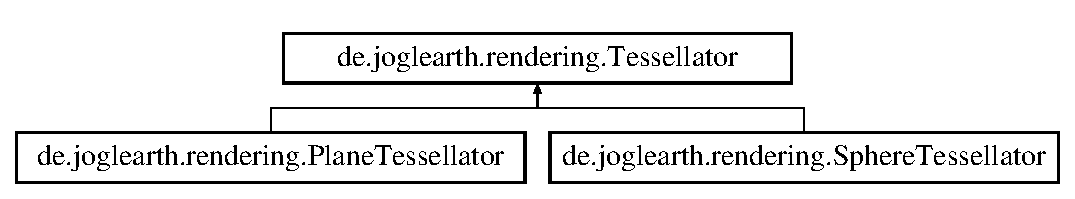
\includegraphics[height=2.000000cm]{interfacede_1_1joglearth_1_1rendering_1_1_tessellator}
\end{center}
\end{figure}
\subsection*{Öffentliche Methoden}
\begin{DoxyCompactItemize}
\item 
{\bf Mesh} {\bf tessellate\-Tile} ({\bf Tile} tile, int subdivisions, boolean height\-Map)
\end{DoxyCompactItemize}


\subsection{Ausführliche Beschreibung}
An implementation of the {\ttfamily Tesselator} Interface provides the occastion to generate a \doxyref{Mesh}{S.}{classde_1_1joglearth_1_1rendering_1_1_mesh}. 

\subsection{Dokumentation der Elementfunktionen}
\index{de\-::joglearth\-::rendering\-::\-Tessellator@{de\-::joglearth\-::rendering\-::\-Tessellator}!tessellate\-Tile@{tessellate\-Tile}}
\index{tessellate\-Tile@{tessellate\-Tile}!de::joglearth::rendering::Tessellator@{de\-::joglearth\-::rendering\-::\-Tessellator}}
\subsubsection[{tessellate\-Tile}]{\setlength{\rightskip}{0pt plus 5cm}{\bf Mesh} de.\-joglearth.\-rendering.\-Tessellator.\-tessellate\-Tile (
\begin{DoxyParamCaption}
\item[{{\bf Tile}}]{tile, }
\item[{int}]{subdivisions, }
\item[{boolean}]{height\-Map}
\end{DoxyParamCaption}
)}\label{interfacede_1_1joglearth_1_1rendering_1_1_tessellator_a05a3cd23966d23fb0460f339aea496f0}
Creates a \doxyref{Mesh}{S.}{classde_1_1joglearth_1_1rendering_1_1_mesh} for a  Tile with height data.


\begin{DoxyParams}{Parameter}
{\em tile} & The location where the {\ttfamily \doxyref{Mesh}{S.}{classde_1_1joglearth_1_1rendering_1_1_mesh}} should be rendered. \\
\hline
{\em subdivisions} & Number of times the {\ttfamily \doxyref{Mesh}{S.}{classde_1_1joglearth_1_1rendering_1_1_mesh}} is divided in both axis. Minimum {\ttfamily 0} divisions. \\
\hline
{\em height\-Map} & A \doxyref{de.\-joglearth.\-surface.\-Height\-Map}{S.}{classde_1_1joglearth_1_1surface_1_1_height_map} that provides the height data for the tile. \\
\hline
\end{DoxyParams}
\begin{DoxyReturn}{Rückgabe}
A {\ttfamily \doxyref{Mesh}{S.}{classde_1_1joglearth_1_1rendering_1_1_mesh}} with (subdivisions + 1)$^\wedge$2 squares, with each divided in two triangles. 
\end{DoxyReturn}


Implementiert in {\bf de.\-joglearth.\-rendering.\-Sphere\-Tessellator} \doxyref{}{S.}{classde_1_1joglearth_1_1rendering_1_1_sphere_tessellator_a2231f3dbde16ae862c5865fa3ddf253a} und {\bf de.\-joglearth.\-rendering.\-Plane\-Tessellator} \doxyref{}{S.}{classde_1_1joglearth_1_1rendering_1_1_plane_tessellator_a18c9e45cfb94086cb93e1f10076414cc}.


\section{de.\-joglearth.\-source.\-opengl.\-Texture\-Cache Klassenreferenz}
\label{classde_1_1joglearth_1_1source_1_1opengl_1_1_texture_cache}\index{de.\-joglearth.\-source.\-opengl.\-Texture\-Cache@{de.\-joglearth.\-source.\-opengl.\-Texture\-Cache}}
Klassendiagramm für de.\-joglearth.\-source.\-opengl.\-Texture\-Cache\-:\begin{figure}[H]
\begin{center}
\leavevmode
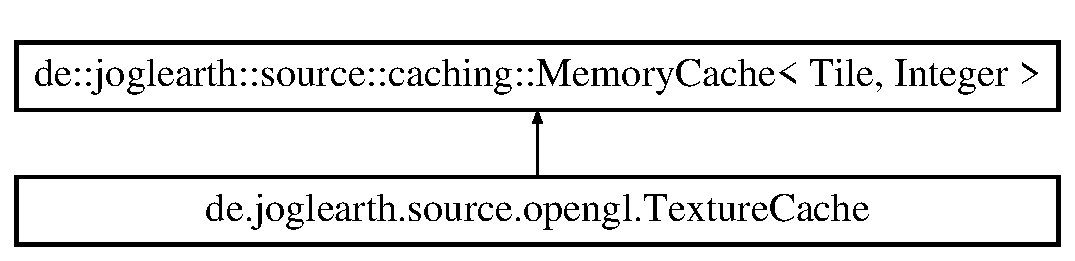
\includegraphics[height=2.000000cm]{classde_1_1joglearth_1_1source_1_1opengl_1_1_texture_cache}
\end{center}
\end{figure}
\subsection*{Öffentliche Methoden}
\begin{DoxyCompactItemize}
\item 
void {\bfseries drop\-Object} ({\bf Tile} k)\label{classde_1_1joglearth_1_1source_1_1opengl_1_1_texture_cache_af78af343a17ade633613f278d1e16c26}

\end{DoxyCompactItemize}


\subsection{Ausführliche Beschreibung}
Manages and displaces textures in Open\-Gl graphics memory. 
\section{de.\-joglearth.\-surface.\-Texture\-Manager Klassenreferenz}
\label{classde_1_1joglearth_1_1surface_1_1_texture_manager}\index{de.\-joglearth.\-surface.\-Texture\-Manager@{de.\-joglearth.\-surface.\-Texture\-Manager}}
\subsection*{Öffentliche Methoden}
\begin{DoxyCompactItemize}
\item 
{\bfseries Texture\-Manager} (G\-L2 gl)\label{classde_1_1joglearth_1_1surface_1_1_texture_manager_ab4a96d2d19cd167c7875f9d6002f1237}

\item 
Integer {\bf get\-Texture} ({\bf Tile} tile)
\item 
void {\bf add\-Surface\-Listener} ({\bf Surface\-Listener} l)
\item 
void {\bf remove\-Surface\-Listener} ({\bf Surface\-Listener} l)
\end{DoxyCompactItemize}


\subsection{Ausführliche Beschreibung}
Executes requests for textures of the \doxyref{Renderer}{S.}{}. Loads textures from a \doxyref{Request\-Distrubutor}{S.}{} which accesses a \doxyref{Tile\-Texture\-Source}{S.}{} and a \doxyref{Texture\-Cache}{S.}{}. 

\subsection{Dokumentation der Elementfunktionen}
\index{de\-::joglearth\-::surface\-::\-Texture\-Manager@{de\-::joglearth\-::surface\-::\-Texture\-Manager}!add\-Surface\-Listener@{add\-Surface\-Listener}}
\index{add\-Surface\-Listener@{add\-Surface\-Listener}!de::joglearth::surface::TextureManager@{de\-::joglearth\-::surface\-::\-Texture\-Manager}}
\subsubsection[{add\-Surface\-Listener}]{\setlength{\rightskip}{0pt plus 5cm}void de.\-joglearth.\-surface.\-Texture\-Manager.\-add\-Surface\-Listener (
\begin{DoxyParamCaption}
\item[{{\bf Surface\-Listener}}]{l}
\end{DoxyParamCaption}
)}\label{classde_1_1joglearth_1_1surface_1_1_texture_manager_afb2aebc58c0a2f978a6be6cd9519ef3e}
Adds a \doxyref{Surface\-Listener}{S.}{interfacede_1_1joglearth_1_1surface_1_1_surface_listener} that distributes a notification if the surface was changed.


\begin{DoxyParams}{Parameter}
{\em l} & The new listener \\
\hline
\end{DoxyParams}
\index{de\-::joglearth\-::surface\-::\-Texture\-Manager@{de\-::joglearth\-::surface\-::\-Texture\-Manager}!get\-Texture@{get\-Texture}}
\index{get\-Texture@{get\-Texture}!de::joglearth::surface::TextureManager@{de\-::joglearth\-::surface\-::\-Texture\-Manager}}
\subsubsection[{get\-Texture}]{\setlength{\rightskip}{0pt plus 5cm}Integer de.\-joglearth.\-surface.\-Texture\-Manager.\-get\-Texture (
\begin{DoxyParamCaption}
\item[{{\bf Tile}}]{tile}
\end{DoxyParamCaption}
)}\label{classde_1_1joglearth_1_1surface_1_1_texture_manager_a43db8e62afce691ad798599d61ff034a}
Is called if a texture of a \doxyref{Tile}{S.}{} should be loaded.


\begin{DoxyParams}{Parameter}
{\em tile} & The \doxyref{Tile}{S.}{} that should be loaded \\
\hline
\end{DoxyParams}
\begin{DoxyReturn}{Rückgabe}
Returns a loaded Open\-Gl identifier for the texture or if it is not yet loaded, the method returns a place holder texture 
\end{DoxyReturn}
\index{de\-::joglearth\-::surface\-::\-Texture\-Manager@{de\-::joglearth\-::surface\-::\-Texture\-Manager}!remove\-Surface\-Listener@{remove\-Surface\-Listener}}
\index{remove\-Surface\-Listener@{remove\-Surface\-Listener}!de::joglearth::surface::TextureManager@{de\-::joglearth\-::surface\-::\-Texture\-Manager}}
\subsubsection[{remove\-Surface\-Listener}]{\setlength{\rightskip}{0pt plus 5cm}void de.\-joglearth.\-surface.\-Texture\-Manager.\-remove\-Surface\-Listener (
\begin{DoxyParamCaption}
\item[{{\bf Surface\-Listener}}]{l}
\end{DoxyParamCaption}
)}\label{classde_1_1joglearth_1_1surface_1_1_texture_manager_a71b7f9629795c6cea7c2a22750d40c34}
Removes a specific \doxyref{Surface\-Listener}{S.}{interfacede_1_1joglearth_1_1surface_1_1_surface_listener}.


\begin{DoxyParams}{Parameter}
{\em l} & The listener that should be removed \\
\hline
\end{DoxyParams}

\section{de.\-joglearth.\-geometry.\-Tile Klassenreferenz}
\label{classde_1_1joglearth_1_1geometry_1_1_tile}\index{de.\-joglearth.\-geometry.\-Tile@{de.\-joglearth.\-geometry.\-Tile}}
\subsection*{Öffentliche Methoden}
\begin{DoxyCompactItemize}
\item 
{\bf Tile} (int detail\-Level, int lon\-Index, int lat\-Index)
\item 
double {\bf longitude\-From} ()
\item 
double {\bf longitude\-To} ()
\item 
double {\bf latitude\-From} ()
\item 
double {\bf latitude\-To} ()
\item 
int {\bf get\-Longitude\-Index} ()
\item 
int {\bf get\-Latitude\-Index} ()
\item 
int {\bf get\-Detail\-Level} ()
\item 
boolean {\bfseries intersects} (double lon\-From, double lat\-From, double lon\-To, double lat\-To)\label{classde_1_1joglearth_1_1geometry_1_1_tile_adfc74c03a286841a64ce0ee042c14434}

\item 
int {\bfseries hash\-Code} ()\label{classde_1_1joglearth_1_1geometry_1_1_tile_a3b21cc339782d60f6063a2400d404818}

\item 
boolean {\bfseries equals} (Object obj)\label{classde_1_1joglearth_1_1geometry_1_1_tile_a3fe21b8a7de2e649e281ad00e97bacaf}

\item 
boolean {\bfseries contains} ({\bf Geo\-Coordinates} coords)\label{classde_1_1joglearth_1_1geometry_1_1_tile_a4f74853fb1566ecc598bdde775b0b691}

\end{DoxyCompactItemize}
\subsection*{Öffentliche, statische Methoden}
\begin{DoxyCompactItemize}
\item 
static {\bf Tile} {\bf get\-Containing\-Tile} (int detail\-Level, {\bf Geo\-Coordinates} coords)
\end{DoxyCompactItemize}


\subsection{Ausführliche Beschreibung}
A structure identifying a single Open\-Street\-Map surface tile. 

\subsection{Beschreibung der Konstruktoren und Destruktoren}
\index{de\-::joglearth\-::geometry\-::\-Tile@{de\-::joglearth\-::geometry\-::\-Tile}!Tile@{Tile}}
\index{Tile@{Tile}!de::joglearth::geometry::Tile@{de\-::joglearth\-::geometry\-::\-Tile}}
\subsubsection[{Tile}]{\setlength{\rightskip}{0pt plus 5cm}de.\-joglearth.\-geometry.\-Tile.\-Tile (
\begin{DoxyParamCaption}
\item[{int}]{detail\-Level, }
\item[{int}]{lon\-Index, }
\item[{int}]{lat\-Index}
\end{DoxyParamCaption}
)}\label{classde_1_1joglearth_1_1geometry_1_1_tile_a21a60bac9d5ded3d81bd47860f19fe3c}
Constructor.


\begin{DoxyParams}{Parameter}
{\em detail\-Level} & How often the globe is subdivided to reach the desired tile size. \\
\hline
{\em lon\-Index} & The number of tiles to skip, starting from latitude 0, to reach the left bound of the tile. \\
\hline
{\em lon\-Index} & The number of tiles to skip, starting from the north pole, to reach the desired longitude. \\
\hline
\end{DoxyParams}


\subsection{Dokumentation der Elementfunktionen}
\index{de\-::joglearth\-::geometry\-::\-Tile@{de\-::joglearth\-::geometry\-::\-Tile}!get\-Containing\-Tile@{get\-Containing\-Tile}}
\index{get\-Containing\-Tile@{get\-Containing\-Tile}!de::joglearth::geometry::Tile@{de\-::joglearth\-::geometry\-::\-Tile}}
\subsubsection[{get\-Containing\-Tile}]{\setlength{\rightskip}{0pt plus 5cm}static {\bf Tile} de.\-joglearth.\-geometry.\-Tile.\-get\-Containing\-Tile (
\begin{DoxyParamCaption}
\item[{int}]{detail\-Level, }
\item[{{\bf Geo\-Coordinates}}]{coords}
\end{DoxyParamCaption}
)\hspace{0.3cm}{\ttfamily [static]}}\label{classde_1_1joglearth_1_1geometry_1_1_tile_a007c0b6c58f25ceb56fdb3d8a9c958d0}
Returns a tile in the given detail level which contains a specific point.


\begin{DoxyParams}{Parameter}
{\em detail\-Level} & The detail level. \\
\hline
{\em coords} & The point. \\
\hline
\end{DoxyParams}
\begin{DoxyReturn}{Rückgabe}
A tile. 
\end{DoxyReturn}
\index{de\-::joglearth\-::geometry\-::\-Tile@{de\-::joglearth\-::geometry\-::\-Tile}!get\-Detail\-Level@{get\-Detail\-Level}}
\index{get\-Detail\-Level@{get\-Detail\-Level}!de::joglearth::geometry::Tile@{de\-::joglearth\-::geometry\-::\-Tile}}
\subsubsection[{get\-Detail\-Level}]{\setlength{\rightskip}{0pt plus 5cm}int de.\-joglearth.\-geometry.\-Tile.\-get\-Detail\-Level (
\begin{DoxyParamCaption}
{}
\end{DoxyParamCaption}
)}\label{classde_1_1joglearth_1_1geometry_1_1_tile_aeee190fcc6ddae39b8555f69e1eec0ec}
The detail level, as supplied in the constructor.

\begin{DoxyReturn}{Rückgabe}
The detail level. 
\end{DoxyReturn}
\index{de\-::joglearth\-::geometry\-::\-Tile@{de\-::joglearth\-::geometry\-::\-Tile}!get\-Latitude\-Index@{get\-Latitude\-Index}}
\index{get\-Latitude\-Index@{get\-Latitude\-Index}!de::joglearth::geometry::Tile@{de\-::joglearth\-::geometry\-::\-Tile}}
\subsubsection[{get\-Latitude\-Index}]{\setlength{\rightskip}{0pt plus 5cm}int de.\-joglearth.\-geometry.\-Tile.\-get\-Latitude\-Index (
\begin{DoxyParamCaption}
{}
\end{DoxyParamCaption}
)}\label{classde_1_1joglearth_1_1geometry_1_1_tile_ac792557c974806e10fed0241a9bf4732}
The latitude index, as supplied in the constructor.

\begin{DoxyReturn}{Rückgabe}
The latitude index. 
\end{DoxyReturn}
\index{de\-::joglearth\-::geometry\-::\-Tile@{de\-::joglearth\-::geometry\-::\-Tile}!get\-Longitude\-Index@{get\-Longitude\-Index}}
\index{get\-Longitude\-Index@{get\-Longitude\-Index}!de::joglearth::geometry::Tile@{de\-::joglearth\-::geometry\-::\-Tile}}
\subsubsection[{get\-Longitude\-Index}]{\setlength{\rightskip}{0pt plus 5cm}int de.\-joglearth.\-geometry.\-Tile.\-get\-Longitude\-Index (
\begin{DoxyParamCaption}
{}
\end{DoxyParamCaption}
)}\label{classde_1_1joglearth_1_1geometry_1_1_tile_ac956f26b82f9442f6f45bf59d8837d31}
The longitude index, as supplied in the constructor.

\begin{DoxyReturn}{Rückgabe}
The longitude index. 
\end{DoxyReturn}
\index{de\-::joglearth\-::geometry\-::\-Tile@{de\-::joglearth\-::geometry\-::\-Tile}!latitude\-From@{latitude\-From}}
\index{latitude\-From@{latitude\-From}!de::joglearth::geometry::Tile@{de\-::joglearth\-::geometry\-::\-Tile}}
\subsubsection[{latitude\-From}]{\setlength{\rightskip}{0pt plus 5cm}double de.\-joglearth.\-geometry.\-Tile.\-latitude\-From (
\begin{DoxyParamCaption}
{}
\end{DoxyParamCaption}
)}\label{classde_1_1joglearth_1_1geometry_1_1_tile_acbbeabff9822525bfa3e5278e3ebcfca}
Returns the lower latitude bound of the tile.

\begin{DoxyReturn}{Rückgabe}
The latitude, in radians. 
\end{DoxyReturn}
\index{de\-::joglearth\-::geometry\-::\-Tile@{de\-::joglearth\-::geometry\-::\-Tile}!latitude\-To@{latitude\-To}}
\index{latitude\-To@{latitude\-To}!de::joglearth::geometry::Tile@{de\-::joglearth\-::geometry\-::\-Tile}}
\subsubsection[{latitude\-To}]{\setlength{\rightskip}{0pt plus 5cm}double de.\-joglearth.\-geometry.\-Tile.\-latitude\-To (
\begin{DoxyParamCaption}
{}
\end{DoxyParamCaption}
)}\label{classde_1_1joglearth_1_1geometry_1_1_tile_a27333fed7739d77dca7a71cc803c07aa}
Returns the upper latitude bound of the tile.

\begin{DoxyReturn}{Rückgabe}
The latitude, in radians. 
\end{DoxyReturn}
\index{de\-::joglearth\-::geometry\-::\-Tile@{de\-::joglearth\-::geometry\-::\-Tile}!longitude\-From@{longitude\-From}}
\index{longitude\-From@{longitude\-From}!de::joglearth::geometry::Tile@{de\-::joglearth\-::geometry\-::\-Tile}}
\subsubsection[{longitude\-From}]{\setlength{\rightskip}{0pt plus 5cm}double de.\-joglearth.\-geometry.\-Tile.\-longitude\-From (
\begin{DoxyParamCaption}
{}
\end{DoxyParamCaption}
)}\label{classde_1_1joglearth_1_1geometry_1_1_tile_aeae6d2aecc73f4873e9265b0b1556ba1}
Returns the lower longitude bound of the tile.

\begin{DoxyReturn}{Rückgabe}
The longitude, in radians. 
\end{DoxyReturn}
\index{de\-::joglearth\-::geometry\-::\-Tile@{de\-::joglearth\-::geometry\-::\-Tile}!longitude\-To@{longitude\-To}}
\index{longitude\-To@{longitude\-To}!de::joglearth::geometry::Tile@{de\-::joglearth\-::geometry\-::\-Tile}}
\subsubsection[{longitude\-To}]{\setlength{\rightskip}{0pt plus 5cm}double de.\-joglearth.\-geometry.\-Tile.\-longitude\-To (
\begin{DoxyParamCaption}
{}
\end{DoxyParamCaption}
)}\label{classde_1_1joglearth_1_1geometry_1_1_tile_aca96311174354537b0d9e1774dcc1894}
Returns the upper longitude bound of the tile.

\begin{DoxyReturn}{Rückgabe}
The longitude, in radians. 
\end{DoxyReturn}

\section{de.\-joglearth.\-surface.\-Tiled\-Map\-Type Enum-\/\-Referenz}
\label{enumde_1_1joglearth_1_1surface_1_1_tiled_map_type}\index{de.\-joglearth.\-surface.\-Tiled\-Map\-Type@{de.\-joglearth.\-surface.\-Tiled\-Map\-Type}}
\subsection*{Öffentliche Attribute}
\begin{DoxyCompactItemize}
\item 
{\bf O\-S\-M\-\_\-\-M\-A\-P}
\item 
{\bf T\-R\-E\-K\-K\-I\-N\-G\-\_\-\-M\-A\-P}
\item 
{\bf S\-E\-A\-\_\-\-M\-A\-P}
\item 
{\bf C\-Y\-C\-L\-E\-\_\-\-M\-A\-P}
\item 
{\bf S\-K\-I\-\_\-\-R\-U\-N\-\_\-\-M\-A\-P}
\end{DoxyCompactItemize}


\subsection{Ausführliche Beschreibung}
Type of an Open\-Street\-Map tile. O\-S\-M tiles has a maximum zoom level of '18'. 

\subsection{Dokumentation der Datenelemente}
\index{de\-::joglearth\-::surface\-::\-Tiled\-Map\-Type@{de\-::joglearth\-::surface\-::\-Tiled\-Map\-Type}!C\-Y\-C\-L\-E\-\_\-\-M\-A\-P@{C\-Y\-C\-L\-E\-\_\-\-M\-A\-P}}
\index{C\-Y\-C\-L\-E\-\_\-\-M\-A\-P@{C\-Y\-C\-L\-E\-\_\-\-M\-A\-P}!de::joglearth::surface::TiledMapType@{de\-::joglearth\-::surface\-::\-Tiled\-Map\-Type}}
\subsubsection[{C\-Y\-C\-L\-E\-\_\-\-M\-A\-P}]{\setlength{\rightskip}{0pt plus 5cm}de.\-joglearth.\-surface.\-Tiled\-Map\-Type.\-C\-Y\-C\-L\-E\-\_\-\-M\-A\-P}\label{enumde_1_1joglearth_1_1surface_1_1_tiled_map_type_a39c55f770d0d95febbafcce6a7379e70}
Especially for bicyclists. \index{de\-::joglearth\-::surface\-::\-Tiled\-Map\-Type@{de\-::joglearth\-::surface\-::\-Tiled\-Map\-Type}!O\-S\-M\-\_\-\-M\-A\-P@{O\-S\-M\-\_\-\-M\-A\-P}}
\index{O\-S\-M\-\_\-\-M\-A\-P@{O\-S\-M\-\_\-\-M\-A\-P}!de::joglearth::surface::TiledMapType@{de\-::joglearth\-::surface\-::\-Tiled\-Map\-Type}}
\subsubsection[{O\-S\-M\-\_\-\-M\-A\-P}]{\setlength{\rightskip}{0pt plus 5cm}de.\-joglearth.\-surface.\-Tiled\-Map\-Type.\-O\-S\-M\-\_\-\-M\-A\-P}\label{enumde_1_1joglearth_1_1surface_1_1_tiled_map_type_a8c4d69d1979be3b0d53ef9fa11195980}
Open\-Street\-Map maps. \index{de\-::joglearth\-::surface\-::\-Tiled\-Map\-Type@{de\-::joglearth\-::surface\-::\-Tiled\-Map\-Type}!S\-E\-A\-\_\-\-M\-A\-P@{S\-E\-A\-\_\-\-M\-A\-P}}
\index{S\-E\-A\-\_\-\-M\-A\-P@{S\-E\-A\-\_\-\-M\-A\-P}!de::joglearth::surface::TiledMapType@{de\-::joglearth\-::surface\-::\-Tiled\-Map\-Type}}
\subsubsection[{S\-E\-A\-\_\-\-M\-A\-P}]{\setlength{\rightskip}{0pt plus 5cm}de.\-joglearth.\-surface.\-Tiled\-Map\-Type.\-S\-E\-A\-\_\-\-M\-A\-P}\label{enumde_1_1joglearth_1_1surface_1_1_tiled_map_type_aaea0054a112424b843897bf2df9c3f72}
Especially for seafaring. \index{de\-::joglearth\-::surface\-::\-Tiled\-Map\-Type@{de\-::joglearth\-::surface\-::\-Tiled\-Map\-Type}!S\-K\-I\-\_\-\-R\-U\-N\-\_\-\-M\-A\-P@{S\-K\-I\-\_\-\-R\-U\-N\-\_\-\-M\-A\-P}}
\index{S\-K\-I\-\_\-\-R\-U\-N\-\_\-\-M\-A\-P@{S\-K\-I\-\_\-\-R\-U\-N\-\_\-\-M\-A\-P}!de::joglearth::surface::TiledMapType@{de\-::joglearth\-::surface\-::\-Tiled\-Map\-Type}}
\subsubsection[{S\-K\-I\-\_\-\-R\-U\-N\-\_\-\-M\-A\-P}]{\setlength{\rightskip}{0pt plus 5cm}de.\-joglearth.\-surface.\-Tiled\-Map\-Type.\-S\-K\-I\-\_\-\-R\-U\-N\-\_\-\-M\-A\-P}\label{enumde_1_1joglearth_1_1surface_1_1_tiled_map_type_a1468f95d73a717edd042b5a4a83b9cf8}
Especially for winter sports enthusiasts. \index{de\-::joglearth\-::surface\-::\-Tiled\-Map\-Type@{de\-::joglearth\-::surface\-::\-Tiled\-Map\-Type}!T\-R\-E\-K\-K\-I\-N\-G\-\_\-\-M\-A\-P@{T\-R\-E\-K\-K\-I\-N\-G\-\_\-\-M\-A\-P}}
\index{T\-R\-E\-K\-K\-I\-N\-G\-\_\-\-M\-A\-P@{T\-R\-E\-K\-K\-I\-N\-G\-\_\-\-M\-A\-P}!de::joglearth::surface::TiledMapType@{de\-::joglearth\-::surface\-::\-Tiled\-Map\-Type}}
\subsubsection[{T\-R\-E\-K\-K\-I\-N\-G\-\_\-\-M\-A\-P}]{\setlength{\rightskip}{0pt plus 5cm}de.\-joglearth.\-surface.\-Tiled\-Map\-Type.\-T\-R\-E\-K\-K\-I\-N\-G\-\_\-\-M\-A\-P}\label{enumde_1_1joglearth_1_1surface_1_1_tiled_map_type_a243a0e076dfc777e453b54a25cbab5c5}
Especially for walkers and riders. 
\section{de.\-joglearth.\-surface.\-Tile\-Mesh\-Manager Klassenreferenz}
\label{classde_1_1joglearth_1_1surface_1_1_tile_mesh_manager}\index{de.\-joglearth.\-surface.\-Tile\-Mesh\-Manager@{de.\-joglearth.\-surface.\-Tile\-Mesh\-Manager}}


Abgeleitet von Source$<$ Tile, Integer $>$.

\subsection*{Öffentliche Methoden}
\begin{DoxyCompactItemize}
\item 
{\bf Tile\-Mesh\-Manager} (G\-L2 gl, {\bf Tessellator} t)
\item 
void {\bf set\-Tessellator} ({\bf Tessellator} t)
\item 
void {\bf set\-Tile\-Subdivisions} (int sub)
\item 
void {\bf enable\-Height\-Map} (boolean enable)
\item 
Source\-Response$<$ Integer $>$ {\bfseries request\-Object} ({\bf Tile} key, Source\-Listener$<$ {\bf Tile}, Integer $>$ sender)\label{classde_1_1joglearth_1_1surface_1_1_tile_mesh_manager_a3a85a95c3f769e5821d3d17bbc09fb69}

\item 
void {\bf add\-Surface\-Listener} ({\bf Surface\-Listener} l)
\item 
void {\bf remove\-Surface\-Listener} ({\bf Surface\-Listener} l)
\end{DoxyCompactItemize}


\subsection{Ausführliche Beschreibung}
Creates and cashes tile meshes as Open\-G\-L vertex buffer objects. 

\subsection{Beschreibung der Konstruktoren und Destruktoren}
\index{de\-::joglearth\-::surface\-::\-Tile\-Mesh\-Manager@{de\-::joglearth\-::surface\-::\-Tile\-Mesh\-Manager}!Tile\-Mesh\-Manager@{Tile\-Mesh\-Manager}}
\index{Tile\-Mesh\-Manager@{Tile\-Mesh\-Manager}!de::joglearth::surface::TileMeshManager@{de\-::joglearth\-::surface\-::\-Tile\-Mesh\-Manager}}
\subsubsection[{Tile\-Mesh\-Manager}]{\setlength{\rightskip}{0pt plus 5cm}de.\-joglearth.\-surface.\-Tile\-Mesh\-Manager.\-Tile\-Mesh\-Manager (
\begin{DoxyParamCaption}
\item[{G\-L2}]{gl, }
\item[{{\bf Tessellator}}]{t}
\end{DoxyParamCaption}
)}\label{classde_1_1joglearth_1_1surface_1_1_tile_mesh_manager_ab6fb3ea0ce4a88ca127c87e08c20560b}
Creates a new \doxyref{Tile\-Mesh\-Manager}{S.}{classde_1_1joglearth_1_1surface_1_1_tile_mesh_manager} as it initializes the source, the cache, sets the \doxyref{Request\-Distributor}{S.}{} and adds a surface listener from \doxyref{Height\-Map}{S.}{classde_1_1joglearth_1_1surface_1_1_height_map}.


\begin{DoxyParams}{Parameter}
{\em gl} & The G\-L context \\
\hline
{\em t} & The \doxyref{de.\-joglearth.\-rendering.\-Tessellator}{S.}{interfacede_1_1joglearth_1_1rendering_1_1_tessellator} that should be used \\
\hline
\end{DoxyParams}


\subsection{Dokumentation der Elementfunktionen}
\index{de\-::joglearth\-::surface\-::\-Tile\-Mesh\-Manager@{de\-::joglearth\-::surface\-::\-Tile\-Mesh\-Manager}!add\-Surface\-Listener@{add\-Surface\-Listener}}
\index{add\-Surface\-Listener@{add\-Surface\-Listener}!de::joglearth::surface::TileMeshManager@{de\-::joglearth\-::surface\-::\-Tile\-Mesh\-Manager}}
\subsubsection[{add\-Surface\-Listener}]{\setlength{\rightskip}{0pt plus 5cm}void de.\-joglearth.\-surface.\-Tile\-Mesh\-Manager.\-add\-Surface\-Listener (
\begin{DoxyParamCaption}
\item[{{\bf Surface\-Listener}}]{l}
\end{DoxyParamCaption}
)}\label{classde_1_1joglearth_1_1surface_1_1_tile_mesh_manager_ab93649c9e934a0ae470dd8abdbd72cb5}
Adds a \doxyref{Surface\-Listener}{S.}{interfacede_1_1joglearth_1_1surface_1_1_surface_listener} that distributes a notification if the surface was changed.


\begin{DoxyParams}{Parameter}
{\em l} & The new listener \\
\hline
\end{DoxyParams}
\index{de\-::joglearth\-::surface\-::\-Tile\-Mesh\-Manager@{de\-::joglearth\-::surface\-::\-Tile\-Mesh\-Manager}!enable\-Height\-Map@{enable\-Height\-Map}}
\index{enable\-Height\-Map@{enable\-Height\-Map}!de::joglearth::surface::TileMeshManager@{de\-::joglearth\-::surface\-::\-Tile\-Mesh\-Manager}}
\subsubsection[{enable\-Height\-Map}]{\setlength{\rightskip}{0pt plus 5cm}void de.\-joglearth.\-surface.\-Tile\-Mesh\-Manager.\-enable\-Height\-Map (
\begin{DoxyParamCaption}
\item[{boolean}]{enable}
\end{DoxyParamCaption}
)}\label{classde_1_1joglearth_1_1surface_1_1_tile_mesh_manager_ad5eedfaa8a35e81169c6d8fe1a358cdf}

\begin{DoxyParams}{Parameter}
{\em enable} & \\
\hline
\end{DoxyParams}
\index{de\-::joglearth\-::surface\-::\-Tile\-Mesh\-Manager@{de\-::joglearth\-::surface\-::\-Tile\-Mesh\-Manager}!remove\-Surface\-Listener@{remove\-Surface\-Listener}}
\index{remove\-Surface\-Listener@{remove\-Surface\-Listener}!de::joglearth::surface::TileMeshManager@{de\-::joglearth\-::surface\-::\-Tile\-Mesh\-Manager}}
\subsubsection[{remove\-Surface\-Listener}]{\setlength{\rightskip}{0pt plus 5cm}void de.\-joglearth.\-surface.\-Tile\-Mesh\-Manager.\-remove\-Surface\-Listener (
\begin{DoxyParamCaption}
\item[{{\bf Surface\-Listener}}]{l}
\end{DoxyParamCaption}
)}\label{classde_1_1joglearth_1_1surface_1_1_tile_mesh_manager_a705794ee58a5376847b0f52cb72a3317}
Removes a specific \doxyref{Surface\-Listener}{S.}{interfacede_1_1joglearth_1_1surface_1_1_surface_listener}.


\begin{DoxyParams}{Parameter}
{\em l} & The listener that should be removed \\
\hline
\end{DoxyParams}
\index{de\-::joglearth\-::surface\-::\-Tile\-Mesh\-Manager@{de\-::joglearth\-::surface\-::\-Tile\-Mesh\-Manager}!set\-Tessellator@{set\-Tessellator}}
\index{set\-Tessellator@{set\-Tessellator}!de::joglearth::surface::TileMeshManager@{de\-::joglearth\-::surface\-::\-Tile\-Mesh\-Manager}}
\subsubsection[{set\-Tessellator}]{\setlength{\rightskip}{0pt plus 5cm}void de.\-joglearth.\-surface.\-Tile\-Mesh\-Manager.\-set\-Tessellator (
\begin{DoxyParamCaption}
\item[{{\bf Tessellator}}]{t}
\end{DoxyParamCaption}
)}\label{classde_1_1joglearth_1_1surface_1_1_tile_mesh_manager_a3b3f46132bc25e8211dfe32212d3bfed}

\begin{DoxyParams}{Parameter}
{\em t} & \\
\hline
\end{DoxyParams}
\index{de\-::joglearth\-::surface\-::\-Tile\-Mesh\-Manager@{de\-::joglearth\-::surface\-::\-Tile\-Mesh\-Manager}!set\-Tile\-Subdivisions@{set\-Tile\-Subdivisions}}
\index{set\-Tile\-Subdivisions@{set\-Tile\-Subdivisions}!de::joglearth::surface::TileMeshManager@{de\-::joglearth\-::surface\-::\-Tile\-Mesh\-Manager}}
\subsubsection[{set\-Tile\-Subdivisions}]{\setlength{\rightskip}{0pt plus 5cm}void de.\-joglearth.\-surface.\-Tile\-Mesh\-Manager.\-set\-Tile\-Subdivisions (
\begin{DoxyParamCaption}
\item[{int}]{sub}
\end{DoxyParamCaption}
)}\label{classde_1_1joglearth_1_1surface_1_1_tile_mesh_manager_ab3938bc10c39fded92b9cc0f44c3e95f}

\begin{DoxyParams}{Parameter}
{\em sub} & \\
\hline
\end{DoxyParams}

\section{de.\-joglearth.\-source.\-opengl.\-Tile\-Mesh\-Source Klassenreferenz}
\label{classde_1_1joglearth_1_1source_1_1opengl_1_1_tile_mesh_source}\index{de.\-joglearth.\-source.\-opengl.\-Tile\-Mesh\-Source@{de.\-joglearth.\-source.\-opengl.\-Tile\-Mesh\-Source}}


Abgeleitet von Source$<$ Tile, Integer $>$.

\subsection*{Öffentliche Methoden}
\begin{DoxyCompactItemize}
\item 
{\bf Tile\-Mesh\-Source} (G\-L2 gl, {\bf Tessellator} t)
\item 
void {\bf set\-Tessellator} ({\bf Tessellator} t)
\item 
void {\bf set\-Tile\-Subdivisions} (int sub)
\item 
void {\bf set\-Height\-Map\-Enabled} (boolean enable)
\item 
Source\-Response$<$ Integer $>$ {\bfseries request\-Object} ({\bf Tile} key, Source\-Listener$<$ {\bf Tile}, Integer $>$ sender)\label{classde_1_1joglearth_1_1source_1_1opengl_1_1_tile_mesh_source_a5195468c1eab9c681d31bad04abb51a1}

\end{DoxyCompactItemize}


\subsection{Ausführliche Beschreibung}
Adapter for a \doxyref{de.\-joglearth.\-rendering.\-Tessellator}{S.}{interfacede_1_1joglearth_1_1rendering_1_1_tessellator} to use it as a \doxyref{Source}{S.}{}. 

\subsection{Beschreibung der Konstruktoren und Destruktoren}
\index{de\-::joglearth\-::source\-::opengl\-::\-Tile\-Mesh\-Source@{de\-::joglearth\-::source\-::opengl\-::\-Tile\-Mesh\-Source}!Tile\-Mesh\-Source@{Tile\-Mesh\-Source}}
\index{Tile\-Mesh\-Source@{Tile\-Mesh\-Source}!de::joglearth::source::opengl::TileMeshSource@{de\-::joglearth\-::source\-::opengl\-::\-Tile\-Mesh\-Source}}
\subsubsection[{Tile\-Mesh\-Source}]{\setlength{\rightskip}{0pt plus 5cm}de.\-joglearth.\-source.\-opengl.\-Tile\-Mesh\-Source.\-Tile\-Mesh\-Source (
\begin{DoxyParamCaption}
\item[{G\-L2}]{gl, }
\item[{{\bf Tessellator}}]{t}
\end{DoxyParamCaption}
)}\label{classde_1_1joglearth_1_1source_1_1opengl_1_1_tile_mesh_source_a7610e36972c645245828e121d28d9d0f}
Constructor. Initializes the \doxyref{Tile\-Mesh\-Source}{S.}{classde_1_1joglearth_1_1source_1_1opengl_1_1_tile_mesh_source} as it assign values to its G\-L context and \doxyref{de.\-joglearth.\-rendering.\-Tesselator}{S.}{}.


\begin{DoxyParams}{Parameter}
{\em gl} & The G\-L context of {\ttfamily Tile\-Mesh\-Manager} \\
\hline
{\em t} & The \doxyref{Tesselator}{S.}{} of the \doxyref{Tile\-Mesh\-Manager}{S.}{} \\
\hline
\end{DoxyParams}


\subsection{Dokumentation der Elementfunktionen}
\index{de\-::joglearth\-::source\-::opengl\-::\-Tile\-Mesh\-Source@{de\-::joglearth\-::source\-::opengl\-::\-Tile\-Mesh\-Source}!set\-Height\-Map\-Enabled@{set\-Height\-Map\-Enabled}}
\index{set\-Height\-Map\-Enabled@{set\-Height\-Map\-Enabled}!de::joglearth::source::opengl::TileMeshSource@{de\-::joglearth\-::source\-::opengl\-::\-Tile\-Mesh\-Source}}
\subsubsection[{set\-Height\-Map\-Enabled}]{\setlength{\rightskip}{0pt plus 5cm}void de.\-joglearth.\-source.\-opengl.\-Tile\-Mesh\-Source.\-set\-Height\-Map\-Enabled (
\begin{DoxyParamCaption}
\item[{boolean}]{enable}
\end{DoxyParamCaption}
)}\label{classde_1_1joglearth_1_1source_1_1opengl_1_1_tile_mesh_source_a064769ee0ffaa037ed225ddeccc2ab54}
Enables or disables the \doxyref{de.\-joglearth.\-surface.\-Height\-Map}{S.}{classde_1_1joglearth_1_1surface_1_1_height_map}.


\begin{DoxyParams}{Parameter}
{\em enable} & Whether to enable or disable the \doxyref{Height\-Map}{S.}{} \\
\hline
\end{DoxyParams}
\index{de\-::joglearth\-::source\-::opengl\-::\-Tile\-Mesh\-Source@{de\-::joglearth\-::source\-::opengl\-::\-Tile\-Mesh\-Source}!set\-Tessellator@{set\-Tessellator}}
\index{set\-Tessellator@{set\-Tessellator}!de::joglearth::source::opengl::TileMeshSource@{de\-::joglearth\-::source\-::opengl\-::\-Tile\-Mesh\-Source}}
\subsubsection[{set\-Tessellator}]{\setlength{\rightskip}{0pt plus 5cm}void de.\-joglearth.\-source.\-opengl.\-Tile\-Mesh\-Source.\-set\-Tessellator (
\begin{DoxyParamCaption}
\item[{{\bf Tessellator}}]{t}
\end{DoxyParamCaption}
)}\label{classde_1_1joglearth_1_1source_1_1opengl_1_1_tile_mesh_source_ae5ad4d115c5ff4179f6997c3704e669d}
Sets the \doxyref{de.\-joglearth.\-rendering.\-Tessellator}{S.}{interfacede_1_1joglearth_1_1rendering_1_1_tessellator} of the \doxyref{Tile\-Mesh\-Source}{S.}{classde_1_1joglearth_1_1source_1_1opengl_1_1_tile_mesh_source} 
\begin{DoxyParams}{Parameter}
{\em t} & The new \doxyref{Tesselator}{S.}{} \\
\hline
\end{DoxyParams}
\index{de\-::joglearth\-::source\-::opengl\-::\-Tile\-Mesh\-Source@{de\-::joglearth\-::source\-::opengl\-::\-Tile\-Mesh\-Source}!set\-Tile\-Subdivisions@{set\-Tile\-Subdivisions}}
\index{set\-Tile\-Subdivisions@{set\-Tile\-Subdivisions}!de::joglearth::source::opengl::TileMeshSource@{de\-::joglearth\-::source\-::opengl\-::\-Tile\-Mesh\-Source}}
\subsubsection[{set\-Tile\-Subdivisions}]{\setlength{\rightskip}{0pt plus 5cm}void de.\-joglearth.\-source.\-opengl.\-Tile\-Mesh\-Source.\-set\-Tile\-Subdivisions (
\begin{DoxyParamCaption}
\item[{int}]{sub}
\end{DoxyParamCaption}
)}\label{classde_1_1joglearth_1_1source_1_1opengl_1_1_tile_mesh_source_a2425d635723774077d58afa9c611ef2d}
Sets the level of detail of the \doxyref{de.\-joglearth.\-rendering.\-Tessellator}{S.}{interfacede_1_1joglearth_1_1rendering_1_1_tessellator}. 
\begin{DoxyParams}{Parameter}
{\em sub} & The new level of detail \\
\hline
\end{DoxyParams}

\section{de.\-joglearth.\-source.\-opengl.\-Tile\-Texture\-Source Klassenreferenz}
\label{classde_1_1joglearth_1_1source_1_1opengl_1_1_tile_texture_source}\index{de.\-joglearth.\-source.\-opengl.\-Tile\-Texture\-Source@{de.\-joglearth.\-source.\-opengl.\-Tile\-Texture\-Source}}
Klassendiagramm für de.\-joglearth.\-source.\-opengl.\-Tile\-Texture\-Source\-:\begin{figure}[H]
\begin{center}
\leavevmode
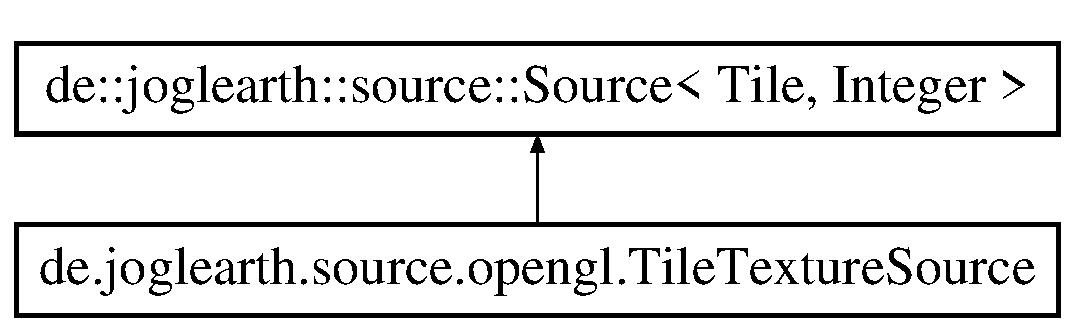
\includegraphics[height=2.000000cm]{classde_1_1joglearth_1_1source_1_1opengl_1_1_tile_texture_source}
\end{center}
\end{figure}
\subsection*{Öffentliche Methoden}
\begin{DoxyCompactItemize}
\item 
Source\-Response$<$ Integer $>$ {\bfseries request\-Object} ({\bf Tile} key, Source\-Listener$<$ {\bf Tile}, Integer $>$ sender)\label{classde_1_1joglearth_1_1source_1_1opengl_1_1_tile_texture_source_ad02bb08c1f25e54ddcd56e6ee48f799a}

\end{DoxyCompactItemize}


\subsection{Ausführliche Beschreibung}
Loads the textures into Open\-G\-L returning the I\-D. Implements \doxyref{Source}{S.}{} to get a new texture, when it is needed. Owns a \doxyref{Source}{S.}{} for image data. 
\section{de.\-joglearth.\-source.\-nominatim.\-Nominatim\-Query.\-Type Enum-\/\-Referenz}
\label{enumde_1_1joglearth_1_1source_1_1nominatim_1_1_nominatim_query_1_1_type}\index{de.\-joglearth.\-source.\-nominatim.\-Nominatim\-Query.\-Type@{de.\-joglearth.\-source.\-nominatim.\-Nominatim\-Query.\-Type}}
\subsection*{Öffentliche Attribute}
\begin{DoxyCompactItemize}
\item 
{\bf G\-L\-O\-B\-A\-L}
\item 
{\bf L\-O\-C\-A\-L}
\item 
{\bf P\-O\-I\-N\-T}
\end{DoxyCompactItemize}


\subsection{Ausführliche Beschreibung}
{\ttfamily \doxyref{Type}{S.}{enumde_1_1joglearth_1_1source_1_1nominatim_1_1_nominatim_query_1_1_type}} of the \doxyref{Nominatim\-Query}{S.}{classde_1_1joglearth_1_1source_1_1nominatim_1_1_nominatim_query}. 

\subsection{Dokumentation der Datenelemente}
\index{de\-::joglearth\-::source\-::nominatim\-::\-Nominatim\-Query\-::\-Type@{de\-::joglearth\-::source\-::nominatim\-::\-Nominatim\-Query\-::\-Type}!G\-L\-O\-B\-A\-L@{G\-L\-O\-B\-A\-L}}
\index{G\-L\-O\-B\-A\-L@{G\-L\-O\-B\-A\-L}!de::joglearth::source::nominatim::NominatimQuery::Type@{de\-::joglearth\-::source\-::nominatim\-::\-Nominatim\-Query\-::\-Type}}
\subsubsection[{G\-L\-O\-B\-A\-L}]{\setlength{\rightskip}{0pt plus 5cm}de.\-joglearth.\-source.\-nominatim.\-Nominatim\-Query.\-Type.\-G\-L\-O\-B\-A\-L}\label{enumde_1_1joglearth_1_1source_1_1nominatim_1_1_nominatim_query_1_1_type_a45fe33243ee568142437411e3edf88fa}
Global search of points. \index{de\-::joglearth\-::source\-::nominatim\-::\-Nominatim\-Query\-::\-Type@{de\-::joglearth\-::source\-::nominatim\-::\-Nominatim\-Query\-::\-Type}!L\-O\-C\-A\-L@{L\-O\-C\-A\-L}}
\index{L\-O\-C\-A\-L@{L\-O\-C\-A\-L}!de::joglearth::source::nominatim::NominatimQuery::Type@{de\-::joglearth\-::source\-::nominatim\-::\-Nominatim\-Query\-::\-Type}}
\subsubsection[{L\-O\-C\-A\-L}]{\setlength{\rightskip}{0pt plus 5cm}de.\-joglearth.\-source.\-nominatim.\-Nominatim\-Query.\-Type.\-L\-O\-C\-A\-L}\label{enumde_1_1joglearth_1_1source_1_1nominatim_1_1_nominatim_query_1_1_type_a95a118ae9bf01db12c1e8e5db8b60f12}
The results of the query are within the F\-O\-V. \index{de\-::joglearth\-::source\-::nominatim\-::\-Nominatim\-Query\-::\-Type@{de\-::joglearth\-::source\-::nominatim\-::\-Nominatim\-Query\-::\-Type}!P\-O\-I\-N\-T@{P\-O\-I\-N\-T}}
\index{P\-O\-I\-N\-T@{P\-O\-I\-N\-T}!de::joglearth::source::nominatim::NominatimQuery::Type@{de\-::joglearth\-::source\-::nominatim\-::\-Nominatim\-Query\-::\-Type}}
\subsubsection[{P\-O\-I\-N\-T}]{\setlength{\rightskip}{0pt plus 5cm}de.\-joglearth.\-source.\-nominatim.\-Nominatim\-Query.\-Type.\-P\-O\-I\-N\-T}\label{enumde_1_1joglearth_1_1source_1_1nominatim_1_1_nominatim_query_1_1_type_a0d0663f22170dad6f9dd39afd9f338da}
The result of the query is a point with x and y coordinates. 
\section{de.\-joglearth.\-source.\-caching.\-Unity\-Measure$<$ T $>$ Klassenreferenz}
\label{classde_1_1joglearth_1_1source_1_1caching_1_1_unity_measure_3_01_t_01_4}\index{de.\-joglearth.\-source.\-caching.\-Unity\-Measure$<$ T $>$@{de.\-joglearth.\-source.\-caching.\-Unity\-Measure$<$ T $>$}}
Klassendiagramm für de.\-joglearth.\-source.\-caching.\-Unity\-Measure$<$ T $>$\-:\begin{figure}[H]
\begin{center}
\leavevmode
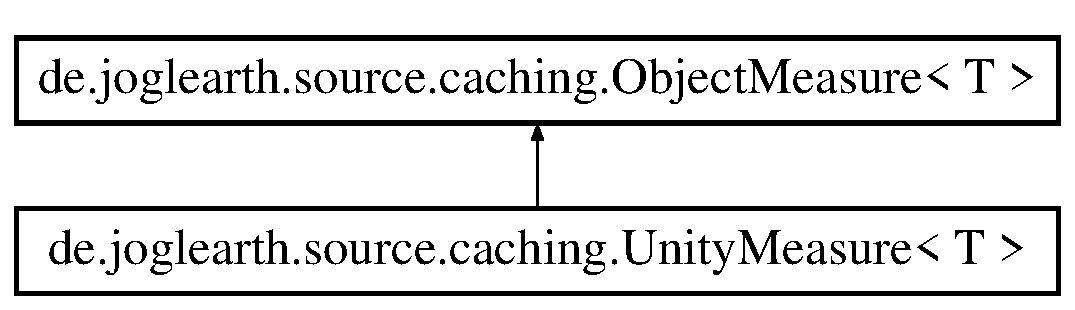
\includegraphics[height=2.000000cm]{classde_1_1joglearth_1_1source_1_1caching_1_1_unity_measure_3_01_t_01_4}
\end{center}
\end{figure}
\subsection*{Öffentliche Methoden}
\begin{DoxyCompactItemize}
\item 
int {\bf get\-Size} (T t)
\end{DoxyCompactItemize}


\subsection{Ausführliche Beschreibung}
Implements the \doxyref{de.\-joglearth.\-source.\-caching.\-Object\-Measure}{S.}{} interface in such way that it can measure the size of single objects. Treats every object as a object of the size 1.


\begin{DoxyParams}{Parameter}
{\em T} & The type of the measured object \\
\hline
\end{DoxyParams}


\subsection{Dokumentation der Elementfunktionen}
\index{de\-::joglearth\-::source\-::caching\-::\-Unity\-Measure$<$ T $>$@{de\-::joglearth\-::source\-::caching\-::\-Unity\-Measure$<$ T $>$}!get\-Size@{get\-Size}}
\index{get\-Size@{get\-Size}!de::joglearth::source::caching::UnityMeasure< T >@{de\-::joglearth\-::source\-::caching\-::\-Unity\-Measure$<$ T $>$}}
\subsubsection[{get\-Size}]{\setlength{\rightskip}{0pt plus 5cm}int de.\-joglearth.\-source.\-caching.\-Unity\-Measure$<$ T $>$.get\-Size (
\begin{DoxyParamCaption}
\item[{T}]{object}
\end{DoxyParamCaption}
)}\label{classde_1_1joglearth_1_1source_1_1caching_1_1_unity_measure_3_01_t_01_4_a2fe8769ef6b5b550d83169ef02eebb90}
Determines the size of an object in a unit specific to the implementing class.


\begin{DoxyParams}{Parameter}
{\em object} & The object to measure \\
\hline
\end{DoxyParams}
\begin{DoxyReturn}{Rückgabe}
The size, in units. Must be greater or equal 1 
\end{DoxyReturn}


Implementiert {\bf de.\-joglearth.\-source.\-caching.\-Object\-Measure$<$ T $>$} \doxyref{}{S.}{interfacede_1_1joglearth_1_1source_1_1caching_1_1_object_measure_3_01_t_01_4_a1d7e082d696fb43f94fbade17deb9f2c}.


\section{de.\-joglearth.\-geometry.\-Vector3 \-Klassenreferenz}
\label{classde_1_1joglearth_1_1geometry_1_1_vector3}\index{de.\-joglearth.\-geometry.\-Vector3@{de.\-joglearth.\-geometry.\-Vector3}}
\subsection*{Öffentliche \-Methoden}
\begin{DoxyCompactItemize}
\item 
{\bf \-Vector3} ()
\item 
{\bf \-Vector3} (double x, double y, double z)
\item 
{\bf \-Vector3} {\bf clone} ()
\item 
{\bf \-Vector3} {\bf to} ({\bf \-Vector3} other)
\item 
{\bf \-Vector3} {\bf times} (double c)
\item 
{\bf \-Vector3} {\bf plus} ({\bf \-Vector3} v)
\item 
{\bf \-Vector3} {\bf minus} ({\bf \-Vector3} v)
\item 
double {\bf length} ()
\item 
void {\bf add} ({\bf \-Vector3} v)
\item 
{\bf \-Vector3} {\bf normalized} ()
\item 
int {\bfseries hash\-Code} ()\label{classde_1_1joglearth_1_1geometry_1_1_vector3_a6443b06dbbda9a6996f21aab53571672}

\item 
boolean {\bfseries equals} (\-Object obj)\label{classde_1_1joglearth_1_1geometry_1_1_vector3_ab559c440e731cd083e1f8708fe0062ca}

\end{DoxyCompactItemize}
\subsection*{Öffentliche \-Attribute}
\begin{DoxyCompactItemize}
\item 
double {\bfseries x}\label{classde_1_1joglearth_1_1geometry_1_1_vector3_a3f2050e4ad0d81adb717429a87246377}

\item 
double {\bfseries y}\label{classde_1_1joglearth_1_1geometry_1_1_vector3_aa7f5535f1ac0cefcbaf1aa56d17f5f5e}

\item 
double {\bfseries z}\label{classde_1_1joglearth_1_1geometry_1_1_vector3_a18ed3b85836716833940d4fd412ff3e6}

\end{DoxyCompactItemize}


\subsection{\-Ausführliche \-Beschreibung}
\-A structure for 3-\/dimensional vectors in \-Cartesian coordinates. 

\subsection{\-Beschreibung der \-Konstruktoren und \-Destruktoren}
\index{de\-::joglearth\-::geometry\-::\-Vector3@{de\-::joglearth\-::geometry\-::\-Vector3}!\-Vector3@{\-Vector3}}
\index{\-Vector3@{\-Vector3}!de::joglearth::geometry::Vector3@{de\-::joglearth\-::geometry\-::\-Vector3}}
\subsubsection[{\-Vector3}]{\setlength{\rightskip}{0pt plus 5cm}{\bf de.\-joglearth.\-geometry.\-Vector3.\-Vector3} (
\begin{DoxyParamCaption}
{}
\end{DoxyParamCaption}
)}\label{classde_1_1joglearth_1_1geometry_1_1_vector3_a84ab3f388b5d1a290fa4db450265c862}
\-Constructor. \-Creates a zero vector. \index{de\-::joglearth\-::geometry\-::\-Vector3@{de\-::joglearth\-::geometry\-::\-Vector3}!\-Vector3@{\-Vector3}}
\index{\-Vector3@{\-Vector3}!de::joglearth::geometry::Vector3@{de\-::joglearth\-::geometry\-::\-Vector3}}
\subsubsection[{\-Vector3}]{\setlength{\rightskip}{0pt plus 5cm}{\bf de.\-joglearth.\-geometry.\-Vector3.\-Vector3} (
\begin{DoxyParamCaption}
\item[{double}]{x, }
\item[{double}]{y, }
\item[{double}]{z}
\end{DoxyParamCaption}
)}\label{classde_1_1joglearth_1_1geometry_1_1_vector3_afaa069b9ed2d163780939f6d93e1e1ad}
\-Constructor. \-Initializes a vector with the parameters provided.


\begin{DoxyParams}{\-Parameter}
{\em x} & \-The \-X (first) component. \\
\hline
{\em y} & \-The \-Y (second) component. \\
\hline
{\em z} & \-The \-Z (third) component. \\
\hline
\end{DoxyParams}


\subsection{\-Dokumentation der \-Elementfunktionen}
\index{de\-::joglearth\-::geometry\-::\-Vector3@{de\-::joglearth\-::geometry\-::\-Vector3}!add@{add}}
\index{add@{add}!de::joglearth::geometry::Vector3@{de\-::joglearth\-::geometry\-::\-Vector3}}
\subsubsection[{add}]{\setlength{\rightskip}{0pt plus 5cm}void {\bf de.\-joglearth.\-geometry.\-Vector3.\-add} (
\begin{DoxyParamCaption}
\item[{{\bf \-Vector3}}]{v}
\end{DoxyParamCaption}
)}\label{classde_1_1joglearth_1_1geometry_1_1_vector3_adea5176e0b73c83b74bbb139e40ac3c5}
\-Adds another vector to this vector. 
\begin{DoxyParams}{\-Parameter}
{\em v} & \-The vector to add. \\
\hline
\end{DoxyParams}
\index{de\-::joglearth\-::geometry\-::\-Vector3@{de\-::joglearth\-::geometry\-::\-Vector3}!clone@{clone}}
\index{clone@{clone}!de::joglearth::geometry::Vector3@{de\-::joglearth\-::geometry\-::\-Vector3}}
\subsubsection[{clone}]{\setlength{\rightskip}{0pt plus 5cm}{\bf \-Vector3} {\bf de.\-joglearth.\-geometry.\-Vector3.\-clone} (
\begin{DoxyParamCaption}
{}
\end{DoxyParamCaption}
)}\label{classde_1_1joglearth_1_1geometry_1_1_vector3_a6c9bdfdd9e73cb6cd56e784e12702341}
\-Creates a deep copy.

\begin{DoxyReturn}{\-Rückgabe}
\-An exact copy of the vector. 
\end{DoxyReturn}
\index{de\-::joglearth\-::geometry\-::\-Vector3@{de\-::joglearth\-::geometry\-::\-Vector3}!length@{length}}
\index{length@{length}!de::joglearth::geometry::Vector3@{de\-::joglearth\-::geometry\-::\-Vector3}}
\subsubsection[{length}]{\setlength{\rightskip}{0pt plus 5cm}double {\bf de.\-joglearth.\-geometry.\-Vector3.\-length} (
\begin{DoxyParamCaption}
{}
\end{DoxyParamCaption}
)}\label{classde_1_1joglearth_1_1geometry_1_1_vector3_a47bf183b1df757adffdd0991750390c4}
\-Calculates the vectors length, that is sqrt(x$^\wedge$2+y$^\wedge$2+z$^\wedge$2). \begin{DoxyReturn}{\-Rückgabe}
\-The length. 
\end{DoxyReturn}
\index{de\-::joglearth\-::geometry\-::\-Vector3@{de\-::joglearth\-::geometry\-::\-Vector3}!minus@{minus}}
\index{minus@{minus}!de::joglearth::geometry::Vector3@{de\-::joglearth\-::geometry\-::\-Vector3}}
\subsubsection[{minus}]{\setlength{\rightskip}{0pt plus 5cm}{\bf \-Vector3} {\bf de.\-joglearth.\-geometry.\-Vector3.\-minus} (
\begin{DoxyParamCaption}
\item[{{\bf \-Vector3}}]{v}
\end{DoxyParamCaption}
)}\label{classde_1_1joglearth_1_1geometry_1_1_vector3_ae5d57a22ab35a8b2e23723261c3f6399}
\-Calculates the difference vector to another \-Vecotr3. 
\begin{DoxyParams}{\-Parameter}
{\em v} & \-The vector to subtract. \\
\hline
\end{DoxyParams}
\begin{DoxyReturn}{\-Rückgabe}
\-The difference. 
\end{DoxyReturn}
\index{de\-::joglearth\-::geometry\-::\-Vector3@{de\-::joglearth\-::geometry\-::\-Vector3}!normalized@{normalized}}
\index{normalized@{normalized}!de::joglearth::geometry::Vector3@{de\-::joglearth\-::geometry\-::\-Vector3}}
\subsubsection[{normalized}]{\setlength{\rightskip}{0pt plus 5cm}{\bf \-Vector3} {\bf de.\-joglearth.\-geometry.\-Vector3.\-normalized} (
\begin{DoxyParamCaption}
{}
\end{DoxyParamCaption}
)}\label{classde_1_1joglearth_1_1geometry_1_1_vector3_abafe54075c2af1b22d7485733fb12283}
\-Normalizes the vector, so that \doxyref{length()}{\-S.}{classde_1_1joglearth_1_1geometry_1_1_vector3_a47bf183b1df757adffdd0991750390c4} == 1. \begin{DoxyReturn}{\-Rückgabe}

\end{DoxyReturn}
\index{de\-::joglearth\-::geometry\-::\-Vector3@{de\-::joglearth\-::geometry\-::\-Vector3}!plus@{plus}}
\index{plus@{plus}!de::joglearth::geometry::Vector3@{de\-::joglearth\-::geometry\-::\-Vector3}}
\subsubsection[{plus}]{\setlength{\rightskip}{0pt plus 5cm}{\bf \-Vector3} {\bf de.\-joglearth.\-geometry.\-Vector3.\-plus} (
\begin{DoxyParamCaption}
\item[{{\bf \-Vector3}}]{v}
\end{DoxyParamCaption}
)}\label{classde_1_1joglearth_1_1geometry_1_1_vector3_a22fca4a8ad0e84578402d239b43a154e}
\-Calculates the sum of this and a second vector. 
\begin{DoxyParams}{\-Parameter}
{\em v} & \-The vector to add. \\
\hline
\end{DoxyParams}
\begin{DoxyReturn}{\-Rückgabe}
\-The sum. 
\end{DoxyReturn}
\index{de\-::joglearth\-::geometry\-::\-Vector3@{de\-::joglearth\-::geometry\-::\-Vector3}!times@{times}}
\index{times@{times}!de::joglearth::geometry::Vector3@{de\-::joglearth\-::geometry\-::\-Vector3}}
\subsubsection[{times}]{\setlength{\rightskip}{0pt plus 5cm}{\bf \-Vector3} {\bf de.\-joglearth.\-geometry.\-Vector3.\-times} (
\begin{DoxyParamCaption}
\item[{double}]{c}
\end{DoxyParamCaption}
)}\label{classde_1_1joglearth_1_1geometry_1_1_vector3_a4a3580e21ee8ebdc80a7a56cdf45b303}
\-Multiplies the vector by a scalar. 
\begin{DoxyParams}{\-Parameter}
{\em c} & \-The scalar. \\
\hline
\end{DoxyParams}
\begin{DoxyReturn}{\-Rückgabe}
\-The product vector. 
\end{DoxyReturn}
\index{de\-::joglearth\-::geometry\-::\-Vector3@{de\-::joglearth\-::geometry\-::\-Vector3}!to@{to}}
\index{to@{to}!de::joglearth::geometry::Vector3@{de\-::joglearth\-::geometry\-::\-Vector3}}
\subsubsection[{to}]{\setlength{\rightskip}{0pt plus 5cm}{\bf \-Vector3} {\bf de.\-joglearth.\-geometry.\-Vector3.\-to} (
\begin{DoxyParamCaption}
\item[{{\bf \-Vector3}}]{other}
\end{DoxyParamCaption}
)}\label{classde_1_1joglearth_1_1geometry_1_1_vector3_a6e61b26f95647b79ca50d58c41c25435}
\-Calculates the difference vector from another \doxyref{\-Vector3}{\-S.}{classde_1_1joglearth_1_1geometry_1_1_vector3}. 
\begin{DoxyParams}{\-Parameter}
{\em other} & \-The vector to subtract from. \\
\hline
\end{DoxyParams}
\begin{DoxyReturn}{\-Rückgabe}
\-The difference. 
\end{DoxyReturn}

\section{de.\-joglearth.\-geometry.\-Vector4 \-Klassenreferenz}
\label{classde_1_1joglearth_1_1geometry_1_1_vector4}\index{de.\-joglearth.\-geometry.\-Vector4@{de.\-joglearth.\-geometry.\-Vector4}}
\subsection*{Öffentliche \-Methoden}
\begin{DoxyCompactItemize}
\item 
{\bf \-Vector4} ()
\item 
{\bf \-Vector4} (double {\bf x}, double {\bf y}, double {\bf z}, double {\bf w})
\item 
{\bf \-Vector4} ({\bf \-Vector3} copy\-From)
\item 
{\bf \-Vector3} {\bf divide} ()
\item 
\-String {\bfseries to\-String} ()\label{classde_1_1joglearth_1_1geometry_1_1_vector4_ac09e3af7012cbcefff485d6c0c78667a}

\item 
int {\bfseries hash\-Code} ()\label{classde_1_1joglearth_1_1geometry_1_1_vector4_a171d3d8eeb912579e61a750b72b41820}

\item 
boolean {\bfseries equals} (\-Object obj)\label{classde_1_1joglearth_1_1geometry_1_1_vector4_a25acec04eb4a9544e8873c1df2ae31c2}

\end{DoxyCompactItemize}
\subsection*{Öffentliche \-Attribute}
\begin{DoxyCompactItemize}
\item 
double {\bf x}
\item 
double {\bf y}
\item 
double {\bf z}
\item 
double {\bf w}
\end{DoxyCompactItemize}


\subsection{\-Ausführliche \-Beschreibung}
\-A structure for 4-\/dimensional vectors in homogeneous coordinates. 

\subsection{\-Beschreibung der \-Konstruktoren und \-Destruktoren}
\index{de\-::joglearth\-::geometry\-::\-Vector4@{de\-::joglearth\-::geometry\-::\-Vector4}!\-Vector4@{\-Vector4}}
\index{\-Vector4@{\-Vector4}!de::joglearth::geometry::Vector4@{de\-::joglearth\-::geometry\-::\-Vector4}}
\subsubsection[{\-Vector4}]{\setlength{\rightskip}{0pt plus 5cm}{\bf de.\-joglearth.\-geometry.\-Vector4.\-Vector4} (
\begin{DoxyParamCaption}
{}
\end{DoxyParamCaption}
)}\label{classde_1_1joglearth_1_1geometry_1_1_vector4_aef0f28577f39c7eb02ad45b8decc14e6}
\-Default constructor. \-Initializes a zero vector with scaling factor 1.

\-The resulting vector will have x=0, y=0, z=0, w=1. \index{de\-::joglearth\-::geometry\-::\-Vector4@{de\-::joglearth\-::geometry\-::\-Vector4}!\-Vector4@{\-Vector4}}
\index{\-Vector4@{\-Vector4}!de::joglearth::geometry::Vector4@{de\-::joglearth\-::geometry\-::\-Vector4}}
\subsubsection[{\-Vector4}]{\setlength{\rightskip}{0pt plus 5cm}{\bf de.\-joglearth.\-geometry.\-Vector4.\-Vector4} (
\begin{DoxyParamCaption}
\item[{double}]{x, }
\item[{double}]{y, }
\item[{double}]{z, }
\item[{double}]{w}
\end{DoxyParamCaption}
)}\label{classde_1_1joglearth_1_1geometry_1_1_vector4_af2bec15f21d9355104714d591efca7b7}
\-Constructor.


\begin{DoxyParams}{\-Parameter}
{\em x} & \-The first component (this.\-x). \\
\hline
{\em y} & \-The second component (this.\-y). \\
\hline
{\em z} & \-The third component (this.\-z). \\
\hline
{\em w} & \-The scaling factor (this.\-w). \\
\hline
\end{DoxyParams}
\index{de\-::joglearth\-::geometry\-::\-Vector4@{de\-::joglearth\-::geometry\-::\-Vector4}!\-Vector4@{\-Vector4}}
\index{\-Vector4@{\-Vector4}!de::joglearth::geometry::Vector4@{de\-::joglearth\-::geometry\-::\-Vector4}}
\subsubsection[{\-Vector4}]{\setlength{\rightskip}{0pt plus 5cm}{\bf de.\-joglearth.\-geometry.\-Vector4.\-Vector4} (
\begin{DoxyParamCaption}
\item[{{\bf \-Vector3}}]{copy\-From}
\end{DoxyParamCaption}
)}\label{classde_1_1joglearth_1_1geometry_1_1_vector4_ab21bf2e030b969308b87162b84111f3e}
\-Constructor copying the position from a \doxyref{\-Vector3}{\-S.}{classde_1_1joglearth_1_1geometry_1_1_vector3}. \-The scaling factor w is set to 1.


\begin{DoxyParams}{\-Parameter}
{\em copy\-From} & \-The vector to copy from. \\
\hline
\end{DoxyParams}


\subsection{\-Dokumentation der \-Elementfunktionen}
\index{de\-::joglearth\-::geometry\-::\-Vector4@{de\-::joglearth\-::geometry\-::\-Vector4}!divide@{divide}}
\index{divide@{divide}!de::joglearth::geometry::Vector4@{de\-::joglearth\-::geometry\-::\-Vector4}}
\subsubsection[{divide}]{\setlength{\rightskip}{0pt plus 5cm}{\bf \-Vector3} {\bf de.\-joglearth.\-geometry.\-Vector4.\-divide} (
\begin{DoxyParamCaption}
{}
\end{DoxyParamCaption}
)}\label{classde_1_1joglearth_1_1geometry_1_1_vector4_a9c46bb2498e82e0b2a28a8bad0406bb1}
\-Creates a three-\/dimensional vector by dividing (x,y,z) by the scaling factor w.

\begin{DoxyReturn}{\-Rückgabe}
\-The scaled three-\/dimensional vector. 
\end{DoxyReturn}


\subsection{\-Dokumentation der \-Datenelemente}
\index{de\-::joglearth\-::geometry\-::\-Vector4@{de\-::joglearth\-::geometry\-::\-Vector4}!w@{w}}
\index{w@{w}!de::joglearth::geometry::Vector4@{de\-::joglearth\-::geometry\-::\-Vector4}}
\subsubsection[{w}]{\setlength{\rightskip}{0pt plus 5cm}double {\bf de.\-joglearth.\-geometry.\-Vector4.\-w}}\label{classde_1_1joglearth_1_1geometry_1_1_vector4_acf93eceaadf2301848b91352caedea3c}
\-The scaling factor. \index{de\-::joglearth\-::geometry\-::\-Vector4@{de\-::joglearth\-::geometry\-::\-Vector4}!x@{x}}
\index{x@{x}!de::joglearth::geometry::Vector4@{de\-::joglearth\-::geometry\-::\-Vector4}}
\subsubsection[{x}]{\setlength{\rightskip}{0pt plus 5cm}double {\bf de.\-joglearth.\-geometry.\-Vector4.\-x}}\label{classde_1_1joglearth_1_1geometry_1_1_vector4_a100feeea55a945d8d59aba95d1b113fc}
\-The first (\-X) component. \index{de\-::joglearth\-::geometry\-::\-Vector4@{de\-::joglearth\-::geometry\-::\-Vector4}!y@{y}}
\index{y@{y}!de::joglearth::geometry::Vector4@{de\-::joglearth\-::geometry\-::\-Vector4}}
\subsubsection[{y}]{\setlength{\rightskip}{0pt plus 5cm}double {\bf de.\-joglearth.\-geometry.\-Vector4.\-y}}\label{classde_1_1joglearth_1_1geometry_1_1_vector4_a30f3cc3accf392826e1beee439583802}
\-The second (\-Y) component. \index{de\-::joglearth\-::geometry\-::\-Vector4@{de\-::joglearth\-::geometry\-::\-Vector4}!z@{z}}
\index{z@{z}!de::joglearth::geometry::Vector4@{de\-::joglearth\-::geometry\-::\-Vector4}}
\subsubsection[{z}]{\setlength{\rightskip}{0pt plus 5cm}double {\bf de.\-joglearth.\-geometry.\-Vector4.\-z}}\label{classde_1_1joglearth_1_1geometry_1_1_vector4_afb069fbe322710e8f4a699ba239c91b0}
\-The third (\-Z) component. 
\section{de.\-joglearth.\-source.\-opengl.\-Vertex\-Buffer\-Cache Klassenreferenz}
\label{classde_1_1joglearth_1_1source_1_1opengl_1_1_vertex_buffer_cache}\index{de.\-joglearth.\-source.\-opengl.\-Vertex\-Buffer\-Cache@{de.\-joglearth.\-source.\-opengl.\-Vertex\-Buffer\-Cache}}
Klassendiagramm für de.\-joglearth.\-source.\-opengl.\-Vertex\-Buffer\-Cache\-:\begin{figure}[H]
\begin{center}
\leavevmode
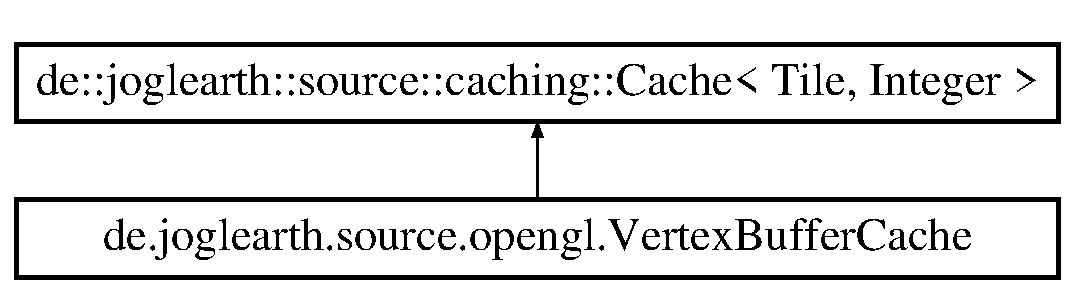
\includegraphics[height=2.000000cm]{classde_1_1joglearth_1_1source_1_1opengl_1_1_vertex_buffer_cache}
\end{center}
\end{figure}
\subsection*{Öffentliche Methoden}
\begin{DoxyCompactItemize}
\item 
{\bf Vertex\-Buffer\-Cache} (G\-L2 gl)
\item 
Source\-Response$<$ Integer $>$ {\bfseries request\-Object} ({\bf Tile} key, Source\-Listener$<$ {\bf Tile}, Integer $>$ sender)\label{classde_1_1joglearth_1_1source_1_1opengl_1_1_vertex_buffer_cache_af5bd1090210a2a3965b5f923d4d25cf3}

\item 
void {\bfseries put\-Object} ({\bf Tile} k, Integer v)\label{classde_1_1joglearth_1_1source_1_1opengl_1_1_vertex_buffer_cache_a8d15fb002c3670d792d3d4afc2a99e77}

\item 
void {\bfseries drop\-Object} ({\bf Tile} k)\label{classde_1_1joglearth_1_1source_1_1opengl_1_1_vertex_buffer_cache_acb75192f943155b456587cf0263811f5}

\item 
Iterable$<$ {\bf Tile} $>$ {\bfseries get\-Existing\-Objects} ()\label{classde_1_1joglearth_1_1source_1_1opengl_1_1_vertex_buffer_cache_a5b176c65220e0121d8c2fa6ed094004a}

\item 
void {\bfseries drop\-All} ()\label{classde_1_1joglearth_1_1source_1_1opengl_1_1_vertex_buffer_cache_a76d2df5358cefaae96416a0016d71585}

\end{DoxyCompactItemize}


\subsection{Ausführliche Beschreibung}
Manages and displaces vertex buffer objects in Open\-Gl graphics memory. 

\subsection{Beschreibung der Konstruktoren und Destruktoren}
\index{de\-::joglearth\-::source\-::opengl\-::\-Vertex\-Buffer\-Cache@{de\-::joglearth\-::source\-::opengl\-::\-Vertex\-Buffer\-Cache}!Vertex\-Buffer\-Cache@{Vertex\-Buffer\-Cache}}
\index{Vertex\-Buffer\-Cache@{Vertex\-Buffer\-Cache}!de::joglearth::source::opengl::VertexBufferCache@{de\-::joglearth\-::source\-::opengl\-::\-Vertex\-Buffer\-Cache}}
\subsubsection[{Vertex\-Buffer\-Cache}]{\setlength{\rightskip}{0pt plus 5cm}de.\-joglearth.\-source.\-opengl.\-Vertex\-Buffer\-Cache.\-Vertex\-Buffer\-Cache (
\begin{DoxyParamCaption}
\item[{G\-L2}]{gl}
\end{DoxyParamCaption}
)}\label{classde_1_1joglearth_1_1source_1_1opengl_1_1_vertex_buffer_cache_a390dcaaf59a575d03e1d6606d7c4bebf}
Constructor. Initializes the \doxyref{Vertex\-Buffer\-Cache}{S.}{classde_1_1joglearth_1_1source_1_1opengl_1_1_vertex_buffer_cache} and assigns a value to the G\-L context.


\begin{DoxyParams}{Parameter}
{\em gl} & The G\-L context \\
\hline
\end{DoxyParams}

\section{de.\-joglearth.\-ui.\-View\-Event\-Listener Klassenreferenz}
\label{classde_1_1joglearth_1_1ui_1_1_view_event_listener}\index{de.\-joglearth.\-ui.\-View\-Event\-Listener@{de.\-joglearth.\-ui.\-View\-Event\-Listener}}


Abgeleitet von Mouse\-Wheel\-Listener, Mouse\-Listener und Mouse\-Motion\-Listener.

\subsection*{Öffentliche Methoden}
\begin{DoxyCompactItemize}
\item 
{\bf View\-Event\-Listener} ({\bf Camera} camera)
\item 
void {\bfseries mouse\-Dragged} (Mouse\-Event e)\label{classde_1_1joglearth_1_1ui_1_1_view_event_listener_adb92b3ef84b19c09cc3f949b3cb574cc}

\item 
void {\bfseries mouse\-Moved} (Mouse\-Event e)\label{classde_1_1joglearth_1_1ui_1_1_view_event_listener_a9a88da68f17ebe909defd9c678be83e9}

\item 
void {\bfseries mouse\-Clicked} (Mouse\-Event e)\label{classde_1_1joglearth_1_1ui_1_1_view_event_listener_a137174da74d9f8bab35bfce09670023a}

\item 
void {\bfseries mouse\-Entered} (Mouse\-Event e)\label{classde_1_1joglearth_1_1ui_1_1_view_event_listener_a01cfa6b91bd9fd8f3f42a67a0ca9ad1b}

\item 
void {\bfseries mouse\-Exited} (Mouse\-Event e)\label{classde_1_1joglearth_1_1ui_1_1_view_event_listener_aea0f67417443084c8efe7f8fb0f35a1f}

\item 
void {\bfseries mouse\-Pressed} (Mouse\-Event e)\label{classde_1_1joglearth_1_1ui_1_1_view_event_listener_a5d7004d272cf5557aa33ca6d466cb0f2}

\item 
void {\bfseries mouse\-Released} (Mouse\-Event e)\label{classde_1_1joglearth_1_1ui_1_1_view_event_listener_a949577b85d1209c9509f57f8ae4ffa6d}

\item 
void {\bfseries mouse\-Wheel\-Moved} (Mouse\-Wheel\-Event e)\label{classde_1_1joglearth_1_1ui_1_1_view_event_listener_aa52167a5317d07456699ab30d77cf739}

\end{DoxyCompactItemize}


\subsection{Ausführliche Beschreibung}
An Object of this class is used to handle user interaction that occurs on the \doxyref{G\-L\-Canvas}{S.}{}. 

\subsection{Beschreibung der Konstruktoren und Destruktoren}
\index{de\-::joglearth\-::ui\-::\-View\-Event\-Listener@{de\-::joglearth\-::ui\-::\-View\-Event\-Listener}!View\-Event\-Listener@{View\-Event\-Listener}}
\index{View\-Event\-Listener@{View\-Event\-Listener}!de::joglearth::ui::ViewEventListener@{de\-::joglearth\-::ui\-::\-View\-Event\-Listener}}
\subsubsection[{View\-Event\-Listener}]{\setlength{\rightskip}{0pt plus 5cm}de.\-joglearth.\-ui.\-View\-Event\-Listener.\-View\-Event\-Listener (
\begin{DoxyParamCaption}
\item[{{\bf Camera}}]{camera}
\end{DoxyParamCaption}
)}\label{classde_1_1joglearth_1_1ui_1_1_view_event_listener_af6ff662f148b0139015c12ad4885a907}
Constructor taking a \doxyref{Camera}{S.}{} object that the movements will be applied on.


\begin{DoxyParams}{Parameter}
{\em camera} & the {\ttfamily Camera} \\
\hline
\end{DoxyParams}

%--- End generated contents ---

\chapter{JUnit Tests}

\chapter{Algorithmen}

\chapter{Persistente Daten}

\section{Liste der POIs}

\vspace{1.5 cm}
\begin{tabular}{|c|c|c|}
\hline 
\rule[-1ex]{0pt}{4ex} \textbf{ENUM} & \textbf{Erklärung} & \textbf{Overpass Query} \\ 
\hline  \hline
\rule[-1ex]{0pt}{4ex} RESTAURANT & Liefert Cafes, Restaurants und Biergärten &  \\ 
\hline
\rule[-1ex]{0pt}{4ex} NIGHTLIFE & Liefert Bars, Clubs, Diskotheken, Kinos, Casinos und Solarien &  \\ 
\hline
\rule[-1ex]{0pt}{4ex}  BANK & Liefert Banken und Sparkassen &  \\ 
\hline
\rule[-1ex]{0pt}{4ex} FOOD & Liefert Supermärkte, Bäcker, Metzger und Drogerien &  \\ 
\hline
\rule[-1ex]{0pt}{4ex} SHOPS & Liefert Geschäfte aller Art. &  \\ 
\hline
\rule[-1ex]{0pt}{4ex} ACTIVITY & Liefert Freizeitaktivitäten, Picknickplätze und Aussichtspunkte &  \\ 
\hline
\rule[-1ex]{0pt}{4ex} EDUCATION & Liefert Bildungseinrichtungen &  \\ 
\hline
\rule[-1ex]{0pt}{4ex} HEALTH & Liefert Ärzte, Krankenhäuser, Apotheken und Drogerien &  \\ 
\hline
\rule[-1ex]{0pt}{4ex} UTILS &  &  \\ 
\hline
\rule[-1ex]{0pt}{4ex} HOTELS &  &  \\ 
\hline
\end{tabular}


\chapter{Übersetzung der Bedienoberfläche}
\begin{tabular}{|p{7.5cm}|p{7.5cm}|}
\hline 
\textbf{Deutsch} & \textbf{Englisch} \\ 
\hline
\hline 
Ansicht & view \\ 
\hline
Ansichtsmodus & mode \\ 
\hline
Sonnensystem & solarsystem \\
\hline
Satellitenbild & satellite mode \\
\hline
Höhenprofil & heightmap \\
\hline
Für diesen Ort sind keine Informationen verfügbar & No information available to this point. \\
\hline
Punkt markieren & mark point\\
\hline
Längengrad & Longitude \\
\hline
Breitengrad & Latitude \\
\hline
km (Kilometer) & km \\
\hline
Globus & globe \\
\hline
Karte & map \\
\hline
Kinderweltkarte & world map for kids \\
\hline
Ort & place \\
\hline
Suche & search \\
\hline
Ort eingeben & insert place \\
\hline
in der Umgebung & surrounding \\
\hline
Global & global \\
\hline
Suchergebnisse & search results \\
\hline
Markierte Punkte & marked point \\
\hline
Angezeigte Beschriftungen & displaying labels \\
\hline
Markierung entfernen & remove marker \\
\hline
Einstellungen & settings \\
\hline
Sprache & language \\
\hline
Deutsch & german \\
\hline
Englisch & english \\
\hline
Grafikeinstellungen & graphic settings \\
\hline
Antialiasing & Antialiasing \\
\hline
Texturfilter & texture filter \\
\hline
Detaillevel & level of detail \\
\hline
an - aus & on - off \\
\hline
niedrig - mittel - hoch & low - medium - high\\
\hline
Cachegröße & cache size \\
\hline
Arbeitsspeicher & memory \\
\hline
Dateisystem & filesystem \\
\hline
Handbuch & manual \\
\hline
Info & info \\
\hline
Name & name \\
\hline
Name eingeben & insert name \\
\hline
Beschreibung & description \\
\hline
\end{tabular} 
\end{document}